%********************************************%
%*       Generated from PreTeXt source      *%
%*       on 2025-04-03T21:06:53-06:00       *%
%*   A recent stable commit (2022-07-01):   *%
%* 6c761d3dba23af92cba35001c852aac04ae99a5f *%
%*                                          *%
%*         https://pretextbook.org          *%
%*                                          *%
%********************************************%
% This document was created with the texstyle file "ams.xml" to satisfy the requirements of the journal "AMS journals."
%
%
\documentclass{amsart}
%
%% add a \support command as unnumbered footnote
\let\svdthefootnote\thefootnote%
\newcommand\support[1]{%
  \let\thefootnote\relax%
  \footnotetext{#1}%
  \let\thefootnote\svdthefootnote%
}
%% Custom Preamble Entries, early (use latex.preamble.early)
%% Always open on odd page
%%   The following adjusts cleardoublepage to remove twosided
%%   check so that we open on odd pages even in one-sided mode
%%   by adding an extra blank page on the preceding even page.
\makeatletter%
\def\cleardoublepage{%
\clearpage\ifodd\c@page\else\thispagestyle{empty}\hbox{}\newpage\if@twocolumn\hbox{}\newpage\fi\fi%
}
\makeatother%
%% Default LaTeX packages
%%   1.  always employed (or nearly so) for some purpose, or
%%   2.  a stylewriter may assume their presence
\usepackage{geometry}
%% Some aspects of the preamble are conditional,
%% the LaTeX engine is one such determinant
\usepackage{ifthen}
%% etoolbox has a variety of modern conveniences
\usepackage{etoolbox}
\usepackage{ifxetex,ifluatex}
%% Raster graphics inclusion
\usepackage{graphicx}
%% Color support, xcolor package
%% Always loaded, for: add/delete text, author tools
%% Here, since tcolorbox loads tikz, and tikz loads xcolor
\PassOptionsToPackage{dvipsnames,svgnames,table}{xcolor}
\usepackage{xcolor}
%% begin: defined colors, via xcolor package, for styling
%% end: defined colors, via xcolor package, for styling
%
\theoremstyle{plain}%
\newtheorem{theorem}{Theorem}[section]
\newtheorem{proposition}[theorem]{Conundrum}
\newtheorem{lemma}[theorem]{Lemma}
\newtheorem{corollary}[theorem]{Corollary}
\newtheorem{claim}[theorem]{Claim}
\newtheorem{fact}[theorem]{Fact}
\newtheorem{identity}[theorem]{Identity}
\newtheorem{conjecture}[theorem]{Conjecture}
%
\theoremstyle{definition}%
\newtheorem{definition}[theorem]{Definition}
\newtheorem{axiom}[theorem]{Axiom}
\newtheorem{principle}[theorem]{Principle}
\newtheorem{heuristic}[theorem]{Heuristic}
\newtheorem{hypothesis}[theorem]{Hypothesis}
\newtheorem{assumption}[theorem]{Assumption}
\newtheorem{openproblem}[theorem]{Open Problem}
\newtheorem{algorithm}[theorem]{Algorithm}
\newtheorem{question}[theorem]{Question}
\newtheorem{activity}[theorem]{Activity}
\newtheorem{inlineexercise}[theorem]{Checkpoint}
\newtheorem{investigation}[theorem]{Investigation}
\newtheorem{exploration}[theorem]{Exploration}
\newtheorem{problem}[theorem]{Problem}
\newtheorem{example}[theorem]{Example}
\newtheorem{project}[theorem]{Project}
%
\theoremstyle{remark}%
\newtheorem{remark}[theorem]{Remark}
\newtheorem{warning}[theorem]{Warning}
\newtheorem{convention}[theorem]{Convention}
\newtheorem{insight}[theorem]{Insight}
\newtheorem{note}[theorem]{Note}
\newtheorem{observation}[theorem]{Observation}
\newtheorem{computation}[theorem]{Computation}
\newtheorem{technology}[theorem]{Technology}
\newtheorem{data}[theorem]{Data}
%% Colored boxes, and much more, though mostly styling
%% skins library provides "enhanced" skin, employing tikzpicture
%% boxes may be configured as "breakable" or "unbreakable"
%% "raster" controls grids of boxes, aka side-by-side
\usepackage{tcolorbox}
\tcbuselibrary{skins}
\tcbuselibrary{breakable}
\tcbuselibrary{raster}
%% We load some "stock" tcolorbox styles that we use a lot
%% Placement here is provisional, there will be some color work also
%% First, black on white, no border, transparent, but no assumption about titles
\tcbset{ bwminimalstyle/.style={size=minimal, boxrule=-0.3pt, frame empty,
colback=white, colbacktitle=white, coltitle=black, opacityfill=0.0} }
%% Second, bold title, run-in to text/paragraph/heading
%% Space afterwards will be controlled by environment,
%% independent of constructions of the tcb title
%% Places \blocktitlefont onto many block titles
\tcbset{ runintitlestyle/.style={fonttitle=\blocktitlefont\upshape\bfseries, attach title to upper} }
%% Spacing prior to each exercise, anywhere
\tcbset{ exercisespacingstyle/.style={before skip={1.5ex plus 0.5ex}} }
%% Spacing prior to each block
\tcbset{ blockspacingstyle/.style={before skip={2.0ex plus 0.5ex}} }
%% xparse allows the construction of more robust commands,
%% this is a necessity for isolating styling and behavior
%% The tcolorbox library of the same name loads the base library
\tcbuselibrary{xparse}
%% The tcolorbox library loads TikZ, its calc package is generally useful,
%% and is necessary for some smaller documents that use partial tcolor boxes
%% See:  https://github.com/PreTeXtBook/pretext/issues/1624
\usetikzlibrary{calc}
%% We use some more exotic tcolorbox keys to restore indentation to parboxes
\tcbuselibrary{hooks}
%% assemblage: fairly simple un-numbered block/structure
\tcbset{ assemblagestyle/.style={size=normal, colback=white, colbacktitle=white, coltitle=black, colframe=black, rounded corners, titlerule=0.0pt, center title, fonttitle=\blocktitlefont\bfseries, blockspacingstyle, } }
\newtcolorbox{assemblage}[1][]{title={#1}, breakable, before upper app={\setparstyle}, assemblagestyle}
%%
%% tcolorbox, with styles, for ASIDE-LIKE
%%
%% aside: fairly simple un-numbered block/structure
\tcbset{ asidestyle/.style={bwminimalstyle, runintitlestyle, blockspacingstyle, after title={\space}, before upper app={\setparstyle}, } }
\newtcolorbox{aside}[1][]{title={#1}, breakable, before upper app={\setparstyle}, asidestyle}
%% biographical: fairly simple un-numbered block/structure
\tcbset{ biographicalstyle/.style={bwminimalstyle, runintitlestyle, blockspacingstyle, after title={\space}, before upper app={\setparstyle}, } }
\newtcolorbox{biographical}[1][]{title={#1}, breakable, before upper app={\setparstyle}, biographicalstyle}
%% historical: fairly simple un-numbered block/structure
\tcbset{ historicalstyle/.style={bwminimalstyle, runintitlestyle, blockspacingstyle, after title={\space}, before upper app={\setparstyle}, } }
\newtcolorbox{historical}[1][]{title={#1}, breakable, before upper app={\setparstyle}, historicalstyle}
%% Save default paragraph indentation and parskip for use later, when adjusting parboxes
\newlength{\ptxnormalparindent}
\newlength{\ptxnormalparskip}
\AtBeginDocument{\setlength{\ptxnormalparindent}{\parindent}}
\AtBeginDocument{\setlength{\ptxnormalparskip}{\parskip}}
\newcommand{\setparstyle}{\setlength{\parindent}{\ptxnormalparindent}\setlength{\parskip}{\ptxnormalparskip}}%% shorter subnumbers in some side-by-side require manipulations
\usepackage{xstring}
%% Custom Page Layout Adjustments (use publisher page-geometry entry)
%% This LaTeX file may be compiled with pdflatex, xelatex, or lualatex executables
%% LuaTeX is not explicitly supported, but we do accept additions from knowledgeable users
%% The conditional below provides  pdflatex  specific configuration last
%% begin: engine-specific capabilities
\ifthenelse{\boolean{xetex} \or \boolean{luatex}}{%
%% begin: xelatex and lualatex-specific default configuration
\ifxetex\usepackage{xltxtra}\fi
%% realscripts is the only part of xltxtra relevant to lualatex 
\ifluatex\usepackage{realscripts}\fi
%% end:   xelatex and lualatex-specific default configuration
}{
%% begin: pdflatex-specific default configuration
%% We assume a PreTeXt XML source file may have Unicode characters
%% and so we ask LaTeX to parse a UTF-8 encoded file
%% This may work well for accented characters in Western language,
%% but not with Greek, Asian languages, etc.
%% When this is not good enough, switch to the  xelatex  engine
%% where Unicode is better supported (encouraged, even)
\usepackage[utf8]{inputenc}
%% end: pdflatex-specific default configuration
}
%% end:   engine-specific capabilities
%%
%% Fonts.  Conditional on LaTex engine employed.
%% Default Text Font: The Latin Modern fonts are
%% "enhanced versions of the [original TeX] Computer Modern fonts."
%% We use them as the default text font for PreTeXt output.
%% Default Monospace font: Inconsolata (aka zi4)
%% Sponsored by TUG: http://levien.com/type/myfonts/inconsolata.html
%% Loaded for documents with intentional objects requiring monospace
%% See package documentation for excellent instructions
%% fontspec will work universally if we use filename to locate OTF files
%% Loads the "upquote" package as needed, so we don't have to
%% Upright quotes might come from the  textcomp  package, which we also use
%% We employ the shapely \ell to match Google Font version
%% pdflatex: "varl" package option produces shapely \ell
%% pdflatex: "var0" package option produces plain zero (not used)
%% pdflatex: "varqu" package option produces best upright quotes
%% xelatex,lualatex: add OTF StylisticSet 1 for shapely \ell
%% xelatex,lualatex: add OTF StylisticSet 2 for plain zero (not used)
%% xelatex,lualatex: add OTF StylisticSet 3 for upright quotes
%%
%% Automatic Font Control
%% Portions of a document, are, or may, be affected by defined commands
%% These are perhaps more flexible when using  xelatex  rather than  pdflatex
%% The following definitions are meant to be re-defined in a style, using \renewcommand
%% They are scoped when employed (in a TeX group), and so should not be defined with an argument
\newcommand{\divisionfont}{\relax}
\newcommand{\blocktitlefont}{\relax}
\newcommand{\contentsfont}{\relax}
\newcommand{\pagefont}{\relax}
\newcommand{\tabularfont}{\relax}
\newcommand{\xreffont}{\relax}
\newcommand{\titlepagefont}{\relax}
%%
\ifthenelse{\boolean{xetex} \or \boolean{luatex}}{%
%% begin: font setup and configuration for use with xelatex
%% Generally, xelatex is necessary for non-Western fonts
%% fontspec package provides extensive control of system fonts,
%% meaning *.otf (OpenType), and apparently *.ttf (TrueType)
%% that live *outside* your TeX/MF tree, and are controlled by your *system*
%% (it is possible that a TeX distribution will place fonts in a system location)
%%
%% The fontspec package is the best vehicle for using different fonts in  xelatex
%% So we load it always, no matter what a publisher or style might want
%%
\usepackage{fontspec}
%%
%% begin: xelatex main font ("font-xelatex-main" template)
%% Latin Modern Roman is the default font for xelatex and so is loaded with a TU encoding
%% *in the format* so we can't touch it, only perhaps adjust it later
%% in one of two ways (then known by NFSS names such as "lmr")
%% (1) via NFSS with font family names such as "lmr" and "lmss"
%% (2) via fontspec with commands like \setmainfont{Latin Modern Roman}
%% The latter requires the font to be known at the system-level by its font name,
%% but will give access to OTF font features through optional arguments
%% https://tex.stackexchange.com/questions/470008/
%% where-and-how-does-fontspec-sty-specify-the-default-font-latin-modern-roman
%% http://tex.stackexchange.com/questions/115321
%% /how-to-optimize-latin-modern-font-with-xelatex
%%
%% end:   xelatex main font ("font-xelatex-main" template)
%% begin: xelatex mono font ("font-xelatex-mono" template)
%% (conditional on non-trivial uses being present in source)
\IfFontExistsTF{Inconsolatazi4-Regular.otf}{}{\GenericError{}{The font "Inconsolatazi4-Regular.otf" requested by PreTeXt output processed by the  xelatex  executable is not available.  Either a file cannot be located in default locations via a filename, or a font is not known by its name as part of your system.}{Consult the PreTeXt Guide for help with LaTeX fonts, or perhaps try using  pdflatex  as a test.}{}}
\IfFontExistsTF{Inconsolatazi4-Bold.otf}{}{\GenericError{}{The font "Inconsolatazi4-Bold.otf" requested by PreTeXt output processed by the  xelatex  executable is not available.  Either a file cannot be located in default locations via a filename, or a font is not known by its name as part of your system.}{Consult the PreTeXt Guide for help with LaTeX fonts, or perhaps try using  pdflatex  as a test.}{}}
\usepackage{zi4}
\setmonofont[BoldFont=Inconsolatazi4-Bold.otf,StylisticSet={1,3}]{Inconsolatazi4-Regular.otf}
%% end:   xelatex mono font ("font-xelatex-mono" template)
%% begin: xelatex font adjustments ("font-xelatex-style" template)
%% end:   xelatex font adjustments ("font-xelatex-style" template)
%% Icons being used, so xelatex needs a system font
%% This can only be determined at compile-time
\IfFontExistsTF{Font Awesome 5 Free}{}{\GenericError{}{The font "Font Awesome 5 Free" requested by PreTeXt output processed by the  xelatex  executable is not available.  Either a file cannot be located in default locations via a filename, or a font is not known by its name as part of your system.}{Consult the PreTeXt Guide for help with LaTeX fonts, or perhaps try using  pdflatex  as a test.}{}}
\IfFontExistsTF{Font Awesome 5 Brands}{}{\GenericError{}{The font "Font Awesome 5 Brands" requested by PreTeXt output processed by the  xelatex  executable is not available.  Either a file cannot be located in default locations via a filename, or a font is not known by its name as part of your system.}{Consult the PreTeXt Guide for help with LaTeX fonts, or perhaps try using  pdflatex  as a test.}{}}
%%
%% Extensive support for other languages
\usepackage{polyglossia}
%% Set main/default language based on pretext/@xml:lang value
%% document language code is "en-US", US English
%% usmax variant has extra hypenation
\setmainlanguage[variant=usmax]{english}
%% Enable secondary languages based on discovery of @xml:lang values
%% Enable fonts/scripts based on discovery of @xml:lang values
%% Western languages should be ably covered by Latin Modern Roman
%% end:   font setup and configuration for use with xelatex
}{%
%% begin: font setup and configuration for use with pdflatex
%% begin: pdflatex main font ("font-pdflatex-main" template)
\usepackage{lmodern}
\usepackage[T1]{fontenc}
%% end:   pdflatex main font ("font-pdflatex-main" template)
%% begin: pdflatex mono font ("font-pdflatex-mono" template)
%% (conditional on non-trivial uses being present in source)
\usepackage[varqu,varl]{inconsolata}
%% end:   pdflatex mono font ("font-pdflatex-mono" template)
%% begin: pdflatex font adjustments ("font-pdflatex-style" template)
%% end:   pdflatex font adjustments ("font-pdflatex-style" template)
%% end:   font setup and configuration for use with pdflatex
}
%% Micromanage spacing, etc.  The named "microtype-options"
%% template may be employed to fine-tune package behavior
\usepackage{microtype}
%% Symbols, align environment, commutative diagrams, bracket-matrix
\usepackage{amsmath}
\usepackage{amscd}
\usepackage{amssymb}
%% allow page breaks within display mathematics anywhere
%% level 4 is maximally permissive
%% this is exactly the opposite of AMSmath package philosophy
%% there are per-display, and per-equation options to control this
%% split, aligned, gathered, and alignedat are not affected
\allowdisplaybreaks[4]
%% allow more columns to a matrix
%% can make this even bigger by overriding with  latex.preamble.late  processing option
\setcounter{MaxMatrixCols}{30}
%%
%%
%% Begin: Semantic Macros
%% To preserve meaning in a LaTeX file
%%
%% \mono macro for content of "c", "cd", "tag", etc elements
%% Also used automatically in other constructions
%% Simply an alias for \texttt
%% Always defined, even if there is no need, or if a specific tt font is not loaded
\newcommand{\mono}[1]{\texttt{#1}}
%%
%% Following semantic macros are only defined here if their
%% use is required only in this specific document
%%
%% Used to markup initialisms, text or titles
\newcommand{\initialism}[1]{\textsc{\MakeLowercase{#1}}}
\DeclareRobustCommand{\initialismintitle}[1]{\texorpdfstring{#1}{#1}}
%% Used to markup acronyms, text or titles
\newcommand{\acronym}[1]{\textsc{\MakeLowercase{#1}}}
\DeclareRobustCommand{\acronymintitle}[1]{\texorpdfstring{#1}{#1}}
\newcommand{\abbreviation}[1]{%% Used to markup abbreviations, text or titles
\textsc{\MakeLowercase{#1}}}
\DeclareRobustCommand{\abbreviationintitle}[1]{\texorpdfstring{#1}{#1}}
%% Used for warnings, typically bold and italic
\newcommand{\alert}[1]{\textbf{\textit{#1}}}
%% Used for inline definitions of terms
\newcommand{\terminology}[1]{\textbf{#1}}
%% Titles of longer works (e.g. books, versus articles)
\newcommand{\pubtitle}[1]{\textsl{#1}}
%% Edits (insert, delete), stale (irrelevant, obsolete)
%% Package: underlines and strikethroughs, no change to \emph{}
\usepackage[normalem]{ulem}
%% Rules in this package reset proportional to fontsize
%% NB: *never* reset to package default (0.4pt?) after use
%% Macros will use colors for "electronic" version (the default)
%% Used for an edit that is an addition
\newcommand{\insertthick}{.1ex}
\newcommand{\inserted}[1]{\renewcommand{\ULthickness}{\insertthick}\textcolor{green}{\uline{#1}}}
%% Used for an edit that is a deletion
\newcommand{\deletethick}{.25ex}
\newcommand{\deleted}[1]{\renewcommand{\ULthickness}{\deletethick}\textcolor{red}{\sout{#1}}}
%% Used for inline irrelevant or obsolete text
\newcommand{\stalethick}{.1ex}
\newcommand{\stale}[1]{\renewcommand{\ULthickness}{\stalethick}\sout{#1}}
%% Used for fillin answer blank in text
%% Relies on calc package, loaded via tcolorbox
%% Argument is intended number of characters of blank
%% Length may compress for output to fit in one line
\newlength{\fillinmaxwidth}
\newlength{\fillincontract}
\newlength{\charmaxwidth}\setlength{\charmaxwidth}{0.5em}
\newlength{\charminwidth}\setlength{\charminwidth}{0.1em}
\newlength{\fillinheight}
\newcommand{\fillintext}[1]{%
\setlength{\fillinmaxwidth}{#1\charmaxwidth}%
\setlength{\fillincontract}{#1\charminwidth}%
\setlength{\fillinheight}{\baselineskip}\addtolength{\fillinheight}{1.2pt}%
\strut\nobreak\leaders\vbox{\hrule width 0.3pt height 0.3pt \vskip -1.2pt}\hskip 1\fillinmaxwidth minus \fillincontract\nobreak\strut%
}
\definecolor{fillinmathshade}{gray}{0.9}
\newcommand{\fillinmath}[1]{\mathchoice{\colorbox{fillinmathshade}{$\displaystyle     \phantom{\,#1\,}$}}{\colorbox{fillinmathshade}{$\textstyle        \phantom{\,#1\,}$}}{\colorbox{fillinmathshade}{$\scriptstyle      \phantom{\,#1\,}$}}{\colorbox{fillinmathshade}{$\scriptscriptstyle\phantom{\,#1\,}$}}}
%% A character like a tilde, but different
\newcommand{\swungdash}{\raisebox{-2.25ex}{\scalebox{2}{\~{}}}}
%% Used for units and number formatting
\usepackage[per-mode=fraction]{siunitx}
%% v3 dated 2021-05-17, fix major behavior change
\makeatletter%
\@ifpackagelater{siunitx}{2021/05/17}
{%
\typeout{PTX: discovered siunitx v3, >= 2021-05-17}%
\sisetup{parse-numbers = false}%
}
{%
\typeout{PTX: discovered siunitx v2, < 2021-05-17}%
}%
\makeatother%
\sisetup{inter-unit-product=\cdot}
\ifxetex\sisetup{math-micro=\text{µ},text-micro=µ}\fi\ifluatex\sisetup{math-micro=\text{µ},text-micro=µ}\fi%% Common non-SI units
\DeclareSIUnit\degreeFahrenheit{\SIUnitSymbolDegree{F}}
\DeclareSIUnit\fahrenheit{\degreeFahrenheit}
\DeclareSIUnit\pound{lb}
\DeclareSIUnit\ounce{oz}
\DeclareSIUnit\ton{T}
\DeclareSIUnit\foot{ft}
\DeclareSIUnit\inch{in}
\DeclareSIUnit\yard{yd}
\DeclareSIUnit\mile{mi}
\DeclareSIUnit\millennium{millennium}
\DeclareSIUnit\century{century}
\DeclareSIUnit\decade{decade}
\DeclareSIUnit\year{yr}
\DeclareSIUnit\month{mo}
\DeclareSIUnit\week{wk}
\DeclareSIUnit\kilometerperhour{kph}
\DeclareSIUnit\kilometreperhour{kph}
\DeclareSIUnit\mileperhour{mph}
\DeclareSIUnit\gallon{gal}
\DeclareSIUnit\cubiccentimeter{cc}
\DeclareSIUnit\tablespoon{tbsp}
\DeclareSIUnit\teaspoon{tsp}
\DeclareSIUnit\cup{c}
\DeclareSIUnit\pint{pt}
\DeclareSIUnit\quart{qt}
\DeclareSIUnit\fluidounce{fl oz}
\DeclareSIUnit\milepergallon{mpg}
\DeclareSIUnit\kilometerpergallon{kpg}
\DeclareSIUnit\revolution{rev}
\DeclareSIUnit\revolutionperminute{rpm}
\DeclareSIUnit\cycle{cycle}
\DeclareSIUnit\bit{b}
\DeclareSIUnit\byte{B}
\DeclareSIUnit\bitpersecond{bps}
\DeclareSIUnit\bytepersecond{Bps}
%% Style of a title on a list item, for ordered and unordered lists
%% Also "task" of exercise, PROJECT-LIKE, EXAMPLE-LIKE
\newcommand{\lititle}[1]{{\slshape#1}}
%% End: Semantic Macros
%% begin: environments for duplicates in solutions divisions
%% Solutions to inline exercises, style and environment
\tcbset{ inlinesolutionstyle/.style={bwminimalstyle, runintitlestyle, exercisespacingstyle, after title={\space}, breakable, before upper app={\setparstyle} } }
\newtcolorbox{inlinesolution}[4]{inlinesolutionstyle, title={\hyperref[#4]{#1~#2}\notblank{#3}{\space#3}{}}}
%% Solutions to division exercises, not in exercise group
%% Parameter #1 is type-name and is ignored
\tcbset{ divisionsolutionstyle/.style={bwminimalstyle, runintitlestyle, exercisespacingstyle, after title={\space}, breakable, before upper app={\setparstyle} } }
\newtcolorbox{divisionsolution}[4]{divisionsolutionstyle, title={\hyperlink{#4}{#2}.\notblank{#3}{\space#3}{}}}
%% Solutions to division exercises, in exercise group, no columns
%% Parameter #1 is type-name and is ignored
\tcbset{ divisionsolutionegstyle/.style={bwminimalstyle, runintitlestyle, exercisespacingstyle, after title={\space}, left skip=\egindent, breakable, before upper app={\setparstyle} } }
\newtcolorbox{divisionsolutioneg}[4]{divisionsolutionegstyle, title={\hyperlink{#4}{#2}.\notblank{#3}{\space#3}{}}}
%% Solutions to division exercises, in exercise group with columns
%% Parameter #1 is type-name and is ignored
\tcbset{ divisionsolutionegcolstyle/.style={bwminimalstyle, runintitlestyle,  exercisespacingstyle, after title={\space}, halign=flush left, unbreakable, before upper app={\setparstyle} } }
\newtcolorbox{divisionsolutionegcol}[4]{divisionsolutionegcolstyle, title={\hyperlink{#4}{#2}.\notblank{#3}{\space#3}{}}}
\tcbset{ projectsolutionstyle/.style={bwminimalstyle, runintitlestyle, exercisespacingstyle, after title={\space}, breakable, before upper app={\setparstyle} } }
\newtcolorbox{projectsolution}[4]{projectsolutionstyle, title={\hyperref[#4]{#1~#2}\notblank{#3}{\space#3}{}}}
\tcbset{ explorationsolutionstyle/.style={bwminimalstyle, runintitlestyle, exercisespacingstyle, after title={\space}, breakable, before upper app={\setparstyle} } }
\newtcolorbox{explorationsolution}[4]{explorationsolutionstyle, title={\hyperref[#4]{#1~#2}\notblank{#3}{\space#3}{}}}
\tcbset{ activitysolutionstyle/.style={bwminimalstyle, runintitlestyle, exercisespacingstyle, after title={\space}, breakable, before upper app={\setparstyle} } }
\newtcolorbox{activitysolution}[4]{activitysolutionstyle, title={\hyperref[#4]{#1~#2}\notblank{#3}{\space#3}{}}}
\tcbset{ investigationsolutionstyle/.style={bwminimalstyle, runintitlestyle, exercisespacingstyle, after title={\space}, breakable, before upper app={\setparstyle} } }
\newtcolorbox{investigationsolution}[4]{investigationsolutionstyle, title={\hyperref[#4]{#1~#2}\notblank{#3}{\space#3}{}}}
%% Divisional exercises (and worksheet) as LaTeX environments
%% Third argument is option for extra workspace in worksheets
%% Hanging indent occupies a 5ex width slot prior to left margin
%% Experimentally this seems just barely sufficient for a bold "888."
%% Division exercises, not in exercise group
\tcbset{ divisionexercisestyle/.style={bwminimalstyle, runintitlestyle, exercisespacingstyle, left=5ex, breakable, before upper app={\setparstyle} } }
\newtcolorbox{divisionexercise}[4]{divisionexercisestyle, before title={\hspace*{-5ex}\makebox[5ex][l]{#1.}}, title={\notblank{#2}{#2}{}}, after title={\notblank{#2}{\space}{}}, phantom={\hypertarget{#4}{}}, after={\notblank{#3}{\newline\rule{\workspacestrutwidth}{#3}\newline\vfill}{\par}}}
%% Division exercises, in exercise group, no columns
\tcbset{ divisionexerciseegstyle/.style={bwminimalstyle, runintitlestyle, exercisespacingstyle, left=5ex, left skip=\egindent, breakable, before upper app={\setparstyle} } }
\newtcolorbox{divisionexerciseeg}[4]{divisionexerciseegstyle, before title={\hspace*{-5ex}\makebox[5ex][l]{#1.}}, title={\notblank{#2}{#2}{}}, after title={\notblank{#2}{\space}{}}, phantom={\hypertarget{#4}{}}, after={\notblank{#3}{\newline\rule{\workspacestrutwidth}{#3}\newline\vfill}{\par}}}
%% Division exercises, in exercise group with columns
\tcbset{ divisionexerciseegcolstyle/.style={bwminimalstyle, runintitlestyle, exercisespacingstyle, left=5ex, halign=flush left, unbreakable, before upper app={\setparstyle} } }
\newtcolorbox{divisionexerciseegcol}[4]{divisionexerciseegcolstyle, before title={\hspace*{-5ex}\makebox[5ex][l]{#1.}}, title={\notblank{#2}{#2}{}}, after title={\notblank{#2}{\space}{}}, phantom={\hypertarget{#4}{}}, after upper={\notblank{#3}{\newline\rule{\workspacestrutwidth}{#3}\newline\vfill}{\par}}}
%% Worksheet exercises may have workspaces
\newlength{\workspacestrutwidth}
%% @workspace strut is invisible
\setlength{\workspacestrutwidth}{0pt}
%% Equation Numbering
%% Controlled by  numbering.equations.level  processing parameter
%% No adjustment here implies document-wide numbering
\numberwithin{equation}{section}
%% "tcolorbox" environment for a single image, occupying entire \linewidth
%% arguments are left-margin, width, right-margin, as multiples of
%% \linewidth, and are guaranteed to be positive and sum to 1.0
\tcbset{ imagestyle/.style={bwminimalstyle} }
\NewTColorBox{tcbimage}{mmm}{imagestyle,left skip=#1\linewidth,width=#2\linewidth}
%% Wrapper environment for tcbimage environment with a fourth argument
%% Fourth argument, if nonempty, is a vertical space adjustment
%% and implies image will be preceded by \leavevmode\nopagebreak
%% Intended use is for alignment with a list marker
\NewDocumentEnvironment{image}{mmmm}{\notblank{#4}{\leavevmode\nopagebreak\vspace{#4}}{}\begin{tcbimage}{#1}{#2}{#3}}{\end{tcbimage}%
}%% For improved tables
\usepackage{array}
%% Some extra height on each row is desirable, especially with horizontal rules
%% Increment determined experimentally
\setlength{\extrarowheight}{0.2ex}
%% Define variable thickness horizontal rules, full and partial
%% Thicknesses are 0.03, 0.05, 0.08 in the  booktabs  package
\newcommand{\hrulethin}  {\noalign{\hrule height 0.04em}}
\newcommand{\hrulemedium}{\noalign{\hrule height 0.07em}}
\newcommand{\hrulethick} {\noalign{\hrule height 0.11em}}
%% We preserve a copy of the \setlength package before other
%% packages (extpfeil) get a chance to load packages that redefine it
\let\oldsetlength\setlength
\newlength{\Oldarrayrulewidth}
\newcommand{\crulethin}[1]%
{\noalign{\global\oldsetlength{\Oldarrayrulewidth}{\arrayrulewidth}}%
\noalign{\global\oldsetlength{\arrayrulewidth}{0.04em}}\cline{#1}%
\noalign{\global\oldsetlength{\arrayrulewidth}{\Oldarrayrulewidth}}}%
\newcommand{\crulemedium}[1]%
{\noalign{\global\oldsetlength{\Oldarrayrulewidth}{\arrayrulewidth}}%
\noalign{\global\oldsetlength{\arrayrulewidth}{0.07em}}\cline{#1}%
\noalign{\global\oldsetlength{\arrayrulewidth}{\Oldarrayrulewidth}}}
\newcommand{\crulethick}[1]%
{\noalign{\global\oldsetlength{\Oldarrayrulewidth}{\arrayrulewidth}}%
\noalign{\global\oldsetlength{\arrayrulewidth}{0.11em}}\cline{#1}%
\noalign{\global\oldsetlength{\arrayrulewidth}{\Oldarrayrulewidth}}}
%% Single letter column specifiers defined via array package
\newcolumntype{A}{!{\vrule width 0.04em}}
\newcolumntype{B}{!{\vrule width 0.07em}}
\newcolumntype{C}{!{\vrule width 0.11em}}
%% tcolorbox to place tabular outside of a sidebyside
\tcbset{ tabularboxstyle/.style={bwminimalstyle,} }
\newtcolorbox{tabularbox}[3]{tabularboxstyle, left skip=#1\linewidth, width=#2\linewidth,}
\newcommand{\tablecelllines}[3]%
{\begin{tabular}[#2]{@{}#1@{}}#3\end{tabular}}
%% Font Awesome 5 icons in a LaTeX package
%% https://ctan.org/pkg/fontawesome5 (v5.15.4) 
\usepackage{fontawesome5}
%% Poetry Support
\newenvironment{poem}{\setlength{\parindent}{0em}}{}
\newcommand{\poemTitle}[1]{\begin{center}\large\textbf{#1}\end{center}}
\newcommand{\poemIndent}{\hspace{2 em}}
\newenvironment{stanza}{\vspace{0.25 em}\hangindent=4em}{\vspace{1 em}}
\newcommand{\stanzaTitle}[1]{{\centering\textbf{#1}\par}\vspace{-\parskip}}
\newcommand{\poemauthorleft}[1]{\vspace{-1em}\begin{flushleft}\textit{#1}\end{flushleft}}
\newcommand{\poemauthorcenter}[1]{\vspace{-1em}\begin{center}\textit{#1}\end{center}}
\newcommand{\poemauthorright}[1]{\vspace{-1em}\begin{flushright}\textit{#1}\end{flushright}}
\newcommand{\poemlineleft}[1]{{\raggedright{#1}\par}\vspace{-\parskip}}
\newcommand{\poemlinecenter}[1]{{\centering{#1}\par}\vspace{-\parskip}}
\newcommand{\poemlineright}[1]{{\raggedleft{#1}\par}\vspace{-\parskip}}
%% Program listing support: for listings, programs, consoles, and Sage code
\ifthenelse{\boolean{xetex} \or \boolean{luatex}}%
  {\tcbuselibrary{listings}}%
  {\tcbuselibrary{listingsutf8}}%
%% We define the listings font style to be the default "ttfamily"
%% To fix hyphens/dashes rendered in PDF as fancy minus signs by listing
%% http://tex.stackexchange.com/questions/33185/listings-package-changes-hyphens-to-minus-signs
\makeatletter
\lst@CCPutMacro\lst@ProcessOther {"2D}{\lst@ttfamily{-{}}{-{}}}
\@empty\z@\@empty
\makeatother
%% We define a null language, free of any formatting or style
%% for use when a language is not supported, or pseudo-code, or consoles
%% Not necessary for Sage code, so in limited cases included unnecessarily
\lstdefinelanguage{none}{identifierstyle=,commentstyle=,stringstyle=,keywordstyle=}
\ifthenelse{\boolean{xetex}}{}{%
%% begin: pdflatex-specific listings configuration
%% translate U+0080 - U+00F0 to their textmode LaTeX equivalents
%% Data originally from https://www.w3.org/Math/characters/unicode.xml, 2016-07-23
%% Lines marked in XSL with "$" were converted from mathmode to textmode
\lstset{extendedchars=true}
\lstset{literate={ }{{~}}{1}{¡}{{\textexclamdown }}{1}{¢}{{\textcent }}{1}{£}{{\textsterling }}{1}{¤}{{\textcurrency }}{1}{¥}{{\textyen }}{1}{¦}{{\textbrokenbar }}{1}{§}{{\textsection }}{1}{¨}{{\textasciidieresis }}{1}{©}{{\textcopyright }}{1}{ª}{{\textordfeminine }}{1}{«}{{\guillemotleft }}{1}{¬}{{\textlnot }}{1}{­}{{\-}}{1}{®}{{\textregistered }}{1}{¯}{{\textasciimacron }}{1}{°}{{\textdegree }}{1}{±}{{\textpm }}{1}{²}{{\texttwosuperior }}{1}{³}{{\textthreesuperior }}{1}{´}{{\textasciiacute }}{1}{µ}{{\textmu }}{1}{¶}{{\textparagraph }}{1}{·}{{\textperiodcentered }}{1}{¸}{{\c{}}}{1}{¹}{{\textonesuperior }}{1}{º}{{\textordmasculine }}{1}{»}{{\guillemotright }}{1}{¼}{{\textonequarter }}{1}{½}{{\textonehalf }}{1}{¾}{{\textthreequarters }}{1}{¿}{{\textquestiondown }}{1}{À}{{\`{A}}}{1}{Á}{{\'{A}}}{1}{Â}{{\^{A}}}{1}{Ã}{{\~{A}}}{1}{Ä}{{\"{A}}}{1}{Å}{{\AA }}{1}{Æ}{{\AE }}{1}{Ç}{{\c{C}}}{1}{È}{{\`{E}}}{1}{É}{{\'{E}}}{1}{Ê}{{\^{E}}}{1}{Ë}{{\"{E}}}{1}{Ì}{{\`{I}}}{1}{Í}{{\'{I}}}{1}{Î}{{\^{I}}}{1}{Ï}{{\"{I}}}{1}{Ð}{{\DH }}{1}{Ñ}{{\~{N}}}{1}{Ò}{{\`{O}}}{1}{Ó}{{\'{O}}}{1}{Ô}{{\^{O}}}{1}{Õ}{{\~{O}}}{1}{Ö}{{\"{O}}}{1}{×}{{\texttimes }}{1}{Ø}{{\O }}{1}{Ù}{{\`{U}}}{1}{Ú}{{\'{U}}}{1}{Û}{{\^{U}}}{1}{Ü}{{\"{U}}}{1}{Ý}{{\'{Y}}}{1}{Þ}{{\TH }}{1}{ß}{{\ss }}{1}{à}{{\`{a}}}{1}{á}{{\'{a}}}{1}{â}{{\^{a}}}{1}{ã}{{\~{a}}}{1}{ä}{{\"{a}}}{1}{å}{{\aa }}{1}{æ}{{\ae }}{1}{ç}{{\c{c}}}{1}{è}{{\`{e}}}{1}{é}{{\'{e}}}{1}{ê}{{\^{e}}}{1}{ë}{{\"{e}}}{1}{ì}{{\`{\i}}}{1}{í}{{\'{\i}}}{1}{î}{{\^{\i}}}{1}{ï}{{\"{\i}}}{1}{ð}{{\dh }}{1}{ñ}{{\~{n}}}{1}{ò}{{\`{o}}}{1}{ó}{{\'{o}}}{1}{ô}{{\^{o}}}{1}{õ}{{\~{o}}}{1}{ö}{{\"{o}}}{1}{÷}{{\textdiv }}{1}{ø}{{\o }}{1}{ù}{{\`{u}}}{1}{ú}{{\'{u}}}{1}{û}{{\^{u}}}{1}{ü}{{\"{u}}}{1}{ý}{{\'{y}}}{1}{þ}{{\th }}{1}{ÿ}{{\"{y}}}{1}}
%% end: pdflatex-specific listings configuration
}
%% End of generic listing adjustments
%% Program listings via new tcblisting environment
%% First a universal color scheme for parts of any language
%% Colors match a subset of Google prettify "Default" style
%% Full colors for "electronic" version
%% http://code.google.com/p/google-code-prettify/source/browse/trunk/src/prettify.css
\definecolor{identifiers}{rgb}{0.375,0,0.375}
\definecolor{comments}{rgb}{0.5,0,0}
\definecolor{strings}{rgb}{0,0.5,0}
\definecolor{keywords}{rgb}{0,0,0.5}
%% Options passed to the listings package via tcolorbox
\lstdefinestyle{programcodestyle}{identifierstyle=\color{identifiers},commentstyle=\color{comments},stringstyle=\color{strings},keywordstyle=\color{keywords}, breaklines=true, breakatwhitespace=true, columns=fixed, extendedchars=true, aboveskip=0pt, belowskip=0pt}
\lstdefinestyle{programcodenumberedstyle}{style=programcodestyle, numbers=left}
\tcbset{ programboxstyle/.style={left=3ex, right=0pt, top=0ex, bottom=0ex, middle=0pt, toptitle=0pt, bottomtitle=0pt, boxsep=0pt, 
listing only, fontupper=\small\ttfamily,
colback=white, sharp corners, boxrule=-0.3pt, leftrule=0.5pt, toprule at break=-0.3pt, bottomrule at break=-0.3pt,
breakable,
} }
%% Overwrite the margin to make room for numbers (up to line 999)
\tcbset{ programboxnumberedstyle/.style={programboxstyle, left=6ex} }
\newtcblisting{program}[4]{programboxstyle, left skip=#2\linewidth, width=#3\linewidth, listing options={language=#1, style=programcodestyle}}
\newtcblisting{programnumbered}[4]{programboxnumberedstyle, left skip=#2\linewidth, width=#3\linewidth, listing options={language=#1, style=programcodenumberedstyle}}
\newcommand{\programfragment}[2]{\lstinline[language=#1, style=programcodestyle, basicstyle=\ttfamily]#2}
%% Console session with prompt, input, output
%% listings allows for escape sequences to enable LateX,
%% so we bold the input commands via the following macro
\newcommand{\consoleinput}[1]{\textbf{#1}}
\lstdefinestyle{consolecodestyle}{language=none, escapeinside={(*}{*)}, identifierstyle=, commentstyle=, stringstyle=, keywordstyle=, breaklines=true, breakatwhitespace=true, columns=fixed, extendedchars=true, aboveskip=0pt, belowskip=0pt}
\tcbset{ consoleboxstyle/.style={left=0pt, right=0pt, top=0ex, bottom=0ex, middle=0pt, toptitle=0pt, bottomtitle=0pt, boxsep=0pt,
listing only, fontupper=\small\ttfamily,
colback=white, boxrule=-0.3pt, toprule at break=-0.3pt, bottomrule at break=-0.3pt,
breakable,
} }
\newtcblisting{console}[3]{consoleboxstyle, left skip=#1\linewidth, width=#2\linewidth, listing options={style=consolecodestyle}}
%% The listings package as tcolorbox for Sage code
%% We do as much styling as possible with tcolorbox, not listings
%% Sage's blue is 50%, we go way lighter (blue!05 would also work)
%% Note that we defuse listings' default "aboveskip" and "belowskip"
\definecolor{sageblue}{rgb}{0.95,0.95,1}
\tcbset{ sagestyle/.style={left=0pt, right=0pt, top=0ex, bottom=0ex, middle=0pt, toptitle=0pt, bottomtitle=0pt,
boxsep=4pt, listing only, fontupper=\small\ttfamily,
breakable, 
listing options={language=Python,breaklines=true,breakatwhitespace=true, extendedchars=true, aboveskip=0pt, belowskip=0pt}} }
\newtcblisting{sageinput}{sagestyle, colback=sageblue, sharp corners, boxrule=0.5pt, toprule at break=-0.3pt, bottomrule at break=-0.3pt, }
\newtcblisting{sageoutput}{sagestyle, colback=white, colframe=white, frame empty, before skip=0pt, after skip=0pt, }
%% Fancy Verbatim for consoles, preformatted, code display, literate programming
\usepackage{fancyvrb}
%% Pre-formatted text, a peer of paragraphs
\DefineVerbatimEnvironment{preformatted}{Verbatim}{}
%% code display (cd), by analogy with math display (md)
%% (a) indented slightly, so a paragraph appears to hang together
\DefineVerbatimEnvironment{codedisplay}{Verbatim}{xleftmargin=4ex}
%% (b) flush left works well in exceptions like list items, etc
\DefineVerbatimEnvironment{codedisplayleft}{Verbatim}{}
%% Multiple column, column-major lists
\usepackage{multicol}
%% The rotating package provides sidewaysfigure and sidewaystables environments
\usepackage{rotating}
%% More flexible list management, esp. for references
%% But also for specifying labels (i.e. custom order) on nested lists
\usepackage{enumitem}
%% Lists of references in their own section, maximum depth 1
\newlist{referencelist}{description}{4}
\setlist[referencelist]{leftmargin=!,labelwidth=!,labelsep=0ex,itemsep=1.0ex,topsep=1.0ex,partopsep=0pt,parsep=0pt}
%% Description lists as tcolorbox sidebyside
%% "dli" short for "description list item"
\newlength{\dlititlewidth}
\newlength{\dlimaxnarrowtitle}\setlength{\dlimaxnarrowtitle}{11ex}
\newlength{\dlimaxmediumtitle}\setlength{\dlimaxmediumtitle}{18ex}
\tcbset{ dlistyle/.style={sidebyside, sidebyside align=top seam, lower separated=false, bwminimalstyle, bottomtitle=0.75ex, after skip=1.5ex, boxsep=0pt, left=0pt, right=0pt, top=0pt, bottom=0pt} }
\tcbset{ dlinarrowstyle/.style={dlistyle, lefthand width=\dlimaxnarrowtitle, sidebyside gap=1ex, halign=flush left, righttitle=10ex} }
\tcbset{ dlimediumstyle/.style={dlistyle, lefthand width=\dlimaxmediumtitle, sidebyside gap=4ex, halign=flush right} }
\NewDocumentEnvironment{descriptionlist}{}{\par\vspace*{1.5ex}}{\par\vspace*{1.5ex}}%
%% begin enviroment has an if/then to open the tcolorbox
\NewDocumentEnvironment{dlinarrow}{mm}{%
\settowidth{\dlititlewidth}{{\textbf{#1}}}%
\ifthenelse{\dlititlewidth > \dlimaxnarrowtitle}%
{\begin{tcolorbox}[title={\textbf{#1}}, phantom={\hypertarget{#2}{}}, dlinarrowstyle]\tcblower}%
{\begin{tcolorbox}[dlinarrowstyle, phantom={\hypertarget{#2}{}}]\textbf{#1}\tcblower}%
}%
{\end{tcolorbox}}%
%% medium option is simpler
\NewDocumentEnvironment{dlimedium}{mm}%
{\begin{tcolorbox}[dlimediumstyle, phantom={\hypertarget{#2}{}}]\textbf{#1}\tcblower}%
{\end{tcolorbox}}%
%% Indented groups of "exercise" within an "exercises" division
%% Lengths control the indentation (always) and gaps (multi-column)
\newlength{\egindent}\setlength{\egindent}{0.05\linewidth}
\newlength{\exggap}\setlength{\exggap}{0.05\linewidth}
%% Thin "xparse" environments will represent the entire exercise
%% group, in the case when it does not hold multiple columns.
\NewDocumentEnvironment{exercisegroup}{}
{}{}
%% An exercise group with multiple columns is a tcbraster.
%% If the contained exercises are explicitly unbreakable,
%% the raster should break at rows for page breaks.
%% The number of columns is a parameter, passed to tcbraster.
\tcbset{ exgroupcolstyle/.style={raster equal height=rows, raster left skip=\egindent, raster column skip=\exggap} }
\NewDocumentEnvironment{exercisegroupcol}{m}
{\begin{tcbraster}[exgroupcolstyle,raster columns=#1]}{\end{tcbraster}}
%% Support for index creation
%% imakeidx package does not require extra pass (as with makeidx)
%% Title of the "Index" section set via a keyword
%% Language support for the "see" and "see also" phrases,
%% but to do so presumes exactly one "index-list" generator is present
\usepackage{imakeidx}
\makeindex[title=Index, intoc=true]
\renewcommand{\seename}{See}
\renewcommand{\alsoname}{See also}
%% Package for tables (potentially) spanning multiple pages
\usepackage{longtable}
%% hyperref driver does not need to be specified, it will be detected
%% Footnote marks in tcolorbox have broken linking under
%% hyperref, so it is necessary to turn off all linking
%% It *must* be given as a package option, not with \hypersetup
\usepackage[hyperfootnotes=false]{hyperref}
%% configure hyperref's  \href{}{}  and  \nolinkurl  to match listings' inline verbatim
\renewcommand\UrlFont{\small\ttfamily}
%% Hyperlinking active in electronic PDFs, all links without surrounding boxes and blue
\hypersetup{colorlinks=true,linkcolor=blue,citecolor=blue,filecolor=blue,urlcolor=blue}
%% Less-clever names for hyperlinks are more reliable, *especially* for structural parts
%% See comments in the code to learn more about the importance of this setting
\hypersetup{hypertexnames=false}
%%The  hypertexnames  setting then confuses the hyperlinking from the index
%%This patch resolves the incorrect links, see code for StackExchange post.
\makeatletter
\patchcmd\Hy@EveryPageBoxHook{\Hy@EveryPageAnchor}{\Hy@hypertexnamestrue\Hy@EveryPageAnchor}{}{\fail}
\makeatother
\hypersetup{pdftitle={}}
%% If you manually remove hyperref, leave in this next command
%% This will allow LaTeX compilation, employing this no-op command
\providecommand\phantomsection{}
%% Division Numbering: Chapters, Sections, Subsections, etc
%% Division numbers may be turned off at some level ("depth")
%% A section *always* has depth 1, contrary to us counting from the document root
%% The latex default is 3.  If a larger number is present here, then
%% removing this command may make some cross-references ambiguous
%% The precursor variable $numbering-maxlevel is checked for consistency in the common XSL file
\setcounter{secnumdepth}{3}
%%
%%
%% A faux tcolorbox whose only purpose is to provide common numbering
%% facilities for most blocks (possibly not projects, 2D displays)
%% Controlled by  numbering.theorems.level  processing parameter
\newtcolorbox[auto counter, number within=section]{block}{}
%%
%% This document is set to number PROJECT-LIKE on a separate numbering scheme
%% So, a faux tcolorbox whose only purpose is to provide this numbering
%% Controlled by  numbering.projects.level  processing parameter
\newtcolorbox[auto counter, number within=section]{project-distinct}{}
%% A faux tcolorbox whose only purpose is to provide common numbering
%% facilities for 2D displays which are subnumbered as part of a "sidebyside"
\makeatletter
\newtcolorbox[auto counter, number within=tcb@cnt@block, number freestyle={\noexpand\thetcb@cnt@block(\noexpand\alph{\tcbcounter})}]{subdisplay}{}
\makeatother
%%
%% tcolorbox, with styles, for GOAL-LIKE
%%
%% objectives: early in a subdivision, introduction/list/conclusion
\tcbset{ objectivesstyle/.style={bwminimalstyle, blockspacingstyle, fonttitle=\blocktitlefont\large\bfseries, toprule=0.1ex, toptitle=0.5ex, top=2ex, bottom=0.5ex, bottomrule=0.1ex} }
\newtcolorbox{objectives}[2]{title={#1}, phantomlabel={#2}, breakable, objectivesstyle, before upper app={\setparstyle}}
%% outcomes: late in a subdivision, introduction/list/conclusion
\tcbset{ outcomesstyle/.style={bwminimalstyle, blockspacingstyle, fonttitle=\blocktitlefont\large\bfseries, toprule=0.1ex, toptitle=0.5ex, top=2ex, bottom=0.5ex, bottomrule=0.1ex, before skip=2ex} }
\newtcolorbox{outcomes}[2]{title={#1}, phantomlabel={#2}, breakable, outcomesstyle, before upper app={\setparstyle}}
%%
%% tcolorbox, with styles, for FIGURE-LIKE
%%
%% figureptx: 2-D display structure
\tcbset{ figureptxstyle/.style={bwminimalstyle, middle=1ex, blockspacingstyle, fontlower=\blocktitlefont} }
\newtcolorbox[use counter from=block]{figureptx}[4]{lower separated=false, before lower={{\textbf{#1~\thetcbcounter}\space#2}}, phantomlabel={#3}, unbreakable, figureptxstyle, }
%% tableptx: 2-D display structure
\tcbset{ tableptxstyle/.style={bwminimalstyle, middle=1ex, blockspacingstyle, coltitle=black, bottomtitle=2ex, titlerule=-0.3pt, fonttitle=\blocktitlefont, breakable} }
\newtcolorbox[use counter from=block]{tableptx}[4]{title={{\textbf{#1~\thetcbcounter}\space#2}}, phantomlabel={#3}, unbreakable, tableptxstyle, }
%% listptx: 2-D display structure
\tcbset{ listptxstyle/.style={middle=1ex, blockspacingstyle, colback=white, colbacktitle=white, coltitle=black, colframe=black, titlerule=-0.3pt, toprule at break=-0.3pt, bottomrule at break=-0.3pt, sharp corners, fonttitle=\blocktitlefont} }
\newtcolorbox[use counter from=block]{listptx}[4]{title={{\textbf{#1~\thetcbcounter}\space#2}}, phantomlabel={#3}, breakable, listptxstyle, before upper app={\setparstyle}, }
%% listingptx: 2-D display structure
\tcbset{ listingptxstyle/.style={bwminimalstyle, middle=1ex, blockspacingstyle, fontlower=\blocktitlefont} }
\newtcolorbox[use counter from=block]{listingptx}[4]{lower separated=false, before lower={{\textbf{#1~\thetcbcounter}\space#2}}, phantomlabel={#3}, unbreakable, listingptxstyle, }
%%
%% tcolorbox, with styles, for (PANEL)FIGURE-LIKE
%%
%% panelfigureptx: 2-D display structure
\tcbset{ panelfigureptxstyle/.style={bwminimalstyle, middle=1ex, blockspacingstyle, fontlower=\blocktitlefont} }
\newtcolorbox[use counter from=block]{panelfigureptx}[4]{lower separated=false, before lower={{\textbf{#1~\thetcbcounter}\space#2}}, phantomlabel={#3}, unbreakable, panelfigureptxstyle, }
%% paneltableptx: 2-D display structure
\tcbset{ paneltableptxstyle/.style={bwminimalstyle, middle=1ex, blockspacingstyle, coltitle=black, bottomtitle=2ex, titlerule=-0.3pt, fonttitle=\blocktitlefont, breakable} }
\newtcolorbox[use counter from=block]{paneltableptx}[4]{lower separated=false, before lower={{\textbf{#1~\thetcbcounter}\space#2}}, phantomlabel={#3}, unbreakable, paneltableptxstyle, }
%% panellistptx: 2-D display structure
\tcbset{ panellistptxstyle/.style={middle=1ex, blockspacingstyle, colback=white, colbacktitle=white, coltitle=black, colframe=black, titlerule=-0.3pt, toprule at break=-0.3pt, bottomrule at break=-0.3pt, sharp corners, fonttitle=\blocktitlefont} }
\newtcolorbox[use counter from=block]{panellistptx}[4]{lower separated=false, before lower={{\textbf{#1~\thetcbcounter}\space#2}}, phantomlabel={#3}, breakable, panellistptxstyle, before upper app={\setparstyle}, }
%% panellistingptx: 2-D display structure
\tcbset{ panellistingptxstyle/.style={bwminimalstyle, middle=1ex, blockspacingstyle, fontlower=\blocktitlefont} }
\newtcolorbox[use counter from=block]{panellistingptx}[4]{lower separated=false, before lower={{\textbf{#1~\thetcbcounter}\space#2}}, phantomlabel={#3}, unbreakable, panellistingptxstyle, }
%%
%% tcolorbox, with styles, for (SUB)FIGURE-LIKE
%%
%% subtableptx: 2-D display structure
\tcbset{ subtableptxstyle/.style={bwminimalstyle, middle=1ex, blockspacingstyle, coltitle=black, bottomtitle=2ex, titlerule=-0.3pt, fonttitle=\blocktitlefont, breakable} }
\makeatletter
\newtcolorbox[use counter from=subdisplay]{subtableptx}[4]{lower separated=false, before lower={{\textbf{\StrSubstitute{\thetcbcounter}{\thetcb@cnt@block}{}}\space#2}}, phantomlabel={#3}, unbreakable, subtableptxstyle, }
\makeatother
%% subfigureptx: 2-D display structure
\tcbset{ subfigureptxstyle/.style={bwminimalstyle, middle=1ex, blockspacingstyle, fontlower=\blocktitlefont} }
\makeatletter
\newtcolorbox[use counter from=subdisplay]{subfigureptx}[4]{lower separated=false, before lower={{\textbf{\StrSubstitute{\thetcbcounter}{\thetcb@cnt@block}{}}\space#2}}, phantomlabel={#3}, unbreakable, subfigureptxstyle, }
\makeatother
%% sublistptx: 2-D display structure
\tcbset{ sublistptxstyle/.style={middle=1ex, blockspacingstyle, colback=white, colbacktitle=white, coltitle=black, colframe=black, titlerule=-0.3pt, toprule at break=-0.3pt, bottomrule at break=-0.3pt, sharp corners, fonttitle=\blocktitlefont} }
\makeatletter
\newtcolorbox[use counter from=subdisplay]{sublistptx}[4]{lower separated=false, before lower={{\textbf{\StrSubstitute{\thetcbcounter}{\thetcb@cnt@block}{}}\space#2}}, phantomlabel={#3}, breakable, sublistptxstyle, before upper app={\setparstyle}, }
\makeatother
%% sublistingptx: 2-D display structure
\tcbset{ sublistingptxstyle/.style={bwminimalstyle, middle=1ex, blockspacingstyle, fontlower=\blocktitlefont} }
\makeatletter
\newtcolorbox[use counter from=subdisplay]{sublistingptx}[4]{lower separated=false, before lower={{\textbf{\StrSubstitute{\thetcbcounter}{\thetcb@cnt@block}{}}\space#2}}, phantomlabel={#3}, unbreakable, sublistingptxstyle, }
\makeatother
%%
%% tcolorbox, with styles, for miscellaneous environments
%%
%% glossary item, style and tcolorbox
\tcbset{ glossaryitemstyle/.style={bwminimalstyle, runintitlestyle, } }
\newtcolorbox{glossaryitem}[2]{title={#1}, after title={\notblank{#1}{\space}{}}, phantomlabel={#2}, breakable, glossaryitemstyle, before upper app={\setparstyle}}
%% back colophon, at the very end, typically on its own page
\tcbset{ backcolophonstyle/.style={bwminimalstyle, blockspacingstyle, before skip=5ex, left skip=0.15\textwidth, right skip=0.15\textwidth, fonttitle=\blocktitlefont\large\bfseries, center title, halign=center, bottomtitle=2ex} }
\newtcolorbox{backcolophon}[2]{title={#1}, phantom={\hypertarget{#2}{}}, breakable, backcolophonstyle, before upper app={\setparstyle}}
%% Graphics Preamble Entries
\usepackage{pgfplots}               % loads tikz package
\usepackage{smartdiagram}           % for a circular diagram
\pgfplotsset{axis x line = middle,
             axis y line = middle}
\usetikzlibrary{backgrounds}
\usetikzlibrary{arrows,matrix}
\usetikzlibrary{positioning}        % for Dave R's worksheet
\usepackage{circuitikz}             % for Virgil P's worksheet
\usepackage{nicematrix}             % for multi-run latex-image (label="latex-three-pass")
%% If tikz has been loaded, replace ampersand with \amp macro
\ifdefined\tikzset
    \tikzset{ampersand replacement = \amp}
\fi
%% tcolorbox styles for sidebyside layout
\tcbset{ sbsstyle/.style={raster before skip=2.0ex, raster equal height=rows, raster force size=false, raster after skip=0.7\baselineskip} }
\tcbset{ sbspanelstyle/.style={bwminimalstyle, fonttitle=\blocktitlefont, before upper app={\setparstyle}} }
%% Enviroments for side-by-side and components
%% Necessary to use \NewTColorBox for boxes of the panels
%% "newfloat" environment to squash page-breaks within a single sidebyside
%% "xparse" environment for entire sidebyside
\NewDocumentEnvironment{sidebyside}{mmmm}
  {\begin{tcbraster}
    [sbsstyle,raster columns=#1,
    raster left skip=#2\linewidth,raster right skip=#3\linewidth,raster column skip=#4\linewidth]}
  {\end{tcbraster}}
%% "tcolorbox" environment for a panel of sidebyside
\NewTColorBox{sbspanel}{mO{top}}{sbspanelstyle,width=#1\linewidth,valign=#2}
%% menukeys package says:
%%   Since menukeys uses catoptions, which does some heavy
%%   changes on key-value options, it is recommended to load
%%   menukeys as the last package (even after hyperref)!
\usepackage{menukeys}
\renewmenumacro{\keys}{shadowedroundedkeys}
\newcommand{\kbd}[1]{\keys{{#1}}}
%% Custom Preamble Entries, late (use latex.preamble.late)
%% You have elected to load the LaTeX "extpfeil" package
%% for certain extensible arrows, and it should appear just below.
%% This package has numerous shortcomings leading to conflicts with
%% packages like "stmaryrd" and our manipulations of lengths to support
%% variable thickness of rules in tables.  It should appear late
%% in the preamble in an effort to mitigate these shortcomings.
%% Begin: Author-provided TeX/LaTeX packages
%% (From  docinfo/math-package  elements)
\usepackage{cancel}
\usepackage{xfrac}
\usepackage{extpfeil}
%% End: Author-provided TeX/LaTeX packages
%% Begin: Author-provided macros
%% (From  docinfo/macros  element)
%% Plus three from PTX for XML characters
\newcommand{\definiteintegral}[4]{\int_{#1}^{#2}\,#3\,d#4} 
\newcommand{\myequation}[2]{#1\amp =#2} 
\newcommand{\indefiniteintegral}[2]{\int#1\,d#2}
\newcommand{\testingescapedpercent}{ \% } 
\newcommand{\bvec}{{\mathbf b}}
\newcommand{\vvec}{{\mathbf v}}
\newcommand{\class}[2][\sim]{\lbrack #2\rbrack_{#1}}
\newcommand{\lt}{<}
\newcommand{\gt}{>}
\newcommand{\amp}{&}
%% End: Author-provided macros
%
%
%*********************************%
%*      Begin Main Document      *%
%*********************************%
%
\begin{document}
%
\title[Derivatives and Integrals]{Derivatives and Integrals\\
{\small An Annotated Discourse}}
\author{Robert Beezer}
\address{Department of Mathematics and Computer Science\\
University of Puget Sound\\
Tacoma, Washington, USA
}
\email{beezer@pugetsound.edu
}
\thanks{Statement about support received by the first author.}
\author{A. Second Author}
\address{Department of Mathematics\\
University of Somewhere\\
Anytown, USA
}
\email{asauthor@example.edu
}
\thanks{Statement about support received by the second author.}
\subjclass[2010]{Primary 00-01, 00-02; Secondary 00A99}
\date{April 3, 2025}
\keywords{samples, PreTeXt, testing document}
\begin{abstract}
This is a sample of many of the things you can do with PreTeXt.  Sometimes the math makes sense, sometimes it seems to be written in the first person, sort of like this Abstract.%
\end{abstract}
\maketitle
%
%
\typeout{************************************************}
\typeout{Section 1 Introduction}
\typeout{************************************************}
%
\section{Introduction}\label{section-introduction}%
We consider definite integrals of functions \(f(x)\).  For example,%
\begin{equation*}
\definiteintegral{0}{2}{\sin^2(x)}{x}\text{.}
\end{equation*}
This is also a demonstration of the capabilities of \href{https://pretextbook.org}{PreTeXt}\footnote{\nolinkurl{pretextbook.org}\label{section-introduction-2-4}}.\label{section-introduction-2-5}%
\par
Generated: April 3, 2025, 21:07:07 (-06:00)%
% end of section: Introduction
%
%
\typeout{************************************************}
\typeout{Section 2 The Fundamental Theorem}
\typeout{************************************************}
%
\section{The Fundamental Theorem}\label{section-fundamental-theorem}%
There is a remarkable theorem:\footnote{And fortunately we do not need to try to write it in the margin!\label{footnote-fermat}}%
\begin{theorem}[The Fundamental Theorem of Calculus]\label{theorem-FTC}%
%
\index{Fundamental Theorem of Calculus}%
If \(f(x)\) is continuous, and the derivative of \(F(x)\) is \(f(x)\), then%
\begin{equation*}
\definiteintegral{a}{b}{f(x)}{x}=F(b)-F(a)
\end{equation*}
\index{test: buried in theorem\slash{}statement\slash{}p}%
\end{theorem}
\begin{proof}\label{theorem-FTC-4}%
Left to the reader.%
\end{proof}
You will find almost nothing about all this in the article \hyperlink{biblio-lay-article}{[{\xreffont 2}]}, nor in the book \hyperlink{biblio-judson-AATA}{[{\xreffont 1}]}, since they belong in some other article, but we can cite them out-of-order for practice anyway.%
\par
When we are writing we do not always know what we want to cite, or just where subsequent material will end up.  For example, we might want a citation to \mono{[provisional cross-reference: some textbook about the FTC]} or we might want to reference a later~\mono{[provisional cross-reference: chapter about DiffEq\textquotesingle{}s, and an\_underscore]}.%
\par
We can also embed ``todo''s in the source by making an \initialism{XML} comment that begins with the four characters \mono{todo}, and selectively display them, so you may not see the one here in the output you are looking at now.  Or maybe you do see it?%
\par
Because a definite integral can be computed using an antiderivative, we have the following definition.%
\begin{definition}\label{definition-indefinite-integral}%
%
\index{indefinite integral}%
\index{integral!indefinite integral}%
\label{definition-indefinite-integral-3}%
Suppose that \(\frac{d}{dx}F(x)=f(x)\).  Then the \terminology{indefinite integral} of \(f(x)\) is \(F(x)\) and is written as%
\begin{equation*}
\int\,f(x)\,dx=F(x)\text{.}
\end{equation*}
%
\end{definition}
% end of section: The Fundamental Theorem
%
%
\typeout{************************************************}
\typeout{Section 3 Computing Integrals with Sage (\(\int\))}
\typeout{************************************************}
%
\section{Computing Integrals with Sage (\(\int\))}\label{section-sage-cells}%
\index{Sage!integration}%
\index{Sage!integration!cell}%
\index{Sage!integration!numerical}%
\index{numerical|see{Sage integration}}%
\index{numerical|see{Sage}}%
\index{numerics}%
\index{numerics|seealso{Sage}}%
\index{numerical integration!Sage!cell|see{Sage}}%
\index{A|see{F}}%
\index{A|see{G}}%
\index{A|see{H}}%
\index{A!B}%
\index{A!B!C}%
\index{A!B!C|seealso{D}}%
\index{A!B!C|seealso{A}}%
\index{X}%
\index{X|seealso{F}}%
\index{X|seealso{G}}%
\index{X|seealso{H}}%
\index{X!Y}%
\index{X!Y!Z|see{D}}%
\index{X!Y!Z|see{A}}%
\index{mixed-content \emph{emphasized}}%
\index{structured-content \emph{emphasized}}%
\index{cat@sorted as if ``Cat''}%
\index{quorum@sorted as if ``Quorum''}%
\index{units!A@Z (\alert{sort as} A)}%
\index{units!Z@A (\alert{sort as} Z)}%
\index{\mono{verbatim text}, use sortby}%
\index{R@\(\rho\)\textendash{}fibers}%
\index{Cayley graph}%
\index{cayley graph}%
\index{CAYLEY GRAPH}%
\index{x@\(x\) as a variable}%
Sage can compute definite integrals.  The output contains the approximate numerical value of the definite integral, followed by an upper bound  of the error in the approximation.%
\begin{sageinput}
numerical_integral(sin(x)^2, (0, 2))
\end{sageinput}
\begin{sageoutput}
(1.189200623826982, 1.320277913471315e-14)
\end{sageoutput}
Given the Fundamental Theorem, we would find the antiderivative useful.\index{Cayley graph}\index{x@\(x\) as a variable}%
\begin{sageinput}
integral(sin(x)^2, x)
\end{sageinput}
\begin{sageoutput}
1/2*x - 1/4*sin(2*x)
\end{sageoutput}
The same command can be used to employ the antiderivative in the application of the Fundamental Theorem.  Notice that the answer is \emph{exact} and any further manipulation is likely to be simply producing a numerical approximation.\index{cayley graph}%
\begin{sageinput}
integral(sin(x)^2, (x, 0, 2))
\end{sageinput}
\begin{sageoutput}
-1/4*sin(4) + 1
\end{sageoutput}
There are integrals you really do not want to evaluate, or you do not want your reader to evaluate.  A Sage cell can be configured for display purposes only\textemdash{}you can look but you cannot touch.\index{CAYLEY GRAPH}%
\begin{sageinput}
integral(e^(x^2), x)
\end{sageinput}
You can give a Sage element a \mono{doctest}\index{doctest}\index{attributes!doctest} attribute, whose value mirrors the optional hash tags used in Sage doctests.  Possible values are \mono{random}, \mono{long time}, \mono{not implemented}, \mono{not tested}, \mono{known bug}, \mono{absolute}, \mono{relative}, and \mono{optional}.  The values \mono{absolute} and \mono{relative} refer to floating-point tolerances for equality and require a second attribute \mono{tolerance} to specify a floating point value.  The value \mono{optional} refers to the test requiring that an optional Sage package be present.  The name of that package should be provided in the \mono{package} attribute.%
\par
The next cell is marked in the source as \mono{doctest=\textquotedbl{}random\textquotedbl{}}, and so is specified as unpredictable and not tested.  But there is some ``sample'' output which will appear in the \LaTeX{} version (and always be the same). \index{c}\index{c@A bug test, sorted as ``c''!b!c one}\index{c@A bug test, sorted as ``c''!x!c two}\index{c@A bug test, sorted as ``c''!b!c three}%
\begin{sageinput}
random()
\end{sageinput}
\begin{sageoutput}
0.11736021338650582
\end{sageoutput}
While the next cell is random, the returned value will never be more than \(0.01\) away from \(12\), since the \mono{random()} function stays between \(0\) and \(1\).  So we provide \(12.005\) as the expected answer, but test with an absolute tolerance of \(\epsilon=0.006\).%
\begin{sageinput}
12 + 0.01*random()
\end{sageinput}
\begin{sageoutput}
12.005
\end{sageoutput}
Sage has some functions which affect output, generally making mathematics look more like mathematics via \LaTeX{} syntax.  This is a simple test, and you should see the variable and superscript in italics, properly formatted as output when viewed within HTML output.  We have provided expected output for doctesting, but it is sort of silly to have this as part of \LaTeX{} output, even if it is instructive.%
\begin{sageinput}
pretty_print(html("$a^2$"))
\end{sageinput}
\begin{sageoutput}
<script type="math/tex">a^2</script>
\end{sageoutput}
Sage, and by extension, the Sage Cell Server, can interpret several languages.  The next example has code in the \mono{R} language,\index{R} a popular open source language for statistics.  As an author, you add the attribute \mono{language=\textquotedbl{}r\textquotedbl{}} to your \mono{sage} element.  (The default language is Sage, so you do not need to indicate that repeatedly.)  Note that a language like \mono{R} likes to use a ``less than'' character, \textless{}, special character in XML.  You need to escape it by writing \mono{\&lt;} as we have done in the source for this example.  (See the discussion in \hyperref[subsection-xml-escape]{Subsection~{\xreffont\ref{subsection-xml-escape}}}.)%
\par
As a reader you learn that the ``Evaluate'' button for a pre-loaded Sage cell will indicate the language in use.%
\begin{sageinput}
ruth <- c(22, 25, 34, 35, 41, 41, 46, 46, 46, 47, 49, 54, 54, 59, 60)
bonds <- c(16, 25, 24, 19, 33, 25, 34, 46, 37, 33, 42, 40, 37, 34, 49, 73, 46, 45, 45, 5, 26, 28)
dimaggio <- c(12, 14, 20, 21, 25, 29, 30, 30, 31, 32, 32, 39, 46)
summary(ruth)
summary(bonds)
summary(dimaggio)
boxplot(ruth, bonds, dimaggio)
\end{sageinput}
The Sage Cell Server supports the following languages:  \mono{sage}, \mono{gap}, \mono{gp}, \mono{html}, \mono{maxima}, \mono{octave}, \mono{python}, \mono{r}, and \mono{singular}.%
\par
Here is another \mono{R} cell.  Unfortunately, it seems Sage's \mono{doctest} facility cannot be used easily with code from other languages.  In the source for this example, we have employed the \initialism{XML} escape sequence, \mono{\&lt;} several times (see \hyperref[subsection-xml-escape]{Subsection~{\xreffont\ref{subsection-xml-escape}}}).%
\begin{sageinput}
age <- c(25, 30, 56)
gender <- c("male", "female", "male")
weight <- c(160, 110, 220)
mydata <- data.frame(age,gender,weight)
summary(mydata)
cor(mydata$age,mydata$weight)
mean(mydata$age)
sd(mydata$age)
plot(mydata$age,mydata$weight)
\end{sageinput}
The Sage Cell server imports a few important R packages.  As of 2022-06-04 these are \mono{deSolve}, \mono{ggplot2}, \mono{pracma}, \mono{survey}, \mono{swirl}, and \mono{tidyverse}.  This next example uses the \mono{ggplot} library for both a data set and the plotting capabilities.  Note the initial use of the \mono{library()} function.  This is a modified version of the ``Bubble plot'' example at \href{http://r-statistics.co/Top50-Ggplot2-Visualizations-MasterList-R-Code.html}{Top 50 \mono{ggplot2} Visualizations \textemdash{}The Master List}\footnote{\nolinkurl{r-statistics.co/Top50-Ggplot2-Visualizations-MasterList-R-Code.html}\label{section-sage-cells-58-11}}.%
\begin{sageinput}
# load package and data
library(ggplot2)
data(mpg, package="ggplot2")

mpg_select <- mpg[mpg$manufacturer %in% c("audi", "ford", "honda", "hyundai"), ]

# Scatterplot
g <- ggplot(mpg_select, aes(displ, cty)) +
  labs(subtitle="mpg: Displacement vs City Mileage",
       title="Bubble chart")

g + geom_jitter(aes(col=manufacturer, size=hwy)) +
  geom_smooth(aes(col=manufacturer), method="lm", se=F)
\end{sageinput}
Here is a blank Sage cell that you may use for practice and experimentation with the commands above.  Note that this cell allows a choice of languages, and is not linked with any of the previous cells, so a reader would need to start fresh, or cut\slash{}paste definitions from other cells.%
On the other hand a \mono{<sage>} element with no content will also create an empty Sage cell for the reader's use, but now it will be specific to a particular language and linked to others of the same language.  Run the \mono{R} cell above that defines the variable \mono{ruth} and then try typing \mono{summary(ruth)} in the cell below.%
You can make Sage blocks which are of \mono{type=\textquotedbl{}invisible\textquotedbl{}}, which will never be shown to a reader, but which get doctested.  Why do this?  If some code produces an error, and you hope it is fixed someday, use an invisible block to raise the error.  Once fixed, the doctest will fail, and you can adjust your commentary to suit.  There is such a block right now, \emph{but} you will need to go to the source to see it.%
Our maximum width for text, designed for readability, suggests you should format your Sage code with a maximum of about 54 characters. On a mobile device, the number of displayed characters might be as low as 28 in portrait orientation, and again around 50 in landscape.  You can use a variety of techniques to shorten long lines, such as using intermediate variables.  Since Sage is just a huge Python library, you can use any of Python's facilities for handling long lines.  These include a continuation character (which I try to avoid using) or natural places where you can break long lines, such as between entries of a list.  Also, if writing loops or functions, you may wish to have your indentation be only two characters wide (rather than, say, four).%
\par
Sage output can sometimes be quite long, though this has improved with some changes in Sage's output routines.  Output code should be included primarily for doctesting purposes, and in this use, you may break at almost whitespace character and the doctesting framework will adjust accordingly.  You may wish to show sample output in a static format, like a PDF, so you can consider formatting your output to fit the width constraints of that medium.  Or you may even adjust exactly what is output, to keep it from being too verbose.  Sage doctesting also allows for a wild-card style syntax which allows you to skip over huge chunks of meaningless or unpredictable output, such as tracebacks on error messages.%
\par
This paragraph is just a placeholder.  It has handful of index entries, all starting with the letters ``gas'', taken from \pubtitle{Indexing for Editors and Authors: A Practical Guide to Understanding Indexes} by Leise, Mertes, and Badgett.  The intent is to test letter-by-letter versus word-by-word sorting of index entries.  We use a word-by-word order, resulting in:%
\begin{enumerate}
\item{}gas%
\item{}gas masks%
\item{}gas production%
\item{}gas works%
\item{}gasoline%
\item{}gastritis%
\end{enumerate}
\index{gasoline}\index{gas works}\index{gas}\index{gas masks}\index{gas production}\index{gastritis}%
\subsection*{Titled Sage Cells.}\label{section-sage-cells-69}%
\index{Sage cell!with a title}%
\begin{sageinput}
integral(sin(x)^2, x)
\end{sageinput}
\begin{sageoutput}
1/2*x - 1/4*sin(2*x)
\end{sageoutput}
You can place Sage cells inside of a \mono{paragraphs} if you want to give them a title, but no numbers, etc.\@.%
% end of paragraphs
% end of section: Computing Integrals with Sage (\(\int\))
%
%
\typeout{************************************************}
\typeout{Section 4 An Interesting Corollary}
\typeout{************************************************}
%
\section{An Interesting Corollary}\label{section-interesting-corollary}%
\begin{objectives}{Objectives: Fundamental Structures}{objectives-structures}
This is an \mono{<objectives>} element you are reading, and this is its introduction.  This early section has really grown and tries to accomplish many things.  Not all of them are listed here.%
%
\begin{enumerate}
\item\hypertarget{objective-structure}{}Display various ``blocks'', fundamental units of the flow.%
\item{}More.%
\item{}Evermore.%
\end{enumerate}
This concludes the (incomplete) objectives for this section, so now we can carry-on as before.%
\end{objectives}
% Introduction
This is a cross-reference to one of the objectives above, forced to use the \mono{phrase-global} form of the text.  It should describe the objective as belonging to the \emph{section} (rather than the \emph{objectives}), since objectives are one-per-subdivision and are numbered based upon the containing division: \hyperlink{objective-structure}{Objective~1 of Section~{\xreffont\ref{section-interesting-corollary}}}.  For comparison this is the (forced) \mono{type-global} cross-reference: \hyperlink{objective-structure}{Objective~{\xreffont 4.1}}.%
\par
The Fundamental Theorem comes in two flavors, where usually one is a corollary of the other.%
% end of introduction
%
%
\typeout{************************************************}
\typeout{Subsection 4.1 Second Version of \acronymintitle{FTC}}
\typeout{************************************************}
%
\subsection{Second Version of \acronymintitle{FTC}}\label{subsection-second-FTC}%
\begin{corollary}[Leibniz, Newton]\label{corollary-FTC-derivative}%
%
\index{Fundamental Theorem of Calculus!Corollary}%
Suppose \(f(x)\) is a continuous function.  Then%
\begin{equation}
\frac{d}{dx}\definiteintegral{a}{x}{f(t)}{t}=f(x)\text{.}\label{equation-alternate-FTC}
\end{equation}
%
\end{corollary}
\begin{proof}\label{proof-FTC-corollary}%
We simply take the indicated derivative, applying Theorem~\hyperref[theorem-FTC]{{\xreffont\ref{theorem-FTC}}} at \hyperref[equation-use-FTC]{({\xreffont\ref{equation-use-FTC}})}%
\begin{align}
\frac{d}{dx}\definiteintegral{a}{x}{f(t)}{t}&=\frac{d}{dx}\left(F(x)-F(a)\right)\label{equation-use-FTC}\\
&=\frac{d}{dx}F(x)-\frac{d}{dx}F(a)\notag\\
&=f(x)-0 = f(x)\text{.}\label{equation-conclude}
\end{align}
%
\end{proof}
\begin{proof}[Justification]\label{corollary-FTC-derivative-5}%
A justification, which is one of the variants of a proof.%
\end{proof}
\begin{proof}[Alternate Proof]\label{corollary-FTC-derivative-6}%
You can have multiple proofs, and they can have titles which replace the word ``Proof'' as a heading.  Here we just exercise displayed math with no automatic numbering, and an elective number on the middle equation.%
\begin{align}
\frac{d}{dx}\definiteintegral{a}{x}{f(t)}{t}&=\frac{d}{dx}\left(F(x)-F(a)\right)\notag\\
&=\frac{d}{dx}F(x)-\frac{d}{dx}F(a)\label{corollary-FTC-derivative-6-2-2-2}\\
&=f(x)-0 = f(x)\notag
\end{align}
%
\end{proof}
The alternative version of the Fundamental Theorem (\acronym{FTC}) in \hyperref[equation-alternate-FTC]{({\xreffont\ref{equation-alternate-FTC}})} is a compact way to express the result.%
\par
For testing purposes, there is a simple bare Sage Cell here.%
\begin{sageinput}
c = 832
c
\end{sageinput}
\begin{example}[A Mysterious Derivative!]\label{example-mysterious}%
%
So if we define a function with its variable employed as a limit of integration, like so%
\begin{equation*}
K(z)=\definiteintegral{345}{z}{x^4\sin(x^2)}{x}
\end{equation*}
then we get the derivative of that function so easily it seems like a mystery,%
\begin{equation*}
\frac{d}{dz}K(z)=z^4\sin(z^2)\text{.}
\end{equation*}
That's it.%
\par
For testing purposes, there is a simple Sage Cell here, buried inside an example that should be a knowl (embedded in the page).%
\begin{sageinput}
2+2
\end{sageinput}
We test a Sage cell inside a knowl, which should set the value of a variable that will be available to subsequent cells within the knowl.%
\begin{sageinput}
a = 6
a
\end{sageinput}
\begin{sageinput}
b = a + 10
b
\end{sageinput}
Even if you ran the cell at the top of this page, within this knowl the value of the variable \mono{c} is not known, so the next cell will cause an error.%
\begin{sageinput}
c + 400
\end{sageinput}
\end{example}
The Sage cells on a page will ``remember'' results computed elsewhere on the page.  If you rely on this feature, remind your readers to evaluate all the necessary cells and that they perhaps need to be evaluated in a certain order.%
\begin{sageinput}
c/2
\end{sageinput}
There are some Sage cells in the previous (knowled) \mono{<example>}.  The results there are restricted to the knowl.  In other words, the scope of those cells is the knowl.  So if you opened the example and executed the Sage cells there, or if you skipped the example entirely, the next cell should not ``know'' the values of those variables and will raise an error.%
\begin{sageinput}
a + b
\end{sageinput}
We cross-reference the example just prior, \hyperref[example-mysterious]{Example~{\xreffont\ref{example-mysterious}}}, to test the simple Sage cells that will now be part of a cross-reference knowl (an external file).%
\begin{claim}[An Equivalent Claim]\label{claim-with-cases}%
%
This claim is an equivalence: it is true if and only if it is correct.%
\end{claim}
\begin{proof}\label{claim-with-cases-3}%
Our purpose here is to show how you can structure a proof with cases, such as an equivalence structured with the arrows typically used to demonstrate the two ``directions'' involved in the proof, by using the \mono{@direction} attribute on a \mono{<case>} element.%
\par\medskip%
\noindent{}($\Rightarrow$)  \label{claim-with-cases-3-2}%
Nulla non lectus suscipit, bibendum leo quis, dignissim justo. In urna turpis, tincidunt id elementum id, faucibus ac tellus.%
\par\medskip%
\noindent{}($\Leftarrow$)  \label{claim-with-cases-3-3}%
Quisque auctor ligula turpis, ut aliquam urna consectetur hendrerit. Aenean porta dolor et justo facilisis feugiat in sed sapien. Nullam porta ex et commodo semper.%
\par\medskip%
\noindent{}\textit{Case 3b: The inductive step.}\label{inductive-step}%
A case may also have a \mono{title}, whose formatting and structure is entirely up to the author.  This then becomes the text of a cross-reference, as well.%
\par\medskip%
\noindent{}\textit{Why Not Try This?}\label{questioning-case}%
A \mono{<case>} (or any other element with a default title) did not always handle title-ending punctuation correctly.  So we try an example title with a question mark.%
\par\medskip%
\noindent{}($\Rightarrow$)  \textit{Necessity.}\label{forward}%
If you like, you can have both indications.%
\par\medskip%
\noindent{}\textit{Case}\label{empty-case}%
No direction, no title, then just a generic title.%
\end{proof}
\begin{proof}[Exciting Proof!]\label{claim-with-cases-4}%
We test here that punctuation at the end of the title of a proof is handled correctly.%
\end{proof}
\begin{proof}[Exact Proof]\label{claim-with-cases-5}%
This proof should fill exactly three lines (as of defaults in place 2018-12-31) and so the tombstone\slash{}Halmos should be on a fourth line, and then \emph{flush right}. xxx xxx xxx xxx xxx xxx xxx xxx xxx xxx xxx xxx xxx xxx xxx.%
\end{proof}
\begin{claim}[A List of Equivalent Statements]\label{claim-with-tfae-cases}%
%
The following are equivalent.%
\begin{enumerate}[label={(\roman*)}]
\item{}This statement is equivalent to all those below.%
\item{}This statement is equivalent to the statement above and to all those below.%
\item{}This statement is equivalent to the two statements above and to the statement below.%
\item{}This statement is equivalent to all those above.%
\end{enumerate}
%
\end{claim}
\begin{proof}\label{claim-with-tfae-cases-3}%
Our purpose here is to show how you can structure a proof with cases to address the circular logic required to prove the equivalence of a list of statements, by using the \mono{@direction} attribute on a \mono{<case>} element. You should order the list of statements in the order that you would like to prove \textasciigrave{}\textasciigrave{}this statement implies the next.'{}'{}%
\par\medskip%
\noindent{}((i) $\Rightarrow$ (ii))  \label{claim-with-tfae-cases-3-2}%
Here we would prove that the first statement implies the second.%
\par\medskip%
\noindent{}((ii) $\Rightarrow$ (iii))  \label{claim-with-tfae-cases-3-3}%
Here we would prove that the second statement implies the third.%
\par\medskip%
\noindent{}((iii) $\Rightarrow$ (iv))  \textit{The trickiest case.}\label{cycle}%
This time we include a title to describe the nature of this case. But we would still need to prove that the third statement implies the last.%
\par\medskip%
\noindent{}((iv) $\Rightarrow$ (i))  \textit{Wrap-around.}\label{claim-with-tfae-cases-3-5}%
Finally, we would complete the cycle of logic by proving that the last statement implies the first.%
\end{proof}
We can also use \mono{@direction} set to \mono{cycle} in a stand-alone proof of our TFAE claim. If we include a \mono{@ref} on the \mono{<proof>} that points to the original claim, then the formatting of the markers on the statement list will be honored in our cases.%
\begin{proof}\label{subsection-second-FTC-15}%
Once again we will prove that the four statements in \hyperref[claim-with-tfae-cases]{{\xreffont\ref{claim-with-tfae-cases}}} are equivalent.%
\par\medskip%
\noindent{}((i) $\Rightarrow$ (ii))  \label{subsection-second-FTC-15-2}%
Another argument that the first statement implies the second.%
\par\medskip%
\noindent{}((ii) $\Rightarrow$ (iii))  \label{subsection-second-FTC-15-3}%
And another argument that the second statement implies the third.%
\par\medskip%
\noindent{}((iii) $\Rightarrow$ (iv))  \textit{Not so tricky this time.}\label{subsection-second-FTC-15-4}%
Why did we find it so difficult before to prove that the third statement implies the last?%
\par\medskip%
\noindent{}((iv) $\Rightarrow$ (i))  \textit{Wrap-around.}\label{subsection-second-FTC-15-5}%
And once more we complete the cycle of logic.%
\end{proof}
A couple more times to check that the default list markers get applied to the directional cases properly.%
\begin{claim}[Another List of Equivalent Statements]\label{another-claim-with-tfae-cases}%
%
The \mono{<ol>} that creates the list below does not have \mono{@marker}.%
\begin{enumerate}
\item{}This statement is equivalent to the two below.%
\item{}This statement is equivalent to both the statement above and to the statement below.%
\item{}This statement is equivalent to the two above.%
\end{enumerate}
%
\end{claim}
\begin{proof}\label{another-claim-with-tfae-cases-3}%
You know the drill by now.%
\par\medskip%
\noindent{}(1 $\Rightarrow$ 2)  \label{another-claim-with-tfae-cases-3-2}%
Does the first statement imply the second?%
\par\medskip%
\noindent{}(2 $\Rightarrow$ 3)  \textit{The ``middle'' case.}\label{another-claim-with-tfae-cases-3-3}%
Does the second statement imply the third?%
\par\medskip%
\noindent{}(3 $\Rightarrow$ 1)  \label{another-claim-with-tfae-cases-3-4}%
And finally, does the third imply the first?%
\end{proof}
This proof includes a \mono{@ref} to the preceding claim.%
\begin{proof}\label{subsection-second-FTC-19}%
\par\medskip%
\noindent{}(1 $\Rightarrow$ 2)  \label{subsection-second-FTC-19-1}%
Does the first statement imply the second?%
\par\medskip%
\noindent{}(2 $\Rightarrow$ 3)  \textit{The ``middle'' case.}\label{subsection-second-FTC-19-2}%
Does the second statement imply the third?%
\par\medskip%
\noindent{}(3 $\Rightarrow$ 1)  \label{subsection-second-FTC-19-3}%
And finally, does the third imply the first?%
\end{proof}
This proof does not include a \mono{@ref}, and so the direction indicators get default markers.%
\begin{proof}\label{subsection-second-FTC-21}%
\par\medskip%
\noindent{}(1 $\Rightarrow$ 2)  \label{subsection-second-FTC-21-1}%
Does the first statement imply the second?%
\par\medskip%
\noindent{}(2 $\Rightarrow$ 1)  \label{subsection-second-FTC-21-2}%
And finally, does the second imply the first?%
\end{proof}
% end of subsection: Second Version of \acronymintitle{FTC}
%
%
\typeout{************************************************}
\typeout{Subsection 4.2 A Pedagogical Note about Subsection~{\xreffont\ref*{subsection-second-FTC}}}
\typeout{************************************************}
%
\subsection{A Pedagogical Note about Subsection~{\xreffont\ref*{subsection-second-FTC}}}\label{section-interesting-corollary-5}%
%
%
\typeout{************************************************}
\typeout{Subsubsection 4.2.1 Symbolic and Numerical Integrals}
\typeout{************************************************}
%
\subsubsection{Symbolic and Numerical Integrals}\label{subsubsection-different-integrals}%
The Fundamental Theorem explains why we use the same notation for a definite integral, which is a numerical calculation,\footnote{Which I think sometimes students lose sight of.\label{subsubsection-different-integrals-2-1}} and an antiderivative, which is a symbolic expression.%
\begin{inlineexercise}[Essay Question: Compare and Contrast]\label{exercise-essay}%
%
Write a short paragraph which compares, and contrasts, the definite and indefinite integral. This is an exercise which sits in the midst of the narrative, so is formatted more like an example or a remark.  It can have a hint and a solution, but this one does not.  It can have a title, which this one does.%
\par\smallskip%
\noindent\textbf{\blocktitlefont Hint}.\hypertarget{exercise-essay-3}{}\quad{}Start writing!%
\end{inlineexercise}%
% end of subsubsection: Symbolic and Numerical Integrals
%
%
\typeout{************************************************}
\typeout{Subsubsection 4.2.2 Advice}
\typeout{************************************************}
%
\subsubsection{Advice}\label{section-interesting-corollary-5-3}%
Using an ``integral sign'' for an antiderivative (aka indefinite integral) would seem to make the Fundamental Theorem a \textit{fait accompli}.  So I would suggest not conflating the notation for two very different things until the Fundamental Theorem exposes them as being highly related.%
\begin{example}[An Example of Structure]\label{example-structured}%
%
This is an example of an example with a bit more structure.  Specifically, the example has a \mono{title}, as usual, but then has a \mono{statement}, which is separate from the \mono{solution}.  Why did we implement an example in two ways?%
\par\smallskip%
\noindent\textbf{\blocktitlefont Solution}.\hypertarget{example-structured-3}{}\quad{}Authors asked for it and it seemed a very natural thing to do, even if we only had an unstructured version for a long time.%
\end{example}
\begin{question}[An Example of a Question]\label{sample-question}%
%
Any kind of question can be marked as such with \mono{<question>}.  Or similarly, as a \mono{<problem>}.  They behave identically to \mono{example}s, such as the one preceding and are numbered along with theorems, examples. etc.%
\par\smallskip%
\noindent\textbf{\blocktitlefont Solution 1}.\hypertarget{sample-question-3}{}\quad{}You can have a solution. Or several, even if you don't ask a question.%
\par\smallskip%
\noindent\textbf{\blocktitlefont Solution 2}.\hypertarget{sample-question-4}{}\quad{}See?%
\end{question}
\begin{inlineexercise}[An Inline Exercise]\label{inline-exercise}%
%
There are lots of exercises in this sample article, but mostly they are in special exercise sections.  Sometimes you just want to sprinkle some exercises through the narrative.  We call these \terminology{inline exercises}, in contrast to \terminology{divisional exercises}.  The inline exercises look a bit more like a theorem or definition, with titles and fully-qualified numbers.%
\par
These may also have hints, answers and solutions.%
\par\smallskip%
\noindent\textbf{\blocktitlefont Hint}.\hypertarget{inline-exercise-3}{}\quad{}A good hint.%
\par\smallskip%
\noindent\textbf{\blocktitlefont Answer}.\hypertarget{inline-exercise-4}{}\quad{}42.%
\par\smallskip%
\noindent\textbf{\blocktitlefont Solution}.\hypertarget{inline-exercise-5}{}\quad{}If your exercise feels like proving a theorem, then you might want to make some comments, but also clearly delineate which part of the solution is a the complete proof.%
\begin{proof}\label{inline-exercise-5-2}%
Lorem ipsum dolor sit amet, consectetur adipiscing elit. Proin lorem diam, convallis in nulla sed, accumsan fermentum urna. Pellentesque aliquet leo elit, ut consequat nunc dapibus ac. Sed lobortis leo tincidunt, vulputate nunc at, ultricies leo. Vivamus purus diam, tristique laoreet purus eget, mollis gravida sapien. Nunc vulputate nisl ac mauris hendrerit cursus. Sed vel molestie velit. Suspendisse sem sem, elementum at vehicula id, volutpat ac mi. Nullam ullamcorper fringilla purus in accumsan. Mauris at nunc accumsan orci dictum vulputate id id augue. Suspendisse at dignissim elit, non euismod nunc. Aliquam faucibus magna ac molestie semper. Aliquam hendrerit sem sit amet metus congue tempor. Donec laoreet laoreet metus, id interdum purus mattis vulputate. Proin condimentum vitae erat varius mollis. Donec venenatis libero sed turpis pretium tempor.%
\par
Praesent rutrum scelerisque felis sit amet adipiscing. Phasellus in mollis velit. Nunc malesuada felis sit amet massa cursus, eget elementum neque viverra. Integer sagittis dictum turpis vel aliquet. Fusce ut suscipit dolor, nec tristique nisl. Aenean luctus, leo et ornare fermentum, nibh dui vulputate leo, nec tincidunt augue ipsum sed odio. Nunc non erat sollicitudin, iaculis eros consequat, dapibus eros.%
\end{proof}
\end{inlineexercise}%
\begin{example}[An Example of with \(\frac12\) math formula \(\displaystyle{\int e^x \, dx}\) in the title]\label{example-math-title}%
%
Just for testing math in knowls, and also extra whitespace in a \mono{<p>}.%
\end{example}
There are many different blocks you can employ, and they mostly behave the same way.  A \mono{<project>}\index{project} is very similar to a \mono{<question>}\index{question} or \mono{<problem>}\index{problem}%
\begin{project}[Start Exploring PreTeXt]\label{section-interesting-corollary-5-3-8}%
%
You could grab the \mono{minimal.xml} file from the \mono{examples/minimal} directory and experiment with that.%
\par
Projects get their own independent numbering scheme, since they may be central to your textbook, workbook, or lab manual.  If you process this sample article with level for project numbering set to \mono{0} then you will get consecutive numbers from the beginning of your book, starting with 1.%
\end{project}%
\begin{exploration}[Exploring Explorations]\label{section-interesting-corollary-5-3-9}%
%
This is an \mono{<exploration>}.\index{exploration}  Other similar possibilities are \mono{<project>}\index{project}, \mono{<activity>}\index{activity}, \mono{<task>}\index{task}, and \mono{<investigation>}\index{investigation}.%
\par
Note that projects, activities, explorations, tasks and investigations \emph{share} the independent numbering scheme, so it is really only intended you use one of these.  If you want a variant of the name (e.g.\@ ``Directed Activity'') you can use the \mono{<rename>}\index{rename an environment} facility (\hyperref[rename-facility]{Subsection~{\xreffont\ref{rename-facility}}}).%
\par\smallskip%
\noindent\textbf{\blocktitlefont Solution}.\hypertarget{section-interesting-corollary-5-3-9-3}{}\quad{}This is a ``solution'' to the exploration.  In practice, you might choose to not make this visible for students, but instead include it as part of some guidance you might provide to instructors (e.g.\@ an \pubtitle{Instructor's Manual}).%
\end{exploration}%
\par
This is quite the activity upcoming.  This is a \mono{prelude} authored within the \mono{activity} element, but visually just prior.%
\begin{activity}[Hints, Answers, Solutions]\label{activity-with-hint-answer-solution}%
%
Another variant of these project-like items is to possibly include a \mono{<hint>} and an \mono{<answer>} before the \mono{<solution>}.%
\par\smallskip%
\noindent\textbf{\blocktitlefont Hint}.\hypertarget{activity-with-hint-answer-solution-4}{}\quad{}Just a little help.%
\par\smallskip%
\noindent\textbf{\blocktitlefont Answer}.\hypertarget{activity-with-hint-answer-solution-5}{}\quad{}The result, but no help in getting there.%
\par\smallskip%
\noindent\textbf{\blocktitlefont Solution}.\hypertarget{activity-with-hint-answer-solution-6}{}\quad{}Everything to get it all done, in detail.%
\end{activity}%
\par
This was quite the activity just now.  This is a \mono{postlude} authored within the \mono{activity} element, but visually just after.%
\begin{note}[A Note on Remarks]\label{note-remark}%
%
\mono{<remark>}, \mono{<convention>}, \mono{<note>}, \mono{<observation>} and \mono{<warning>} are designed to hold very simple contents, with no additional structure (no proofs, no solutions, etc.\@).%
\par
But they do carry a title and a number, can be the target of a cross-reference, and may be optionally knowlized in HTML with the \mono{html.knowl.remark} processing switch.%
\par
And distinctly different from a \mono{<note>} in a \mono{<biblio>}\footnotemark{}.%
\end{note}
\footnotetext[2]{A gratuitous footnote to test prior bug confusing this with a \mono{<note>} in a \mono{<biblio>}.\label{note-remark-4-3}}%
\begin{aside}[An Aside with a \emph{Formatted} Title.]\label{an-aside}%
%
An \mono{<aside>} is similar to a remark, but is not as critical to the narrative.  It is not numbered, and so requires a title.  It can be the target of a cross-reference.  They are meant to be short, and so are not knowlized at their first appearance.  If the content is appropriate, these can be marked as \mono{<historical>} or \mono{<biographical>}, though longer items should use subdivisions (e.g.\@ sections, subsections) instead.%
\end{aside}
An \mono{<exercise>} can be structured with \mono{<task>}.%
\begin{inlineexercise}[A very structured exercise]\label{exercise-structured}%
%
This is an over-arching introduction to the whole exercise.  We follow with some tasks.  In interdum suscipit ullamcorper. Morbi sit amet malesuada augue, id vestibulum magna. Nulla blandit dui metus, malesuada mollis sapien ullamcorper sit amet. Nulla at neque nisi. Integer vel porta felis.%
\begin{enumerate}[font=\bfseries,label=(\alph*),ref=\alph*]%
\item{}\lititle{A super-simple task.}\par%
This first task is very simple, just a paragraph.  In interdum suscipit ullamcorper. Morbi sit amet malesuada augue, id vestibulum magna. Nulla blandit dui metus, malesuada mollis sapien ullamcorper sit amet. Nulla at neque nisi. Integer vel porta felis.%
\item{}Now three paragraphs.  In interdum suscipit ullamcorper. Morbi sit amet malesuada augue, id vestibulum magna. Nulla blandit dui metus, malesuada mollis sapien ullamcorper sit amet. Nulla at neque nisi. Integer vel porta felis.%
\par
In interdum suscipit ullamcorper. Morbi sit amet malesuada augue, id vestibulum magna. Nulla blandit dui metus, malesuada mollis sapien ullamcorper sit amet. Nulla at neque nisi. Integer vel porta felis.%
\par
In interdum suscipit ullamcorper. Morbi sit amet malesuada augue, id vestibulum magna. Nulla blandit dui metus, malesuada mollis sapien ullamcorper sit amet. Nulla at neque nisi. Integer vel porta felis.%
\item{}\lititle{A title of a task that has a subtask with an \mono{<answer>} for the Solutions.}\par%
This second task is further divided by more tasks.  This is its introduction.  In interdum suscipit ullamcorper. Morbi sit amet malesuada augue, id vestibulum magna. Nulla blandit dui metus, malesuada mollis sapien ullamcorper sit amet. Nulla at neque nisi. Integer vel porta felis.%
\par
In interdum suscipit ullamcorper. Morbi sit amet malesuada augue, id vestibulum magna. Nulla blandit dui metus, malesuada mollis sapien ullamcorper sit amet. Nulla at neque nisi. Integer vel porta felis.%
\begin{enumerate}[font=\bfseries,label=(\roman*),ref=\theenumi.\roman*]%
\item{}\lititle{A task with a title and an \mono{<answer>} for the Solutions.}\par%
A really simple subtask.  In interdum suscipit ullamcorper. Morbi sit amet malesuada augue, id vestibulum magna. Nulla blandit dui metus, malesuada mollis sapien ullamcorper sit amet. Nulla at neque nisi. Integer vel porta felis.%
\par
A short paragraph, before an answer.%
\par\smallskip%
\noindent\textbf{\blocktitlefont Answer}.\hypertarget{exercise-structured-5-3-3}{}\quad{}With a proof.%
\begin{proof}\label{exercise-structured-5-3-3-2}%
In interdum suscipit ullamcorper. Morbi sit amet malesuada augue, id vestibulum magna. Nulla blandit dui metus, malesuada mollis sapien ullamcorper sit amet. Nulla at neque nisi. Integer vel porta felis.%
\end{proof}
And a bit more to say.%
\item{}A subtask with an answer.  In interdum suscipit ullamcorper. Morbi sit amet malesuada augue, id vestibulum magna. Nulla blandit dui metus, malesuada mollis sapien ullamcorper sit amet. Nulla at neque nisi. Integer vel porta felis.%
\par\smallskip%
\noindent\textbf{\blocktitlefont Answer}.\hypertarget{exercise-structured-5-4-2}{}\quad{}Right!  In interdum suscipit ullamcorper. Morbi sit amet malesuada augue, id vestibulum magna. Nulla blandit dui metus, malesuada mollis sapien ullamcorper sit amet. Nulla at neque nisi. Integer vel porta felis.%
\item{}Three simple sub-sub-tasks.  In interdum suscipit ullamcorper. Morbi sit amet malesuada augue, id vestibulum magna. Nulla blandit dui metus, malesuada mollis sapien ullamcorper sit amet. Nulla at neque nisi. Integer vel porta felis.%
\begin{enumerate}[font=\bfseries,label=(\Alph*),ref=\theenumi.\theenumii.\Alph*]%
\item{}First subsubtask.  Short paragraph.%
\item{}\lititle{A second three-deep subsubtask!}\par%
Second subsubtask.  In interdum suscipit ullamcorper. Morbi sit amet malesuada augue, id vestibulum magna. Nulla blandit dui metus, malesuada mollis sapien ullamcorper sit amet. Nulla at neque nisi. Integer vel porta felis.%
\par
In interdum suscipit ullamcorper. Morbi sit amet malesuada augue, id vestibulum magna. Nulla blandit dui metus, malesuada mollis sapien ullamcorper sit amet. Nulla at neque nisi. Integer vel porta felis.%
\item{}Third subsubtask.  In interdum suscipit ullamcorper. Morbi sit amet malesuada augue, id vestibulum magna. Nulla blandit dui metus, malesuada mollis sapien ullamcorper sit amet. Nulla at neque nisi. Integer vel porta felis.%
\par
In interdum suscipit ullamcorper%
\par
In interdum suscipit ullamcorper. Morbi sit amet malesuada augue, id vestibulum magna. Nulla blandit dui metus, malesuada mollis sapien ullamcorper sit amet. Nulla at neque nisi. Integer vel porta felis.%
\end{enumerate}%
The conclusion of the structured subtask.  In interdum suscipit ullamcorper. Morbi sit amet malesuada augue, id vestibulum magna. Nulla blandit dui metus, malesuada mollis sapien ullamcorper sit amet. Nulla at neque nisi. Integer vel porta felis.%
\item{}A simple task as the last subtask.  In interdum suscipit ullamcorper. Morbi sit amet malesuada augue, id vestibulum magna. Nulla blandit dui metus, malesuada mollis sapien ullamcorper sit amet. Nulla at neque nisi. Integer vel porta felis.%
\end{enumerate}%
This concludes our structured second task.  In interdum suscipit ullamcorper. Morbi sit amet malesuada augue, id vestibulum magna. Nulla blandit dui metus, malesuada mollis sapien ullamcorper sit amet. Nulla at neque nisi. Integer vel porta felis.%
\item{}This third top-level task is intermediate in complexity, you are reading the \mono{statement}, which is followed by more items. In interdum suscipit ullamcorper. Morbi sit amet malesuada augue, id vestibulum magna. Nulla blandit dui metus, malesuada mollis sapien ullamcorper sit amet. Nulla at neque nisi. Integer vel porta felis.%
\par\smallskip%
\noindent\textbf{\blocktitlefont Hint}.\hypertarget{exercise-structured-6-2}{}\quad{}One hint.  In interdum suscipit ullamcorper. Morbi sit amet malesuada augue, id vestibulum magna. Nulla blandit dui metus, malesuada mollis sapien ullamcorper sit amet. Nulla at neque nisi. Integer vel porta felis.%
\par
In interdum suscipit ullamcorper. Morbi sit amet malesuada augue, id vestibulum magna. Nulla blandit dui metus, malesuada mollis sapien ullamcorper sit amet. Nulla at neque nisi. Integer vel porta felis.%
\par\smallskip%
\noindent\textbf{\blocktitlefont Answer 1}.\hypertarget{exercise-structured-6-3}{}\quad{}First answer.  In interdum suscipit ullamcorper.%
\par\smallskip%
\noindent\textbf{\blocktitlefont Answer 2}.\hypertarget{exercise-structured-6-4}{}\quad{}Second answer.  In interdum suscipit ullamcorper. Morbi sit amet malesuada augue, id vestibulum magna. Nulla blandit dui metus, malesuada mollis sapien ullamcorper sit amet. Nulla at neque nisi. Integer vel porta felis.%
\par
In interdum suscipit ullamcorper. Morbi sit amet malesuada augue, id vestibulum magna. Nulla blandit dui metus, malesuada mollis sapien ullamcorper sit amet. Nulla at neque nisi. Integer vel porta felis.%
\par
In interdum suscipit ullamcorper. Morbi sit amet malesuada augue, id vestibulum magna. Nulla blandit dui metus, malesuada mollis sapien ullamcorper sit amet. Nulla at neque nisi. Integer vel porta felis.%
\par\smallskip%
\noindent\textbf{\blocktitlefont Solution}.\hypertarget{exercise-structured-6-5}{}\quad{}At last, the solution.  In interdum suscipit ullamcorper. Morbi sit amet malesuada augue, id vestibulum magna. Nulla blandit dui metus, malesuada mollis sapien ullamcorper sit amet. Nulla at neque nisi. Integer vel porta felis.%
\end{enumerate}%
This is a conclusion where you could summarize the exercise.  In interdum suscipit ullamcorper. Morbi sit amet malesuada augue, id vestibulum magna. Nulla blandit dui metus, malesuada mollis sapien ullamcorper sit amet. Nulla at neque nisi. Integer vel porta felis.%
\end{inlineexercise}%
The following \mono{<project>} is nearly identical to the preceding \mono{<exercise>}.%
\par
The next block is a project, demonstrating the use of the \mono{task} element to structure its parts.  You are reading the \mono{prelude} now.  The project has lots of nonsense words, so we can test spacing the nested items.  In interdum suscipit ullamcorper. Morbi sit amet malesuada augue, id vestibulum magna. Nulla blandit dui metus, malesuada mollis sapien ullamcorper sit amet. Nulla at neque nisi. Integer vel porta felis.%
\par
In interdum suscipit ullamcorper. Morbi sit amet malesuada augue, id vestibulum magna. Nulla blandit dui metus, malesuada mollis sapien ullamcorper sit amet. Nulla at neque nisi. Integer vel porta felis.%
\begin{project}[A very structured project]\label{project-structured}%
%
This is an over-arching introduction to the whole project.  We follow with some tasks.  In interdum suscipit ullamcorper. Morbi sit amet malesuada augue, id vestibulum magna. Nulla blandit dui metus, malesuada mollis sapien ullamcorper sit amet. Nulla at neque nisi. Integer vel porta felis.%
\begin{enumerate}[font=\bfseries,label=(\alph*),ref=\alph*]%
\item{}This first task is very simple, just a paragraph.  In interdum suscipit ullamcorper. Morbi sit amet malesuada augue, id vestibulum magna. Nulla blandit dui metus, malesuada mollis sapien ullamcorper sit amet. Nulla at neque nisi. Integer vel porta felis.%
\item{}Now three paragraphs.  In interdum suscipit ullamcorper. Morbi sit amet malesuada augue, id vestibulum magna. Nulla blandit dui metus, malesuada mollis sapien ullamcorper sit amet. Nulla at neque nisi. Integer vel porta felis.%
\par
In interdum suscipit ullamcorper. Morbi sit amet malesuada augue, id vestibulum magna. Nulla blandit dui metus, malesuada mollis sapien ullamcorper sit amet. Nulla at neque nisi. Integer vel porta felis.%
\par
In interdum suscipit ullamcorper. Morbi sit amet malesuada augue, id vestibulum magna. Nulla blandit dui metus, malesuada mollis sapien ullamcorper sit amet. Nulla at neque nisi. Integer vel porta felis.%
\item{}This second task is further divided by more tasks.  This is its introduction.  In interdum suscipit ullamcorper. Morbi sit amet malesuada augue, id vestibulum magna. Nulla blandit dui metus, malesuada mollis sapien ullamcorper sit amet. Nulla at neque nisi. Integer vel porta felis.%
\par
In interdum suscipit ullamcorper. Morbi sit amet malesuada augue, id vestibulum magna. Nulla blandit dui metus, malesuada mollis sapien ullamcorper sit amet. Nulla at neque nisi. Integer vel porta felis.%
\begin{enumerate}[font=\bfseries,label=(\roman*),ref=\theenumi.\roman*]%
\item{}A really simple subtask.  In interdum suscipit ullamcorper. Morbi sit amet malesuada augue, id vestibulum magna. Nulla blandit dui metus, malesuada mollis sapien ullamcorper sit amet. Nulla at neque nisi. Integer vel porta felis.%
\par
A short paragraph, before an answer.%
\par\smallskip%
\noindent\textbf{\blocktitlefont Answer}.\hypertarget{project-structured-6-2-2}{}\quad{}With a proof.%
\begin{proof}\label{project-structured-6-2-2-2}%
In interdum suscipit ullamcorper. Morbi sit amet malesuada augue, id vestibulum magna. Nulla blandit dui metus, malesuada mollis sapien ullamcorper sit amet. Nulla at neque nisi. Integer vel porta felis.%
\end{proof}
And a bit more to say.%
\item{}A subtask with an answer.  In interdum suscipit ullamcorper. Morbi sit amet malesuada augue, id vestibulum magna. Nulla blandit dui metus, malesuada mollis sapien ullamcorper sit amet. Nulla at neque nisi. Integer vel porta felis.%
\par\smallskip%
\noindent\textbf{\blocktitlefont Answer}.\hypertarget{project-structured-6-3-2}{}\quad{}Right!  In interdum suscipit ullamcorper. Morbi sit amet malesuada augue, id vestibulum magna. Nulla blandit dui metus, malesuada mollis sapien ullamcorper sit amet. Nulla at neque nisi. Integer vel porta felis.%
\item\label{project-task-level-two}Two simple sub-sub-tasks.  In interdum suscipit ullamcorper. Morbi sit amet malesuada augue, id vestibulum magna. Nulla blandit dui metus, malesuada mollis sapien ullamcorper sit amet. Nulla at neque nisi. Integer vel porta felis.%
\begin{enumerate}[font=\bfseries,label=(\Alph*),ref=\theenumi.\theenumii.\Alph*]%
\item{}First subsubtask.  Short paragraph.%
\item{}Second subsubtask.  In interdum suscipit ullamcorper. Morbi sit amet malesuada augue, id vestibulum magna. Nulla blandit dui metus, malesuada mollis sapien ullamcorper sit amet. Nulla at neque nisi. Integer vel porta felis.%
\par
In interdum suscipit ullamcorper. Morbi sit amet malesuada augue, id vestibulum magna. Nulla blandit dui metus, malesuada mollis sapien ullamcorper sit amet. Nulla at neque nisi. Integer vel porta felis.%
\item\label{deep-terminal-task}Third subsubtask.  In interdum suscipit ullamcorper. Morbi sit amet malesuada augue, id vestibulum magna. Nulla blandit dui metus, malesuada mollis sapien ullamcorper sit amet. Nulla at neque nisi. Integer vel porta felis.%
\par
In interdum suscipit ullamcorper%
\par
In interdum suscipit ullamcorper. Morbi sit amet malesuada augue, id vestibulum magna. Nulla blandit dui metus, malesuada mollis sapien ullamcorper sit amet. Nulla at neque nisi. Integer vel porta felis.%
\end{enumerate}%
The conclusion of the structured subtask.  In interdum suscipit ullamcorper. Morbi sit amet malesuada augue, id vestibulum magna. Nulla blandit dui metus, malesuada mollis sapien ullamcorper sit amet. Nulla at neque nisi. Integer vel porta felis.%
\item{}A simple task as the last subtask.  In interdum suscipit ullamcorper. Morbi sit amet malesuada augue, id vestibulum magna. Nulla blandit dui metus, malesuada mollis sapien ullamcorper sit amet. Nulla at neque nisi. Integer vel porta felis.%
\end{enumerate}%
This concludes our structured second task.  In interdum suscipit ullamcorper. Morbi sit amet malesuada augue, id vestibulum magna. Nulla blandit dui metus, malesuada mollis sapien ullamcorper sit amet. Nulla at neque nisi. Integer vel porta felis.%
\item{}This third top-level task is intermediate in complexity, you are reading the \mono{statement}, which is followed by more items. In interdum suscipit ullamcorper. Morbi sit amet malesuada augue, id vestibulum magna. Nulla blandit dui metus, malesuada mollis sapien ullamcorper sit amet. Nulla at neque nisi. Integer vel porta felis.%
\par\smallskip%
\noindent\textbf{\blocktitlefont Hint}.\hypertarget{project-structured-7-2}{}\quad{}One hint.  In interdum suscipit ullamcorper. Morbi sit amet malesuada augue, id vestibulum magna. Nulla blandit dui metus, malesuada mollis sapien ullamcorper sit amet. Nulla at neque nisi. Integer vel porta felis.%
\par
In interdum suscipit ullamcorper. Morbi sit amet malesuada augue, id vestibulum magna. Nulla blandit dui metus, malesuada mollis sapien ullamcorper sit amet. Nulla at neque nisi. Integer vel porta felis.%
\par\smallskip%
\noindent\textbf{\blocktitlefont Answer 1}.\hypertarget{project-structured-7-3}{}\quad{}First answer.  In interdum suscipit ullamcorper.%
\par\smallskip%
\noindent\textbf{\blocktitlefont Answer 2}.\hypertarget{project-structured-7-4}{}\quad{}Second answer.  In interdum suscipit ullamcorper. Morbi sit amet malesuada augue, id vestibulum magna. Nulla blandit dui metus, malesuada mollis sapien ullamcorper sit amet. Nulla at neque nisi. Integer vel porta felis.%
\par
In interdum suscipit ullamcorper. Morbi sit amet malesuada augue, id vestibulum magna. Nulla blandit dui metus, malesuada mollis sapien ullamcorper sit amet. Nulla at neque nisi. Integer vel porta felis.%
\par
In interdum suscipit ullamcorper. Morbi sit amet malesuada augue, id vestibulum magna. Nulla blandit dui metus, malesuada mollis sapien ullamcorper sit amet. Nulla at neque nisi. Integer vel porta felis.%
\par\smallskip%
\noindent\textbf{\blocktitlefont Solution}.\hypertarget{project-structured-7-5}{}\quad{}At last, the solution.  In interdum suscipit ullamcorper. Morbi sit amet malesuada augue, id vestibulum magna. Nulla blandit dui metus, malesuada mollis sapien ullamcorper sit amet. Nulla at neque nisi. Integer vel porta felis.%
\end{enumerate}%
This is a conclusion where you could summarize the project.  In interdum suscipit ullamcorper. Morbi sit amet malesuada augue, id vestibulum magna. Nulla blandit dui metus, malesuada mollis sapien ullamcorper sit amet. Nulla at neque nisi. Integer vel porta felis.%
\end{project}%
\par
This postlude appears visually outside the project, but is authored within, to make clear its attachment to the project.  In interdum suscipit ullamcorper. Morbi sit amet malesuada augue, id vestibulum magna. Nulla blandit dui metus, malesuada mollis sapien ullamcorper sit amet. Nulla at neque nisi. Integer vel porta felis.%
\par
The following \mono{<example>}, from Elise Desgreniers, is structured with \mono{<task>}.%
\begin{example}[Notation mathématique 2]\label{example-structured-with-task}%
%
Écrivez chacun des exemples suivants avec les conditions pertinentes.%
\begin{enumerate}[font=\bfseries,label=(\alph*),ref=\alph*]%
\item{}Soit l'ensemble \(A=\lbrace 1,2,3,4,5\rbrace\).%
\par
On constate que cet ensemble contient uniquement des entiers positifs allant de 1 à 5.%
\par
Donc, on peut écrire \(A=\lbrace x\mid x\in\mathbb{N}\text{ et } 1\leq x\leq 5\rbrace\).%
\item{}\(\{3,6,9,12,15,\ldots,27,30\}\)%
\par\smallskip%
\noindent\textbf{\blocktitlefont Hint}.\hypertarget{example-structured-with-task-5-2}{}\quad{}Ce sont des multiples de 3.%
\par\smallskip%
\noindent\textbf{\blocktitlefont Answer}.\hypertarget{example-structured-with-task-5-3}{}\quad{}\(\{x\mid x=3y \text{ et } 1\leq y\leq 10 \text{ et } y\in\mathbb{N}\}\)%
\item{}\(\{1,3,5,7,9,11,\ldots\}\)%
\par\smallskip%
\noindent\textbf{\blocktitlefont Hint}.\hypertarget{example-structured-with-task-6-2}{}\quad{}Ce sont des nombres impairs.%
\par\smallskip%
\noindent\textbf{\blocktitlefont Answer}.\hypertarget{example-structured-with-task-6-3}{}\quad{}\(\{x\mid x\mod 2=1 \text{ et } x\in\mathbb{N}\}\)%
\item{}\(\{2,3,5,7,11,13,17,19,23,\ldots\}\)%
\par\smallskip%
\noindent\textbf{\blocktitlefont Hint}.\hypertarget{example-structured-with-task-7-2}{}\quad{}Ce sont des nombres premiers.%
\par\smallskip%
\noindent\textbf{\blocktitlefont Answer}.\hypertarget{example-structured-with-task-7-3}{}\quad{}\(\{x\mid x\text{ est un nombre premier positif}\}\)%
\item{}\(\{1,4,9,16,25,36,\ldots,961\}\)%
\par\smallskip%
\noindent\textbf{\blocktitlefont Hint}.\hypertarget{example-structured-with-task-8-2}{}\quad{}Ce sont des carrés parfaits.%
\par\smallskip%
\noindent\textbf{\blocktitlefont Answer}.\hypertarget{example-structured-with-task-8-3}{}\quad{}\(\{x\mid x=y^2 \text{ et } 1\leq y\leq 31\text{ et } y\in\mathbb{N}\}\)%
\item{}\(\{1,8,27,64,125,\ldots\}\)%
\par\smallskip%
\noindent\textbf{\blocktitlefont Hint}.\hypertarget{example-structured-with-task-9-2}{}\quad{}Ce sont des cubes parfaits.%
\par\smallskip%
\noindent\textbf{\blocktitlefont Answer}.\hypertarget{example-structured-with-task-9-3}{}\quad{}\(\{x\mid x=y^3 \text{ et } y\in\mathbb{N^*}\}\)%
\end{enumerate}%
\end{example}
Notes or examples related to computation or technology can go in blocks of the same name.%
\begin{technology}[Sample Use of Sage]\label{section-interesting-corollary-5-3-19}%
%
This would be a good place to talk about Sage, including a cell or two.%
\begin{sageinput}
diff(x^4, x)
\end{sageinput}
\begin{sageoutput}
4*x^3
\end{sageoutput}
But you might want to describe how to use some other calculator, or maybe some numerical method.%
\end{technology}
\paragraph*{A \mono{<paragraphs>} with a \mono{<project>} with an \mono{<answer>}.}\label{section-interesting-corollary-5-3-20}%
The solutions to a project (and similar) once did not migrate to the automatically-generated solutions.%
\begin{project}\label{section-interesting-corollary-5-3-20-3}%
%
A simple project, no tasks, just an answer.%
\par\smallskip%
\noindent\textbf{\blocktitlefont Answer}.\hypertarget{section-interesting-corollary-5-3-20-3-2}{}\quad{}Here's the answer we are looking for.%
\end{project}%
% end of paragraphs
% end of subsubsection: Advice
% end of subsection: A Pedagogical Note about Subsection~{\xreffont\ref*{subsection-second-FTC}}
%
%
\typeout{************************************************}
\typeout{Subsection 4.3 Theorem-Like Environments}
\typeout{************************************************}
%
\subsection{Theorem-Like Environments}\label{section-interesting-corollary-6}%
There are a variety of pre-defined environments in PreTeXt.  All take a title, and must have a statement.  Some have proofs (theorems, corollaries, etc.\@), while some do not have proofs (conjectures, axioms, principles).%
\begin{principle}[The Title Principle]\label{principle-principle}%
%
It is a fundamental principle that many elements can have a title.  Try it and see. If you get better formatting, then it is being recognized.  If it looks very plain, check the documentation and perhaps make a feature request.%
\end{principle}
More precisely, \mono{<theorem>}, \mono{<corollary>}, \mono{<lemma>}, \mono{<algorithm>}, \mono{<proposition>}, \mono{<claim>}, \mono{<fact>}, and \mono{<identity>}, all behave exactly the same, requiring a statement (as a sequence of paragraphs) followed by an optional proof, and may have an optional title.  The elements \mono{<axiom>}, \mono{<conjecture>}, \mono{<principle>}, \mono{<heuristic>}, \mono{<hypothesis>}, and \mono{<assumption>} are functionally the same, barring a proof (since they would never have one!).  Definitions are an exception, as it is natural to place \mono{<notation>} within\textemdash{}see the source for Definition~\hyperref[definition-indefinite-integral]{{\xreffont\ref{definition-indefinite-integral}}} for an example.%
% end of subsection: Theorem-Like Environments
%
%
\typeout{************************************************}
\typeout{Subsection 4.4 Linking Sage Cells}
\typeout{************************************************}
%
\subsection{Linking Sage Cells}\label{section-interesting-corollary-7}%
\index{Sage cells!linking}%
Sage cells share their results on a per-webpage basis, or a per-knowl basis, so if you move to a new chapter, section, or subsection that happens to be on another webpage, your Sage computations are gone and you start fresh.  But maybe you need some results from elsewhere.  As an author, you can make an exact copy of a cell in another location by placing the code in an external file, which is pure text, freed from any need to format for XML processing.  So, in particular, there is no need to escape ampersands and angle brackets, nor is there employment of the \mono{CDATA} mechanism.  But the real value is that there is just one version to edit, and any changes will be reflected in both copies.  We demonstrate this in the sample book, since it has the \mono{xinclude} mechanism in place.  In the chapter on groups, find the section on Sage and then find the discussion of subgroups, and you will find an example of two identical Sage cells produced from one source file.%
\par
You can also specify certain cells to be auto-evaluated, by setting the \mono{@auto-evaluate} attribute to \mono{yes}.  The resulting cell will not have a button for evaluation (so editing it would be pointless).  See the source of this sample article for the two examples below.%
\par
2023-08-17: support just now is for the use case of a small portion of code, not a huge library of helper routines.%
\par
Two cells with the default language \mono{sage}.%
\begin{sageinput}
k = 404
\end{sageinput}
\begin{sageinput}
2*k
\end{sageinput}
Two cells with language \mono{python}.%
\begin{sageinput}
k = 4112
print("Assigned an initial value to the variable k")
\end{sageinput}
\begin{sageinput}
k = 2*k
print(k)
\end{sageinput}
% end of subsection: Linking Sage Cells
%
%
\typeout{************************************************}
\typeout{Subsection 4.5 Hierarchy}
\typeout{************************************************}
%
\subsection{Hierarchy}\label{section-interesting-corollary-8}%
\subsubsection*{Structure.}\label{hierarchy-structure}%
This section of this article has subsections and subsubsections.  In a book you can have chapters enclosing multiple sections.  There is one finer subdivision, it is achieved with the \mono{paragraphs} element.%
\par
It is basically a sequence of paragraphs, where the first one gets an inline title.  You are reading the second, and final, paragraph of one right now. It is useful for organizing very short documents, where numbered subdivisions might be overkill.%
% end of paragraphs
\subsubsection*{A Second Paragraphs.}\label{section-interesting-corollary-8-3}%
This is a second consecutive \mono{paragraphs} element, so should seem related to its title, but distinct from the two paragraphs in the grouping with the title ``Structure'' immediately prior.%
% end of paragraphs
\begin{assemblage}[Assemblages: Collections and Summaries.]\label{assemblage-basics}%
%
An \mono{<assemblage>} is a collection, or summary, that does not have much structure to it.  So you are limited to paragraphs and friends (\mono{p}, \mono{blockquote}, \mono{pre}) and side-by-sides that do not contain captioned items (\mono{sidebyside}, \mono{sbsgroup}).  The intent is that contents are not numbered, so cannot be cross-referenced individually, and so also do not become knowls.  You may place \mono{<image>}, \mono{<tabular>}, and \mono{<program>} inside a \mono{<sidebyside>}, in addition to other objects that do not have captions.  Note that \mono{p} may by extension contain lists (\mono{ol}, \mono{ul}, \mono{dl}).  Despite limited structure, the presentation should draw attention to it, because the contents should be seen as more important in some way.  It should be ``highlighted'' in some manner.  If you need to connect the entire assemblage with material elsewhere, you can do that with the usual \mono{xref/xml:id} mechanism.\index{assemblage}%
\par
What have we seen so far in this (disorganized) sample?%
\begin{itemize}[label=\textbullet]
\item{}Theorems, definitions and corollaries. (\hyperref[section-fundamental-theorem]{Section~{\xreffont\ref{section-fundamental-theorem}}})%
\item{}Sage cells, including with R. (\hyperref[section-sage-cells]{Section~{\xreffont\ref{section-sage-cells}}})%
\item{}Lots of document structure, like introductions and conclusions (next). (\hyperref[section-interesting-corollary]{Section~{\xreffont\ref{section-interesting-corollary}}})%
\end{itemize}
%
\par
A sample table, as a \mono{tabular} inside a \mono{sidebyside} with no caption, follows.%
\begin{center}%
{\tabularfont%
\begin{tabular}{lll}
A&B&C\tabularnewline[0pt]
Uno&Dos&Tres
\end{tabular}
}%
\end{center}%
\end{assemblage}
\begin{assemblage}\label{section-interesting-corollary-8-5}%
%
This is a small \mono{assemblage} with no title, simply to make sure the surrounding box behaves properly, especially for \LaTeX{} output.%
\end{assemblage}
\begin{assemblage}[Assemblages containing \(\mu \forall \tau \mathbb{H} = \emptyset \kappa\).]\label{section-interesting-corollary-8-6}%
%
It is acceptable for an assemblage to contain mathematical content, even in its title.%
\end{assemblage}
% end of subsection: Hierarchy
%
%
\typeout{************************************************}
\typeout{Subsection 4.6 Introductions and Conclusions}
\typeout{************************************************}
%
\subsection{Introductions and Conclusions}\label{subsection-intro-conclude}%
% Introduction
Any subdivision may have a sequence of paragraphs within an \mono{<introduction>} that precedes subsequent further subdivisions.  You are reading one now.  They are always leaves of the document structure, so are rendered on some pages that reference the following subdivisions.%
\par
An introduction or conclusion is an extremely restrictive container with simple presentation.  A title is optional (and probably not advisable).  Content is meant to be short and unstructured, in particular, nothing that can be numbered is allowed.  If this feels \emph{too} restrictive, then place your content in an initial numbered subdivision and perhaps title it ``Introduction''.  Or make your entire subdivion unstructured and place whatever you want into it.%
\par
This ends this introduction to introductions.%
% end of introduction
%
%
\typeout{************************************************}
\typeout{Subsubsection 4.6.1 Test One}
\typeout{************************************************}
%
\subsubsection{Test One}\label{subsection-intro-conclude-3}%
An intervening subsubsection just after an introduction.%
% end of subsubsection: Test One
%
%
\typeout{************************************************}
\typeout{Subsubsection 4.6.2 Test Two}
\typeout{************************************************}
%
\subsubsection{Test Two}\label{subsection-intro-conclude-4}%
An intervening subsection section which contains an \mono{<exercises>} division which must be at the level of a Subsubsubsection.%
\begin{inlineexercise}\label{subsection-intro-conclude-4-3}%
%
An inline exercise to examine any clash with divisional exercises below.%
\par\smallskip%
\noindent\textbf{\blocktitlefont Answer}.\hypertarget{subsection-intro-conclude-4-3-2}{}\quad{}An answer so there is something to appear in a \mono{<solutions>}.%
\end{inlineexercise}%
% end of subsubsection: Test Two
%
%
\typeout{************************************************}
\typeout{Subsubsection 4.6.3 Test Three}
\typeout{************************************************}
%
\subsubsection{Test Three}\label{subsection-intro-conclude-5}%
An intervening subsubsection just before a conclusion.%
% end of subsubsection: Test Three
% Conclusion
Entirely analogous to introductions are conclusions.  Any subdivision may have a sequence of paragraphs within a \mono{<conclusion>} that follows previous further subdivisions.  You are reading one now.  They are always leaves of the document structure, so are rendered on some pages that reference the preceding subdivisions.%
\par
This concludes this conclusion (and this subsection and this section).%
% end of conclusion
% end of subsection: Introductions and Conclusions
%
%
\typeout{************************************************}
\typeout{Subsection 4.7 Some Paragraph-Level Markup}
\typeout{************************************************}
%
\subsection{Some Paragraph-Level Markup}\label{subsection-paragraph-markup}%
Text within a paragraph may be \emph{emphasized}\index{em!emphasis}\index{styling words!em}\index{styling words!emphasis} with \mono{<em>} or if you want to take it to the next level you can identify the text as an \alert{alert}\index{alert}\index{styling words!alert} with \mono{<alert>}.%
\par
Similarly, within a paragraph, you can identify edits between versions as \inserted{inserted text that has been added}\index{styling words!insert} with \mono{<insert>} or as \deleted{deleted text that has been removed}\index{styling words!delete} with \mono{<delete>}.  Note that these identified edits are slightly different than \stale{stale text that you want to retain, but which is no longer relevant}\index{styling words!stale}, which is accomplished with \mono{<stale>}.  The original request for stale text came from an instructor with an online list of student topics for presentations, and as students claimed topics they were marked as no longer available for other students.%
\par
If you need a ``fill-in blank'', like this \fillintext{10}, it can be obtained with an empty \mono{<fillin>} element that defaults to roughly a 10-character width.  You can use the \mono{@characters} attribute to make the rule longer or shorter, such as a 40-character blank: \fillintext{40}.  The character count is approximate, based on typical character widths within a proportional font carrying English language text.  Adjust to suit, or request a language-specific adjustment if it is critical.%
\par
This paragraph is intended to make a \mono{<fillin>} appear right at the start of \fillintext{20} the second line  in print and then the next paragraph has nothing but a \mono{<fillin>}. Both are for testing purposes.%
\par
\fillintext{5}%
\par
The following are \mono{<fillin>} with \mono{@rows} and\slash{}or \mono{@cols} attributes (at least one of which is greater than 1): \fillintext{10} (2~\texttimes{}~1 array), \fillintext{10} (1~\texttimes{}~3 array), \fillintext{10} (2~\texttimes{}~3 array).%
\par
Long after we started this mess, we added PreTeXt tags to mark up tags and attributes.  The elements are: \mono{<tag>}, \mono{<tage>}, \mono{<attr>}.  Examples of how these render are (respectively): \mono{<section>}, \mono{<hash/>}, \mono{@width}.  Perhaps this document will make greater use of these tags.%
\par
We supply two provisional cross-references for testing purposes only: \mono{[provisional cross-reference: a first incomplete cross-reference]}, \mono{[provisional cross-reference: a second incomplete cross-reference]}.%
% end of subsection: Some Paragraph-Level Markup
% Conclusion
A conclusion here, which we fill with some numbering tests.%
\par
This is a cross-reference to one of the outcomes, forced to use the \mono{type-global} form of the text.  It should describe the outcome as belonging to the \emph{section} (rather than the \emph{outcomes}), since outcomes are one-per-subdivision and are numbered based upon the containing division: \hyperlink{outcome-structure}{Outcome~2 of Section~{\xreffont\ref{section-interesting-corollary}}}.  For comparison this is the (forced) \mono{type-global} cross-reference: \hyperlink{outcome-structure}{Outcome~{\xreffont 4.2}}.%
% end of conclusion
\begin{outcomes}{Outcomes: Fundamental Structures, Revisited}{outcomes-structures}
This is a \mono{<outcomes>} element you are reading, and this is its introduction.  This early section has really grown and we have tried to accomplish many things.  Not all of them are listed here.%
%
\begin{enumerate}
\item{}Display various ``blocks'', fundamental units of the flow.%
\item\hypertarget{outcome-structure}{}More, and this is what the cross-references above are pointing to.%
\item{}Evermore.%
\end{enumerate}
This concludes the (incomplete) outcomes for this section, so now we can carry-on to the next section.%
\end{outcomes}
% end of section: An Interesting Corollary
%
%
\typeout{************************************************}
\typeout{Section 5 Some Facts and Figures}
\typeout{************************************************}
%
\section{Some Facts and Figures}\label{section-facts-figures}%
\index{footnotes}%
Because of the Fundamental Theorem\footnote{First test footnote\label{section-facts-figures-3-1}}, for every derivative we know, there is an antiderivative we might find useful.  Because of the Fundamental Theorem of Calculus\footnote{Second test footnote\label{section-facts-figures-3-2}}, we recycle the ``\(\int\)'' symbol as notation for an antiderivative.%
\begin{multicols}{2}
\begin{itemize}[label=\textbullet]
\item{}Derivatives%
\begin{enumerate}[label={(\alph*)}]
\item{}\(\displaystyle \frac{d}{dx}x^n = nx^{n-1}\)%
\item{}\(\displaystyle \frac{d}{dx}e^x = e^x\)%
\item{}\(\displaystyle \frac{d}{dx}\cos(x) = -\sin(x)\)%
\end{enumerate}
%
\item{}Antiderivatives%
\begin{enumerate}[label={\roman*)}]
\item{}\(\displaystyle \indefiniteintegral{x^n}{x} = \displaystyle\frac{x^{n-1}}{n+1}\text{ if }n\neq -1\)%
\item{}\(\displaystyle \indefiniteintegral{e^x}{x} = e^x\)%
\item{}\(\displaystyle \indefiniteintegral{\sin(x)}{x} = -\cos(x)\)%
\end{enumerate}
%
\end{itemize}
\end{multicols}
%
\begin{remark}\label{section-facts-figures-4}%
%
You can\footnotemark{} gain a greater understanding of derivatives by studying the graphs of functions with their derivatives.  Can\footnotemark{} you discern the derivative\textendash{}antiderivative\footnotemark{} relationship in Figure~\hyperref[figure-function-derivative]{{\xreffont\ref{figure-function-derivative}}}?%
\end{remark}
\footnotetext[3]{Third test footnote\label{section-facts-figures-4-1-1}}%
\footnotetext[4]{Fourth test footnote\label{section-facts-figures-4-1-2}}%
\footnotetext[5]{Fifth test footnote\label{section-facts-figures-4-1-4}}%
\begin{figureptx}{Figure}{A function and its derivative}{figure-function-derivative}{}%
\begin{image}{0.25}{0.5}{0.25}{}%
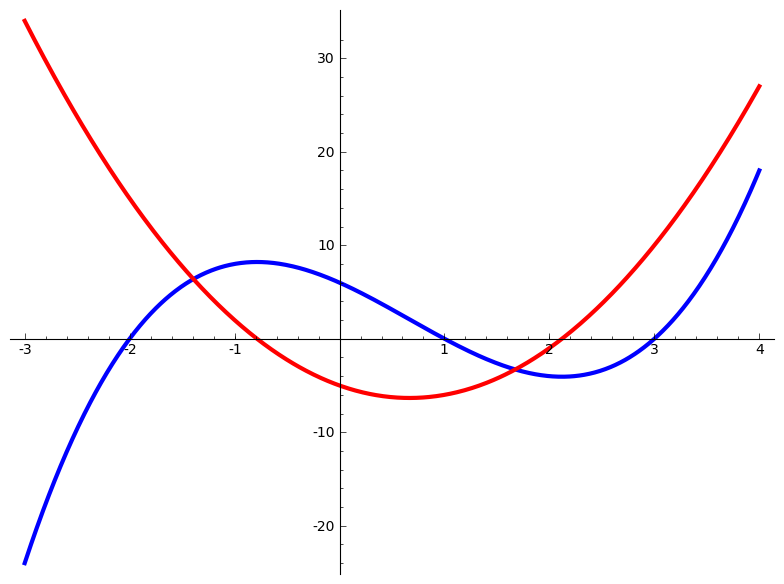
\includegraphics[width=\linewidth]{external/images/cubic-function.png}
\end{image}%
\tcblower
\end{figureptx}%
Lists\footnote{Sixth test footnote\label{section-facts-figures-6-1}} can have multiple columns.  With \initialism{HTML} items displayed in row-major order (horizontally first) and\footnote{Seventh test footnote\label{section-facts-figures-6-3}} with \LaTeX{} items are displayed in column-major order (vertically first).  When one order, or the other, becomes workable in both variants, maybe we will be consistent in presentation.  (Note that with just one row, it makes no difference.)  We used it above for the two items\textemdash{}derivatives and integrals\textemdash{}where each item was a list of its own.  Here are two more examples, one with short snippets and lots of columns, the other with lots of text in paragraphs.\index{list!multicolumn|(}%
\begin{multicols}{5}
\begin{enumerate}
\item{}Red%
\item{}Blue%
\item{}Green%
\item{}Purple%
\item{}Yellow%
\item{}Black%
\item{}Orange%
\item{}Pink%
\item{}Salmon\index{strange colors}%
\item{}Aqua%
\item{}Cyan%
\item{}Puce\index{strange colors}%
\end{enumerate}
\end{multicols}
%
\begin{multicols}{2}
\begin{itemize}[label=\textbullet]
\item{}Lorem ipsum dolor sit amet, consectetur adipiscing elit. Proin lorem diam, convallis in nulla sed, accumsan fermentum urna. Pellentesque aliquet leo elit, ut consequat nunc dapibus ac. Sed lobortis leo tincidunt, vulputate nunc at, ultricies leo. Vivamus purus diam, tristique laoreet purus eget, mollis gravida sapien. Nunc vulputate nisl ac mauris hendrerit cursus. Sed vel molestie velit. Suspendisse sem sem, elementum at vehicula id, volutpat ac mi. Nullam ullamcorper fringilla purus in accumsan. Mauris at nunc accumsan orci dictum vulputate id id augue. Suspendisse at dignissim elit, non euismod nunc. Aliquam faucibus magna ac molestie semper. Aliquam hendrerit sem sit amet metus congue tempor. Donec laoreet laoreet metus, id interdum purus mattis vulputate. Proin condimentum vitae erat varius mollis. Donec venenatis libero sed turpis pretium tempor.%
\par
Praesent rutrum scelerisque felis sit amet adipiscing. Phasellus in mollis velit. Nunc malesuada felis sit amet massa cursus, eget elementum neque viverra. Integer sagittis dictum turpis vel aliquet. Fusce ut suscipit dolor, nec tristique nisl. Aenean luctus, leo et ornare fermentum, nibh dui vulputate leo, nec tincidunt augue ipsum sed odio. Nunc non erat sollicitudin, iaculis eros consequat, dapibus eros.%
\item{}Donec vestibulum auctor nisl. Nullam placerat interdum dui. Quisque lobortis scelerisque augue imperdiet placerat. Maecenas ultricies massa tempor, laoreet urna a, eleifend enim. Integer sed suscipit odio. Pellentesque non dapibus diam, eget tempus dui. Maecenas sollicitudin magna viverra, egestas velit nec, tristique sem. Cras iaculis mattis dui ac cursus. Integer volutpat, urna vel tempus convallis, erat nisi consectetur turpis, id varius dolor lorem vitae mauris. Phasellus erat orci, laoreet commodo gravida quis, congue in lacus. Cum sociis natoque penatibus et magnis dis parturient montes, nascetur ridiculus mus. Praesent at bibendum turpis. Pellentesque est nisl, dapibus at sagittis non, ultricies in nunc. Etiam ipsum arcu, porta sed feugiat eget, facilisis nec libero. Mauris tempor convallis felis.%
\par
Cras iaculis sapien elit, at convallis ligula convallis nec. Duis ante tortor, euismod a libero vitae, ornare viverra purus. Pellentesque facilisis urna a velit volutpat, in malesuada tortor porttitor. Sed vehicula mauris id lectus dignissim, eget consectetur dui pellentesque. Sed vel quam molestie, euismod ligula ac, venenatis arcu. Fusce sit amet sapien non urna dignissim tempus in vitae metus. Aliquam arcu turpis, mattis non libero eu, lacinia feugiat turpis. Phasellus rhoncus lacinia lacus facilisis ullamcorper. Praesent hendrerit accumsan neque, eu dignissim est consequat sed. Nulla facilisi. Proin at mi scelerisque, scelerisque felis ut, tristique diam. Proin in leo in lorem porttitor varius. Praesent condimentum in dui sit amet blandit. In imperdiet blandit congue.%
\item{}Ut nec sem vitae ipsum interdum vestibulum sit amet sed velit. Aliquam tempor nibh vitae augue pulvinar, at ultricies urna commodo. Donec in porta lectus, ac sagittis felis. Vestibulum tincidunt quis metus facilisis luctus. In lobortis lacus vel ornare vehicula. Duis aliquet, ligula semper sodales adipiscing, augue nibh ornare ante, quis pulvinar justo mi eget mi. Mauris varius imperdiet vehicula. Duis dignissim magna quis velit mattis, in cursus lectus vehicula. Morbi quis tempus felis, ut gravida nisi.%
\par
Vivamus eu commodo est, pretium fringilla dolor. Curabitur vel sollicitudin libero. Integer sit amet auctor felis. Maecenas sagittis erat at ante feugiat, in tincidunt ligula pretium. Integer eget auctor ipsum, quis volutpat felis. Morbi id dignissim eros. Suspendisse aliquet pulvinar lorem gravida egestas. Cum sociis natoque penatibus et magnis dis parturient montes, nascetur ridiculus mus. Praesent nec massa dui. Suspendisse convallis lacus sit amet adipiscing varius. Suspendisse tempus diam vitae justo ornare, in condimentum metus pharetra. Curabitur sem dolor, auctor vitae sagittis vestibulum, posuere imperdiet metus. Etiam pretium lacus urna, vel auctor diam tincidunt non. Etiam viverra sodales iaculis.%
\item{}Sed varius leo urna. Phasellus tempus mollis ultricies. Curabitur non neque aliquet, facilisis tortor in, sodales dui. Donec hendrerit ultricies nulla mollis rhoncus. In vel lobortis est. Vestibulum consectetur lacus vel sem dignissim vestibulum. Etiam sed elementum ligula, vel congue turpis. Morbi nec diam mattis, venenatis eros et, elementum tellus. Integer sed orci ornare, elementum elit id, lacinia augue. Vestibulum ante ipsum primis in faucibus orci luctus et ultrices posuere cubilia Curae; In et libero id turpis pharetra faucibus. Integer consequat dignissim semper. Donec pretium magna at ullamcorper ultricies. Nam quis suscipit elit. Donec cursus tellus et venenatis feugiat. Mauris dictum molestie leo, vitae aliquet metus luctus vitae.%
\par
Ut id iaculis leo. Sed nec vestibulum mi. Mauris est mauris, porta in nulla eget, bibendum luctus nisl. Praesent et posuere felis, molestie vehicula velit. Nulla a nunc venenatis, aliquam orci nec, congue felis. Vestibulum a dolor nisi. Morbi sed nisi nulla. Nam iaculis felis a enim blandit, at venenatis diam congue. Nulla augue diam, egestas eget fermentum nec, posuere eget risus. Praesent egestas nulla eros, eget accumsan augue euismod vel. Pellentesque pellentesque non erat vitae posuere. Curabitur lacus arcu, varius sed risus ut, ullamcorper tincidunt lorem. Sed et lacus dignissim, tincidunt nisl ac, porttitor sapien.%
\end{itemize}
\end{multicols}
%
% end of section: Some Facts and Figures
%
%
\typeout{************************************************}
\typeout{Section 6 Some Advanced Ideas}
\typeout{************************************************}
%
\section{Some Advanced Ideas}\label{derivatives-9}%
\index{list!multicolumn|)}The multi-row displayed mathematics in the proof of the Fundamental Theorem had equations aligned on the equals signs via the \& character.  Sometimes you don't want that.  Here is an example with some differential equations, with each equation centered and unnumbered,%
\begin{gather*}
{\mathcal L}(y')(s) = s {\mathcal L}(y)(s) - y(0) = s Y(s) - y(0)\\
{\mathcal L}(y'')(s) = s^2 {\mathcal L}(y)(s) - sy(0) - y'(0)= s^2 Y(s) - sy(0) - y'(0)\text{.}
\end{gather*}
\label{derivatives-9-2-3}\index{rho, a test} Just prior to this sentence, in the middle of this paragraph, is an \mono{<idx>} and a \mono{<notation>}, adjacent, but separated by some whitespace in the authored source.  That insignificant whitespace will be removed akways, which will be a (slightly) noticeable improvement in the \LaTeX{} output.  We test referencing notation here, placed \emph{before} the sentence-ending period and right after some inline mathematics\textemdash{}for \(\mathbb{Z}_n\)\label{derivatives-9-2-11}.%
\par
\LaTeX{} has a device where you can interrupt a sequence of equations with a small amout of text and preserve the equation alignment on either side.  Here are two tests of that device, with aligned equations and non-aligned equations.  Study the source to see use and differences.  (The math does not make sense.)%
\par
Aligned and numbered first.%
\begin{align}
{\mathcal L}(y')(s)  &= s {\mathcal L}(y)(s) - y(0) = s Y(s) - y(0)\label{derivatives-9-4-1-1}\\
{\mathcal L}(y'')(s) &= s^2 {\mathcal L}(y)(s) - sy(0) - y'(0)= s^2 Y(s) - sy(0) - y'(0).\label{derivatives-9-4-1-2}\\
\intertext{And so it follows that,}
{\mathcal L}(y')(s)^{++}  &= s {\mathcal L}(y)(s) - y(0) = s Y(s) - y(0)\label{derivatives-9-4-1-4}\\
{\mathcal L}(y'')(s)^{5} &= s^2 {\mathcal L}(y)(s) - sy(0) - y'(0)= s^2 Y(s) - sy(0) - y'(0).\label{derivatives-9-4-1-5}
\end{align}
%
\par
Now with no numbers and no alignment.  We include two cross-references in the \mono{intertext} portion for testing.%
\begin{gather*}
{\mathcal L}(y')(s)  = s {\mathcal L}(y)(s) - y(0) = s Y(s) - y(0)\\
{\mathcal L}(y'')(s) = s^2 {\mathcal L}(y)(s) - sy(0) - y'(0)= s^2 Y(s) - sy(0) - y'(0).\\
\intertext{First an external reference to \href{http://example.com}{\nolinkurl{example.com}} and internal cross-reference to \hyperref[corollary-FTC-derivative]{Corollary~{\xreffont\ref{corollary-FTC-derivative}}}. And so it follows that,}
{\mathcal L}(y')(s)^{++} = s {\mathcal L}(y)(s) - y(0) = s Y(s) - y(0)\\
{\mathcal L}(y'')(s)^{5} = s^2 {\mathcal L}(y)(s) - sy(0) - y'(0)= s^2 Y(s) - sy(0) - y'(0)\text{.}
\end{gather*}
%
\par
Tables can get quite complex.  Simple ones are simpler, such as this example of numerical computations for Euler's method in just a bit.%
\par
But first we make a figure with two very simple tables next to each other.  This causes the very first instance of \mono{<table>} to actually be a ``subtable'', which exposes a bug provoked by Emiliano Vega and fixed around 2020-08-06. (So we have to place this early to create the same behavior that exposed the bug.)%
\begin{figureptx}{Figure}{Buggy sub-tables}{derivatives-9-8}{}%
\begin{sidebyside}{2}{0}{0}{0}%
\begin{sbspanel}{0.5}%
\begin{subtableptx}{Table}{\textbf{First}}{derivatives-9-8-2-1}{}%
\noindent\resizebox{\ifdim\width > \linewidth\linewidth\else\width\fi}{!}{%
{\centering%
{\tabularfont%
\begin{tabular}{l}
One
\end{tabular}
}%
\par}
}%
\tcblower
\end{subtableptx}%
\end{sbspanel}%
\begin{sbspanel}{0.5}%
\begin{subtableptx}{Table}{\textbf{Second}}{derivatives-9-8-2-2}{}%
\noindent\resizebox{\ifdim\width > \linewidth\linewidth\else\width\fi}{!}{%
{\centering%
{\tabularfont%
\begin{tabular}{l}
Two
\end{tabular}
}%
\par}
}%
\tcblower
\end{subtableptx}%
\end{sbspanel}%
\end{sidebyside}%
\tcblower
\end{figureptx}%
\begin{tableptx}{Table}{\textbf{Euler's approximation for Duffing's Equation with \(h = 0.2\)}}{table-euler1}{}%
\centering%
{\tabularfont%
\begin{tabular}{cccc}\hrulethick
\(i\)&\(t_i\)&\(x_i\)&\(y_i\)\tabularnewline\hrulethin
0&0.00&0.0000&0.5000\tabularnewline[0pt]
1&0.20&0.1000&0.4800\tabularnewline[0pt]
2&0.40&0.1960&0.4560\tabularnewline[0pt]
3&0.60&0.2872&0.4295\tabularnewline[0pt]
4&0.80&0.3731&0.4027\tabularnewline[0pt]
5&1.00&0.4536&0.3783\tabularnewline[0pt]
6&1.20&0.5293&0.3591\tabularnewline[0pt]
7&1.40&0.6011&0.3480\tabularnewline[0pt]
8&1.60&0.6707&0.3474\tabularnewline[0pt]
9&1.80&0.7402&0.3603\tabularnewline[0pt]
10&2.00&0.8123&0.3900\tabularnewline\hrulemedium
\end{tabular}
}%
\end{tableptx}%
% end of section: Some Advanced Ideas
%
%
\typeout{************************************************}
\typeout{Section 7 Mathematics}
\typeout{************************************************}
%
\section{Mathematics}\label{section-mathematics}%
% Introduction
To be able to create both \LaTeX{} and HTML output (plus variations), we rely on MathJax, which in turn supports an extensive subset of the mathematical symbols normally available.  The AMSMath symbol set is a good approximation.  The PreTeXt Guide has a link to the complete list of macros supported by MathJax.  We load the \mono{AMSsymbols} library.%
% end of introduction
%
%
\typeout{************************************************}
\typeout{Subsection 7.1 Basic Mathematics}
\typeout{************************************************}
%
\subsection{Basic Mathematics}\label{section-mathematics-3}%
The following is from the MathJax \href{http://www.mathjax.org/demos/tex-samples/}{demonstration page}\footnote{\nolinkurl{www.mathjax.org/demos/tex-samples/}\label{section-mathematics-3-2-2}}, an identity due to Ramanujan:%
\begin{equation*}
\frac{1}{\Bigl(\sqrt{\phi \sqrt{5}}-\phi\Bigr) e^{\frac25 \pi}} = 1+\frac{e^{-2\pi}} {1+\frac{e^{-4\pi}} {1+\frac{e^{-6\pi}} {1+\frac{e^{-8\pi}} {1+\ldots} } } }
\end{equation*}
%
\par
And again, from the MathJax demonstration page, Maxwell's equations:\index{Maxwell's equations}%
\begin{align*}
\nabla \times \vec{\mathbf{B}} -\, \frac1c\, \frac{\partial\vec{\mathbf{E}}}{\partial t} & = \frac{4\pi}{c}\vec{\mathbf{j}}\\
\nabla \cdot \vec{\mathbf{E}} & = 4 \pi \rho\\
\nabla \times \vec{\mathbf{E}}\, +\, \frac1c\, \frac{\partial\vec{\mathbf{B}}}{\partial t} & = \vec{\mathbf{0}}\\
\nabla \cdot \vec{\mathbf{B}} & = 0
\end{align*}
\label{section-mathematics-3-3-3}%
\par
Historically, we provided internal support for the \LaTeX{} package \mono{extpfeil}.  As of 2023-10-19 this has become an author election (see the \mono{<docinfo>} section in the source of this document).  We preeserve a small test that this extensible arrows library is being included properly:%
\begin{equation*}
A\xmapsto[\text{bijection}]{\Phi+\Psi+\Theta}B
\end{equation*}
%
\par
Look back at the top of the source file of this document to see how to include your \TeX{} macros just once.  For best results keep your macros simple and semantic.%
\par
PreTeXt once provided modest built-in support for ``slanted'', or ``beveled'', or ``nice'' fractions.  To wit, we mean fractions such as: \(\sfrac{3}{8}\).  Use the pre-defined \mono{\textbackslash{}sfrac\{\}\{\}} macro in your mathematics to achieve this presentation.  The presentation in HTML is subpar, but could improve as MathJax provides support.  It is now an author's responsibility to add support for superior typesetting for \initialism{PDF} output by loading the \mono{xfrac} \LaTeX{} package with the following in \mono{<docinfo>}:%
\begin{codedisplay}
<math-package latex-name="xfrac" mathjax-name=""/>
\end{codedisplay}
which is what we have done here as a test.  See the Guide for more details.%
\par
We consider a system of equations.  We number the first and last equation (there are just two) and include an \mono{xml:id} on each.  We reference the whole system later as the range of equations from the first to the last.%
\begin{align}
\frac{dx}{dt} \amp = x^2 - 4x - y + 4\label{equation-system-begin}\\
\frac{dy}{dt} \amp = x^3 - y.\label{equation-system-end}
\end{align}
%
% end of subsection: Basic Mathematics
%
%
\typeout{************************************************}
\typeout{Subsection 7.2 Displayed Mathematics}
\typeout{************************************************}
%
\subsection{Displayed Mathematics}\label{section-mathematics-4}%
Multi-line displays of mathematics are achieved with the \mono{md} tag (``math display''), and the variant that produces numbers on each line, \mono{mdn} (``math display numbered''), used within a paragraph (\mono{p}).  As a good example of how XML syntax is superior, you author \(n\) lines of equations by enclosing each line inside of a \mono{mrow} tag, rather than using \(n-1\) separators (such as \mono{\textbackslash{}\textbackslash{}}).%
\par
If you use no ampersands to express alignment (read ahead), then each equation is centered independently on the width of the text.  This is implemented according to the AMSmath \LaTeX{} package's \mono{gather} environment.  Example:%
\begin{gather*}
\frac{dx}{dt} = x^2 - 4x - y + 4\\
\frac{dy}{dt} = x^3 - y.
\end{gather*}
%
\par
An ampersand is used, in two ways, to describe positioning several equations per line, organized in columns.  We have created the pre-defined \LaTeX{} macro \mono{\textbackslash{}amp} as one way specify these, but the escape sequence \mono{\&amp;} may be used also.  The second, fourth, sixth, \textellipsis{} ampersands separate columns, and the spacing between columns will be provided automatically.  The first, third, fifth, \textellipsis{} ampersands are alignment points for the equations in each column.  Typically this is placed just prior to a binary operator, such as an equal sign (\mono{\textbackslash{}amp = }), or for a column of explanations or commentary, just prior to the \mono{\textbackslash{}text\{\}} macro.  Note that this scenario suggests always having an odd number of ampersands in each \mono{mrow}.  In the example below, alignment is on the equals sign in the first two columns, and provides left-justification to the explanations in the third column.  N.B.: the use below of the \mono{\textbackslash{}text\{\}} macro does not include mathematics within its argument.  Doing so may yield unpredictable results depending on your choice of delimiters for the mathematics (and using an \mono{m} tag will be ineffective).%
\begin{align*}
\frac{dx}{dt} \amp = x^2 - 4x - y + 4 \amp \frac{dy}{dt} \amp = x^3 - y          \amp\amp x, y\text{ version}\\
\frac{dw}{dt} \amp = z^3 - w          \amp \frac{dz}{dt} \amp = z^2 - 4z - w + 4 \amp\amp z, w\text{ version}
\end{align*}
%
\par
PreTeXt will automatically detect the presence or absence of ampersands, but by defining macros for entire aligned equations, you can effectively hide the ampersands.  So the \mono{@alignment} attribute can override automatic detection.  We use a simple \LaTeX{} macro to demonstrate setting \mono{alignment=\textquotesingle{}align\textquotesingle{}} to override the use of a \mono{gather} environment and use a \mono{align} environment instead.  Example:%
\begin{align*}
\myequation{\frac{dx}{dt}}{x^2 - 4x - y + 4}\\
\myequation{\frac{dy}{dt}}{x^3 - y}.
\end{align*}
%
\par
The AMSmath \LaTeX{} package's \mono{alignat} environment is a third variant of alignment.  It never happens automatically, you need to ask for it with \mono{alignment=\textquotedbl{}alignat\textquotedbl{}}.  It is very similar to \mono{align} but adds no space between the equation columns.  So you can leave it that way, or you can add your own ``extra'' space to suit.  Here is a previous example with no inter-column space:%
\begin{alignat*}{3}
\frac{dx}{dt} \amp = x^2 - 4x - y + 4 \amp \frac{dy}{dt} \amp = x^3 - y          \amp\amp x, y\text{ version}\\
\frac{dw}{dt} \amp = z^3 - w          \amp \frac{dz}{dt} \amp = z^2 - 4z - w + 4 \amp\amp z, w\text{ version}\text{.}
\end{alignat*}
This modified example has a middle row with three columns, while the other rows have just one column, as a test of our routines for determining the \mono{mrow} with the greatest number of ampersands (and how many there are),%
\begin{alignat*}{3}
\frac{dw}{dt} &= z^3 - w\\
\frac{dx}{dt} &= x^2 - 4x - y + 4 & \frac{dy}{dt} &= x^3 - y&& x, y\text{ third column}\\
\frac{dw}{dt} & = z^3 - w\text{.}
\end{alignat*}
Final example demonstrates that ampersands in other objects (matrices here) can wreak havoc with computing the number of columns.  So we provide yet another attribute to override automatic detection, \mono{alignat-columns}.  This is the number of \emph{columns} not the number of \emph{ampersands}.  Generally, for \(c\) columns, there will be \(2c-1\) ampersands.%
\begin{alignat*}{2}
A &= \begin{bmatrix}1 & 2 \\ 3 & 4\end{bmatrix}
&
I &= \begin{bmatrix}1 & 0 \\ 0 & 1\end{bmatrix}\text{.}
\end{alignat*}
One caveat: if your number of ampersands is even (see advice above about using an odd number) behavior should still be correct, as in next example.%
\par
If you want super-precise control over alignment of the terms of a system of equations (linear or not) you can use the \mono{alignat} option to advantage by not including any extra space.  This example is modified slightly from a post by Alex Jordan:%
\begin{alignat*}{4}
2x \amp {}+{} \amp  y \amp {}+{} \amp 3z \amp {}={} \amp 10\\
x  \amp       \amp    \amp {}+{} \amp  z \amp {}={} \amp 6\\
x  \amp {}+{} \amp 3y \amp {}+{} \amp 2z \amp {}={} \amp 13.
\end{alignat*}
Beautiful.%
\par
A long equation, to check layout on various screen sizes.  This is Weil's ``explicit formula'' for the Riemann \(\zeta\)-function:%
\begin{equation}
\sum_\gamma S_-(\gamma) = \frac{\log Q}{\pi} \hat S_-(0)
+ \frac{1}{2\pi} \sum_{j=1}^d \Re\left\{ \int_{-\infty}^\infty \frac{\Gamma'}{\Gamma}\left(\frac{1}{4} + \frac{it}{2} + \mu_j\right)S_-(t) dt\right\}
- \frac{d}{2\pi}\hat S_-(0)\log \pi\text{.}\label{section-mathematics-4-8-3}
\end{equation}
%
\begin{example}[Excessive Display Mathematics]\label{section-mathematics-4-9}%
%
In print versions, a long run of displayed equations often needs to be broken across pages.  If you are reading some other version of this, then there is nothing to see here.  But for \LaTeX{} output it could be interesting.  First, with no extra effort, this page-long display should break naturally, no matter how the preceding material changes.%
\begin{gather*}
x^2+y^2=z^2\\
a^2+b^2=c^2\\
\alpha^2+\beta^2=\gamma^2\\
m^2+n^2=p^2\\
x^2+y^2=z^2\\
a^2+b^2=c^2\\
\alpha^2+\beta^2=\gamma^2\\
m^2+n^2=p^2\\
x^2+y^2=z^2\\
a^2+b^2=c^2\\
\alpha^2+\beta^2=\gamma^2\\
m^2+n^2=p^2\\
x^2+y^2=z^2\\
a^2+b^2=c^2\\
\alpha^2+\beta^2=\gamma^2\\
m^2+n^2=p^2\\
x^2+y^2=z^2\\
a^2+b^2=c^2\\
\alpha^2+\beta^2=\gamma^2\\
m^2+n^2=p^2\\
x^2+y^2=z^2\\
a^2+b^2=c^2\\
\alpha^2+\beta^2=\gamma^2\\
m^2+n^2=p^2\\
x^2+y^2=z^2\\
a^2+b^2=c^2\\
\alpha^2+\beta^2=\gamma^2\\
m^2+n^2=p^2\\
x^2+y^2=z^2\\
a^2+b^2=c^2\\
\alpha^2+\beta^2=\gamma^2\\
m^2+n^2=p^2\\
x^2+y^2=z^2\\
a^2+b^2=c^2\\
\alpha^2+\beta^2=\gamma^2\\
m^2+n^2=p^2\\
x^2+y^2=z^2\\
a^2+b^2=c^2\\
\alpha^2+\beta^2=\gamma^2\\
m^2+n^2=p^2\\
x^2+y^2=z^2\\
a^2+b^2=c^2\\
\alpha^2+\beta^2=\gamma^2\\
m^2+n^2=p^2\\
x^2+y^2=z^2\\
a^2+b^2=c^2\\
\alpha^2+\beta^2=\gamma^2\\
m^2+n^2=p^2\text{.}
\end{gather*}
%
\par
In this version we have turned off page breaking for the entire display, but then allowed a break at every fourth equation, so you should see a reasonably attractive page break right after one of the \(m^2+n^2=p^2\) equations.%
\begin{gather}
x^2+y^2=z^2\label{section-mathematics-4-9-3-2-1}\\*
a^2+b^2=c^2\label{section-mathematics-4-9-3-2-2}\\*
\alpha^2+\beta^2=\gamma^2\label{section-mathematics-4-9-3-2-3}\\*
m^2+n^2=p^2\label{section-mathematics-4-9-3-2-4}\\
x^2+y^2=z^2\label{section-mathematics-4-9-3-2-5}\\*
a^2+b^2=c^2\label{section-mathematics-4-9-3-2-6}\\*
\alpha^2+\beta^2=\gamma^2\label{section-mathematics-4-9-3-2-7}\\*
m^2+n^2=p^2\label{section-mathematics-4-9-3-2-8}\\
x^2+y^2=z^2\label{section-mathematics-4-9-3-2-9}\\*
a^2+b^2=c^2\label{section-mathematics-4-9-3-2-10}\\*
\alpha^2+\beta^2=\gamma^2\label{section-mathematics-4-9-3-2-11}\\*
m^2+n^2=p^2\label{section-mathematics-4-9-3-2-12}\\
x^2+y^2=z^2\label{section-mathematics-4-9-3-2-13}\\*
a^2+b^2=c^2\label{section-mathematics-4-9-3-2-14}\\*
\alpha^2+\beta^2=\gamma^2\label{section-mathematics-4-9-3-2-15}\\*
m^2+n^2=p^2\label{section-mathematics-4-9-3-2-16}\\
x^2+y^2=z^2\label{section-mathematics-4-9-3-2-17}\\*
a^2+b^2=c^2\label{section-mathematics-4-9-3-2-18}\\*
\alpha^2+\beta^2=\gamma^2\label{section-mathematics-4-9-3-2-19}\\*
m^2+n^2=p^2\label{section-mathematics-4-9-3-2-20}\\
x^2+y^2=z^2\label{section-mathematics-4-9-3-2-21}\\*
a^2+b^2=c^2\label{section-mathematics-4-9-3-2-22}\\*
\alpha^2+\beta^2=\gamma^2\label{section-mathematics-4-9-3-2-23}\\*
m^2+n^2=p^2\label{section-mathematics-4-9-3-2-24}\\
x^2+y^2=z^2\label{section-mathematics-4-9-3-2-25}\\*
a^2+b^2=c^2\label{section-mathematics-4-9-3-2-26}\\*
\alpha^2+\beta^2=\gamma^2\label{section-mathematics-4-9-3-2-27}\\*
m^2+n^2=p^2\label{section-mathematics-4-9-3-2-28}\\
x^2+y^2=z^2\label{section-mathematics-4-9-3-2-29}\\*
a^2+b^2=c^2\label{section-mathematics-4-9-3-2-30}\\*
\alpha^2+\beta^2=\gamma^2\label{section-mathematics-4-9-3-2-31}\\*
m^2+n^2=p^2\label{section-mathematics-4-9-3-2-32}\\
x^2+y^2=z^2\label{section-mathematics-4-9-3-2-33}\\*
a^2+b^2=c^2\label{section-mathematics-4-9-3-2-34}\\*
\alpha^2+\beta^2=\gamma^2\label{section-mathematics-4-9-3-2-35}\\*
m^2+n^2=p^2\label{section-mathematics-4-9-3-2-36}\\
x^2+y^2=z^2\label{section-mathematics-4-9-3-2-37}\\*
a^2+b^2=c^2\label{section-mathematics-4-9-3-2-38}\\*
\alpha^2+\beta^2=\gamma^2\label{section-mathematics-4-9-3-2-39}\\*
m^2+n^2=p^2\label{section-mathematics-4-9-3-2-40}\\
x^2+y^2=z^2\label{section-mathematics-4-9-3-2-41}\\*
a^2+b^2=c^2\label{section-mathematics-4-9-3-2-42}\\*
\alpha^2+\beta^2=\gamma^2\label{section-mathematics-4-9-3-2-43}\\*
m^2+n^2=p^2\label{section-mathematics-4-9-3-2-44}\\
x^2+y^2=z^2\label{section-mathematics-4-9-3-2-45}\\*
a^2+b^2=c^2\label{section-mathematics-4-9-3-2-46}\\*
\alpha^2+\beta^2=\gamma^2\label{section-mathematics-4-9-3-2-47}\\*
m^2+n^2=p^2\text{.}\label{section-mathematics-4-9-3-2-48}
\end{gather}
%
\par
So.  Do not take any extra steps and let \LaTeX{} figure out the breaks.  If you do not like a break, modify the \mono{md} or \mono{mdn} to go back to the AMSmath default behavior and not break at all.  Ever.  Or rather, go further and modify an individual \mono{mrow} to suggest that it is a good place for a break.%
\end{example}
This is a poorly-authored paragaph to test the conversion to \initialism{HTML}.  There are two displayed equations, separated by a period ending the first one's sentence, which should migrate into the display, and not leave behind an empty paragraph:%
\begin{equation*}
z+y = z\text{.}
\end{equation*}
%
\begin{equation*}
a + b = c\text{.}
\end{equation*}
This final sentence should remain, inside another \initialism{HTML} paragraph, without the second equation's period.%
% end of subsection: Displayed Mathematics
%
%
\typeout{************************************************}
\typeout{Subsection 7.3 \LaTeX{} Packages and MathJax Extensions}
\typeout{************************************************}
%
\subsection{\LaTeX{} Packages and MathJax Extensions}\label{section-mathematics-5}%
If you would like to enhance your mathematics by using a macro from a \LaTeX{} package \emph{and} there is a MathJax extension \emph{which implements the same macro}, then you may use this with your mathematics as we demonstrate here.%
\par
This example is from Jason Underdown.\index{Underdown, Jason}  The package is named \mono{cancel} and is included in the TeXLive distribution, so is fairly standard.  The particular macro being demonstrated is \mono{\textbackslash{}cancelto\{\}\{\}}.%
\begin{equation*}
\lim_{b \rightarrow \infty}\left[\cancelto{0}{-\frac{1}{s}e^{-sb}} + \frac{1}{s}\right]\text{.}
\end{equation*}
Look at the source of this article to see the package name being supplied in a \mono{<math-package>} element within the \mono{<docinfo>} section.  That is the only setup required to make the macro usable in \LaTeX{} and \initialism{HTML} output.\index{canceling a term}\index{cancelto macro@\mono{cancelto} macro}%
\par
See the \pubtitle{PreTeXt Guide} subsection about ``MathJax Extensions'' for more detail.%
% end of subsection: \LaTeX{} Packages and MathJax Extensions
%
%
\typeout{************************************************}
\typeout{Subsection 7.4 Advanced Mathematics}
\typeout{************************************************}
%
\subsection{Advanced Mathematics}\label{section-mathematics-6}%
MathJax is extremely capable in rendering a subset of \LaTeX{} in web browsers, and improving all the time.  You can get fairly fancy with some of its supported commands.  In particular, if you need to mix in a few words with your mathematics, the \mono{\textbackslash{}text\{\}} macro is supported.  For example, you might use an ``if'' or an ``otherwise'' in the definition of a piecewise function.%
\par
Consider that the first line below is text sandwiched in-between two Greek letters, wrapped in a \mono{\textbackslash{}text\{\}} macro.  In HTML output we have taken care that the font for text material within display mathematics should match the font of the  surrounding paragraph, as also happens with \LaTeX{} output.  The second line is nearly identical in the source, but is just naked text being rendered like a slew of variables.%
\begin{gather*}
\alpha\text{ is not equal to }\beta\\
\alpha is not equal to \beta\\
\alpha\neq\beta\text{.}
\end{gather*}
We are not suggesting here that using words in place of symbols, as in the first line, is a good practice.  (It is not.)%
\par
The following example is a good stress-test of using the \mono{\textbackslash{}text\{\}} macro to achieve certain effects.  Note the Unicode left and right smart quotes.  This a contribution from Alex Jordan as part of his work on \pubtitle{APEX Calculus}.%
\begin{gather*}
y \rightarrow \frac{\sin(0) }{0} \rightarrow {{\text{“}}\atop{}}\frac{0}{0}{{\text{”}}\atop{}}\text{.}
\end{gather*}
And another one from Alex.  Note the use of the \mono{\textbackslash{}mathord\{\}} and \mono{\textbackslash{}mathrel\{\}} macros to control spacing around the mathematical symbols.  Examine the source to see how the quotation marks have been authored with \initialism{XML} syntax for Unicode characters, since we do not allow most markup inside mathematics.%
\begin{gather*}
\zeta(1)=\sum_{n=1}^{\infty}\frac{1}{n}\mathrel{\text{ “}\mathord{=}{\text{” }}}\prod_{p}\left(\frac{1}{1-1/p}\right)=\prod_{p}\left(\frac{1}{1-p^{-1}}\right)
\end{gather*}
%
\par
Generally, you cannot use any \initialism{XML} elements inside of the mathematics elements.  An exception is the \mono{xref} element which you might want to use to provide justifications for the steps of a derivation.  Here is a visual example that is mathematically meaningless,%
\begin{align*}
A&=B+C&&\hyperref[corollary-FTC-derivative]{\text{Corollary {\xreffont\ref{corollary-FTC-derivative}}}}\\
&=D+E&&\hyperref[theorem-FTC]{\text{The Fundamental Theorem of Calculus}}\\
&=F+G&&\hyperref[theorem-number-01]{\text{A nice result}}\text{.}
\end{align*}
%
\par
Scott Beaver likes to write short chains of equalities all in one line, with the cross-references sitting on each equals sign.  Here we test the \LaTeX{} \mono{\textbackslash{}overset} and \mono{\textbackslash{}underset} macros wrapping a PreTeXt \mono{<xref>}, with and without content, inside an \mono{<me>} element.  Note that  \mono{\textbackslash{}stackrel} is obsolete, and \mono{\textbackslash{}overunderset} is not yet supported by MathJax (but see \href{https://github.com/mathjax/MathJax/issues/2704}{GitHub \#2704}\footnote{\nolinkurl{github.com/mathjax/MathJax/issues/2704}\label{section-mathematics-6-6-10}}).  The mathematics is Scott's, the reasons are totally unrelated to the math.%
\begin{equation*}
AC-AD
\overset{\hyperref[theorem-FTC]{{\xreffont\ref{theorem-FTC}}}}{=}
A(C-D)
\underset{\hyperref[definition-indefinite-integral]{{\xreffont\ref{definition-indefinite-integral}}}}{=}
A0_{n\times p}
\overset{\hyperref[theorem-FTC]{Thm.~{\xreffont\ref{theorem-FTC}}}}{=}
0_{m\times p}
\end{equation*}
We suggest using cross-references that only display numbers (\mono{<xref>} with \mono{@text} set to \mono{global}) since if you stick to elements like \mono{<theorem>}, \mono{<lemma>}, \mono{<definition>}, or \mono{<axiom>}, then the numbers will be unambiguous and the target of the cross-reference will contain full information.  But note that if you mix in divisions, or perhaps figures, as reasons then there is a possibility that numbers will need to be qualified by their type.  We have provided an abbreviation for one cross-reference to \hyperref[theorem-FTC]{Theorem~{\xreffont\ref{theorem-FTC}}} (which will not benefit from automatic translation to other languages).%
% end of subsection: Advanced Mathematics
%
%
\typeout{************************************************}
\typeout{Subsection 7.5 Local Tags on Equations}
\typeout{************************************************}
%
\subsection{Local Tags on Equations}\label{section-mathematics-7}%
If you are not writing a research monograph, maybe (a) you will not use many numbered equations, or do not like the looks of them, or feel they scare your readers, and (b) maybe your cross-references are always local-ish, like strictly within an \mono{example} or a \mono{proof}.  For this situation you can create, and employ, a ``local'' tag on a displayed equation.  Nothing enforces the idea of what constitutes local, and there is nothing to stop you from using the same symbols more than once.  With freedom comes responsibility.%
\par
Use the \mono{@tag} attribute on an \mono{mrow}, only.  (Remember, you can have just one \mono{mrow}.)  The behavior is identical within an \mono{md} or \mono{mdn}.  The value of the \mono{@tag} attribute is a symbol name.  The prefix \mono{d} means ``double'', and the prefix \mono{t} means ``triple''.  So allowed values are%
\begin{codedisplay}
star, dstar, tstar
dagger, ddagger, tdagger
daggerdbl, ddaggerdbl, tdaggerdbl
hash, dhash, thash
maltese, dmaltese, tmaltese
\end{codedisplay}
Cross-references to these tagged equations happens in the usual way and should behave as expected.  We test the double versions to make sure the symbols render properly in various output formats.%
\begin{align}
c^2 \amp = a^2+b^2\tag{\textasteriskcentered\textasteriskcentered}\label{equation-local-star}\\
c^2 \amp = a^2+b^2\tag{\textdagger\textdagger}\label{equation-local-dagger}\\
c^2 \amp = a^2+b^2\tag{\textdaggerdbl\textdaggerdbl}\label{equation-local-daggerdbl}\\
c^2 \amp = a^2+b^2\tag{\#\#}\label{equation-local-hash}\\
c^2 \amp = a^2+b^2\tag{\maltese\maltese}\label{equation-local-maltese}\\
z^2 \amp = x^2+y^2\label{section-mathematics-7-3-12-6}
\end{align}
Here are the local cross-references: \hyperref[equation-local-star]{({\xreffont\ref{equation-local-star}})}, \hyperref[equation-local-dagger]{({\xreffont\ref{equation-local-dagger}})}, \hyperref[equation-local-daggerdbl]{({\xreffont\ref{equation-local-daggerdbl}})}, \hyperref[equation-local-hash]{({\xreffont\ref{equation-local-hash}})}, \hyperref[equation-local-maltese]{({\xreffont\ref{equation-local-maltese}})}.  We test another farther away in \hyperref[section-cross-referencing]{Section~{\xreffont\ref{section-cross-referencing}}}, contrary to our advice above.%
% end of subsection: Local Tags on Equations
%
%
\typeout{************************************************}
\typeout{Subsection 7.6 Commutative Diagrams}
\typeout{************************************************}
%
\subsection{Commutative Diagrams}\label{commutative-diagrams}%
This diagram is authored by Tom Judson using the syntax of the \initialism{AMS} \LaTeX{} ``CD'' package.  Inside of a \mono{<me>} element start with \mono{\textbackslash{}begin\{CD\}}.  Remember to escape the less-than character.%
\begin{equation*}
\begin{CD}
E[x]/\langle p(x) \rangle    @>\psi>>  F[x]/\langle q(x) \rangle\\
@VV{\sigma}V        @VV{\tau}V\\
E(\alpha)     @>\overline{\phi}>>  F(\beta)\\
@VVV        @VVV\\
E     @>\phi>>  F
\end{CD}
\end{equation*}
While this package is not as flexible as some generic drawing packages, it has the advantage of full support by MathJax, and thus the \initialism{HTML} version will be more accessible.%
% end of subsection: Commutative Diagrams
%
%
\typeout{************************************************}
\typeout{Subsection 7.7 Line-Breaking after Mathematics}
\typeout{************************************************}
%
\subsection{Line-Breaking after Mathematics}\label{line-breaking-math}%
As of 2021-05-14, in \initialism{HTML} output the next sentence should just fill a full line across the page.  We take active measures to bind the concluding period to the final bit of mathematics, the variable \(x\).  The prevents a bad line break which could see the period \emph{begin} a new line, all by itself.  In the event that the line-breaking siutation improves, we could relax these measures.  This testing is only relevant to \initialism{HTML} output, not \LaTeX{} output.%
\par
xxx xxx xxx xxx xxx xxx xxx xxx xxx xxx xxx xxx xxx xxx xxx xxx xxx xxx xxx xxx \(x\).%
% end of subsection: Line-Breaking after Mathematics
%
%
\typeout{************************************************}
\typeout{Subsection 7.8 Fonts and Mathematics}
\typeout{************************************************}
%
\subsection{Fonts and Mathematics}\label{font-math}%
This section is about testing types and sizes of fonts, not so much about using different typefaces.  First, one long displayed equation, which is designed to be full-width for \LaTeX{} output when using defaults as of 2020-01-29 (commit \mono{defd4bffd462e7ea}).%
\par
Start paragraph.%
\begin{equation*}
a^2 + b^2 + a^2 + b^2 + a^2 + b^2 + a^2 + b^2 + a^2 + b^2 + a^2 + b^2 + a^2 + b^2 + a^2 + b^2 + a^2 + b^2 + a^2 + b^2
\end{equation*}
End paragraph.%
\par
The next paragraph has five ways to write the sine of \(x\), bracketed by plain text versions.  This tests font size and the fonts employed.  The raw source of this paragraph is (spread over two lines)%
\begin{codedisplay}
sin x | <m>\sin x</m> | <m>\text{sin}\ x</m> | <m>\mathrm{sin}\ x</m> |
<m>\text{sin}x</m> | <m>sin x</m> | sin x
\end{codedisplay}
The five ways, from good to bad,%
\begin{enumerate}
\item{}The best way, using  \mono{\textbackslash{}sin}.  Note the distance to the \(x\).%
\item{}With a \mono{\textbackslash{}text\{\}} macro.%
\item{}With a \mono{\textbackslash{}mathrm\{\}} macro.  Not recommended for PreTeXt.%
\item{}Without a space.  Note that the previous two require explicit spacing.%
\item{}No extra effort, so \LaTeX{} renders as a product of four variables.%
\end{enumerate}
%
\par
sin x \textbar{} \(\sin x\) \textbar{} \(\text{sin}\ x\) \textbar{} \(\mathrm{sin}\ x\)  \textbar{} \(\text{sin}x\) \textbar{} \(sin x\) \textbar{} sin x%
\par
Finally a simple paragraph that places a text ``x'' next to a variable ``x''.%
\par
wordxx\(x+x\)xxword%
% end of subsection: Fonts and Mathematics
%
%
\typeout{************************************************}
\typeout{Subsection 7.9 Miscellaneous}
\typeout{************************************************}
%
\subsection{Miscellaneous}\label{miscellaneous-math}%
In \initialism{HTML} output, a MathJax workaround for a Safari rendering bug was inserting extra spaces after textual subscripts and superscripts (\href{https://groups.google.com/g/mathjax-users/c/ANjLK9KtcWA/m/vlHaPja-AwAJ}{MathJax thread}\footnote{\nolinkurl{groups.google.com/g/mathjax-users/c/ANjLK9KtcWA/m/vlHaPja-AwAJ}\label{miscellaneous-math-2-3}}).  PreTeXt CSS now applies a correction.  The following tests if the CSS fix is sufficient, and could be used to test the necessity of our fix in the future.  Following is the original report, though \mono{NOT} has been moved to a superscript:%
\begin{gather*}
T_\text{clk}-t_\text{su} \gt t_\text{clk-Q} + \max\left( t_\text{XOR}, t^\text{NOT} \right)\text{.}
\end{gather*}
There should not be anything to see in \LaTeX{}\slash{}\initialism{PDF} output. (2021-10-21)%
% end of subsection: Miscellaneous
% end of section: Mathematics
%
%
\typeout{************************************************}
\typeout{Section 8 Grouping Samples}
\typeout{************************************************}
%
\section{Grouping Samples}\label{block-samples}%
% Introduction
While building or testing a rendering of PreTeXt, especially in HTML, it can be useful to see all the various elements that potentially create visual blocks in one place. So they are collected here.%
\par
We will omit content specific blocks like figures, images, tables, etc.\@ as those elements have significant stress testing of their own elsewhere.%
\par
Please add any similar elements that are created or that you discover are missing from this page.%
\begin{aside}[A title.]\label{block-samples-2-4}%
%
There are more \mono{<aside>}es below, but here is a solor one.%
\end{aside}
% end of introduction
\begin{objectives}{Objectives: Our goals}{block-samples-3}
%
\begin{itemize}[label=\textbullet]
\item{}Stress test HTML themes%
\item{}Locally, test objectives%
\end{itemize}
\end{objectives}
%
%
\typeout{************************************************}
\typeout{Subsection 8.1 Remark-like Blocks}
\typeout{************************************************}
%
\subsection{Remark-like Blocks}\label{block-samples-remark-like}%
\begin{remark}[A title]\label{block-samples-remark-like-2}%
%
A minimal \mono{<remark>}.%
\end{remark}
\begin{convention}[A title]\label{block-samples-remark-like-3}%
%
A minimal \mono{<convention>}.%
\end{convention}
\begin{note}[A title]\label{block-samples-remark-like-4}%
%
A minimal \mono{<note>}.%
\end{note}
\begin{observation}[A title]\label{block-samples-remark-like-5}%
%
A minimal \mono{<observation>}.%
\end{observation}
\begin{warning}[A title]\label{block-samples-remark-like-6}%
%
A minimal \mono{<warning>}.%
\end{warning}
\begin{insight}[A title]\label{block-samples-remark-like-7}%
%
A minimal \mono{<insight>}.%
\end{insight}
% end of subsection: Remark-like Blocks
%
%
\typeout{************************************************}
\typeout{Subsection 8.2 Example-like Blocks}
\typeout{************************************************}
%
\subsection{Example-like Blocks}\label{block-samples-example-like}%
\begin{example}[A title]\label{block-samples-example-like-2}%
%
A minimal \mono{<example>}.%
\end{example}
\begin{example}[A title]\label{block-samples-example-like-3}%
%
A structured \mono{<example>}.%
\begin{enumerate}[font=\bfseries,label=(\alph*),ref=\alph*]%
\item{}A structured \mono{<example>}.%
\par\smallskip%
\noindent\textbf{\blocktitlefont Hint}.\hypertarget{block-samples-example-like-3-3-2}{}\quad{}A \mono{<hint>}%
\par\smallskip%
\noindent\textbf{\blocktitlefont Answer}.\hypertarget{block-samples-example-like-3-3-3}{}\quad{}An \mono{<answer>}%
\par\smallskip%
\noindent\textbf{\blocktitlefont Solution}.\hypertarget{block-samples-example-like-3-3-4}{}\quad{}A \mono{<solution>}%
\end{enumerate}%
The \mono{<conclusion>}.%
\end{example}
\begin{question}[A title]\label{block-samples-example-like-4}%
%
A minimal \mono{<question>}.%
\end{question}
\begin{problem}[A title]\label{block-samples-example-like-5}%
%
A minimal \mono{<problem>}.%
\end{problem}
\begin{observation}[A title]\label{block-samples-example-like-6}%
%
A minimal \mono{<observation>}.%
\end{observation}
\begin{warning}[A title]\label{block-samples-example-like-7}%
%
A minimal \mono{<warning>}.%
\end{warning}
\begin{insight}[A title]\label{block-samples-example-like-8}%
%
A minimal \mono{<insight>}.%
\end{insight}
% end of subsection: Example-like Blocks
%
%
\typeout{************************************************}
\typeout{Subsection 8.3 Theorem-like Blocks}
\typeout{************************************************}
%
\subsection{Theorem-like Blocks}\label{block-samples-theorem-like}%
\begin{theorem}[A title]\label{block-samples-theorem-like-2}%
%
A minimal \mono{<theorem>}.%
\end{theorem}
\begin{theorem}[A title]\label{block-samples-theorem-like-3}%
%
A theorem with a proof.%
\end{theorem}
\begin{proof}\label{block-samples-theorem-like-3-3}%
The proof of the theorem.%
\end{proof}
\begin{corollary}[A title]\label{block-samples-theorem-like-4}%
%
A minimal \mono{<corollary>}.%
\end{corollary}
\begin{lemma}[A title]\label{block-samples-theorem-like-5}%
%
A minimal \mono{<lemma>}.%
\end{lemma}
\begin{algorithm}[A title]\label{block-samples-theorem-like-6}%
%
A minimal \mono{<algorithm>}.%
\end{algorithm}
\begin{proposition}[A title]\label{block-samples-theorem-like-7}%
%
A minimal \mono{<proposition>}.%
\end{proposition}
\begin{claim}[A title]\label{block-samples-theorem-like-8}%
%
A minimal \mono{<claim>}.%
\end{claim}
\begin{fact}[A title]\label{block-samples-theorem-like-9}%
%
A minimal \mono{<fact>}.%
\end{fact}
\begin{identity}[A title]\label{block-samples-theorem-like-10}%
%
A minimal \mono{<identity>}.%
\end{identity}
\begin{proof}[A title]\label{block-samples-theorem-like-11}%
A stand-alone proof.%
\end{proof}
% end of subsection: Theorem-like Blocks
%
%
\typeout{************************************************}
\typeout{Subsection 8.4 Axiom-like Blocks}
\typeout{************************************************}
%
\subsection{Axiom-like Blocks}\label{block-samples-axiom-like}%
\begin{axiom}[A title]\label{block-samples-axiom-like-2}%
%
A minimal \mono{<axiom>}.%
\end{axiom}
\begin{conjecture}[A title]\label{block-samples-axiom-like-3}%
%
A minimal \mono{<conjecture>}.%
\end{conjecture}
\begin{principle}[A title]\label{block-samples-axiom-like-4}%
%
A minimal \mono{<principle>}.%
\end{principle}
\begin{heuristic}[A title]\label{block-samples-axiom-like-5}%
%
A minimal \mono{<heuristic>}.%
\end{heuristic}
\begin{hypothesis}[A title]\label{block-samples-axiom-like-6}%
%
A minimal \mono{<hypothesis>}.%
\end{hypothesis}
\begin{assumption}[A title]\label{block-samples-axiom-like-7}%
%
A minimal \mono{<assumption>}.%
\end{assumption}
% end of subsection: Axiom-like Blocks
%
%
\typeout{************************************************}
\typeout{Subsection 8.5 Definition-like Blocks}
\typeout{************************************************}
%
\subsection{Definition-like Blocks}\label{block-samples-definition-like}%
\begin{definition}[A title]\label{block-samples-definition-like-2}%
%
A minimal \mono{<definition>}.%
\end{definition}
% end of subsection: Definition-like Blocks
%
%
\typeout{************************************************}
\typeout{Subsection 8.6 Aside-like Blocks}
\typeout{************************************************}
%
\subsection{Aside-like Blocks}\label{block-samples-aside-like}%
Three \mono{<aside>}s are below.%
\begin{aside}[A title.]\label{block-samples-aside-like-3}%
%
A minimal \mono{<aside>}.%
\end{aside}
\begin{biographical}[A title.]\label{block-samples-aside-like-4}%
%
A minimal \mono{<biographical>}.%
\end{biographical}
\begin{biographical}[A title.]\label{block-samples-aside-like-5}%
%
A minimal \mono{<biographical>}.%
\end{biographical}
\begin{historical}[A title.]\label{block-samples-aside-like-6}%
%
A minimal \mono{<historical>}.%
\end{historical}
% end of subsection: Aside-like Blocks
%
%
\typeout{************************************************}
\typeout{Subsection 8.7 Computation-like Blocks}
\typeout{************************************************}
%
\subsection{Computation-like Blocks}\label{block-samples-computation-like}%
\begin{computation}[A title]\label{block-samples-computation-like-2}%
%
A minimal \mono{<computation>}.%
\end{computation}
\begin{technology}[A title]\label{block-samples-computation-like-3}%
%
A minimal \mono{<technology>}.%
\end{technology}
\begin{data}[A title]\label{block-samples-computation-like-4}%
%
A minimal \mono{<data>}.%
\end{data}
% end of subsection: Computation-like Blocks
%
%
\typeout{************************************************}
\typeout{Subsection 8.8 Project-like Blocks}
\typeout{************************************************}
%
\subsection{Project-like Blocks}\label{block-samples-project-like}%
\begin{project}[A title]\label{block-samples-project-like-2}%
%
A minimal \mono{<project>}.%
\end{project}%
\begin{activity}[A title]\label{block-samples-project-like-3}%
%
A minimal \mono{<activity>}.%
\end{activity}%
\begin{exploration}[A title]\label{block-samples-project-like-4}%
%
A minimal \mono{<exploration>}.%
\end{exploration}%
\begin{investigation}[A title]\label{block-samples-project-like-5}%
%
A minimal \mono{<investigation>}.%
\end{investigation}%
% end of subsection: Project-like Blocks
\begin{assemblage}\label{block-samples-12}%
%
A minimal \mono{<assemblage>}.%
\end{assemblage}
% Conclusion
A minimal \mono{<conclusion>}.%
% end of conclusion
\begin{aside}[A title.]\label{block-samples-14}%
%
A final \mono{<aside>} to test behavior at the end of a page. Lorem ipsum dolor sit amet, consectetur adipiscing elit, sed do eiusmod tempor incididunt ut labore et dolore magna aliqua. Ut enim ad minim veniam, quis nostrud exercitation ullamco laboris nisi ut aliquip ex ea commodo consequat. Duis aute irure dolor in reprehenderit in voluptate velit esse cillum dolore eu fugiat nulla pariatur. Excepteur sint occaecat cupidatat non proident, sunt in culpa qui officia deserunt mollit anim id est laborum.%
\end{aside}
% end of section: Grouping Samples
%
%
\typeout{************************************************}
\typeout{Section 9 Entering Text in Paragraphs, Titles, Captions}
\typeout{************************************************}
%
\section{Entering Text in Paragraphs, Titles, Captions}\label{section-text-paragraphs}%
% Introduction
\initialism{XML}, and therefore PreTeXt, is a markup language.  But by and large, what you type into your source will be what you see in your output.  So there is not much to say.  Except that \hyperref[subsection-xml-escape]{Subsection~{\xreffont\ref{subsection-xml-escape}}} eventually will be essential.  However we do test various tricky situations here (which have technical explanations we avoid).  See the Author's Guide for a superior treatment of the topics addressed here.%
% end of introduction
%
%
\typeout{************************************************}
\typeout{Subsection 9.1 Special \initialismintitle{XML} characters}
\typeout{************************************************}
%
\subsection{Special \initialismintitle{XML} characters}\label{subsection-xml-escape}%
One of the goals of PreTeXt is to relieve an author of managing the numerous conflicts when mixing languages that use different characters for special purposes.  But, of course, \initialism{XML} has its own special characters.%
\par
If you type a ``less-than'' symbol in your source, the \initialism{XML} processor thinks you are starting an opening, or closing, tag.  So how do you get a less-than sign into your source so that it survives into your output, like this: \textless{}~?  You use an \terminology{escaped version}.  Type literally, the four characters \mono{\&lt;} in your source.  Then the \initialism{XML} processor will know you want the character and will not mistake it for a tag.  But now we want to get an ampersand into our source like: \&.  How?  Another escaped version of a character, literally the five characters \mono{\&amp;}.%
\par
Otherwise, keys on your keyboard, even international versions, should be fine in your source and behave as expected.  \initialism{WYTIWYG} = What You Type Is What You Get.  So the principal concession to using \initialism{XML} markup is the following very simple rule.%
\begin{quote}%
Rather than pressing the \textless{} and \& keys on your keyboard, instead always enter the escape sequences \mono{\&lt;} and \mono{\&amp;} as replacements.%
\end{quote}
Simple.  And it will work in ``running text,'' verbatim text (like when authoring the content of \mono{<c>} or \mono{<pre>} elements), and mixed into \LaTeX{} syntax to desribe mathematical expressions.  \initialism{XML} has three other escape sequences \mono{\&gt;}, \mono{\&apos;}, and \mono{\&quot;}, for the characters \textgreater{}, ', and " (respectively).  But they seem largely unnecessary for authoring in PreTeXt, as we now demonstrate by typing them directly from our keyboard into our source: \textgreater{}, ', and ".%
\begin{inlineexercise}\label{subsection-xml-escape-7}%
%
How was \mono{\&amp;} authored?  Work it out, and then check the source here for the answer.%
\end{inlineexercise}%
% end of subsection: Special \initialismintitle{XML} characters
%
%
\typeout{************************************************}
\typeout{Subsection 9.2 Quotations}
\typeout{************************************************}
%
\subsection{Quotations}\label{section-text-paragraphs-6}%
The \mono{<q>}\index{quotations} tag will provide beginning and ending double quotations, while the \mono{<sq>} tag will behave similarly but provide single quotes.  Given the complexity of quotations, the different symbols used in different languages, and the over-simplified versions provided on keyboards, it is necessary to use markup.%
\par
``The roots of education are bitter, but the fruit is sweet.'' (Aristotle)%
\par
`It is always wise to look ahead, but difficult to look further than you can see.' (Winston Churchill)%
\par
A large quote can be accomodated with the \mono{<blockquote>} tag, which can carry within itself an \mono{<attribution>} element.%
\begin{quote}%
The problem with writing a book in verse is, to be successful, it has to sound like you knocked it off on a rainy Friday afternoon. It has to sound easy. When you can do it, it helps tremendously because it's a thing that forces kids to read on. You have this unconsummated feeling if you stop.%
\nopagebreak\par%
\hfill\textemdash{}{\setlength{\tabcolsep}{0pt}\begin{tabular}[t]{l@{}}
Dr. Seuss
\end{tabular}}\\\par
\end{quote}
We say that again, to test a multiline attribution of a block quotation.  Notice how the dash appears automatically, and that it is a \terminology{quotation dash} in HTML, distinct from other sorts of dashes.%
\begin{quote}%
The problem with writing a book in verse is, to be successful, it has to sound like you knocked it off on a rainy Friday afternoon. It has to sound easy. When you can do it, it helps tremendously because it's a thing that forces kids to read on. You have this unconsummated feeling if you stop.%
\nopagebreak\par%
\hfill\textemdash{}{\setlength{\tabcolsep}{0pt}\begin{tabular}[t]{l@{}}
Dr. Seuss\\
Children's Author
\end{tabular}}\\\par
\end{quote}
Sometimes a quote may extend across several paragraphs.  Or a balanced pair of quotations marks crosses an XML boundary, so we need left, right, single and double versions.  (For example, see Section~\hyperref[section-poetry]{{\xreffont\ref{section-poetry}}} on poetry.)  Here are all four in a haphazard order: '', `, ``, '.  These should be a last resort, and \emph{not} a replacement for the \mono{q} and \mono{sq} tags.  The left\slash{}right versions are used for the following quote from Abraham Lincoln, which we have edited into two paragraphs.%
\par
``I am not bound to win, but I am bound to be true. I am not bound to succeed, but I am bound to live by the light that I have.%
\par
I must stand with anybody that stands right, and stand with him while he is right, and part with him when he goes wrong.''%
\par
And as a tests, we try some crazy combinations of quotes, which would normally give \LaTeX{} some trouble where the quotation marks are adjacent.%
\begin{itemize}[label=\textbullet]
\item{}``we use `single quotes inside of double quotes{'}''%
\item{}{`}``double quotes inside of single quotes'' with more'%
\item{}``{`}single quotes tight inside of double quotes{'}''%
\item{}{`}``double quotes tight inside of single quotes''{'}%
\item{}An ``{`}{`}``absurd test''{'}{'}'' of two adjacent single quotes inside a pair of double quotes%
\item{}you would never do this, but a {`}{`}pair of single quotes{'}{'}%
\end{itemize}
%
\par
\abbreviation{N.B.} We have taken no special care to protect against interactions of the actual quote characters (described above) in \LaTeX{} with themselves, or with the grouping tags.%
% end of subsection: Quotations
%
%
\typeout{************************************************}
\typeout{Subsection 9.3 Groupings}
\typeout{************************************************}
%
\subsection{Groupings}\label{section-text-paragraphs-7}%
It is possible to make some other groupings like quotations, such as \textbraceleft{}some \emph{emphasized text} grouped within braces\textbraceright{}, or [a \pubtitle{Book Title} inside brackets], an ``Article Title'', \textlangle{}some \textit{foreign words} inside angle brackets\textrangle{}, or \textlbrackdbl{}just a bit of text within double brackets\textrbrackdbl{}.  Some of these are used extensively by scholars who study texts to note various restorations or deletions.  Note that the \mono{<foreign>} element may have a \mono{xml:lang} attribute.%
\par
Note that the angle brackets, \textlangle{} and \textrangle{}, are \emph{not} the keyboard characters, \textless{} and \textgreater{}.  Your best bet is to use the provided \mono{<angles>} element when constructing a balanced pair.  Similarly, \mono{<dblbrackets>} is provided to make the double-bracket characters easily available, since they are likely not on your keyboard.%
% end of subsection: Groupings
%
%
\typeout{************************************************}
\typeout{Subsection 9.4 Characters, Symbols, and Constructions}
\typeout{************************************************}
%
\subsection{Characters, Symbols, and Constructions}\label{section-text-paragraphs-8}%
Some keyboard characters are ambiguous.  Is the character \mono{\textquotesingle{}} an apostrophe or a right single quote?  We presume the former, ', and provide markup as an alternative for the latter (described above).  Is \mono{/} used to separate words, or to form a fraction?  We presume the former, \slash{}, and provide \mono{<solidus/>}, \textfractionsolidus{}, for the latter.  We test some other characters straight from our US keyboard (with two being escape sequences).%
\par
\textasciitilde{} \textasciigrave{} ! @ \# \textdollar{} \% \textasciicircum{} \& \textasteriskcentered{} ( ) \textunderscore{} - + = [ ] \textbraceleft{} \textbraceright{} \textbar{} \textbackslash{} ; : ' " , \textless{} . \textgreater{} ? \slash{}%
\par
And again  as verbatim text.%
\par
\mono{\textasciitilde{} \textasciigrave{} ! @ \# \$ \% \textasciicircum{} \& * ( ) \_ - + = [ ] \{ \} | \textbackslash{} ; : \textquotesingle{} \textquotedbl{} , < . > ? /}%
\par
Note that for a long time PreTeXt had empty elements for many of these characters, as a consequence of naïveté.  So you might see \mono{<dollar/>}, \mono{<ampersand/>}, or others in old source.  They will be deprecated and will raise warnings.%
\par
Now, when a character is nowhere to be found on your keyboard, we provide conveniences as markup.  Or a keyboard character may have a different variant which we implement as an empty element.  Here we test many of these.  Read the Author's Guide for tags and more detail.%
\par
\textcopyright{}~~ \textcircledP{}~~ \textcopyleft{}~~ \textregistered{}~~ \texttrademark{}~~ \textservicemark{}~~ \textellipsis{}~~ \textperiodcentered{}~~ \swungdash{}~~ \textperthousand{}~~ \textpilcrow{}~~ \textsection{}~~ \textminus{}~~ \texttimes{}~~ \textfractionsolidus{}~~ \textdiv{}~~ \textpm{}%
\par
There are a few  common abbreviations of Latin phrases that can be achieved in HTML one way, and in \LaTeX{} with a slightly different mechanism.  These are due to \LaTeX{}'s treatment of a period (full stop), depending on its surroundings.  So not reserved characters, but just divergent treatment.  Using these will lead to the best quality in all your outputs.  See Will Robertson's informative and arcane \href{http://latex-alive.tumblr.com/post/827168808/correct-punctuation-spaces}{blog post}\footnote{\nolinkurl{latex-alive.tumblr.com/post/827168808}\label{section-text-paragraphs-8-9-4}} on the topic if you want the full story for the treatment of a full stop in \LaTeX{}.%
\begin{center}%
{\tabularfont%
\begin{tabular}{lll}
Tag&Realization&Meaning\tabularnewline[0pt]
\mono{ad}&AD&\textit{anno Domini}, in the year of the Lord\tabularnewline[0pt]
\mono{am}&AM&\textit{ante meridiem}, before midday\tabularnewline[0pt]
\mono{bc}&BC&English, before Christ\tabularnewline[0pt]
\mono{ca}&ca.\@&\textit{circa}, about\tabularnewline[0pt]
\mono{eg}&e.g.\@&\textit{exempli gratia}, for example\tabularnewline[0pt]
\mono{etal}&et al.\@&\textit{et alia}, and others\tabularnewline[0pt]
\mono{etc}&etc.\@&\textit{et caetera}, and the rest\tabularnewline[0pt]
\mono{ie}&i.e.\@&\textit{id est}, in other words\tabularnewline[0pt]
\mono{nb}&NB&\textit{nota bene}, note well\tabularnewline[0pt]
\mono{pm}&PM&\textit{post meridiem}, after midday\tabularnewline[0pt]
\mono{ps}&PS&\textit{post scriptum}, after what has been written\tabularnewline[0pt]
\mono{vs}&vs.\@&\textit{versus}, against\tabularnewline[0pt]
\mono{viz}&viz.\@&\textit{videlicet}, namely
\end{tabular}
}%
\end{center}%
We also distinguish between abbreviations (\abbreviation{vs.}), acronyms (\acronym{SCUBA}) and initialisms (\initialism{XML}).  This is a test of the text version of a multiplication symbol: 2~\texttimes{}~4.%
\par
Simple coordinates with degrees, minutes, seconds, or temperature, or distance in feet and inches.  ``We parked the car at 36\textdegree{}16\textquotesingle{}0.83\textquotesingle\textquotesingle{}N, 122\textdegree{}35\textquotesingle{}47.27\textquotesingle\textquotesingle{}W, and since it was 93\textdegree{}F, we walked 505\textquotesingle{}3.6\textquotesingle\textquotesingle{} so we could swim in the bay.''%
\par
An \terminology{em dash} is the long dash used much like parentheses (not an \terminology{en dash} used to denote a range, such as a range of page numbers).  It should not have spaces around it, but some style guides allow for a \emph{thin} space, which\textemdash{}we test right now.  A publication file entry can be set to \mono{none} or \mono{thin} to control this.%
% end of subsection: Characters, Symbols, and Constructions
%
%
\typeout{************************************************}
\typeout{Subsection 9.5 Currency}
\typeout{************************************************}
%
\subsection{Currency}\label{section-text-paragraphs-9}%
For best results, be certain the right Unicode characters are in your source.  If you only need a certain symbol rarely, you can enter it in your source via its Unicode number.  For example, to obtain a peso, type \mono{\&\#x20B1;}.  This table has been tested with our default fonts, and should be fine for \initialism{HTML} output.  Please report any difficulties with different \LaTeX{} fonts, as there are extra measures we can take to make these more robust.  (We've already done this for the Paraguayan guaraní.)%
\begin{tableptx}{Table}{\textbf{Supported Currency}}{section-text-paragraphs-9-3}{}%
\centering%
{\tabularfont%
\begin{tabular}{lll}
Sign&Unicode&Name\tabularnewline\hrulemedium
\textdollar{}&\mono{U+0024}&dollar\tabularnewline[0pt]
¢&\mono{U+00A2}&cent\tabularnewline[0pt]
£&\mono{U+00A3}&sterling\tabularnewline[0pt]
¤&\mono{U+00A4}&currency\tabularnewline[0pt]
¥&\mono{U+00A5}&yen\tabularnewline[0pt]
ƒ&\mono{U+0192}&florin\tabularnewline[0pt]
฿&\mono{U+0E3F}&baht\tabularnewline[0pt]
₡&\mono{U+20A1}&colon\tabularnewline[0pt]
₤&\mono{U+20A4}&lira\tabularnewline[0pt]
₦&\mono{U+20A6}&naira\tabularnewline[0pt]
₩&\mono{U+20A9}&won\tabularnewline[0pt]
₫&\mono{U+20AB}&dong\tabularnewline[0pt]
€&\mono{U+20AC}&euro\tabularnewline[0pt]
₱&\mono{U+20B1}&peso\tabularnewline[0pt]
\textguarani&\mono{U+20B2}&guarani
\end{tabular}
}%
\end{tableptx}%
% end of subsection: Currency
%
%
\typeout{************************************************}
\typeout{Subsection 9.6 Icons in Text}
\typeout{************************************************}
%
\subsection{Icons in Text}\label{subsection-icons-in-text}%
A limited supply of icons can be used when explaining how to use some computer application.  The empty element is \mono{<icon/>} and the attribute is \mono{@name}.%
\par
We sprinkle \faCog{} a few into a few sentences \faWrench{} to check baselines \faSave{} and font sizing.  We sprinkle \faCog{} a few into a few sentences \faWrench{} to check baselines \faSave{} and font sizing.  We sprinkle \faCog{} a few into a few sentences \faWrench{} to check baselines \faSave{} and font sizing.  We sprinkle \faCog{} a few into a few sentences \faWrench{} to check baselines \faSave{} and font sizing.%
\begin{tableptx}{Table}{\textbf{User-Interface Icons}}{subsection-icons-in-text-4}{}%
\centering%
{\tabularfont%
\begin{tabular}{lcBlcBlc}
Name&Icon&Name&Icon&Name&Icon\tabularnewline\hrulemedium
\mono{arrow-down}&\faArrowDown{}&\mono{arrow-left}&\faArrowLeft{}&\mono{arrow-right}&\faArrowRight{}\tabularnewline[0pt]
\mono{arrow-up}&\faArrowUp{}&\mono{file-save}&\faSave{}&\mono{gear}&\faCog{}\tabularnewline[0pt]
\mono{menu}&\faBars{}&\mono{wrench}&\faWrench{}&&
\end{tabular}
}%
\end{tableptx}%
\begin{tableptx}{Table}{\textbf{Creative Commons License Icons}}{subsection-icons-in-text-5}{}%
\centering%
{\tabularfont%
\begin{tabular}{lcBlcBlc}
Name&Icon&Name&Icon&Name&Icon\tabularnewline\hrulemedium
\mono{cc}&\faCreativeCommons{}&\mono{cc-by}&\faCreativeCommonsBy{}&\mono{cc-sa}&\faCreativeCommonsSa{}\tabularnewline[0pt]
\mono{cc-nc}&\faCreativeCommonsNc{}&\mono{cc-pd}&\faCreativeCommonsPd{}&\mono{cc-zero}&\faCreativeCommonsZero{}
\end{tabular}
}%
\end{tableptx}%
Nominations of new icons must%
\begin{itemize}[label=\textbullet]
\item{}Have a Unicode character representation.%
\item{}Be in the \initialism{HTML\slash{}CSS\slash{}JS} Font Awesome 5 catalog.%
\item{}Be in the \LaTeX{} \mono{fontawesome5} package.%
\item{}Have a reasonably semantic PreTeXt name.%
\end{itemize}
Please supply all this information, including the official Unicode name, with your request.  Better yet, form a pull request.%
\begin{warning}[Icons, \mono{xelatex}, and Fonts]\label{subsection-icons-in-text-7}%
%
When processing a \LaTeX{} file with \mono{xelatex} the Font Awesome 5 icons are expected to be in a \emph{system} font whose name is \mono{Font Awesome 5 Free}.  This is not a filename, and installing the \LaTeX{} \mono{fontawesome5} package into your \LaTeX{} installation does not always guarantee that this font will automatically be available as a \emph{system} font.%
\par
The Publisher's Guide contains some discussion about installing fonts into a system, as part of the documentation of creating a \LaTeX{} style, and has particular warnings about only using the \LaTeX{} \mono{fontawesome5} package as a vehicle for installing and accessing these fonts.%
\end{warning}
% end of subsection: Icons in Text
%
%
\typeout{************************************************}
\typeout{Subsection 9.7 Keyboard Keys}
\typeout{************************************************}
%
\subsection{Keyboard Keys}\label{subsection-keyboard}%
\index{keyboard keys}%
Your text can include specialized text meant to look like a key on the keyboard of a calculator or other device.  So you can go \kbd{b} \kbd{Enter} \kbd{<} or \kbd{F1}.  Or maybe a sequence as: \kbd{Tab} \textgreater{} \kbd{Ctrl} \textgreater{} \kbd{T}.  Use the \mono{<kbd>} element, with the label of the key as content.%
\par
There is a growing supply of keys which are labeled with graphics rather than text, such as a left arrow \kbd{\arrowkeyleft}, right arrow \kbd{\arrowkeyright}, up arrow \kbd{\arrowkeyup}, down arrow \kbd{\arrowkeydown}, and Enter \kbd{\return}.  See \pubtitle{The PreTeXt Guide} for the definitive list.  In \hyperref[named-keyboard-keys]{{\xreffont\ref{named-keyboard-keys}}} the literal column means the symbol\slash{}character is the content of a \mono{<kbd>} element, while the named column means the symbol\slash{}character has been chosen via the value of the \mono{@name} attribute of an empty \mono{<kbd/>} element.%
\begin{tableptx}{Table}{\textbf{Named keys}}{named-keyboard-keys}{}%
\centering%
{\tabularfont%
\begin{tabular}{ccc}
&Literal&Named\tabularnewline[0pt]
Ampersand&\kbd{\&}&\kbd{\&}\tabularnewline[0pt]
Less than&\kbd{<}&\kbd{\textless}\tabularnewline[0pt]
Greater than&\kbd{>}&\kbd{\textgreater}\tabularnewline[0pt]
Dollar&\kbd{\$}&\kbd{\$}\tabularnewline[0pt]
Per cent&\kbd{\%}&\kbd{\%}\tabularnewline[0pt]
Open brace&\kbd{\{}&\kbd{\textbraceleft}\tabularnewline[0pt]
Close brace&\kbd{\}}&\kbd{\textbraceright}\tabularnewline[0pt]
Hash&\kbd{\#}&\kbd{\#}\tabularnewline[0pt]
Backslash&\kbd{\textbackslash{}}&\kbd{\textbackslash}\tabularnewline[0pt]
Tilde&\kbd{\textasciitilde{}}&\kbd{\textasciitilde}\tabularnewline[0pt]
Circumflex&\kbd{\textasciicircum{}}&\kbd{\textasciicircum}\tabularnewline[0pt]
Underscore&\kbd{\_}&\kbd{\textunderscore}
\end{tabular}
}%
\end{tableptx}%
\begin{tableptx}{Table}{\textbf{Upper Case}}{subsection-keyboard-6}{}%
\centering%
{\tabularfont%
\begin{tabular}{cccccccccccccc}
\kbd{\textasciitilde{}}&\kbd{!}&\kbd{@}&\kbd{\#}&\kbd{\$}&\kbd{\%}&\kbd{\textasciicircum{}}&\kbd{\&}&\kbd{*}&\kbd{(}&\kbd{)}&\kbd{\_}&\kbd{+}&\tabularnewline[0pt]
\kbd{Tab}&\kbd{Q}&\kbd{W}&\kbd{E}&\kbd{R}&\kbd{T}&\kbd{Y}&\kbd{U}&\kbd{I}&\kbd{O}&\kbd{P}&\kbd{\{}&\kbd{\}}&\kbd{|}\tabularnewline[0pt]
\kbd{CapsLock}&\kbd{A}&\kbd{S}&\kbd{D}&\kbd{F}&\kbd{G}&\kbd{H}&\kbd{J}&\kbd{K}&\kbd{L}&\kbd{:}&\kbd{\textquotesingle{}}&\kbd{Enter}&\tabularnewline[0pt]
\kbd{Shift}&\kbd{Z}&\kbd{X}&\kbd{C}&\kbd{V}&\kbd{B}&\kbd{N}&\kbd{M}&\kbd{<}&\kbd{>}&\kbd{?}&\kbd{Shift}&
\end{tabular}
}%
\end{tableptx}%
\begin{tableptx}{Table}{\textbf{Lower Case}}{subsection-keyboard-7}{}%
\centering%
{\tabularfont%
\begin{tabular}{cccccccccccccc}
\kbd{\textasciigrave{}}&\kbd{1}&\kbd{2}&\kbd{3}&\kbd{4}&\kbd{5}&\kbd{6}&\kbd{7}&\kbd{8}&\kbd{9}&\kbd{0}&\kbd{-}&\kbd{=}&\tabularnewline[0pt]
\kbd{Tab}&\kbd{q}&\kbd{w}&\kbd{e}&\kbd{r}&\kbd{t}&\kbd{y}&\kbd{u}&\kbd{i}&\kbd{o}&\kbd{p}&\kbd{[}&\kbd{]}&\kbd{\textbackslash{}}\tabularnewline[0pt]
\kbd{CapsLock}&\kbd{a}&\kbd{s}&\kbd{d}&\kbd{f}&\kbd{g}&\kbd{h}&\kbd{j}&\kbd{k}&\kbd{l}&\kbd{;}&\kbd{\textquotesingle{}}&\kbd{Enter}&\tabularnewline[0pt]
\kbd{Shift}&\kbd{z}&\kbd{x}&\kbd{c}&\kbd{v}&\kbd{b}&\kbd{n}&\kbd{m}&\kbd{,}&\kbd{.}&\kbd{/}&\kbd{Shift}&
\end{tabular}
}%
\end{tableptx}%
% end of subsection: Keyboard Keys
%
%
\typeout{************************************************}
\typeout{Subsection 9.8 URLs, such as \mono{http://example.com}}
\typeout{************************************************}
%
\subsection{URLs, such as \mono{http://example.com}}\label{section-urls}%
\index{link!external, url}%
\index{reference!external, url}%
The \mono{<url>} element can be used to create an external reference.  The mandatory \mono{@href} attribute is the actual \initialism{URL} complete with the protocol (e.g. \mono{https://}).  Content for the element is optional, and if provided will be the ``clickable'' text.  In this case, a \mono{@visual} attribute can be provided, and this will become a footnote with a more friendly version of the \initialism{URL}.  When no content is provided, the ``clickable'' will be the \initialism{URL} with a preference for an optional \mono{@visual}.  This subsection has some (extreme) tests and we leave complete documentation and full details for the PreTeXt Guide.%
\par
A long \initialism{URL} for testing:  \href{http://www.pcc.edu/enroll/registration/dropping.html\#withdraw}{\nolinkurl{www.pcc.edu/enroll/registration/dropping.html\#withdraw}}.  Notice in the source that you \emph{do not} put any tags inside the \mono{@href} or \mono{@visual} attributes, but you may need to provide XML escape sequences (see \hyperref[subsection-xml-escape]{Subsection~{\xreffont\ref{subsection-xml-escape}}}).%
\par
A \mono{<url>} element with content will get a footnote, by containing the (simplified) URL in the highly-recommended \mono{@visual} attribute.  If you do not provide the \mono{@visual} attribute in this case, then you will get the \mono{@href} value repeated, possibly with some editing.  If you insist, you can make the \mono{@visual} attribute identical to the \mono{@href} attribute.  Some tests:%
\begin{itemize}[label=\textbullet]
\item{}\href{http://example.com/}{With a useful \mono{@visual} attribute}\footnote{\nolinkurl{example.com}\label{section-urls-6-7-1-2}}%
\item{}\href{http://example.com/}{With a duplicate \mono{@visual} attribute}\footnote{\nolinkurl{http://example.com/}\label{section-urls-6-7-2-2}}%
\item{}\href{http://example.com/}{With no \mono{@visual} attribute}\footnote{\nolinkurl{example.com/}\label{section-urls-6-7-3-2}}, so an edited one is formulated (no protocol)%
\end{itemize}
%
\par
Here is a totally bogus \initialism{URL}, which contains every possible legal character, so if this fails to convert there is some problematic character.  In order to test the use of a percent sign (\mono{\%}) in a URL, we follow it by two hex digits, specifically, \mono{58}, which is a way to represent the character \mono{X} in a \initialism{URL}.  Normal text, monospace text, \mono{<url>} with just \mono{@href}, \mono{<url>} with \mono{@href} and \mono{@visual}, \mono{<url>} with \mono{@href}, \mono{@visual} and content.  Notice how the various versions do, or do not, line-break in \LaTeX{}\slash{}PDF output, including the (potentially confusing) use of a use of a hyphen in the normal text version%
\begin{quote}%
ABCDEFGHIJKLMNOPQRSTUVWXYZabcdefghijklmnopqrstuvwxyz0123456789\%-.\textunderscore{}\textasciitilde{}:\slash{}?\#[]@!\textdollar{}\&'()\textasteriskcentered{}+,;=%
\par
\mono{ABCDEFGHIJKLMNOPQRSTUVWXYZabcdefghijklmnopqrstuvwxyz0123456789\%-.\_\textasciitilde{}:/?\#[]@!\$\&\textquotesingle{}()*+,;=}%
\par
\href{http://example.com/ABCDEFGHIJKLMNOPQRSTUVWXYZabcdefghijklmnopqrstuvwxyz0123456789\%58-._\~:/?\#[]@!$\&'()*+,;=}{\nolinkurl{http://example.com/ABCDEFGHIJKLMNOPQRSTUVWXYZabcdefghijklmnopqrstuvwxyz0123456789\%58-._\~:/?\#[]@!$\&'()*+,;=}}%
\par
\href{http://example.com/ABCDEFGHIJKLMNOPQRSTUVWXYZabcdefghijklmnopqrstuvwxyz0123456789\%58-._\~:/?\#[]@!$\&'()*+,;=}{\nolinkurl{example.com/ABCDEFGHIJKLMNOPQRSTUVWXYZabcdefghijklmnopqrstuvwxyz0123456789\%58-._\~:/?\#[]@!$\&'()*+,;=}}%
\par
\href{http://example.com/ABCDEFGHIJKLMNOPQRSTUVWXYZabcdefghijklmnopqrstuvwxyz0123456789\%58-._\~:/?\#[]@!$\&'()*+,;=}{Characters to a footnote}\footnote{\nolinkurl{example.com/ABCDEFGHIJKLMNOPQRSTUVWXYZabcdefghijklmnopqrstuvwxyz0123456789\%58-._\~:/?\#[]@!$\&'()*+,;=}\label{section-urls-8-5-2}}%
\end{quote}
Line-breaking in \LaTeX{}\slash{}PDF output is specialized, using path separators (slashes) as candidates for splitting across lines: \href{http://example.com/long/long/long/long/long/long/long/long/long/long/long/long/long/long/long/long/long/long/long/longer/longer/longer/longer/longer/longer/longer/longer/longer/longer/longer/longer/longer/longer/longer/longer/longer/longer/longer/longer/longer/longer/longer/longer/longer/longer/longer}{\nolinkurl{http://example.com/long/long/long/long/long/long/long/long/long/long/long/long/long/long/long/long/long/long/long/longer/longer/longer/longer/longer/longer/longer/longer/longer/longer/longer/longer/longer/longer/longer/longer/longer/longer/longer/longer/longer/longer/longer/longer/longer/longer/longer}}%
\par
We are not fans of footnotes, they are totally unstructured.\footnote{\href{https://en.wikipedia.org/wiki/Carleson\%27s_theorem}{Carleson's Theorem}\label{section-urls-10-1}} A URL in a footnote migrates around, and so care must be taken.\footnote{\href{http://example.com/ABCDEFGHIJKLMNOPQRSTUVWXYZabcdefghijklmnopqrstuvwxyz0123456789\%58-._\~:/?\#[]@!$\&'()*+,;=}{\nolinkurl{http://example.com/ABCDEFGHIJKLMNOPQRSTUVWXYZabcdefghijklmnopqrstuvwxyz0123456789\%58-._\~:/?\#[]@!$\&'()*+,;=}}\label{section-urls-10-2}} This paragraph has two footnotes, one with a real URL from Jesse Oldroyd, another with a fake URL from the above suite. For good measure, we repeat the URL found in the first footnote (which lacks its own footnote by design\footnote{And if you do provide a link like \href{https://en.wikipedia.org/wiki/Carleson\%27s_theorem}{Carleson's Theorem} in a footnote, provide an easy-to-read reference, such as \mono{en.wikipedia.org/wiki/Carleson\%27s\_theorem} since the extra footnote and any visual will be squelched.\label{section-urls-10-3}}): \href{https://en.wikipedia.org/wiki/Carleson\%27s_theorem}{Carleson's Theorem}. And we include a no-content version of the same link, with a visual version provided and employed: \href{https://en.wikipedia.org/wiki/Carleson\%27s_theorem}{\nolinkurl{en.wikipedia.org/wiki/Carleson\%27s_theorem}}.%
% end of subsection: URLs, such as \mono{http://example.com}
%
%
\typeout{************************************************}
\typeout{Subsection 9.9 Biological Names}
\typeout{************************************************}
%
\subsection{Biological Names}\label{section-text-paragraphs-13}%
\index{biological names}%
\index{biological names!taxon}%
\index{scientific names|see{biological names}}%
The \mono{taxon}\index{taxon}\index{biological names!taxon} element can be used all by itself to get an italicized scientific name, as in \textit{Escherichia coli}.  It can also be structured with the elements \mono{genus}\index{genus}\index{biological names!genus} and \mono{species},\index{species}\index{biological names!species} as in using both together in \textit{Cyclops} \textit{kolensis}.  Or the subelements can be used individually.  Rules for capitalization are presently your responsibility as an author.  Possible improvements include new subelements, attributes for database identifiers, and checks on capitalization.  Also, we might automatically abbreviate the genus after first use.%
\par
There is an attribute, \mono{@ncbi}\index{ncbi attribute}\index{attributes!ncbi attribute}\index{biological names!ncbi attribute} that you can use on the \mono{taxon} element to precisely identify the organism you are discussing using an identification number from the \href{https://www.ncbi.nlm.nih.gov/}{National Center for Biotechnology Information}\footnote{\nolinkurl{www.ncbi.nlm.nih.gov}\label{section-text-paragraphs-13-6-7}}.  Their \href{https://www.ncbi.nlm.nih.gov/taxonomy}{taxonomy}\footnote{\nolinkurl{www.ncbi.nlm.nih.gov/taxonomy}\label{section-text-paragraphs-13-6-9}} is at \mono{www.ncbi.nlm.nih.gov/taxonomy}.  Right now, we do not do anything with this attribute, but things like links are certainly possible.  See the source of this document to see it in use with \textit{Drosophila} \textit{miranda} which could be used to construct a link to \href{https://www.ncbi.nlm.nih.gov/Taxonomy/Browser/wwwtax.cgi?id=7229}{further information via id number}\footnote{\nolinkurl{www.ncbi.nlm.nih.gov/Taxonomy/Browser/wwwtax.cgi?id=7229}\label{section-text-paragraphs-13-6-13}} or even \href{https://www.ncbi.nlm.nih.gov/Taxonomy/Browser/wwwtax.cgi?name=Drosophila+miranda}{further information via just the name}\footnote{\nolinkurl{www.ncbi.nlm.nih.gov/Taxonomy/Browser/wwwtax.cgi?name=Drosophila+miranda}\label{section-text-paragraphs-13-6-15}}.%
% end of subsection: Biological Names
%
%
\typeout{************************************************}
\typeout{Subsection 9.10 Verbatim in titles, \mono{\textbackslash{}a\&b\#c\%d\textasciitilde{}e\{f\}g\$h\_i\textasciicircum{}j}, OK}
\typeout{************************************************}
%
\subsection{Verbatim in titles, \mono{\textbackslash{}a\&b\#c\%d\textasciitilde{}e\{f\}g\$h\_i\textasciicircum{}j}, OK}\label{section-text-paragraphs-14}%
You can test the migration of the \LaTeX{} special characters in this section title by requesting a 2-deep Table of Contents via the publication file.%
% end of subsection: Verbatim in titles, \mono{\textbackslash{}a\&b\#c\%d\textasciitilde{}e\{f\}g\$h\_i\textasciicircum{}j}, OK
%
%
\typeout{************************************************}
\typeout{Subsection 9.11 Special Situations}
\typeout{************************************************}
%
\subsection{Special Situations}\label{subsection-special-situations}%
Sage defines a nice syntax for generators of algebraic structures, but we must remember to use an escape sequence for the \textless{} symbol (see \hyperref[subsection-xml-escape]{Subsection~{\xreffont\ref{subsection-xml-escape}}}).%
\begin{sageinput}
P.<t> = ZZ[]
P
\end{sageinput}
\begin{sageoutput}
Univariate Polynomial Ring in t over Integer Ring
\end{sageoutput}
There is an alternate Sage syntax, which avoids the less-than and greater symbols.%
\begin{sageinput}
R = ZZ['u']
u = R.gen(0)
(u, R)
\end{sageinput}
\begin{sageoutput}
(u, Univariate Polynomial Ring in u over Integer Ring)
\end{sageoutput}
Ampersands, less-than, and greater symbols are likely to be necessary in source code, such as Sage code (think generators of field extensions) or TikZ code (think arrowheads), and in matrices (think separating entries).  If you have a big matrix, or a huge chunk of TikZ code, you can protect it all at once from the XML processor by wrapping it in \mono{<![CDATA[}~~~\mono{]]>}.  It should be possible to write without ever using the ``CDATA'' mechanism, but it might get tedious in places to use the supplied macros or \initialism{XML} escape sequences.  This construction is often mis-understood as a solution better remedied by reading \hyperref[subsection-xml-escape]{Subsection~{\xreffont\ref{subsection-xml-escape}}} again.%
\par
We test the three pre-defined \LaTeX{} macros for \&, \textless{}, and \textgreater{} with a pair of aligned equations:%
\begin{align*}
a^2 + b^2\amp\lt c^2\\
c^2\amp\gt a^2 + b^2
\end{align*}
%
% end of subsection: Special Situations
%
%
\typeout{************************************************}
\typeout{Subsection 9.12 Jupyter Notebook, Markdown, MathJax, Delimiters}
\typeout{************************************************}
%
\subsection{Jupyter Notebook, Markdown, MathJax, Delimiters}\label{subsection-jupyter-dollars}%
A Jupyter notebook allows a mix of \initialism{HTML} (our logistical preference for a conversion) and Markown (another set of special characters and their escaped versions).  Certain pairs of delimiters, when appearing in consecutive \initialism{HTML} \mono{<code>} elements require extraordinary care.  But the one nut we cannot crack is pairs of dollar signs.  So the next paragraph is known to render badly in a Jupyter notebook, but should otherwise be a bit boring.%
\par
\mono{\$} and \mono{\$}%
% end of subsection: Jupyter Notebook, Markdown, MathJax, Delimiters
%
%
\typeout{************************************************}
\typeout{Subsection 9.13 \LaTeX{} Characters, Ligatures, and More}
\typeout{************************************************}
%
\subsection{\LaTeX{} Characters, Ligatures, and More}\label{section-text-paragraphs-17}%
This section is just for testing, and the more you know about \LaTeX{}, the more we would encourage you to \emph{not} to read this.  Look to the Author's Guide for the \emph{right} way to author your source.%
\par
The ten reserved characters, directly in the source: \# \textdollar{} \% \textasciicircum{} \& \textunderscore{} \textbraceleft{} \textbraceright{} \textasciitilde{} \textbackslash{}.  And again: X\#X\textdollar{}X\%X\textasciicircum{}X\&X\textunderscore{}X\textbraceleft{}X\textbraceright{}X\textasciitilde{}X\textbackslash{}X, but smashed up tight to intermediate characters.%
\par
In a verbatim presentation: \mono{\# \$ \% \textasciicircum{} \& \_ \{ \} \textasciitilde{} \textbackslash{}}.%
\par
And \mono{X\#X\$X\%X\textasciicircum{}X\&X\_X\{X\}X\textasciitilde{}X\textbackslash{}X}.  (These verbatim versions are authored in different paragraphs to work around the Jupyter notebook bug described above.)%
\par
We also disrupt certain constructions from \LaTeX{}.  Attempting to sneak-in any traditional macro for the purposes of \LaTeX{}-only output, such as, say a \textbackslash{}newpage, will fail since the leading backslash will be caught and converted to \mono{\textbackslash{}textbackslash}.  (See?  It just happened twice.)  For technical reasons we want to particularly test \textbackslash{}textbackslash, \textbackslash{}textbraceleft, and \textbackslash{}textbraceright.%
\par
Four ``\TeX{} ligatures'', \mono{--}, \mono{---}, \mono{\textasciigrave{}\textasciigrave{}}, and \mono{\textquotesingle{}\textquotesingle{}}, authored in running text, -{}-{}, -{}-{}-, \textasciigrave{}\textasciigrave{}, '{}'{}.  It may be hard to tell that the two consecutive apostrophes have not coalesced into a curly left smart quote, but see below, the spacing is subtly different.%
\par
We want the double quote mark from your keyboard, \mono{\textquotedbl{}}, to not morph into some other character: "~.%
\par
More testing: runs of hyphens.  Such as: - (one), -{}-{} (two), -{}-{}- (three), -{}-{}-{}-{} (four), -{}-{}-{}-{}- (five), -{}-{}-{}-{}-{}-{} (six), -{}-{}-{}-{}-{}-{}- (seven).  Use the empty elements \mono{<ndash/>} and \mono{<mdash/>} for the longer dashes\slash{}hyphens.%
\par
Runs of apostrophes should not become smart right double quotes:  ' (one), '{}'{} (two), '{}'{}' (three), '{}'{}'{}'{} (four), '{}'{}'{}'{}' (five), '{}'{}'{}'{}'{}'{} (six), '{}'{}'{}'{}'{}'{}' (seven).    You might want to cut-and-paste these into a text file to convince yourself there are the right number of characters.  Here are two smart right double quotes, separated by a non-breaking space, for visual comparison: ''~''.  Or 30 apostrophes on a line of their own (longer) followed by 15 smart right double quotes (shorter).%
\par
'{}'{}'{}'{}'{}'{}'{}'{}'{}'{}'{}'{}'{}'{}'{}'{}'{}'{}'{}'{}'{}'{}'{}'{}'{}'{}'{}'{}'{}'{}.%
\par
''''''''''''''''''''''''''''''.%
\par
Runs of backticks (accent grave) should not become smart left double quotes when the output is processed by \LaTeX{}:  \textasciigrave{} (one), \textasciigrave{}\textasciigrave{} (two), \textasciigrave{}\textasciigrave{}\textasciigrave{} (three), \textasciigrave{}\textasciigrave{}\textasciigrave{}\textasciigrave{} (four), \textasciigrave{}\textasciigrave{}\textasciigrave{}\textasciigrave{}\textasciigrave{} (five), \textasciigrave{}\textasciigrave{}\textasciigrave{}\textasciigrave{}\textasciigrave{}\textasciigrave{} (six), \textasciigrave{}\textasciigrave{}\textasciigrave{}\textasciigrave{}\textasciigrave{}\textasciigrave{}\textasciigrave{} (seven).  Furthermore, in a context where Markdown syntax is recognized as well (e.g.\@ a Jupyter notebook), paired backticks should \emph{not} produce \textasciigrave{}inline verbatim text\textasciigrave{}.%
\par
The next paragraph has a long run of words separated\slash{}joined by the keyboard forward-slash character.  With this input, \LaTeX{} will not line-break at the slash, nor will it hypenate anywhere.  PreTeXt  automatically provides an improved slash, which will line-break, as you should see below in \LaTeX{} output.  There is a bad right margin, but that is due to the absurdity of this test.  This sort of problem should be no better or worse for the use of this character.  Further refinements (zero-width space) and packages can be used to get hyphenation.  \initialism{HTML} will line-break rationally with no extra help.  Remember the \mono{<solidus/>} character for super-simple text fractions like 7\textfractionsolidus{}32 (which will \emph{not} line-break), and math elements or SI unit markup for technical work.%
\par
A\slash{}test\slash{}of\slash{}some\slash{}short\slash{}words\slash{}that\slash{}go\slash{}off\slash{}the\slash{}end\slash{}of\slash{}a\slash{}line\slash{}A\slash{}test\slash{}of\slash{}some\slash{}short\slash{}words\slash{}that\slash{}go\slash{}off\slash{}the\slash{}end\slash{}of\slash{}a\slash{}line\slash{}A\slash{}test\slash{}of\slash{}some\slash{}short\slash{}words\slash{}that\slash{}go\slash{}off\slash{}the\slash{}end\slash{}of\slash{}a\slash{}line\slash{}A\slash{}test\slash{}of\slash{}some\slash{}short\slash{}words\slash{}that\slash{}go\slash{}off\slash{}the\slash{}end\slash{}of\slash{}a\slash{}line\slash{}A\slash{}test\slash{}of\slash{}some\slash{}short\slash{}words\slash{}that\slash{}go\slash{}off\slash{}the\slash{}end\slash{}of\slash{}a\slash{}line.%
% end of subsection: \LaTeX{} Characters, Ligatures, and More
%
%
\typeout{************************************************}
\typeout{Subsection 9.14 \initialismintitle{HTML} and accidental mathematics}
\typeout{************************************************}
%
\subsection{\initialismintitle{HTML} and accidental mathematics}\label{section-text-paragraphs-18}%
We render mathematics in web pages with the fantastic MathJax Javascript library.  Simplifying just a bit, it recognizes \LaTeX{} syntax within a page, takes control of that text, and replaces it wth nice fonts and formatting.  Now, if you write about \LaTeX{} you might well have some mathematics in your examples.  Best practice would be to use verbatim text for that, and we mark off such text as being off-limits to MathJax.%
\par
But if you are writing running text, then you can (accidentally) author some text which MathJax recognizes and converts to something (unintended).  And if you are doing this intentionally, then you have ignored PreTeXt markup for mathematics, and are missing out on some features.%
\par
A few tests that we can prevent any accidents.%
\par
Inline mathematics: \textbackslash{}(x\textasciicircum{}2\textbackslash{}).%
\par
Display mathematics: \textbackslash{}begin\textbraceleft{}align\textbraceright{}x\textasciicircum{}2+y\textasciicircum{}2=z\textasciicircum{}2\textbackslash{}end\textbraceleft{}align\textbraceright{}%
\par
Double backticks is a common \LaTeX{} construction, which in \LaTeX{}\slash{}PDF output \emph{should not} become an opening quote-mark.  Also, a single backtick in HTML is a signal for MathJax to interpret ASCIIMath, and then a double backtick causes ``random'' pieces of mathematics on a page to not render at all.  So we have a quotation authored \LaTeX{}-style: \textasciigrave{}\textasciigrave{}We have nothing to fear, but fear itself.'{}'{}%
% end of subsection: \initialismintitle{HTML} and accidental mathematics
% end of section: Entering Text in Paragraphs, Titles, Captions
%
%
\typeout{************************************************}
\typeout{Section 10 Graphics}
\typeout{************************************************}
%
\section{Graphics}\label{section-graphics}%
% Introduction
In addition to including images created externally (e.g. photographs),  PreTeXt supports several languages for describing diagrams and pictures with human-readable source code (i.e.\@ plain text), rather than using a ``paint'' program.  This section describes the various methods for incorporationg, or generating, graphis, images or diagrams.%
% end of introduction
%
%
\typeout{************************************************}
\typeout{Subsection 10.1 Images from External Sources}
\typeout{************************************************}
%
\subsection{Images from External Sources}\label{section-graphics-3}%
If you have raster images (photographs, etc.) then they are specified with complete filenames, as above in Figure~\hyperref[figure-function-derivative]{{\xreffont\ref{figure-function-derivative}}} or just below.%
\begin{figureptx}{Figure}{New Zealand Landscape, \href{https://commons.wikimedia.org/wiki/File:NZ_Landscape_from_the_van.jpg}{\mono{commons.wikimedia.org}}\protect\footnotemark{}, CC-BY-SA-2.0}{section-graphics-3-3}{}%
\begin{image}{0.1}{0.8}{0.1}{}%
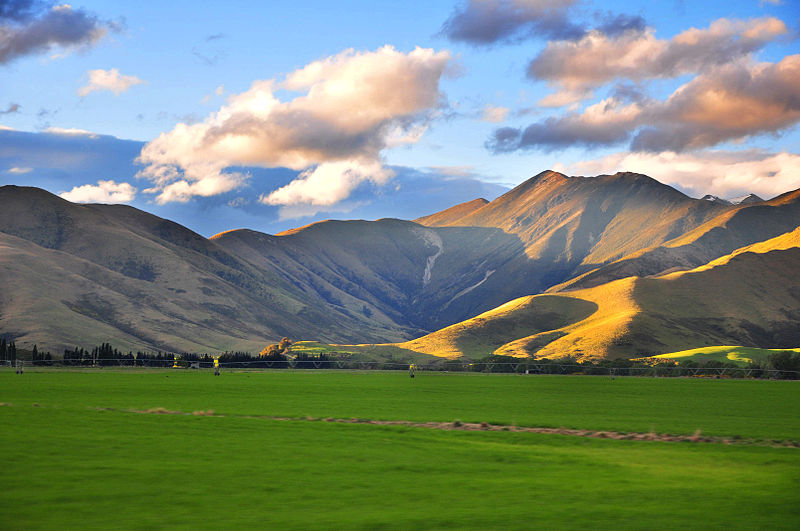
\includegraphics[width=\linewidth]{external/images/nz-landscape.jpg}
\end{image}%
\tcblower
\end{figureptx}%
\footnotetext[1]{\nolinkurl{commons.wikimedia.org/wiki/File:NZ_Landscape_from_the_van.jpg}\label{section-graphics-3-3-1-2}}%
If you have existing images that are vector graphics, then PDF format works best for \LaTeX{} output and SVG format works best for HTML.  The utility \mono{pdf2svg} works well for converting PDF to SVG.  In this case, specify your source as a filename, but leave off the file extension, and the appropriate version will be used for the current output format.%
\par
The image below is provided from a PDF file in \LaTeX{} output, and was converted to an SVG for use with the HTML output.  It has been explicitly scaled to a width of 65\% of the text width.%
\begin{figureptx}{Figure}{Complete graph on \(16\) vertices, from \mono{www.texample.net}}{figure-complete-graph}{}%
\begin{image}{0.175}{0.65}{0.175}{}%
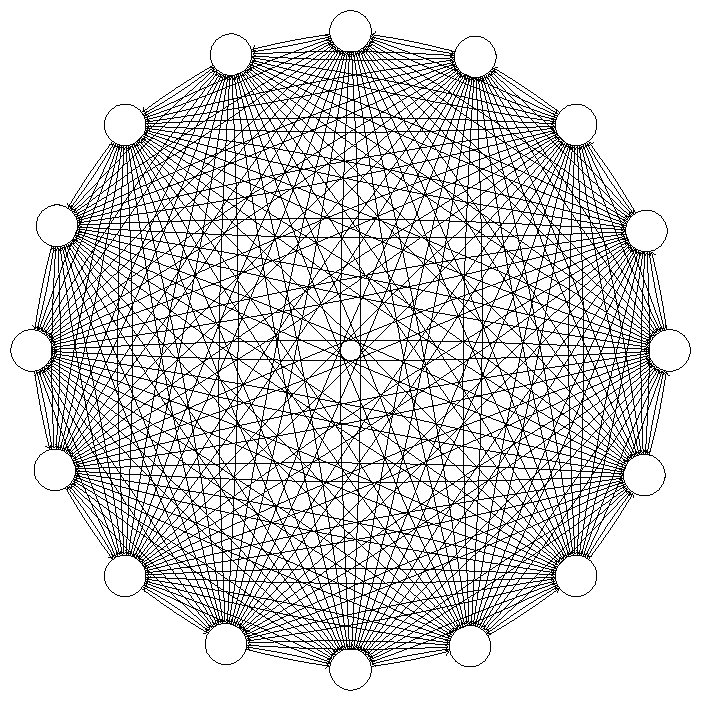
\includegraphics[width=\linewidth]{external/images/complete-graph.pdf}
\end{image}%
\tcblower
\end{figureptx}%
\begin{remark}[Footnote Buried]\label{section-graphics-3-7}%
%
Nested \mono{tcolorbox} (in \LaTeX{} conversion) need special care when footnotes are interior.%
\begin{sidebyside}{2}{0.2}{0.3}{0}%
\begin{sbspanel}{0.25}%
A paragraph interior to a \mono{sidebyside} with a footnote\footnotemark{} buried inside the paragraph.%
\end{sbspanel}%
\begin{sbspanel}{0.25}%
\par
A second paragraph, just to avoid a one-panel warning.%
\end{sbspanel}%
\end{sidebyside}%
\par
The final paragraph of this remark, randomly placed, to test footnotes in \LaTeX{} conversions.%
\end{remark}
\footnotetext[2]{Interior footnote.\label{section-graphics-3-7-3-1-2}}%
% end of subsection: Images from External Sources
%
%
\typeout{************************************************}
\typeout{Subsection 10.2 PreFigure}
\typeout{************************************************}
%
\subsection{PreFigure}\label{prefigure-diagrams}%
\index{PreFigure image}%
\index{image!PreFigure image}%
PreFigure is a standalone project for authoring mathematical diagrams (see \href{https://prefigure.org/}{\nolinkurl{prefigure.org}}).  Its philosophy and approach are much like that of PreTeXt, and PreFigure is tightly integrated into PreTeXt.  One key feature is excellent support for the creation of accessible output formats.%
\par
As of 2024-11-06 development continues for PreFigure itself, and fine-tuning of its integration within PreTeXt.  But it is usable now for projects that want to use it.%
\begin{itemize}[label=\textbullet]
\item{}You can author PreFigure diagrams, and then generate \initialism{SVG}, \initialism{PDF}, and \initialism{PNG} output versions with the \mono{pretext/pretext} script (see the PreTeXt Guide), and expect them to render in \initialism{HTML}, \initialism{PDF}, and \initialism{EPUB} output formats.%
\item{}Look for automatic generation to come to the PreTeXt-CLI sometime very soon.%
\item{}PreFigure has excellent support for annotations within an \initialism{SVG} diagram, supporting their use by screenreaders, for example.  See an example below.%
\item{}Production of tactile versions is now possible, though they are not incorporated explicitly into any of the output formats.  Perhaps they will become available via archive links or as a zip archive.%
\end{itemize}
%
\par
This is a basic PreFigure diagram, in the sense that it does not use all the features of PreFigure or PreTeXt.%
\begin{figureptx}{Figure}{Solution to a differential equation}{prefigure-diagrams-7}{}%
\begin{image}{0.2}{0.6}{0.2}{}%

\includegraphics[width=\linewidth]{generated/prefigure/prefigure-diffeq.pdf}%
\end{image}%
\tcblower
\end{figureptx}%
This next diagram employs some \LaTeX{} macros that are defined in the usual way in \mono{<docinfo>} and are employed to produce the names of some vectors in the labels.  The blue line is colored blue by a global PreFigure declaration, also in \mono{<docinfo>}.%
\begin{image}{0.2}{0.6}{0.2}{}%

\includegraphics[width=\linewidth]{generated/prefigure/prefigure-projection.pdf}%
\end{image}%
The next PreFigure diagram is authored with annotations, arranged in a hierarchy of increasing refinement and detail.  Each identified graphical component will read its annotation and show it on the screen below the diagram.  When a reader clicks on the image, a high-level summary will be read using the author-provided annotation.  The down and up arrow keys enable a reader to explore the diagram in more or less detail while the right and left arrow keys reveal features at the same level of detail.  When the focus is on the graph, pressing "O" will produce a sonification of the graph.%
\begin{image}{0.2}{0.6}{0.2}{}%

\includegraphics[width=\linewidth]{generated/prefigure/prefigure-tangent.pdf}%
\end{image}%
Including annotations enables a new type of interactive diagram within a PreTeXt document offering potential benefits for all readers.  In particular, annotations allow an author to call the reader's attention to specific details in a diagram and how they are related to one another so that the diagram and surrounding text are more tightly integrated.  The annotated diagram below introduces Fibonacci tilings, which are one-dimensional analogs of Penrose tilings, and offers an explanation of their aperiodicity.  Of course, surrounding text would usually provide a richer context for a diagram like this.%
\begin{figureptx}{Figure}{Fibonacci tilings are one-dimensional analogs of Penrose tilings.  The diagram on the left introduces the process of deflation that is used to produce tilings while the diagram on the right explains why they are aperiodic.}{figure-fibonnaci-tiling-annotated}{}%
\begin{sidebyside}{2}{0}{0.15}{0.05}%
\begin{sbspanel}{0.3}[bottom]%
\noindent
\includegraphics[width=\linewidth]{generated/prefigure/prefigure-fibonacci-a.pdf}%
\end{sbspanel}%
\begin{sbspanel}{0.5}[bottom]%
\noindent
\includegraphics[width=\linewidth]{generated/prefigure/prefigure-fibonacci-b.pdf}%
\end{sbspanel}%
\end{sidebyside}%
\tcblower
\end{figureptx}%
For sighted readers, here is an example of a tactile version of one of the above diagrams.  It is generated automatically from the same source as the other version.  Imagine this being ``printed'' with an embosser so that the parts of the diagram, and the braille labels, are raised up from the paper and can be explored with one's fingertips.  This image is a \initialism{PNG} produced specifically for this document.  Typically, a tactile diagram produced by PreFigure will be a \initialism{PDF} ready to be sent to an appropriate embosser.  Notice that PreTeXt adds a caption indicating the diagram's location in the document along the top of the diagram.%
\begin{image}{0.15}{0.7}{0.15}{}%

\includegraphics[width=\linewidth]{external/tactile/prefigure-diffeq.png}
\end{image}%
% end of subsection: PreFigure
%
%
\typeout{************************************************}
\typeout{Subsection 10.3 \LaTeX{} images}
\typeout{************************************************}
%
\subsection{\LaTeX{} images}\label{section-graphics-5}%
\index{\LaTeX{} image}%
\index{image!\LaTeX{} image}%
There are several graphics engine packages that a \LaTeX{} document can employ. Code from these packages renders diagrams automatically as part of normal processing of \LaTeX{} files.  For HTML output the \mono{pretext} script produces SVG versions of the pictures.  The script can also produce standalone \TeX{} source files, PDFs, PNGs, and EPSs. The packages should be loaded in \mono{docinfo/latex-image-preamble}, which is also where global package settings should be made. If any ampersands occur in your \LaTeX{} code you should use the \mono{\textbackslash{}amp} macro pre-defined by PreTeXt. These first examples are from the \href{http://www.texample.net/tikz/examples/}{TeXample.net}\footnote{\nolinkurl{www.texample.net/tikz/examples/}\label{section-graphics-5-4-10}} site.  Note that any \LaTeX{} macros used in the rest of your document may be employed in the \LaTeX{}-standalone or Asymptote diagrams (with this feature coming to Sage graphics next?).%
\begin{figureptx}{Figure}{TikZ Electronics Diagram}{figure-tikz-electronics}{}%
\begin{image}{0}{1}{0}{}%
\resizebox{\linewidth}{!}{%
\tikzset{%
  block/.style    = {draw, thick, rectangle, minimum height = 3em,
    minimum width = 3em},
  sum/.style      = {draw, circle, node distance = 2cm}, % Adder
  input/.style    = {coordinate}, % Input
  output/.style   = {coordinate} % Output
}
% Defining string as labels of certain blocks.
\newcommand{\suma}{\Large$+$}
\newcommand{\inte}{$\displaystyle \int$}
\newcommand{\derv}{\huge$\frac{d}{dt}$}

\begin{tikzpicture}[auto, thick, node distance=2cm, >=triangle 45]
\draw
    % Drawing the blocks of first filter :
    node at (0,0)[right=-3mm]{\Large \textbullet}
    node [input, name=input1] {}
    node [sum, right of=input1] (suma1) {\suma}
    node [block, right of=suma1] (inte1) {\inte}
         node at (6.8,0)[block] (Q1) {\Large $Q_1$}
         node [block, below of=inte1] (ret1) {\Large$T_1$};
    % Joining blocks.
    % Commands \draw with options like [->] must be written individually
    \draw[->](input1) -- node {$X(Z)$}(suma1);
    \draw[->](suma1) -- node {} (inte1);
    \draw[->](inte1) -- node {} (Q1);
    \draw[->](ret1) -| node[near end]{} (suma1);
    % Adder
\draw
    node at (5.4,-4) [sum, name=suma2] {\suma}
        % Second stage of filter
    node at  (1,-6) [sum, name=suma3] {\suma}
    node [block, right of=suma3] (inte2) {\inte}
    node [sum, right of=inte2] (suma4) {\suma}
    node [block, right of=suma4] (inte3) {\inte}
    node [block, right of=inte3] (Q2) {\Large$Q_2$}
    node at (9,-8) [block, name=ret2] {\Large$T_2$}
;
    % Joining the blocks of second filter
    \draw[->] (suma3) -- node {} (inte2);
    \draw[->] (inte2) -- node {} (suma4);
    \draw[->] (suma4) -- node {} (inte3);
    \draw[->] (inte3) -- node {} (Q2);
    \draw[->] (ret2) -| (suma3);
    \draw[->] (ret2) -| (suma4);
         % Third stage of filter:
    % Defining nodes:
\draw
    node at (11.5, 0) [sum, name=suma5]{\suma}
    node [output, right of=suma5]{}
    node [block, below of=suma5] (deriv1){\derv}
    node [output, right of=suma5] (sal2){}
;
    % Joining the blocks:
    \draw[->] (suma2) -| node {}(suma3);
    \draw[->] (Q1) -- (8,0) |- node {}(ret1);
    \draw[->] (8,0) |- (suma2);
    \draw[->] (5.4,0) -- (suma2);
    \draw[->] (Q1) -- node {}(suma5);
    \draw[->] (deriv1) -- node {}(suma5);
    \draw[->] (Q2) -| node {}(deriv1);
        \draw[<->] (ret2) -| node {}(deriv1);
        \draw[->] (suma5) -- node {$Y(Z)$}(sal2);
        % Drawing nodes with \textbullet
\draw
    node at (8,0) {\textbullet}
    node at (8,-2){\textbullet}
    node at (5.4,0){\textbullet}
        node at (5,-8){\textbullet}
        node at (11.5,-6){\textbullet}
        ;
    % Boxing and labelling noise shapers
    \draw [color=gray,thick](-0.5,-3) rectangle (9,1);
    \node at (-0.5,1) [above=5mm, right=0mm] {\textsc{first-order noise shaper}};
    \draw [color=gray,thick](-0.5,-9) rectangle (12.5,-5);
    \node at (-0.5,-9) [below=5mm, right=0mm] {\textsc{second-order noise shaper}};
\end{tikzpicture}%
}%
\end{image}%
\tcblower
\end{figureptx}%
The next example began life in \href{http://www.frontiernet.net/\~eugene.ressler/}{Sketch}\footnote{\nolinkurl{www.frontiernet.net/\~eugene.ressler/}\label{section-graphics-5-6-2}}, which will output TikZ code (though the code has been edited by hand for readability).%
\begin{figureptx}{Figure}{TikZ Cone Drawing}{figure-tikz-cone3D}{}%
\begin{image}{0.15}{0.7}{0.15}{}%
\resizebox{\linewidth}{!}{%
\begin{tikzpicture}[join=round]
\tikzstyle{conefill} = [fill=blue!20,fill opacity=0.8]
\tikzstyle{ann} = [fill=white,font=\footnotesize,inner sep=1pt]
\tikzstyle{ghostfill} = [fill=white]
     \tikzstyle{ghostdraw} = [draw=black!50]
\filldraw[conefill](-.775,1.922)--(-1.162,.283)--(-.274,.5)
                    --(-.183,2.067)--cycle;
\filldraw[conefill](-.183,2.067)--(-.274,.5)--(.775,.424)
                    --(.516,2.016)--cycle;
\filldraw[conefill](.516,2.016)--(.775,.424)--(1.369,.1)
                    --(.913,1.8)--cycle;
\filldraw[conefill](-.913,1.667)--(-1.369,-.1)--(-1.162,.283)
                    --(-.775,1.922)--cycle;
\draw(1.461,.107)--(1.734,.127);
\draw[arrows=<->](1.643,1.853)--(1.643,.12);
\filldraw[conefill](.913,1.8)--(1.369,.1)--(1.162,-.283)
                    --(.775,1.545)--cycle;
\draw[arrows=->,line width=.4pt](.274,-.5)--(0,0)--(0,2.86);
\draw[arrows=-,line width=.4pt](0,0)--(-1.369,-.1);
\draw[arrows=->,line width=.4pt](-1.369,-.1)--(-2.1,-.153);
\filldraw[conefill](-.516,1.45)--(-.775,-.424)--(-1.369,-.1)
                    --(-.913,1.667)--cycle;
\draw(-1.369,.073)--(-1.369,2.76);
\draw(1.004,1.807)--(1.734,1.86);
\filldraw[conefill](.775,1.545)--(1.162,-.283)--(.274,-.5)
                    --(.183,1.4)--cycle;
\draw[arrows=<->](0,2.34)--(-.913,2.273);
\draw(-.913,1.84)--(-.913,2.447);
\draw[arrows=<->](0,2.687)--(-1.369,2.587);
\filldraw[conefill](.183,1.4)--(.274,-.5)--(-.775,-.424)
                    --(-.516,1.45)--cycle;
\draw[arrows=<-,line width=.4pt](.42,-.767)--(.274,-.5);
\node[ann] at (-.456,2.307) {$r_0$};
\node[ann] at (-.685,2.637) {$r_1$};
\node[ann] at (1.643,.987) {$h$};
\path (.42,-.767) node[below] {$x$}
    (0,2.86) node[above] {$y$}
    (-2.1,-.153) node[left] {$z$};
% Second version of the cone
\begin{scope}[xshift=3.5cm]
\filldraw[ghostdraw,ghostfill](-.775,1.922)--(-1.162,.283)--(-.274,.5)
                               --(-.183,2.067)--cycle;
\filldraw[ghostdraw,ghostfill](-.183,2.067)--(-.274,.5)--(.775,.424)
                               --(.516,2.016)--cycle;
\filldraw[ghostdraw,ghostfill](.516,2.016)--(.775,.424)--(1.369,.1)
                               --(.913,1.8)--cycle;
\filldraw[ghostdraw,ghostfill](-.913,1.667)--(-1.369,-.1)--(-1.162,.283)
                               --(-.775,1.922)--cycle;
\filldraw[ghostdraw,ghostfill](.913,1.8)--(1.369,.1)--(1.162,-.283)
                               --(.775,1.545)--cycle;
\filldraw[ghostdraw,ghostfill](-.516,1.45)--(-.775,-.424)--(-1.369,-.1)
                               --(-.913,1.667)--cycle;
\filldraw[ghostdraw,ghostfill](.775,1.545)--(1.162,-.283)--(.274,-.5)
                               --(.183,1.4)--cycle;
\filldraw[fill=red,fill opacity=0.5](-.516,1.45)--(-.775,-.424)--(.274,-.5)
                                     --(.183,1.4)--cycle;
\fill(-.775,-.424) circle (2pt);
\fill(.274,-.5) circle (2pt);
\fill(-.516,1.45) circle (2pt);
\fill(.183,1.4) circle (2pt);
\path[font=\footnotesize]
        (.913,1.8) node[right] {$i\hbox{$=$}0$}
        (1.369,.1) node[right] {$i\hbox{$=$}1$};
\path[font=\footnotesize]
        (-.645,.513) node[left] {$j$}
        (.228,.45) node[right] {$j\hbox{$+$}1$};
\draw (-.209,.482)+(-60:.25) [yscale=1.3,->] arc(-60:240:.25);
\fill[black,font=\footnotesize]
                (-.516,1.45) node [above] {$P_{00}$}
                (-.775,-.424) node [below] {$P_{10}$}
                (.183,1.4) node [above] {$P_{01}$}
                (.274,-.5) node [below] {$P_{11}$};
\end{scope}
\end{tikzpicture}%
}%
\end{image}%
\tcblower
\end{figureptx}%
The pgfplots package was included in \mono{docinfo/latex-image-preamble}. Here, it is used. Also, here we demonstrate using \mono{\textbackslash{}amp} where you would normally use an ampersand in \LaTeX{}. There are known issues with \mono{xelatex} processing any gradient shading in \mono{tikz}. To (successfully) create the gradient shading in the 3D image here, you may need to use \mono{pdflatex} until \LaTeX{} developers resolve this issue.%
\begin{figureptx}{Figure}{Sample pgfplots plot}{figure-pgfplots-demo}{}%
\begin{image}{0}{1}{0}{}%
\resizebox{\linewidth}{!}{%
\begin{tikzpicture}
\matrix{
    \begin{axis}[width = 0.5\linewidth]
        \addplot[
            domain = 0.1:10,
            <->,
            smooth,
            thin,
            color = blue,
        ]{4*ln(x)/ln(10)};
        \addplot[
            only marks,
        ]coordinates{
            (0,2)
            (4,3)
            (2,4)
            (3,4)};
        \addplot[
            variable = \t,
            domain = 0:360,
            samples = 200,
            color = orange,
        ]({3*sin(2*t)}, {2*cos(5*t)});
    \end{axis}
    \amp
    \begin{axis}[axis lines = box, width = 0.5\linewidth]
        \addplot3[
            surf,
            faceted color = blue,
            samples = 15,
            domain = 0:1,
            y domain = -1:1
        ]{x^2 - y^2};
    \end{axis}\\
};
\end{tikzpicture}%
}%
\end{image}%
\tcblower
\end{figureptx}%
A plot might use a graphics language to draw the axes and grid, but the data might be from an experiment and live in an external file that you do not wish to place in your source.  Place such a file in a subdirectory directly below the directory where your master source file resides.  In the example below \mono{data} is the directory and \mono{hodgkin-huxley-data.dat} is the file with the data points.  You \emph{must} place the file in a subdirectory (it cannot reside next to your source file), but that directory may have subdirectories if you have many such files and want to organize them that way.  Then the \mono{--include} command-line argument to the \mono{pretext} script will manage the external files properly as it creates individual image files.%
\par
It is still your responsibility to be sure this directory of external data files follows your \LaTeX{} output to whatever directory you use to convert to a PDF and is in the right location for the relative path given in the XML source.  The discussion above only applies to generating individual image files, such as you would need for the HTML output.%
\begin{figureptx}{Figure}{External data in a pgfplots plot}{figure-pgfplots-data-demo}{}%
\begin{image}{0}{1}{0}{}%
\resizebox{\linewidth}{!}{%
\begin{tikzpicture}
\begin{axis}[
    xmin=0,xmax=100,ymin=-20,ymax=100,
    ytick={-20,0,...,100},
    xlabel={time (ms)},
    ylabel={potential (V)},
]
\addplot[blue] table {external/data/hodgkin-huxley-data.dat};
\end{axis}
\end{tikzpicture}%
}%
\end{image}%
\tcblower
\end{figureptx}%
A Cartesian plot might benefit from having a \mono{<description>} with a \mono{<tabular>} that lays bare the data used to to plot points.%
\begin{figureptx}{Figure}{Full description with tabular}{figure-pgfplots-data-description}{}%
\begin{image}{0.15}{0.7}{0.15}{}%
\resizebox{\linewidth}{!}{%
\begin{tikzpicture}
    \begin{axis}[
            xmin=0,
            xmax=10,
            ymin=-0,ymax=10,
            xlabel={\(x\)},
            ylabel={\(y\)},
        ]
        \addplot[only marks] coordinates {(1,5) (2,3) (3,8) (4,9) (5,5) (6,5) (7,8) (8,2) (9,3)};
    \end{axis}
\end{tikzpicture}%
}%
\end{image}%
\tcblower
\end{figureptx}%
The next image requires three passes with \LaTeX{} to get everything in place.  It is placed here to test that the code in the Pythion script correctly recognizes this requirement.%
\begin{figureptx}{Figure}{A matrix with colored entries}{section-graphics-5-16}{}%
\begin{image}{0.25}{0.5}{0.25}{}%
\resizebox{\linewidth}{!}{%
    \begin{tikzpicture}
    \node{
        $\begin{bNiceArray}{ccc|cc}[
        code-before={\cellcolor{green!72}{1-1,2-2,3-3}\cellcolor{teal!72}{1-2,2-3,3-4}\cellcolor{yellow!72}{1-3,2-4,3-5}}
        ]
        3 \amp 4 \amp 0 \amp 1 \amp 4 \\
        -2 \amp 3 \amp 1 \amp -2 \amp 3 \\
        0 \amp 2 \amp 1 \amp 0 \amp 2
        \end{bNiceArray}$
    };
\end{tikzpicture}%
}%
\end{image}%
\tcblower
\end{figureptx}%
PSTricks is a \LaTeX{} package for drawing diagrams and pictures, dating back to the days before \initialism{PDF}, when PostScript (\initialism{PS}) was king.  Given its history, it does not seem to work easily with the \mono{pdflatex} engine.  But it will work easily with the \mono{xelatex} engine.  We try to keep this present sample document workable with both engines, so we have presented an example of the use of PSTricks in the \mono{xelatex}-exclusive sample document where we test obscure fonts and characters.  So your best bet is to look there.\index{PSTricks}%
\par
There are suggestions online that%
\begin{codedisplay}
\usepackage[pdf]{pstricks}
\end{codedisplay}
along with%
\begin{codedisplay}
pdflatex --shell-escape *.tex
\end{codedisplay}
is workable.  We could not make it happen, and a ``shell escape'' can be a dangerous security hole.  That said, updates to this approach are welcome.%
% end of subsection: \LaTeX{} images
%
%
\typeout{************************************************}
\typeout{Subsection 10.4 Asymptote, 2D}
\typeout{************************************************}
%
\subsection{Asymptote, 2D}\label{section-graphics-6}%
The Asymptote\index{asymptote graphics language} graphics language may be placed in your source to draw graphs, diagrams or pictures.  Rules for formatting code are identical to those for Sage code.  For more on Asymptote see \href{http://asymptote.sourceforge.net/}{\nolinkurl{asymptote.sourceforge.net}}.%
\par
This is a simple physics diagram about levers, taken from the Asymptote documentation.  In the HTML version of this article, the images are SVG's and so should scale nicely when you zoom in on the page.%
\begin{figureptx}{Figure}{Asymptote Lever Demonstration}{figure-asymptote-levers}{}%
\begin{image}{0}{1}{0}{}%
\href{https://pretextbook.org/examples/sample-article/html/generated/asymptote/asymptote-lever.html}{
\includegraphics[width=\linewidth]{generated/asymptote/asymptote-lever.pdf}}
\end{image}%
\tcblower
\end{figureptx}%
And a colorful contour plot with logarithmic scale.  Again, from the Asymptote documentation.  This SVG image employs two additional PNG images for the two parts where the color varies continuously.%
\begin{figureptx}{Figure}{Asymptote Contour Plot}{figure-asymptote-contour-plot}{}%
\begin{image}{0}{1}{0}{}%
\href{https://pretextbook.org/examples/sample-article/html/generated/asymptote/asymptote-contour.html}{
\includegraphics[width=\linewidth]{generated/asymptote/asymptote-contour.pdf}}
\end{image}%
\tcblower
\end{figureptx}%
Here is the lever diagram again, but now we have added an integral to one of the legends, \emph{using a \LaTeX{} macro of our own,} which is idential to one we used in the early part of this article.  The point is, we only needed to define the macro once for the entire document, and it is available as we make Asymptote diagrams.  This device can be used to maintain flexibility and consistency in your choice of notation.%
\begin{figureptx}{Figure}{Aymptote Lever, plus Integral}{figure-asymptote-latex-macro}{}%
\begin{image}{0.1}{0.8}{0.1}{}%
\href{https://pretextbook.org/examples/sample-article/html/generated/asymptote/asymptote-lever-integral.html}{
\includegraphics[width=\linewidth]{generated/asymptote/asymptote-lever-integral.pdf}}
\end{image}%
\tcblower
\end{figureptx}%
% end of subsection: Asymptote, 2D
%
%
\typeout{************************************************}
\typeout{Subsection 10.5 Asymptote, 3D via WebGL}
\typeout{************************************************}
%
\subsection{Asymptote, 3D via WebGL}\label{graphics-asymptote-webgl}%
Asymptote can create an \initialism{HTML} file that is an interactive version of a 3D shape.  At this writing (2020-05-18) support via the \mono{pretext} script is evolving.  Plus, you will need newer versions of Asymptote and the \mono{dvisvgm} utility to duplicate all of the results being displayed here in this testing document.  The other distinction is that the author needs to provide the aspect ratio of the figure, and this should be placed on the \mono{<asymptote>} element (not on the \mono{<image>} element).  \hyperref[figure-asymptote-workcone]{Figure~{\xreffont\ref{figure-asymptote-workcone}}} is from the \href{http://asymptote.sourceforge.net/gallery/3Dwebgl/}{Asymptote Gallery}\footnote{\nolinkurl{asymptote.sourceforge.net/gallery/3Dwebgl/}\label{graphics-asymptote-webgl-2-8}}.%
\begin{figureptx}{Figure}{Work Cone (Asymptote Interactive 3D Image)}{figure-asymptote-workcone}{}%
\begin{image}{0.25}{0.5}{0.25}{}%
\href{https://pretextbook.org/examples/sample-article/html/generated/asymptote/asymptote-workcone.html}{
\includegraphics[width=\linewidth]{generated/asymptote/asymptote-workcone.pdf}}
\end{image}%
\tcblower
\end{figureptx}%
These 3D images in HTML output are rotable with a pointing device (mouse, trackpad) with a click-and-drag.  A finger should suffice on touch-sensitive devices (phones, tablets).  Zooming in and out can be accomplished with a mouse wheel, or by pinching.  As a contribution to the accessibility of PreTeXt HTML output, keyboard controls will also allow for exploration of these images.  (Make sure the image has focus when you attempt to use these.)%
\begin{tableptx}{Table}{\textbf{3D Image Keyboard Controls}}{graphics-asymptote-webgl-5}{}%
\centering%
{\tabularfont%
\begin{tabular}{ll}
Key&Action\tabularnewline\hrulemedium
\kbd{x}&Rotate around \(x\)-axis\tabularnewline[0pt]
\kbd{y}&Rotate around \(y\)-axis\tabularnewline[0pt]
\kbd{z}&Rotate around \(z\)-axis\tabularnewline[0pt]
\kbd{+}&Enlarge image\tabularnewline[0pt]
\kbd{-}&Shrink image\tabularnewline[0pt]
\kbd{h}&Return to home position
\end{tabular}
}%
\end{tableptx}%
And finally, an example of a 3-D graph (from the Asymptote documentation again).  This WebGL image is a beautiful example of a Riemann surface.  As you rotate the image, notice how the reflection of the light source varies, along with the brightness of various regions of the surface.  This example is accomplished with just 10 lines of Asymptote code.%
\begin{figureptx}{Figure}{Asymptote 3-D Surface}{figure-asymptote-surface}{}%
\begin{image}{0.3}{0.4}{0.3}{}%
\href{https://pretextbook.org/examples/sample-article/html/generated/asymptote/asymptote-surface.html}{
\includegraphics[width=\linewidth]{generated/asymptote/asymptote-surface.pdf}}
\end{image}%
\tcblower
\end{figureptx}%
% end of subsection: Asymptote, 3D via WebGL
%
%
\typeout{************************************************}
\typeout{Subsection 10.6 Mermaid Diagrams}
\typeout{************************************************}
%
\subsection{Mermaid Diagrams}\label{graphics-mermaid}%
\index{Mermaid diagrams}%
\href{https://mermaid.js.org/}{Mermaid}\footnote{\nolinkurl{mermaid.js.org}\label{graphics-mermaid-3-2}} is a Markdown-inspired tool for authoring various kinds of diagrams. Below, three of the available diagram types are demonstrated. For a full listing of diagram types, see the \href{https://mermaid.js.org/intro/\#diagram-types}{Mermaid Documentation}\footnote{\nolinkurl{mermaid.js.org/intro/\#diagram-types}\label{graphics-mermaid-3-4}}. The \href{https://mermaid.live/}{Mermaid live editor}\footnote{\nolinkurl{mermaid.live}\label{graphics-mermaid-3-6}}is a great tool for testing the syntax of your mermaid diagrams.%
\par
In PreTeXt, you can specify a Mermaid theme via \mono{@common\textbackslash{}slash\{\}mermaid\textbackslash{}slash\{\}@theme}%
\begin{figureptx}{Figure}{Mermaid Git Diagram}{figure-mermaid-git}{}%
\begin{image}{0}{1}{0}{}%

\includegraphics[width=\linewidth]{generated/mermaid/mermaid-git-image-color.png}
\end{image}%
\tcblower
\end{figureptx}%
\begin{figureptx}{Figure}{Mermaid Class Diagram}{figure-mermaid-class}{}%
\begin{image}{0}{1}{0}{}%

\includegraphics[width=\linewidth]{generated/mermaid/mermaid-class-image-color.png}
\end{image}%
\tcblower
\end{figureptx}%
\begin{figureptx}{Figure}{Mermaid Seuqnece Diagram}{figure-mermaid-sequence}{}%
\begin{image}{0}{1}{0}{}%

\includegraphics[width=\linewidth]{generated/mermaid/mermaid-sequence-image-color.png}
\end{image}%
\tcblower
\end{figureptx}%
% end of subsection: Mermaid Diagrams
%
%
\typeout{************************************************}
\typeout{Subsection 10.7 Sage Plots}
\typeout{************************************************}
%
\subsection{Sage Plots}\label{section-graphics-9}%
\index{Sage plots}%
Any of the numerous capabilities of Sage may be used to produce any graphics object, be it the simple graph of a single-variable function or some realization of a more complicated object.  All of the usual rules about formatting Sage code (esp. indentation) apply, along with one more caveat.  The last line of your Sage code \alert{must} return a Sage \mono{Graphics} object (or 3D plot).  The \mono{pretext} script will isolate this last line, use it as the RHS of an assignment statement, and the Sage \mono{.save()} method will be called to generate the image, which is either a Portable Document Format (PDF) file amenable to \LaTeX{} output, or a Scalable Vector Graphics (SVG) file amenable to HTML output.  For visualizations of 3D plots, Sage will only produce Portable Network Graphics (PNG) files, which can be included in HTML pages or \LaTeX{} output.  For complete documentation, see the PreTeXt Guide as this subsection is not comprehensive.%
\begin{figureptx}{Figure}{A Sage standard parabola, on \([-2,4]\)}{figure-sage-parabola}{}%
\begin{image}{0.25}{0.5}{0.25}{}%

\includegraphics[width=\linewidth]{generated/sageplot/sageplot-parabola.pdf}%
\end{image}%
\tcblower
\end{figureptx}%
Pay careful attention to the requirement that the last line of your code be a graphics object.  In particular, while \mono{show()} might appear to do the right thing, it evaluates to Python's \mono{None} object and that is just what you will get.  The code for Figure~\hyperref[figure-sage-double-plot]{{\xreffont\ref{figure-sage-double-plot}}} illustrates creating two graphics objects and combining them into an expression on the last line that evaluates to a graphics object.%
\begin{figureptx}{Figure}{Two Sage plots on one set of axes}{figure-sage-double-plot}{}%
\begin{image}{0.275}{0.45}{0.275}{}%

\includegraphics[width=\linewidth]{generated/sageplot/sageplot-updown.pdf}%
\end{image}%
\tcblower
\end{figureptx}%
Sage code comprised of just a single line was once mishandled, leading to \emph{no ouput}.  From Jean-Sébastien Turcotte we have the example that revealed the problem.%
\begin{figureptx}{Figure}{Les vecteurs \(\vec{u}\) et \(\vec{v}\)}{figure-sage-exosagevec1}{}%
\begin{image}{0.375}{0.25}{0.375}{}%

\includegraphics[width=\linewidth]{generated/sageplot/sageplot-exosagevec1.pdf}%
\end{image}%
\tcblower
\end{figureptx}%
The following examples are from the \href{http://www.sagemath.org/tour-graphics.html}{Sage Tour}\footnote{\nolinkurl{www.sagemath.org/tour-graphics.html}\label{section-graphics-9-9-2}}.  We package them into a \mono{sidebyside} layout element, see \hyperref[section-side-by-side]{Section~{\xreffont\ref{section-side-by-side}}}.%
\begin{sidebyside}{2}{0.05}{0.05}{0.1}%
\begin{sbspanel}{0.4}%
\begin{panelfigureptx}{Figure}{A Sage multigraph of a sentence}{figure-sage-multigraph}{}%
\noindent
\includegraphics[width=\linewidth]{generated/sageplot/sageplot-sentence-multigraph.pdf}%
\tcblower
\end{panelfigureptx}%
\end{sbspanel}%
\begin{sbspanel}{0.4}%
\begin{panelfigureptx}{Figure}{Sage polynomial approximations of \(f(x)=1/(1+25x^2)\)}{figure-sage-polynomial-approximation}{}%
\noindent
\includegraphics[width=\linewidth]{generated/sageplot/sageplot-polynomial-approximation.pdf}%
\tcblower
\end{panelfigureptx}%
\end{sbspanel}%
\end{sidebyside}%
\par
From the Sage documentation, with slight modifications, credited to Douglas Summers-Stay.  A plot of the implicity defined surface%
\begin{equation*}
2 = \cos(x + ty) + \cos(x - ty) + \cos(y + tz) + \cos(y - tz) + \cos(z - tx) + \cos(z + tx)
\end{equation*}
in rectangular \(xyz\) coordinates, with \(t\) equal to the golden ratio.  If you set \mono{plot\_points=100} in the Sage code, you will get a very smooth rendering, but also a quite large \initialism{HTML} file.  We have used \mono{plot\_points=50} to reduce the file size by a factor of four.  Note the need for a value of \mono{3d} for the \mono{@variant} attribute, and an explicit aspect ratio with \mono{@aspect}.  Arrow keys, a mouse scroll wheel, plus grabbing with a left or a right mouse button, can be used to manipulate the image.%
\begin{figureptx}{Figure}{A Sage implicitly defined 3D surface}{figure-sage-implicit-surface}{}%
\begin{image}{0.15}{0.8}{0.05}{}%

\includegraphics[width=\linewidth]{generated/sageplot/sageplot-implicit-surface.png}%
\end{image}%
\tcblower
\end{figureptx}%
% end of subsection: Sage Plots
%
%
\typeout{************************************************}
\typeout{Subsection 10.8 Inkscape Images}
\typeout{************************************************}
%
\subsection{Inkscape Images}\label{section-graphics-10}%
\href{https://inkscape.org/}{Inkscape}\footnote{\nolinkurl{inkscape.org}\label{section-graphics-10-2-2}} is a great tool for creating images.  It ticks all the boxes: open source, mature, cross-platform, standards-compliant.  Read much more about it in The PreTeXt Guide.  In \initialism{HTML} output the two images below are both in \initialism{SVG} format.  The first is ``pure'' SVG, while the second has embedded information that makes it easier to edit in Inkscape.  You could view the source for this page in the \initialism{HTML} version, deduce the filename of the second image, download it, and manipulate it profitably with Inkscape.  Both files are quite small, but the first is half the size of the second.  In \initialism{PDF} the two images come from files that are identical, so nothing is being tested.  The \initialism{PDF} version is smaller still.%
\begin{figureptx}{Figure}{Inkscape Stars, Plain SVG (left), Inkscape SVG (right), from Bethany Llewellyn}{section-graphics-10-3}{}%
\begin{sidebyside}{2}{0.125}{0.125}{0.25}%
\begin{sbspanel}{0.25}%
\noindent
\includegraphics[width=\linewidth]{external/images/inkscape-stars-plain.pdf}
\end{sbspanel}%
\begin{sbspanel}{0.25}%
\noindent
\includegraphics[width=\linewidth]{external/images/inkscape-stars-native.pdf}
\end{sbspanel}%
\end{sidebyside}%
\tcblower
\end{figureptx}%
% end of subsection: Inkscape Images
%
%
\typeout{************************************************}
\typeout{Subsection 10.9 Copies of Images}
\typeout{************************************************}
%
\subsection{Copies of Images}\label{section-graphics-11}%
Sometimes you want to use the same image more than once.  Here we just point to a \initialism{PNG} file that we repeat often throughout this sample.%
\begin{figureptx}{Figure}{Copy of raster image, in a figure, so now numbered and captioned}{figure-raster-image-copy}{}%
\begin{image}{0.35}{0.3}{0.35}{}%

\includegraphics[width=\linewidth]{external/images/cross-square.png}
\end{image}%
\tcblower
\end{figureptx}%
For images described by code, such as TikZ code in a \mono{<latex-image>} element, this is a bit subtler.  See the PreTeXt Guide for a complete description.  We also demonstrate this with the sample book, since it is all set up with the \mono{xinclude} mechanism.  See the two plots of the 8-th roots of unity in the complex numbers section of the chapter on cyclic groups.%
% end of subsection: Copies of Images
%
%
\typeout{************************************************}
\typeout{Subsection 10.10 Caption Testing}
\typeout{************************************************}
%
\subsection{Caption Testing}\label{section-graphics-12}%
A caption could be as substantial as a paragraph, here we test out one such example.%
\begin{figureptx}{Figure}{A caption can be a whole paragraph with lots of technical details, and maybe a hyperlink to something external, such as \href{https://pretextbook.org}{\nolinkurl{pretextbook.org}} or \href{https://pretextbook.org}{PreTeXt}\protect\footnotemark{}.  There could be some inline mathematics, such as \(x^2 + y^2 = c^2\).  Would a knowl open here?  Recursively?  Let's see: \hyperref[figure-long-caption]{{\xreffont\ref{figure-long-caption}}}.  Display mathematics, side-by-sides, theorems, and lots of other things should be banned.  Footnotes sound like a bad idea.  Strange characters should be fine: \textsection{}.}{figure-long-caption}{}%
\begin{image}{0.4}{0.2}{0.4}{}%

\includegraphics[width=\linewidth]{external/images/cross-square.png}
\end{image}%
\tcblower
\end{figureptx}%
\footnotetext[11]{\nolinkurl{pretextbook.org}\label{figure-long-caption-1-3}}%
% end of subsection: Caption Testing
%
%
\typeout{************************************************}
\typeout{Subsection 10.11 Captionless Images}
\typeout{************************************************}
%
\subsection{Captionless Images}\label{captionless-images}%
We strongly suggest placing images within a \mono{<figure>}, as we have done above, so that you can reference them, and use the (required) \mono{<caption>} to explain what they are.  However there are places, such as a \mono{<preface>}, where numbered items are not permitted.  So you might want a solo image there.  Or maybe graphics are an illustration of sorts, and a numbered figure feels like overkill.  Or it is part of an \mono{<exercise>} or \mono{<proof>} of a \mono{<theorem>}. But notice that you cannot then use this image as the target of a cross-reference, so you may need to refer to some enclosing container.%
\par
The image can be scaled by specifying the \mono{@width} as a percentage, including the percent-sign (\%).  The height is scaled to preserve the aspect ratio.  There is no facility to change the height, it is your responsibility to manage the aspect ratio independently.  The \mono{@margins} can be given as a pair of percentages, separated by a space.  The \mono{@width} defaults to 100\%, while \mono{@margins} defaults to the value \mono{auto}, which will center the image.  Missing values are computed sensibly, and there is robust error-checking.  The layout control here is a subset of what is available for the more elaborate \mono{<sidebyside>} element, see \hyperref[section-side-by-side]{Section~{\xreffont\ref{section-side-by-side}}}.%
\par
Two simple examples. The first has width \mono{10\%} and so defaults to being centered, and the second has width \mono{10\%} and left margin of \mono{25\%}.%
\begin{image}{0.45}{0.1}{0.45}{}%

\includegraphics[width=\linewidth]{external/images/cross-square.png}
\end{image}%
A paragraph, just to show where the first stops and the second ends.%
\begin{image}{0.25}{0.1}{0.65}{}%

\includegraphics[width=\linewidth]{external/images/cross-square.png}
\end{image}%
You might wish to place a single image flush-left, or flush-right.  You can specify the \mono{margins} attribute as a pair of percentages for different left and right margins.  The following are laid out with two margins, with a 0\% left margin and right margin (respectively).%
\begin{image}{0}{0.1}{0.9}{}%

\includegraphics[width=\linewidth]{external/images/cross-square.png}
\end{image}%
\begin{image}{0.9}{0.1}{0}{}%

\includegraphics[width=\linewidth]{external/images/cross-square.png}
\end{image}%
We place two images right above one another, to test spacing of consecutive images (provided they stay on the same page!).%
\begin{image}{0.1}{0.1}{0.8}{}%

\includegraphics[width=\linewidth]{external/images/cross-square.png}
\end{image}%
\begin{image}{0.1}{0.1}{0.8}{}%

\includegraphics[width=\linewidth]{external/images/cross-square.png}
\end{image}%
\subsubsection*{Testing (2019-06-02).}\label{captionless-images-14}%
All the images above are specified by filenames.  We need to test how various options behave when incorporated into the (new) implementation for images, being introduced with solo images.%
\par
A \mono{tikz} image recycled from above, now 40\% width, with 40\% left margin, 20\% right margin.%
\begin{image}{0.4}{0.4}{0.2}{}%
\resizebox{\linewidth}{!}{%
\begin{tikzpicture}[join=round]
\tikzstyle{conefill} = [fill=blue!20,fill opacity=0.8]
\tikzstyle{ann} = [fill=white,font=\footnotesize,inner sep=1pt]
\tikzstyle{ghostfill} = [fill=white]
     \tikzstyle{ghostdraw} = [draw=black!50]
\filldraw[conefill](-.775,1.922)--(-1.162,.283)--(-.274,.5)
                    --(-.183,2.067)--cycle;
\filldraw[conefill](-.183,2.067)--(-.274,.5)--(.775,.424)
                    --(.516,2.016)--cycle;
\filldraw[conefill](.516,2.016)--(.775,.424)--(1.369,.1)
                    --(.913,1.8)--cycle;
\filldraw[conefill](-.913,1.667)--(-1.369,-.1)--(-1.162,.283)
                    --(-.775,1.922)--cycle;
\draw(1.461,.107)--(1.734,.127);
\draw[arrows=<->](1.643,1.853)--(1.643,.12);
\filldraw[conefill](.913,1.8)--(1.369,.1)--(1.162,-.283)
                    --(.775,1.545)--cycle;
\draw[arrows=->,line width=.4pt](.274,-.5)--(0,0)--(0,2.86);
\draw[arrows=-,line width=.4pt](0,0)--(-1.369,-.1);
\draw[arrows=->,line width=.4pt](-1.369,-.1)--(-2.1,-.153);
\filldraw[conefill](-.516,1.45)--(-.775,-.424)--(-1.369,-.1)
                    --(-.913,1.667)--cycle;
\draw(-1.369,.073)--(-1.369,2.76);
\draw(1.004,1.807)--(1.734,1.86);
\filldraw[conefill](.775,1.545)--(1.162,-.283)--(.274,-.5)
                    --(.183,1.4)--cycle;
\draw[arrows=<->](0,2.34)--(-.913,2.273);
\draw(-.913,1.84)--(-.913,2.447);
\draw[arrows=<->](0,2.687)--(-1.369,2.587);
\filldraw[conefill](.183,1.4)--(.274,-.5)--(-.775,-.424)
                    --(-.516,1.45)--cycle;
\draw[arrows=<-,line width=.4pt](.42,-.767)--(.274,-.5);
\node[ann] at (-.456,2.307) {$r_0$};
\node[ann] at (-.685,2.637) {$r_1$};
\node[ann] at (1.643,.987) {$h$};
\path (.42,-.767) node[below] {$x$}
    (0,2.86) node[above] {$y$}
    (-2.1,-.153) node[left] {$z$};
% Second version of the cone
\begin{scope}[xshift=3.5cm]
\filldraw[ghostdraw,ghostfill](-.775,1.922)--(-1.162,.283)--(-.274,.5)
                               --(-.183,2.067)--cycle;
\filldraw[ghostdraw,ghostfill](-.183,2.067)--(-.274,.5)--(.775,.424)
                               --(.516,2.016)--cycle;
\filldraw[ghostdraw,ghostfill](.516,2.016)--(.775,.424)--(1.369,.1)
                               --(.913,1.8)--cycle;
\filldraw[ghostdraw,ghostfill](-.913,1.667)--(-1.369,-.1)--(-1.162,.283)
                               --(-.775,1.922)--cycle;
\filldraw[ghostdraw,ghostfill](.913,1.8)--(1.369,.1)--(1.162,-.283)
                               --(.775,1.545)--cycle;
\filldraw[ghostdraw,ghostfill](-.516,1.45)--(-.775,-.424)--(-1.369,-.1)
                               --(-.913,1.667)--cycle;
\filldraw[ghostdraw,ghostfill](.775,1.545)--(1.162,-.283)--(.274,-.5)
                               --(.183,1.4)--cycle;
\filldraw[fill=red,fill opacity=0.5](-.516,1.45)--(-.775,-.424)--(.274,-.5)
                                     --(.183,1.4)--cycle;
\fill(-.775,-.424) circle (2pt);
\fill(.274,-.5) circle (2pt);
\fill(-.516,1.45) circle (2pt);
\fill(.183,1.4) circle (2pt);
\path[font=\footnotesize]
        (.913,1.8) node[right] {$i\hbox{$=$}0$}
        (1.369,.1) node[right] {$i\hbox{$=$}1$};
\path[font=\footnotesize]
        (-.645,.513) node[left] {$j$}
        (.228,.45) node[right] {$j\hbox{$+$}1$};
\draw (-.209,.482)+(-60:.25) [yscale=1.3,->] arc(-60:240:.25);
\fill[black,font=\footnotesize]
                (-.516,1.45) node [above] {$P_{00}$}
                (-.775,-.424) node [below] {$P_{10}$}
                (.183,1.4) node [above] {$P_{01}$}
                (.274,-.5) node [below] {$P_{11}$};
\end{scope}
\end{tikzpicture}%
}%
\end{image}%
A \mono{pgfplot} image recycled from above, now 20\% width, with 40\% left margin, 40\% right margin, and no longer legible.%
\begin{image}{0.4}{0.2}{0.4}{}%
\resizebox{\linewidth}{!}{%
\begin{tikzpicture}
\begin{axis}[
    xmin=0,xmax=100,ymin=-20,ymax=100,
    ytick={-20,0,...,100},
    xlabel={time (ms)},
    ylabel={potential (V)},
]
\addplot[blue] table {external/data/hodgkin-huxley-data.dat};
\end{axis}
\end{tikzpicture}%
}%
\end{image}%
An Asymptote image, with zero layout control, so 100\% width.%
\begin{image}{0}{1}{0}{}%
\href{https://pretextbook.org/examples/sample-article/html/generated/asymptote/asymptote-lever-solo.html}{
\includegraphics[width=\linewidth]{generated/asymptote/asymptote-lever-solo.pdf}}
\end{image}%
A Sage example, pushed to the right margin.%
\begin{image}{0.7}{0.3}{0}{}%

\includegraphics[width=\linewidth]{generated/sageplot/sageplot-parabola-solo.pdf}%
\end{image}%
% end of paragraphs
% end of subsection: Captionless Images
%
%
\typeout{************************************************}
\typeout{Subsection 10.12 Technical Details}
\typeout{************************************************}
%
\subsection{Technical Details}\label{section-graphics-14}%
The table below is a summary of how graphics and images are specified, constructed and manipulated.  Additional processing is indicated by reference to the Python script \mono{pretext}.  Images need to be placed relative to the \LaTeX{} file that includes them during compilation, and placed relative to the \initialism{HTML} files which reference\slash{}include them.  Author-provided image files may be placed in any subdirectory, and the \mono{@source} attribute should include the complete relative path with the subdirectory.  Files generated by the \mono{pretext} script will be specified in the output using the relative directory \mono{images}, which can be changed.  There is no reason author-provided files cannot also be placed in this same directory (presuming no duplicate names). [This table is presently more readable in HTML, the PDF version will improve.]%
\begin{center}%
{\tabularfont%
\begin{tabular}{lllll}\hrulemedium
Element&Specification&\LaTeX{}\slash{}Print&HTML&Notes\tabularnewline\hrulemedium
\mono{image/@source}&full relative path, w\slash{} extension&directly included&directly included&author-provided \initialism{PNG}, \initialism{JPEG}\tabularnewline\hrulethin
\mono{image/@source}&full relative path, w\slash{}o extension&presumes \initialism{PDF}&presumes \initialism{SVG}&author-provided\tabularnewline\hrulethin
\mono{image/latex-image-code}&\LaTeX{}-compatible source&directly included&\initialism{SVG} via \mono{pretext}&e.g.\@ tikz, pgfplots, xypic\tabularnewline\hrulethin
\mono{image/sageplot}&Sage code&\initialism{PDF} via \mono{pretext}&\initialism{SVG} via \mono{pretext}&\initialism{PNG} for 3-D\tabularnewline\hrulethin
\mono{image/asymptote}&Asymptote code&\initialism{PDF} via \mono{pretext}&\initialism{SVG} via \mono{pretext}&\tabularnewline\hrulethin
\end{tabular}
}%
\end{center}%
In the early stages of a writing project, it may be best not to track provisional image files built with \mono{pretext} under version control, and just regenerate them periodically (see the \mono{-r} option for \mono{pretext}).  As a project matures, then it makes sense to put stable files under version control for collaborators and others.  In every case, managing graphics files (and other aspects of production), is much more pleasurable with a script (shell, Makefile, etc.)%
% end of subsection: Technical Details
%
%
\typeout{************************************************}
\typeout{Subsection 10.13 Accessibility}
\typeout{************************************************}
%
\subsection{Accessibility}\label{section-graphics-15}%
An \mono{<image>} should either have a non-empty \mono{<description>}, a non-empty \mono{<shortdescription>}, or set \mono{@decorative} to the value \mono{yes}. Some of the following images comply, and some do not.  There's not really anything to see here visually, this is testing notifications made elsewhere.%
\begin{sidebyside}{4}{0.025}{0.025}{0.05}%
\begin{sbspanel}{0.2}%
No description, no shortdescription, no \mono{@decorative} set to \mono{yes}%
\end{sbspanel}%
\begin{sbspanel}{0.2}%
\noindent
\includegraphics[width=\linewidth]{external/images/cross-square.png}
\end{sbspanel}%
\begin{sbspanel}{0.2}%
No description, no shortdescription, \mono{@decorative} set to \mono{yes}%
\end{sbspanel}%
\begin{sbspanel}{0.2}%
\noindent
\includegraphics[width=\linewidth]{external/images/cross-square.png}
\end{sbspanel}%
\end{sidebyside}%
\begin{sidebyside}{4}{0.025}{0.025}{0.05}%
\begin{sbspanel}{0.2}%
No description, empty shortdescription, no \mono{@decorative} set to \mono{yes}%
\end{sbspanel}%
\begin{sbspanel}{0.2}%
\noindent
\includegraphics[width=\linewidth]{external/images/cross-square.png}
\end{sbspanel}%
\begin{sbspanel}{0.2}%
No description, empty shortdescription, \mono{@decorative} set to \mono{yes}%
\end{sbspanel}%
\begin{sbspanel}{0.2}%
\noindent
\includegraphics[width=\linewidth]{external/images/cross-square.png}
\end{sbspanel}%
\end{sidebyside}%
\begin{sidebyside}{4}{0.025}{0.025}{0.05}%
\begin{sbspanel}{0.2}%
No description, too long shortdescription, no \mono{@decorative} set to \mono{yes}%
\end{sbspanel}%
\begin{sbspanel}{0.2}%
\noindent
\includegraphics[width=\linewidth]{external/images/cross-square.png}
\end{sbspanel}%
\begin{sbspanel}{0.2}%
No description, too long shortdescription, \mono{@decorative} set to \mono{yes}%
\end{sbspanel}%
\begin{sbspanel}{0.2}%
\noindent
\includegraphics[width=\linewidth]{external/images/cross-square.png}
\end{sbspanel}%
\end{sidebyside}%
\begin{sidebyside}{4}{0.025}{0.025}{0.05}%
\begin{sbspanel}{0.2}%
No description, good shortdescription, no \mono{@decorative} set to \mono{yes}%
\end{sbspanel}%
\begin{sbspanel}{0.2}%
\noindent
\includegraphics[width=\linewidth]{external/images/cross-square.png}
\end{sbspanel}%
\begin{sbspanel}{0.2}%
No description, good shortdescription, \mono{@decorative} set to \mono{yes}%
\end{sbspanel}%
\begin{sbspanel}{0.2}%
\noindent
\includegraphics[width=\linewidth]{external/images/cross-square.png}
\end{sbspanel}%
\end{sidebyside}%
\begin{sidebyside}{4}{0.025}{0.025}{0.05}%
\begin{sbspanel}{0.2}%
Description, no shortdescription, no \mono{@decorative} set to \mono{yes}%
\end{sbspanel}%
\begin{sbspanel}{0.2}%
\noindent
\includegraphics[width=\linewidth]{external/images/cross-square.png}
\end{sbspanel}%
\begin{sbspanel}{0.2}%
Description, no shortdescription, \mono{@decorative} set to \mono{yes}%
\end{sbspanel}%
\begin{sbspanel}{0.2}%
\noindent
\includegraphics[width=\linewidth]{external/images/cross-square.png}
\end{sbspanel}%
\end{sidebyside}%
\begin{sidebyside}{4}{0.025}{0.025}{0.05}%
\begin{sbspanel}{0.2}%
Description, empty shortdescription, no \mono{@decorative} set to \mono{yes}%
\end{sbspanel}%
\begin{sbspanel}{0.2}%
\noindent
\includegraphics[width=\linewidth]{external/images/cross-square.png}
\end{sbspanel}%
\begin{sbspanel}{0.2}%
Description, empty shortdescription, \mono{@decorative} set to \mono{yes}%
\end{sbspanel}%
\begin{sbspanel}{0.2}%
\noindent
\includegraphics[width=\linewidth]{external/images/cross-square.png}
\end{sbspanel}%
\end{sidebyside}%
\begin{sidebyside}{4}{0.025}{0.025}{0.05}%
\begin{sbspanel}{0.2}%
Description, too long shortdescription, no \mono{@decorative} set to \mono{yes}%
\end{sbspanel}%
\begin{sbspanel}{0.2}%
\noindent
\includegraphics[width=\linewidth]{external/images/cross-square.png}
\end{sbspanel}%
\begin{sbspanel}{0.2}%
Description, too long shortdescription, \mono{@decorative} set to \mono{yes}%
\end{sbspanel}%
\begin{sbspanel}{0.2}%
\noindent
\includegraphics[width=\linewidth]{external/images/cross-square.png}
\end{sbspanel}%
\end{sidebyside}%
\begin{sidebyside}{4}{0.025}{0.025}{0.05}%
\begin{sbspanel}{0.2}%
Description, good shortdescription, no \mono{@decorative} set to \mono{yes}%
\end{sbspanel}%
\begin{sbspanel}{0.2}%
\noindent
\includegraphics[width=\linewidth]{external/images/cross-square.png}
\end{sbspanel}%
\begin{sbspanel}{0.2}%
Description, good shortdescription, \mono{@decorative} set to \mono{yes}%
\end{sbspanel}%
\begin{sbspanel}{0.2}%
\noindent
\includegraphics[width=\linewidth]{external/images/cross-square.png}
\end{sbspanel}%
\end{sidebyside}%
% end of subsection: Accessibility
% end of section: Graphics
%
%
\typeout{************************************************}
\typeout{Section 13 Table Calisthenics}
\typeout{************************************************}
%
\section{Table Calisthenics}\label{section-table-calisthenics}%
\begin{sageinput}
c = 832
c
\end{sageinput}
That was a Sage cell just now, which has nothing to do with tables.  But we needed someplace to test placement right after a division heading.  Carry on.%
\par
A very minimal table, hence with left-justified cells, no borders.  We do wrap the tabular element in a table element to get centering, numbering and a caption.  Footnotes inside cells are tested here.%
\begin{tableptx}{Table}{\textbf{Some Colors}}{section-table-calisthenics-5}{}%
\centering%
{\tabularfont%
\begin{tabular}{lll}
Red&Green\protect\footnotemark{}&Yellow\tabularnewline[0pt]
Blue&White&Pink
\end{tabular}
}%
\end{tableptx}%
\footnotetext[1]{Green can be a very sick looking color.\label{section-table-calisthenics-5-2-1-2-1}}%
Note that tables may be constructed using the \href{http://www.latex-tables.com/}{\LaTeX{} Complex Table Editor}\footnote{\nolinkurl{www.latex-tables.com}\label{section-table-calisthenics-6-2}} tool online at \mono{latex-tables.com}and then exported in PreTeXt syntax.%
\par
Tables can be used and abused many ways.  We describe long division of polynomials by using vertical and horizontal borders on individual entries of a \mono{<tabular>}.  The division lines are slightly thicker than the subtraction lines.  This is a good example of the typical abuse of tables for horizontal and vertical layout.  At least we have called it a ``Figure,'' not a ``Table''.%
\begin{figureptx}{Figure}{Polynomial Long Division}{section-table-calisthenics-8}{}%
\begin{center}%
{\tabularfont%
\begin{tabular}{rrrrrrrr}
&&&&&\(x\)&\(-\)&\(5\)\tabularnewline\crulemedium{4-8}
\(x\)&\(+\)&\multicolumn{1}{rB}{\(2\)}&\(x^2\)&\(-\)&\(3x\)&\(-\)&\(8\)\tabularnewline[0pt]
&&&\(x^2\)&\(+\)&\(2x\)&&\tabularnewline\crulethin{4-8}
&&&&&\(-5x\)&\(-\)&\(8\)\tabularnewline[0pt]
&&&&&\(-5x\)&\(-\)&\(10\)\tabularnewline\crulethin{6-8}
&&&&&&&\(2\)
\end{tabular}
}%
\end{center}%
\tcblower
\end{figureptx}%
An example of aligning table cells' contents horizontally. See the source for comments.%
\begin{tableptx}{Table}{\textbf{Horizontal Alignment Example}}{section-table-calisthenics-10}{}%
\centering%
{\tabularfont%
\begin{tabular}{rrcr}
\multicolumn{1}{c}{1234567890}&\multicolumn{1}{c}{1234567890}&1234567890&\multicolumn{1}{c}{1234567890}\tabularnewline[0pt]
[First&Second&Third&Fourth\tabularnewline[0pt]
\multicolumn{1}{c}{A}&B&C&\multicolumn{1}{l}{D}\tabularnewline[0pt]
\multicolumn{1}{l}{1}&\multicolumn{1}{c}{2}&\multicolumn{1}{l}{3}&\multicolumn{1}{l}{4}
\end{tabular}
}%
\end{tableptx}%
Example from above, but now with horizontal rules, plus an extra row to test the bottom border.  See the source for comments.%
\begin{tableptx}{Table}{\textbf{Horizontal Rules Example}}{horizontal-rules-table}{}%
\centering%
{\tabularfont%
\begin{tabular}{rrcr}\crulethin{1-1}\crulethick{2-2}\crulethick{4-4}
\multicolumn{1}{c}{1234567890}&\multicolumn{1}{c}{1234567890}&1234567890&\multicolumn{1}{c}{1234567890}\tabularnewline\hrulethin
First&Second&Third&Fourth\tabularnewline\crulethick{2-3}
\multicolumn{1}{c}{A}&B&C&\multicolumn{1}{l}{D}\tabularnewline\hrulemedium
\multicolumn{1}{l}{1}&\multicolumn{1}{c}{2}&\multicolumn{1}{l}{3}&\multicolumn{1}{l}{4}\tabularnewline\crulethin{2-2}\crulethin{4-4}
1&2&3&4\tabularnewline\hrulemedium
\end{tabular}
}%
\end{tableptx}%
For a table without a caption, create a \mono{<tabular>} and place it directly within the current division.  This will allow control over the horizontal placment, but without a caption, there is no number, and the tabular cannot be cross-referenced.%
\begin{center}%
{\tabularfont%
\begin{tabular}{l}\hrulemedium
\multicolumn{1}{AlA}{One}\tabularnewline\hrulemedium
\end{tabular}
}%
\end{center}%
Same example as before, but now with vertical rules.  See the source for comments.%
\begin{tableptx}{Table}{\textbf{Vertical Rules Example}}{section-table-calisthenics-16}{}%
\centering%
{\tabularfont%
\begin{tabular}{CrBrBcrB}\crulethin{1-1}\crulethick{2-2}\crulethick{4-4}
\multicolumn{1}{CcB}{1234567890}&\multicolumn{1}{cB}{1234567890}&\multicolumn{1}{cA}{1234567890}&\multicolumn{1}{cB}{1234567890}\tabularnewline\hrulethin
First&Second&\multicolumn{1}{cB}{Third}&Fourth\tabularnewline\crulethick{2-3}
\multicolumn{1}{CcB}{A}&B&C&\multicolumn{1}{lB}{D}\tabularnewline\hrulemedium
\multicolumn{1}{lB}{1}&\multicolumn{1}{cB}{2}&\multicolumn{1}{l}{3}&\multicolumn{1}{lC}{4}\tabularnewline\crulethin{2-2}\crulethin{4-4}
\multicolumn{1}{Cr}{1}&2&3&4\tabularnewline\hrulemedium
\end{tabular}
}%
\end{tableptx}%
\begin{tableptx}{Table}{\textbf{Progressively Thicker Rules Example}}{section-table-calisthenics-17}{}%
\centering%
{\tabularfont%
\begin{tabular}{AcBcCc}\hrulethin
1111&2222&\multicolumn{1}{cA}{3333}\tabularnewline\hrulemedium
aaaa&bbbb&\multicolumn{1}{cB}{cccc}\tabularnewline\hrulethick
AAAA&BBBB&\multicolumn{1}{cC}{CCCC}\tabularnewline\crulethin{1-1}\crulemedium{2-2}\crulethick{3-3}
\end{tabular}
}%
\end{tableptx}%
\begin{tableptx}{Table}{\textbf{Column Span Example}}{section-table-calisthenics-18}{}%
\centering%
{\tabularfont%
\begin{tabular}{AcBcCc}\hrulethin
\multicolumn{2}{AcC}{1111, 2222}&\multicolumn{1}{cA}{3333}\tabularnewline\hrulemedium
aaaa&\multicolumn{2}{cB}{bbbb,cccc}\tabularnewline\hrulethick
AAAA&BBBB&\multicolumn{1}{cC}{CCCC}\tabularnewline\crulethin{1-1}\crulemedium{2-2}\crulethick{3-3}
\end{tabular}
}%
\end{tableptx}%
A list whose first item is a table.  In \LaTeX{} output a \mono{\textbackslash{}leavevmode} is necessary to keep this organized (item number, \emph{then} table as content).%
\par
%
\begin{enumerate}
\item{}\begin{tableptx}{Table}{\textbf{Table Alignment Example}}{section-table-calisthenics-20-1-1-1}{}%
\centering%
{\tabularfont%
\begin{tabular}{AcBcCc}\hrulethin
\multicolumn{2}{AcC}{1111, 2222}&\multicolumn{1}{cA}{3333}\tabularnewline\hrulemedium
aaaa&\multicolumn{2}{cB}{bbbb,cccc}\tabularnewline\hrulethick
AAAA&BBBB&\multicolumn{1}{cC}{CCCC}\tabularnewline\crulethin{1-1}\crulemedium{2-2}\crulethick{3-3}
\end{tabular}
}%
\end{tableptx}%
%
\end{enumerate}
%
\begin{example}[Example Environment with Leading Table]\label{section-table-calisthenics-21}%
%
\begin{tableptx}{Table}{\textbf{Column Spans, No \mono{col} Elements, Nine Columns}}{section-table-calisthenics-21-2}{}%
\centering%
{\tabularfont%
\begin{tabular}{lllllllll}
\multicolumn{1}{AlA}{1}&\multicolumn{2}{lA}{2+3}&\multicolumn{1}{lA}{4}&\multicolumn{3}{lB}{5+6+7}&\multicolumn{2}{lC}{8+9}\tabularnewline[0pt]
\multicolumn{1}{AlA}{1}&\multicolumn{1}{lA}{2}&\multicolumn{1}{lA}{3}&\multicolumn{1}{lA}{4}&\multicolumn{1}{lA}{5}&\multicolumn{1}{lA}{6}&\multicolumn{2}{lA}{7+8}&\multicolumn{1}{lA}{9}\tabularnewline[0pt]
\multicolumn{1}{AlA}{1}&\multicolumn{1}{lA}{2}&\multicolumn{1}{lA}{3}&\multicolumn{1}{lA}{4}&\multicolumn{1}{lA}{5}&\multicolumn{1}{lA}{6}&\multicolumn{1}{lA}{7}&\multicolumn{1}{lA}{8}&\multicolumn{1}{lA}{9}
\end{tabular}
}%
\end{tableptx}%
This example tests several things.  In \LaTeX{} output, figures, tables, listings and side-by-sides are ``floats'' whose placement can migrate, but we have tries to supress this behavior.  However, a float that is the first item of an ``environment'' (like a theorem or an example) can still float to a position \emph{before} its title.  If that does not happen here, then our additional defenses are working.%
\par
This example also checks that the total number of columns is correctly computed from the first row, which features several \mono{colspan} attributes.%
\end{example}
A bare minimum table (one row with one cell) to test edge cases:%
\begin{tableptx}{Table}{\textbf{One entry table}}{table-minimal}{}%
\centering%
{\tabularfont%
\begin{tabular}{l}\hrulemedium
\multicolumn{1}{AlA}{One}\tabularnewline\hrulemedium
\end{tabular}
}%
\end{tableptx}%
Table cells with a fixed width where text wraps are known as ``paragraph cells''. A cell will be created as a paragraph cell if and only if it has \mono{<p>} children. And such cells should \emph{only} have \mono{<p>} children. The width of a paragraph cell is determined by a \mono{width} attribute on the corresponding \mono{<col>} (as a percentage). If the column has a non-paragraph cell with contents that are wider than the paragraph cells, results will be undesirable. There is presently no implementation for a paragraph cell that has a \mono{colspan} greater than \(1\), although cells with \mono{colspan} greater than \(1\) that are above or below a paragraph cell will behave. Setting \mono{width} on a \mono{<col>} that has no paragraph cells may produce unexpected results. A \mono{valign} for the parent \mono{<row>} (or the ambient \mono{<tabular>}) can control vertical alignment (top, middle, or bottom). A paragraph cell's \mono{halign} attribute (left, center, right, or justify) controls how the text is justfied. Cells inherit \mono{halign} from \mono{<row>}, \mono{<col>}, and \mono{<tabular>} in that order of preference. In a non-paragraph cell where \mono{halign=\textquotesingle{}justify\textquotesingle{}}, the horizontal alignment will match the behavior of \mono{halign=\textquotesingle{}left\textquotesingle{}}.%
\begin{tableptx}{Table}{\textbf{Time Units}}{table-time-units}{}%
\centering%
{\tabularfont%
\begin{tabular}{llll}\hrulethick
Unit&Stands For&Definition&Roughly\tabularnewline\hrulemedium
\si{\second}&second&\multicolumn{1}{p{0.4\linewidth}}{\raggedright\setlength{\parskip}{0.5\baselineskip}%
the duration of \num{9192631770} periods of the radiation corresponding to the transition between the two hyperfine levels of the ground state of the cesium-133 atom%
\par
an extraneous paragraph just to demonstrate the inter-paragraph formatting.%
}&\multicolumn{1}{p{0.25\linewidth}}{\raggedright%
the time it takes you to say the phrase ``differential calculus''%
}\tabularnewline\hrulethin
\si{\minute}&minute&\multicolumn{1}{p{0.4\linewidth}}{\raggedright%
exactly \(60\) seconds%
}&\multicolumn{1}{p{0.25\linewidth}}{\raggedright%
how long it takes to microwave a full dinner plate from the refrigerator%
}\tabularnewline\hrulethin
\si{\hour}&hour&\multicolumn{1}{p{0.4\linewidth}}{\raggedright%
exactly \(3600\) seconds; exaclty \(60\) minutes%
}&\multicolumn{1}{p{0.25\linewidth}}{\raggedright%
the length of one episode of a premium cable television show%
}\tabularnewline\hrulethick
\end{tabular}
}%
\end{tableptx}%
Table cells can have multiline content using \mono{<line>} elements. This is not the same thing as a paragraph cell\textemdash{}line breaking will happen precisely where the author tells it to. A \mono{<line>} will not break, even on a narrow screen. If a cell uses a \mono{<line>}, it must only use a sequence of \mono{<line>}s and no other content. As with paragraph cells, you can use a \mono{valign} attribute for the row.%
\begin{tableptx}{Table}{\textbf{\abbreviationintitle{Dr.} Seuss lines}}{table-multiline-cells}{}%
\centering%
{\tabularfont%
\begin{tabular}{BlBlBlB}\hrulemedium
\tablecelllines{l}{b}
{One Fish\\
Two Fish\\
Red Fish\\
Blue Fish}
&\tablecelllines{l}{b}
{I am the Lorax.\\
I speak for the trees.\\
Self-referential: \hyperref[table-multiline-cells]{Table~{\xreffont\ref{table-multiline-cells}}}}
&\tablecelllines{l}{b}
{Look at me!\\
Look at me!\\
Look at me NOW!\\
It is fun to have fun.\\
But you have\\
to know how.}
\tabularnewline\hrulemedium
\end{tabular}
}%
\end{tableptx}%
This is a table torture test with many combinations of \mono{halign}, \mono{valign}, \mono{colspan}, \mono{<p>} children, and \mono{<line>} children.%
\begin{tableptx}{Table}{\textbf{Table Torture Test}}{section-table-calisthenics-29}{}%
\centering%
{\tabularfont%
\begin{tabular}{AlAlArArAcAcAlAlAlA}\hrulethin
&&&&&&&Cell too wide&\tabularnewline\hrulethin
Lf md&\multicolumn{1}{m{0.1\linewidth}A}{\raggedright%
Lef mid par cel%
}&Rt md&\multicolumn{1}{m{0.1\linewidth}A}{\raggedleft%
Rig mid par cel%
}&Cn md&\multicolumn{1}{m{0.1\linewidth}A}{\centering%
Cen mid par cel%
}&Js md&\multicolumn{1}{m{0.1\linewidth}A}{%
Jus mid par cel jus mid par cel%
}&\tablecelllines{l}{m}
{\\
\\
\\
\\
\\
}
\tabularnewline\hrulethin
\multicolumn{2}{AlA}{\tablecelllines{l}{m}
{Colspan=2\\
lef mid\\
with lines}
}&\multicolumn{3}{rA}{Colspan=3 rig mid}&\tablecelllines{c}{m}
{Lines\\
Between\\
Par}
&\tablecelllines{l}{m}
{Lines\\
Between\\
No Par}
&\multicolumn{1}{m{0.1\linewidth}A}{%
Par in row with lines%
}&\tablecelllines{l}{m}
{\\
\\
\\
\\
\\
}
\tabularnewline\hrulethin
L t&\multicolumn{1}{p{0.1\linewidth}A}{\raggedright%
Lef top par cel%
}&R t&\multicolumn{1}{p{0.1\linewidth}A}{\raggedleft%
Rig top par cel%
}&C t&\multicolumn{1}{p{0.1\linewidth}A}{\centering%
Cen top par cel%
}&J t&\multicolumn{1}{p{0.1\linewidth}A}{%
Jus top par cel jus top par cel%
}&\tablecelllines{l}{t}
{\\
\\
\\
\\
\\
}
\tabularnewline\hrulethin
L b&\multicolumn{1}{b{0.1\linewidth}A}{\raggedright%
Lef bot par cel%
}&R b&\multicolumn{1}{b{0.1\linewidth}A}{\raggedleft%
Rig bot par cel%
}&C b&\multicolumn{1}{b{0.1\linewidth}A}{\centering%
Cen bot par cel%
}&J b&\multicolumn{1}{b{0.1\linewidth}A}{%
Jus bot par cel jus bot par cel%
}&\tablecelllines{l}{b}
{\\
\\
\\
\\
\\
}
\tabularnewline\hrulethin
\multicolumn{3}{AlA}{Colspan=3 lef bot}&\multicolumn{2}{rA}{\tablecelllines{r}{b}
{Colspan=2\\
rig bot\\
with lines}
}&\tablecelllines{c}{b}
{Lines\\
Under\\
Par}
&\tablecelllines{l}{b}
{Lines\\
Under\\
No Par}
&\multicolumn{1}{b{0.1\linewidth}A}{%
Par in row with lines%
}&\tablecelllines{l}{b}
{\\
\\
\\
\\
\\
}
\tabularnewline\hrulethin
\end{tabular}
}%
\end{tableptx}%
And now a \mono{<sidebyside>} with a \mono{<table>} and a \mono{<tabular>} to check that width is scaled appropriately. See \hyperref[section-side-by-side]{Section~{\xreffont\ref{section-side-by-side}}} to learn about \mono{<sidebyside>}s.%
\begin{figureptx}{Figure}{Some text from the US Constitution}{table-consitution-text}{}%
\begin{sidebyside}{2}{0}{0}{0}%
\begin{sbspanel}{0.45}%
\noindent\resizebox{\ifdim\width > \linewidth\linewidth\else\width\fi}{!}{%
{\centering%
{\tabularfont%
\begin{tabular}{AlAlA}\hrulethin
A1.S1&\multicolumn{1}{p{0.5\linewidth}A}{\raggedright\setlength{\parskip}{0.5\baselineskip}%
All legislative Powers herein granted shall be vested in a Congress of the United States, which shall consist of a Senate and House of Representatives.%
\par
Should be 50\% of 45\% except perhaps on small screens.%
}\tabularnewline\hrulethin
\end{tabular}
}%
\par}
}%
\end{sbspanel}%
\begin{sbspanel}{0.55}%
\noindent\resizebox{\ifdim\width > \linewidth\linewidth\else\width\fi}{!}{%
{\centering%
{\tabularfont%
\begin{tabular}{AlAlA}\hrulethin
A1.S2.C1&\multicolumn{1}{p{0.5\linewidth}A}{\raggedright\setlength{\parskip}{0.5\baselineskip}%
The House of Representatives shall be composed of Members chosen every second Year by the People of the several States, and the Electors in each State shall have the Qualifications requisite for Electors of the most numerous Branch of the State Legislature.%
\par
Should be 50\% of 55\% except perhaps on small screens.%
}\tabularnewline\hrulethin
\end{tabular}
}%
\par}
}%
\end{sbspanel}%
\end{sidebyside}%
\tcblower
\end{figureptx}%
Tables are formed in \LaTeX{} output with copious use of the \mono{\textbackslash{}multicolumn} macro to override more global alignment settings, and to spread the content of one cell across several columns.  However, sometimes \LaTeX{}'s special characters have behaved badly in this situation.  So the table below, two items per row, is just designed for \LaTeX{} testing.  But of course, it should still render fine in other formats.  The three test cases are from \hyperref[section-urls]{{\xreffont\ref{section-urls}}}, but without 50 alphabetic characters and 8 digits, which should not be problems in this context.  In order to test the use of a percent sign (\mono{\%}) in a URL, we follow it by two hex digits, specifically, \mono{58}, which is a way to represent the character \mono{X} in a \initialism{URL}.  The first column's entries are \emph{forced} to be wrapped in a \mono{\textbackslash{}multicolumn} by specifying their horizontal alignment.  The second column's entries \emph{will not} be wrapped in a \mono{\textbackslash{}multicolumn}.  So the two columns will look identical, other than the first having a left alignment, and the second has the default center alignment.  (This table is known to render poorly in a Jupyter notebook.  The cause is four dollar signs present in rows 1 and 3, and is explained in \hyperref[subsection-jupyter-dollars]{Subsection~{\xreffont\ref{subsection-jupyter-dollars}}}.)%
\begin{tableptx}{Table}{\textbf{Problematic Table Cells for \LaTeX{}}}{table-latex-problems}{}%
\centering%
{\tabularfont%
\begin{tabular}{BcBcBcB}\hrulemedium
1&\multicolumn{1}{lB}{\mono{09az\%-.\_\textasciitilde{}:/?\#[]@!\$\&\textquotesingle{}()*+,;=}}&\mono{09az\%-.\_\textasciitilde{}:/?\#[]@!\$\&\textquotesingle{}()*+,;=}\tabularnewline\hrulemedium
2&\multicolumn{1}{lB}{\href{http://example.com/09az\%58-._\~:/?\#[]@!$\&'()*+,;=}{e.com\slash{}09az\%58-.\textunderscore{}\textasciitilde{}:\slash{}?\#[]@!\textdollar{}\&'()\textasteriskcentered{}+,;=}\protect\footnotemark{}}&\href{http://example.com/09az\%58-._\~:/?\#[]@!$\&'()*+,;=}{e.com\slash{}09az\%58-.\textunderscore{}\textasciitilde{}:\slash{}?\#[]@!\textdollar{}\&'()\textasteriskcentered{}+,;=}\protect\footnotemark{}\tabularnewline\hrulemedium
3&\multicolumn{1}{lB}{\href{http://example.com/09az\%58-._\~:/?\#[]@!$\&'()*+,;=}{\nolinkurl{example.com/09az\%58-._\~:/?\#[]@!$\&'()*+,;=}}}&\href{http://example.com/09az\%58-._\~:/?\#[]@!$\&'()*+,;=}{\nolinkurl{example.com/09az\%58-._\~:/?\#[]@!$\&'()*+,;=}}\tabularnewline\hrulemedium
\end{tabular}
}%
\end{tableptx}%
\footnotetext[3]{\nolinkurl{example.com/09az\%58-._\~:/?\#[]@!$\&'()*+,;=}\label{table-latex-problems-2-2-2-2}}%
\footnotetext[4]{\nolinkurl{example.com/09az\%58-._\~:/?\#[]@!$\&'()*+,;=}\label{table-latex-problems-2-2-3-2}}%
Now, the same table repeatedly, but with different headers.  No care has been taken with alignment or rules, which could improve how these look.%
\begin{tableptx}{Table}{\textbf{No Headers}}{section-table-calisthenics-35}{}%
\centering%
{\tabularfont%
\begin{tabular}{llll}
State&Population&Area (sq. mi.)&Statehood (Year)\tabularnewline[0pt]
Washington&7,614,893&71,362&1889\tabularnewline[0pt]
Oregon&4,217,737&98,381&1859\tabularnewline[0pt]
California&39,512,223&163,696&1850
\end{tabular}
}%
\end{tableptx}%
\begin{tableptx}{Table}{\textbf{One Row Header}}{section-table-calisthenics-36}{}%
\centering%
{\tabularfont%
\begin{tabular}{llll}
{\bfseries{}State}&{\bfseries{}Population}&{\bfseries{}Area (sq. mi.)}&{\bfseries{}Statehood (Year)}\tabularnewline[0pt]
Washington&7,614,893&71,362&1889\tabularnewline[0pt]
Oregon&4,217,737&98,381&1859\tabularnewline[0pt]
California&39,512,223&163,696&1850
\end{tabular}
}%
\end{tableptx}%
\begin{tableptx}{Table}{\textbf{One Row Header, Multiline}}{section-table-calisthenics-37}{}%
\centering%
{\tabularfont%
\begin{tabular}{llll}
{\bfseries{}State}&{\bfseries{}Population}&{\bfseries{}\tablecelllines{l}{m}
{Area\\
(sq. mi.)}
}&{\bfseries{}\tablecelllines{l}{m}
{Statehood\\
(Year)}
}\tabularnewline[0pt]
Washington&7,614,893&71,362&1889\tabularnewline[0pt]
Oregon&4,217,737&98,381&1859\tabularnewline[0pt]
California&39,512,223&163,696&1850
\end{tabular}
}%
\end{tableptx}%
\begin{tableptx}{Table}{\textbf{Two Row Headers}}{section-table-calisthenics-38}{}%
\centering%
{\tabularfont%
\begin{tabular}{llll}
{\bfseries{}State}&{\bfseries{}Population}&{\bfseries{}Area}&{\bfseries{}Statehood}\tabularnewline[0pt]
{\bfseries{}}&{\bfseries{}}&{\bfseries{}(sq. mi.)}&{\bfseries{}(Year)}\tabularnewline[0pt]
Washington&7,614,893&71,362&1889\tabularnewline[0pt]
Oregon&4,217,737&98,381&1859\tabularnewline[0pt]
California&39,512,223&163,696&1850
\end{tabular}
}%
\end{tableptx}%
\begin{tableptx}{Table}{\textbf{One Vertical Row Header}}{section-table-calisthenics-39}{}%
\centering%
{\tabularfont%
\begin{tabular}{llll}
{\bfseries{}\rotatebox{90}{State\space}}&{\bfseries{}\rotatebox{90}{Population\space}}&{\bfseries{}\rotatebox{90}{Area (sq. mi.)\space}}&{\bfseries{}\rotatebox{90}{Statehood (Year)\space}}\tabularnewline[0pt]
Washington&7,614,893&71,362&1889\tabularnewline[0pt]
Oregon&4,217,737&98,381&1859\tabularnewline[0pt]
California&39,512,223&163,696&1850
\end{tabular}
}%
\end{tableptx}%
\begin{tableptx}{Table}{\textbf{One Vertical Row Header, Multiline}}{section-table-calisthenics-40}{}%
\centering%
{\tabularfont%
\begin{tabular}{llll}
{\bfseries{}\rotatebox{90}{State\space}}&{\bfseries{}\rotatebox{90}{Population\space}}&{\bfseries{}\rotatebox{90}{\tablecelllines{l}{m}
{Area\\
(sq. mi.)}
\space}}&{\bfseries{}\rotatebox{90}{\tablecelllines{l}{m}
{Statehood\\
(Year)}
\space}}\tabularnewline[0pt]
Washington&7,614,893&71,362&1889\tabularnewline[0pt]
Oregon&4,217,737&98,381&1859\tabularnewline[0pt]
California&39,512,223&163,696&1850
\end{tabular}
}%
\end{tableptx}%
\begin{tableptx}{Table}{\textbf{Two Vertical Row Headers}}{section-table-calisthenics-41}{}%
\centering%
{\tabularfont%
\begin{tabular}{llll}
{\bfseries{}\rotatebox{90}{State\space}}&{\bfseries{}\rotatebox{90}{Population\space}}&{\bfseries{}\rotatebox{90}{Area\space}}&{\bfseries{}\rotatebox{90}{Statehood\space}}\tabularnewline[0pt]
{\bfseries{}\rotatebox{90}{\space}}&{\bfseries{}\rotatebox{90}{\space}}&{\bfseries{}\rotatebox{90}{(sq. mi.)\space}}&{\bfseries{}\rotatebox{90}{(Year)\space}}\tabularnewline[0pt]
Washington&7,614,893&71,362&1889\tabularnewline[0pt]
Oregon&4,217,737&98,381&1859\tabularnewline[0pt]
California&39,512,223&163,696&1850
\end{tabular}
}%
\end{tableptx}%
\begin{tableptx}{Table}{\textbf{One Row Header, with Rules}}{section-table-calisthenics-42}{}%
\centering%
{\tabularfont%
\begin{tabular}{llll}
{\bfseries{}State}&{\bfseries{}Population}&{\bfseries{}Area (sq. mi.)}&{\bfseries{}Statehood (Year)}\tabularnewline\hrulethick
Washington&7,614,893&71,362&1889\tabularnewline[0pt]
Oregon&4,217,737&98,381&1859\tabularnewline[0pt]
California&39,512,223&163,696&1850\tabularnewline\hrulethin
\end{tabular}
}%
\end{tableptx}%
\begin{tableptx}{Table}{\textbf{One Row Header, Multiline, with Rules}}{section-table-calisthenics-43}{}%
\centering%
{\tabularfont%
\begin{tabular}{llll}
{\bfseries{}State}&{\bfseries{}Population}&{\bfseries{}\tablecelllines{l}{m}
{Area\\
(sq. mi.)}
}&{\bfseries{}\tablecelllines{l}{m}
{Statehood\\
(Year)}
}\tabularnewline\hrulethick
Washington&7,614,893&71,362&1889\tabularnewline[0pt]
Oregon&4,217,737&98,381&1859\tabularnewline[0pt]
California&39,512,223&163,696&1850\tabularnewline\hrulethin
\end{tabular}
}%
\end{tableptx}%
The next table has a progression of thicker rules in the header, plus a progression of thicker rules across the columns.  For testing, not for aesthetics.%
\begin{tableptx}{Table}{\textbf{Two Row Header, Many Rules}}{section-table-calisthenics-45}{}%
\centering%
{\tabularfont%
\begin{tabular}{AlAlBllC}\hrulethin
{\bfseries{}State}&{\bfseries{}Population}&{\bfseries{}Area}&{\bfseries{}Statehood}\tabularnewline\hrulemedium
{\bfseries{}}&{\bfseries{}}&{\bfseries{}(sq. mi.)}&{\bfseries{}(Year)}\tabularnewline\hrulethick
Washington&7,614,893&71,362&1889\tabularnewline[0pt]
Oregon&4,217,737&98,381&1859\tabularnewline[0pt]
California&39,512,223&163,696&1850\tabularnewline\hrulethin
\end{tabular}
}%
\end{tableptx}%
We now finish this section with some \emph{long} tables.  Ones that will not fit on a single printed page.  So this is only of interest when producing this sample article as a \initialism{PDF}.  First a ``naked'' tabular, which should force a new page to start, and then still overrun the end of the page.%
\begin{center}%
{\tabularfont%
\begin{tabular}{lll}
Red&Green&Yellow\tabularnewline[0pt]
Blue&White&Pink\tabularnewline[0pt]
Red&Green&Yellow\tabularnewline[0pt]
Blue&White&Pink\tabularnewline[0pt]
Red&Green&Yellow\tabularnewline[0pt]
Blue&White&Pink\tabularnewline[0pt]
Red&Green&Yellow\tabularnewline[0pt]
Blue&White&Pink\tabularnewline[0pt]
Red&Green&Yellow\tabularnewline[0pt]
Blue&White&Pink\tabularnewline[0pt]
Red&Green&Yellow\tabularnewline[0pt]
Blue&White&Pink\tabularnewline[0pt]
Red&Green&Yellow\tabularnewline[0pt]
Blue&White&Pink\tabularnewline[0pt]
Red&Green&Yellow\tabularnewline[0pt]
Blue&White&Pink\tabularnewline[0pt]
Red&Green&Yellow\tabularnewline[0pt]
Blue&White&Pink\tabularnewline[0pt]
Red&Green&Yellow\tabularnewline[0pt]
Blue&White&Pink\tabularnewline[0pt]
Red&Green&Yellow\tabularnewline[0pt]
Blue&White&Pink\tabularnewline[0pt]
Red&Green&Yellow\tabularnewline[0pt]
Blue&White&Pink\tabularnewline[0pt]
Red&Green&Yellow\tabularnewline[0pt]
Blue&White&Pink\tabularnewline[0pt]
Red&Green&Yellow\tabularnewline[0pt]
Blue&White&Pink\tabularnewline[0pt]
Red&Green&Yellow\tabularnewline[0pt]
Blue&White&Pink\tabularnewline[0pt]
Red&Green&Yellow\tabularnewline[0pt]
Blue&White&Pink\tabularnewline[0pt]
Red&Green&Yellow\tabularnewline[0pt]
Blue&White&Pink\tabularnewline[0pt]
Red&Green&Yellow\tabularnewline[0pt]
Blue&White&Pink\tabularnewline[0pt]
Red&Green&Yellow\tabularnewline[0pt]
Blue&White&Pink\tabularnewline[0pt]
Red&Green&Yellow\tabularnewline[0pt]
Blue&White&Pink\tabularnewline[0pt]
Red&Green&Yellow\tabularnewline[0pt]
Blue&White&Pink\tabularnewline[0pt]
Red&Green&Yellow\tabularnewline[0pt]
Blue&White&Pink\tabularnewline[0pt]
Red&Green&Yellow\tabularnewline[0pt]
Blue&White&Pink\tabularnewline[0pt]
Red&Green&Yellow\tabularnewline[0pt]
Blue&White&Pink\tabularnewline[0pt]
Red&Green&Yellow\tabularnewline[0pt]
Blue&White&Pink\tabularnewline[0pt]
Red&Green&Yellow\tabularnewline[0pt]
Blue&White&Pink\tabularnewline[0pt]
Red&Green&Yellow\tabularnewline[0pt]
Blue&White&Pink\tabularnewline[0pt]
Red&Green&Yellow\tabularnewline[0pt]
Blue&White&Pink
\end{tabular}
}%
\end{center}%
Now the same \mono{<tabular>}, but within a \mono{<table>}.  Behavior should be similar, a new page and then it overruns the bottom of the page.%
\begin{tableptx}{Table}{\textbf{A Lot of Colors}}{section-table-calisthenics-49}{}%
\centering%
{\tabularfont%
\begin{tabular}{lll}
Red&Green&Yellow\tabularnewline[0pt]
Blue&White&Pink\tabularnewline[0pt]
Red&Green&Yellow\tabularnewline[0pt]
Blue&White&Pink\tabularnewline[0pt]
Red&Green&Yellow\tabularnewline[0pt]
Blue&White&Pink\tabularnewline[0pt]
Red&Green&Yellow\tabularnewline[0pt]
Blue&White&Pink\tabularnewline[0pt]
Red&Green&Yellow\tabularnewline[0pt]
Blue&White&Pink\tabularnewline[0pt]
Red&Green&Yellow\tabularnewline[0pt]
Blue&White&Pink\tabularnewline[0pt]
Red&Green&Yellow\tabularnewline[0pt]
Blue&White&Pink\tabularnewline[0pt]
Red&Green&Yellow\tabularnewline[0pt]
Blue&White&Pink\tabularnewline[0pt]
Red&Green&Yellow\tabularnewline[0pt]
Blue&White&Pink\tabularnewline[0pt]
Red&Green&Yellow\tabularnewline[0pt]
Blue&White&Pink\tabularnewline[0pt]
Red&Green&Yellow\tabularnewline[0pt]
Blue&White&Pink\tabularnewline[0pt]
Red&Green&Yellow\tabularnewline[0pt]
Blue&White&Pink\tabularnewline[0pt]
Red&Green&Yellow\tabularnewline[0pt]
Blue&White&Pink\tabularnewline[0pt]
Red&Green&Yellow\tabularnewline[0pt]
Blue&White&Pink\tabularnewline[0pt]
Red&Green&Yellow\tabularnewline[0pt]
Blue&White&Pink\tabularnewline[0pt]
Red&Green&Yellow\tabularnewline[0pt]
Blue&White&Pink\tabularnewline[0pt]
Red&Green&Yellow\tabularnewline[0pt]
Blue&White&Pink\tabularnewline[0pt]
Red&Green&Yellow\tabularnewline[0pt]
Blue&White&Pink\tabularnewline[0pt]
Red&Green&Yellow\tabularnewline[0pt]
Blue&White&Pink\tabularnewline[0pt]
Red&Green&Yellow\tabularnewline[0pt]
Blue&White&Pink\tabularnewline[0pt]
Red&Green&Yellow\tabularnewline[0pt]
Blue&White&Pink\tabularnewline[0pt]
Red&Green&Yellow\tabularnewline[0pt]
Blue&White&Pink\tabularnewline[0pt]
Red&Green&Yellow\tabularnewline[0pt]
Blue&White&Pink\tabularnewline[0pt]
Red&Green&Yellow\tabularnewline[0pt]
Blue&White&Pink\tabularnewline[0pt]
Red&Green&Yellow\tabularnewline[0pt]
Blue&White&Pink\tabularnewline[0pt]
Red&Green&Yellow\tabularnewline[0pt]
Blue&White&Pink\tabularnewline[0pt]
Red&Green&Yellow\tabularnewline[0pt]
Blue&White&Pink\tabularnewline[0pt]
Red&Green&Yellow\tabularnewline[0pt]
Blue&White&Pink
\end{tabular}
}%
\end{tableptx}%
When you wish to allow a \mono{<tabular>} to split itself at a page break, you can add the attribute \mono{@break} with the value \mono{yes}.  Certainly this will control a \mono{<table>} or \mono{<tabular>} which is longer than a page, but will also allow a shorter one to break.  This might useful in a draft stage before undertaking page-fitting.%
\par
Here is the long \mono{<tabular>} again, but with the \mono{@break} attribute set to \mono{yes}.%
\begin{center}%
{\tabularfont%
\begin{longtable}{lll}
Red&Green&Yellow\tabularnewline[0pt]
Blue&White&Pink\tabularnewline[0pt]
Red&Green&Yellow\tabularnewline[0pt]
Blue&White&Pink\tabularnewline[0pt]
Red&Green&Yellow\tabularnewline[0pt]
Blue&White&Pink\tabularnewline[0pt]
Red&Green&Yellow\tabularnewline[0pt]
Blue&White&Pink\tabularnewline[0pt]
Red&Green&Yellow\tabularnewline[0pt]
Blue&White&Pink\tabularnewline[0pt]
Red&Green&Yellow\tabularnewline[0pt]
Blue&White&Pink\tabularnewline[0pt]
Red&Green&Yellow\tabularnewline[0pt]
Blue&White&Pink\tabularnewline[0pt]
Red&Green&Yellow\tabularnewline[0pt]
Blue&White&Pink\tabularnewline[0pt]
Red&Green&Yellow\tabularnewline[0pt]
Blue&White&Pink\tabularnewline[0pt]
Red&Green&Yellow\tabularnewline[0pt]
Blue&White&Pink\tabularnewline[0pt]
Red&Green&Yellow\tabularnewline[0pt]
Blue&White&Pink\tabularnewline[0pt]
Red&Green&Yellow\tabularnewline[0pt]
Blue&White&Pink\tabularnewline[0pt]
Red&Green&Yellow\tabularnewline[0pt]
Blue&White&Pink\tabularnewline[0pt]
Red&Green&Yellow\tabularnewline[0pt]
Blue&White&Pink\tabularnewline[0pt]
Red&Green&Yellow\tabularnewline[0pt]
Blue&White&Pink\tabularnewline[0pt]
Red&Green&Yellow\tabularnewline[0pt]
Blue&White&Pink\tabularnewline[0pt]
Red&Green&Yellow\tabularnewline[0pt]
Blue&White&Pink\tabularnewline[0pt]
Red&Green&Yellow\tabularnewline[0pt]
Blue&White&Pink\tabularnewline[0pt]
Red&Green&Yellow\tabularnewline[0pt]
Blue&White&Pink\tabularnewline[0pt]
Red&Green&Yellow\tabularnewline[0pt]
Blue&White&Pink\tabularnewline[0pt]
Red&Green&Yellow\tabularnewline[0pt]
Blue&White&Pink\tabularnewline[0pt]
Red&Green&Yellow\tabularnewline[0pt]
Blue&White&Pink\tabularnewline[0pt]
Red&Green&Yellow\tabularnewline[0pt]
Blue&White&Pink\tabularnewline[0pt]
Red&Green&Yellow\tabularnewline[0pt]
Blue&White&Pink\tabularnewline[0pt]
Red&Green&Yellow\tabularnewline[0pt]
Blue&White&Pink\tabularnewline[0pt]
Red&Green&Yellow\tabularnewline[0pt]
Blue&White&Pink\tabularnewline[0pt]
Red&Green&Yellow\tabularnewline[0pt]
Blue&White&Pink\tabularnewline[0pt]
Red&Green&Yellow\tabularnewline[0pt]
Blue&White&Pink
\end{longtable}
}%
\end{center}%
Here is the long \mono{<table>} again, but with the \mono{@break} attribute set to \mono{yes} on the \mono{@tabular}.%
\begin{tableptx}{Table}{\textbf{A Lot of Colors, Breaking}}{section-table-calisthenics-54}{}%
\centering%
{\tabularfont%
\begin{longtable}{lll}
Red&Green&Yellow\tabularnewline[0pt]
Blue&White&Pink\tabularnewline[0pt]
Red&Green&Yellow\tabularnewline[0pt]
Blue&White&Pink\tabularnewline[0pt]
Red&Green&Yellow\tabularnewline[0pt]
Blue&White&Pink\tabularnewline[0pt]
Red&Green&Yellow\tabularnewline[0pt]
Blue&White&Pink\tabularnewline[0pt]
Red&Green&Yellow\tabularnewline[0pt]
Blue&White&Pink\tabularnewline[0pt]
Red&Green&Yellow\tabularnewline[0pt]
Blue&White&Pink\tabularnewline[0pt]
Red&Green&Yellow\tabularnewline[0pt]
Blue&White&Pink\tabularnewline[0pt]
Red&Green&Yellow\tabularnewline[0pt]
Blue&White&Pink\tabularnewline[0pt]
Red&Green&Yellow\tabularnewline[0pt]
Blue&White&Pink\tabularnewline[0pt]
Red&Green&Yellow\tabularnewline[0pt]
Blue&White&Pink\tabularnewline[0pt]
Red&Green&Yellow\tabularnewline[0pt]
Blue&White&Pink\tabularnewline[0pt]
Red&Green&Yellow\tabularnewline[0pt]
Blue&White&Pink\tabularnewline[0pt]
Red&Green&Yellow\tabularnewline[0pt]
Blue&White&Pink\tabularnewline[0pt]
Red&Green&Yellow\tabularnewline[0pt]
Blue&White&Pink\tabularnewline[0pt]
Red&Green&Yellow\tabularnewline[0pt]
Blue&White&Pink\tabularnewline[0pt]
Red&Green&Yellow\tabularnewline[0pt]
Blue&White&Pink\tabularnewline[0pt]
Red&Green&Yellow\tabularnewline[0pt]
Blue&White&Pink\tabularnewline[0pt]
Red&Green&Yellow\tabularnewline[0pt]
Blue&White&Pink\tabularnewline[0pt]
Red&Green&Yellow\tabularnewline[0pt]
Blue&White&Pink\tabularnewline[0pt]
Red&Green&Yellow\tabularnewline[0pt]
Blue&White&Pink\tabularnewline[0pt]
Red&Green&Yellow\tabularnewline[0pt]
Blue&White&Pink\tabularnewline[0pt]
Red&Green&Yellow\tabularnewline[0pt]
Blue&White&Pink\tabularnewline[0pt]
Red&Green&Yellow\tabularnewline[0pt]
Blue&White&Pink\tabularnewline[0pt]
Red&Green&Yellow\tabularnewline[0pt]
Blue&White&Pink\tabularnewline[0pt]
Red&Green&Yellow\tabularnewline[0pt]
Blue&White&Pink\tabularnewline[0pt]
Red&Green&Yellow\tabularnewline[0pt]
Blue&White&Pink\tabularnewline[0pt]
Red&Green&Yellow\tabularnewline[0pt]
Blue&White&Pink\tabularnewline[0pt]
Red&Green&Yellow\tabularnewline[0pt]
Blue&White&Pink
\end{longtable}
}%
\end{tableptx}%
This device is not ideal, as some features of tables are not behaving as expected.  More precisely, we switch from the standard \LaTeX{} \mono{tabular} environment to the \mono{longtable} environment from the package of the same name when table-breaking is requested.  So there may be some undesirable interaction with other packages.  For one, full-width horizontal rules seem to become as wide as the page (rather than as wide as the tabular).  The following table is \hyperref[horizontal-rules-table]{Table~{\xreffont\ref{horizontal-rules-table}}} repeated but as a breakable \mono{<tabular>}.  The \mono{longtable} package documentation suggests it accomodates the \mono{array} package, but it also seems to make a variety of redefinitions.  Furthermore, a panel of a side-by-side cannot be a breakable tabular, or a \LaTeX{} compilation error occurs.%
\begin{tableptx}{Table}{\textbf{Horizontal Rules Example}}{horizontal-rules-breakable-table}{}%
\centering%
{\tabularfont%
\begin{longtable}{rrcr}\crulethin{1-1}\crulethick{2-2}\crulethick{4-4}
\multicolumn{1}{c}{1234567890}&\multicolumn{1}{c}{1234567890}&1234567890&\multicolumn{1}{c}{1234567890}\tabularnewline\hrulethin
First&Second&Third&Fourth\tabularnewline\crulethick{2-3}
\multicolumn{1}{c}{A}&B&C&\multicolumn{1}{l}{D}\tabularnewline\hrulemedium
\multicolumn{1}{l}{1}&\multicolumn{1}{c}{2}&\multicolumn{1}{l}{3}&\multicolumn{1}{l}{4}\tabularnewline\crulethin{2-2}\crulethin{4-4}
1&2&3&4\tabularnewline\hrulemedium
\end{longtable}
}%
\end{tableptx}%
Here is a consecutive pair of ``bare'' \mono{<tabular>} to test vertical space between them.%
\begin{center}%
{\tabularfont%
\begin{tabular}{cAcccc}\hrulemedium
\(t\)&\(2/3\)&\(2/303\)&\(2/30003\)&\(2/3000003\)\tabularnewline\hrulethin
\(g(t)\)&\(-1\)&\(-1\)&\(-1\)&\(-1\)\tabularnewline\hrulemedium
\end{tabular}
}%
\end{center}%
\begin{center}%
{\tabularfont%
\begin{tabular}{cAcccc}\hrulemedium
\(t\)&\(2/5\)&\(2/505\)&\(2/50005\)&\(2/5000005\)\tabularnewline\hrulethin
\(g(t)\)&\(1\)&\(1\)&\(1\)&\(1\)\tabularnewline\hrulemedium
\end{tabular}
}%
\end{center}%
The \mono{longtable} package allows for headers and footers indicating continued tables.  A possible enhancement is to support this feature in the case of a long table.%
% end of section: Table Calisthenics
%
%
\typeout{************************************************}
\typeout{Section 14 Interactive Elements, Authored in Javascript}
\typeout{************************************************}
%
\section{Interactive Elements, Authored in Javascript}\label{section-interactive-authored}%
\index{interactive elements!authored}%
\index{embedded interactive elements!authored}%
% Introduction
When outputting Web page versions, it is possible to embed a variety of dynamic interactive elements.  In a \LaTeX{}\slash{}PDF version, these will necessarily need to be replaced by some static substitute, such as a screenshot.  See \hyperref[section-sage-cells]{Section~{\xreffont\ref{section-sage-cells}}} for the specifics of embedding instances of the Sage Cell Server, which is more elaborate, and not entirely similar.%
\par
Interactives in this section are those for which you provide code you have authored.  Generally, the libraries involved to support this have open licenses, though the player for GeoGebra may be an exception.  Creating these assumes some familiarity with \initialism{HTML} and Javascript.  See \hyperref[section-interactive-server]{Section~{\xreffont\ref{section-interactive-server}}} for more interactives that are perhaps simpler to create or use.%
\par
(2018-06-22) Almost everything in this section is under active development and not stable yet.  Feel free to experiment and make suggestions and requests.  This page takes a while to completely load, so be patient.%
% end of introduction
%
%
\typeout{************************************************}
\typeout{Subsection 14.1 HTML5 Canvas}
\typeout{************************************************}
%
\subsection{HTML5 Canvas}\label{interactive-html5-canvas}%
\initialism{HTML5} introduced the \mono{<canvas>} element, which can be thought of a blank slate, a place to draw or write on.  So PreTeXt has the \mono{<slate>} element for a similar purpose.  Generally, but not exclusively, \initialism{HTML5} writes on a \mono{<canvas>} using the Javascript language.  We demonstrate this approach to interactive diagrams in this subsection.%
\par
The following examples are from David Austin's excellent \href{http://merganser.math.gvsu.edu/david/linear.algebra/ula/index.html}{\pubtitle{Understanding Linear Algebra}}\footnote{\nolinkurl{merganser.math.gvsu.edu/david/linear.algebra/ula/index.html}\label{interactive-html5-canvas-3-2}} textbook, which can be found at%
\begin{codedisplay}
merganser.math.gvsu.edu/david/linear.algebra/ula/index.html
\end{codedisplay}
David's contribution of examples, and assistance designing the PreTeXt elements is greatly appreciated.  Alright, let's learn some linear algebra.  Yes, there are some learning opportunities in this subsection.%
\begin{figureptx}{Figure}{A simple eigenvector demonstration}{figure-simple-eigenvector}{}%
\begin{sidebyside}{2}{0.075}{0.075}{0.17}%
\begin{sbspanel}{0.47}%
\noindent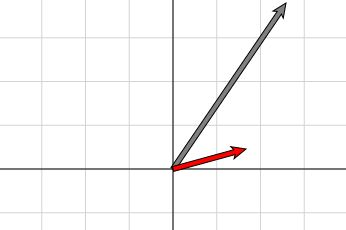
\includegraphics[width=\linewidth]{external/preview/simple-eigenvector-preview.jpg}
\end{sbspanel}%
\begin{sbspanel}{0.21}%
\noindent
\includegraphics[width=\linewidth]{generated/qrcode/interactive-simple-eigenvector.png}
\href{https://pretextbook.org/examples/sample-article/html/interactive-simple-eigenvector.html}{Standalone}%
\par
\href{https://pretextbook.org/examples/sample-article/html/interactive-simple-eigenvector-if.html}{Embed}%
\end{sbspanel}%
\end{sidebyside}%
\tcblower
\end{figureptx}%
\begin{inlineexercise}\label{interactive-html5-canvas-5}%
%
The interactive in \hyperref[figure-simple-eigenvector]{Figure~{\xreffont\ref{figure-simple-eigenvector}}} shows a vector \(\vec{x}\) in red, and the matrix-vector product \(A\vec{x}\) in grey, for a particular \(2\times 2\) matrix \(A\).  The four entries of the matrix \(A\) are coded into the interactive.  Can you deduce \(A\) simply by using the interactive?  Which theorem is the key?%
\end{inlineexercise}%
\begin{figureptx}{Figure}{Eigenvector demonstration}{figure-eigenvectors}{}%
\begin{sidebyside}{2}{0.075}{0.075}{0.17}%
\begin{sbspanel}{0.47}%
\noindent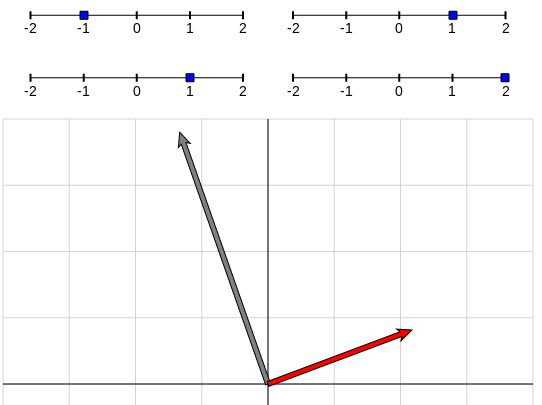
\includegraphics[width=\linewidth]{external/preview/eigenvectors-preview.jpg}
\end{sbspanel}%
\begin{sbspanel}{0.21}%
\noindent
\includegraphics[width=\linewidth]{generated/qrcode/interactive-eigenvectors.png}
\href{https://pretextbook.org/examples/sample-article/html/interactive-eigenvectors.html}{Standalone}%
\par
\href{https://pretextbook.org/examples/sample-article/html/interactive-eigenvectors-if.html}{Embed}%
\end{sbspanel}%
\end{sidebyside}%
\tcblower
\end{figureptx}%
The next example has ten \mono{<slate>} elements communicating with each other, and arranged with the layout features of a \mono{<sidebyside>} (see \hyperref[section-side-by-side]{Section~{\xreffont\ref{section-side-by-side}}}).%
\begin{figureptx}{Figure}{Affine Transformations}{figure-animation}{}%
\begin{sidebyside}{2}{0.075}{0.075}{0.17}%
\begin{sbspanel}{0.47}%
\noindent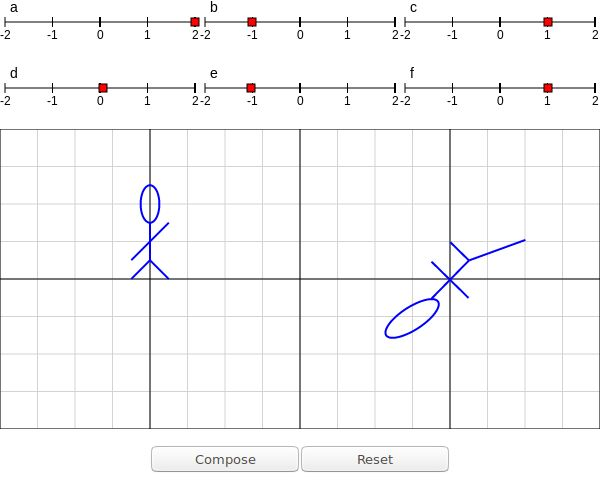
\includegraphics[width=\linewidth]{external/preview/animation-preview.jpg}
\end{sbspanel}%
\begin{sbspanel}{0.21}%
\noindent
\includegraphics[width=\linewidth]{generated/qrcode/interactive-animation.png}
\href{https://pretextbook.org/examples/sample-article/html/interactive-animation.html}{Standalone}%
\par
\href{https://pretextbook.org/examples/sample-article/html/interactive-animation-if.html}{Embed}%
\end{sbspanel}%
\end{sidebyside}%
\tcblower
\end{figureptx}%
\begin{warning}\label{interactive-html5-canvas-9}%
%
If your \mono{<interactive>} employs a \mono{<slate>} with a \mono{@surface} attribute whose value is \mono{html}, then you are advised to augment each top-level (\initialism{HTML}) element within the \mono{<slate>} with the attribute:%
\begin{codedisplay}
xmlns="http://www.w3.org/1999/xhtml"
\end{codedisplay}
This will identify \emph{all} of the elements within the \mono{<slate>} as \initialism{HTML} elements and not as PreTeXt elements.  The danger is that elements with the same name in both languages, such as \mono{<li>} and \mono{<table>}, will be mis-identified.  This could be harmless, but could also create chaos, such as disrupting numbering of PreTeXt elements.%
\par
See the source code of this document for examples:  \hyperref[figure-animation]{Figure~{\xreffont\ref{figure-animation}}} \hyperref[figure-interactive-slopes]{Figure~{\xreffont\ref{figure-interactive-slopes}}}, \hyperref[figure-piecewise]{Figure~{\xreffont\ref{figure-piecewise}}}.%
\par
Note that the \initialism{HTML} that is output can vary slightly from your source in small, harmless ways, such as empty (self-closing) elements being output with both an opening and a closing tag.  Please report any significant discrepancies.  Soon this requirement will be enforced in the code.%
\end{warning}
It is also possible to add \mono{<script>} elements within an interactive that contain properly escaped JS code. These elements will be placed at the end of the document created to hold the interactive content and can interactive with the other elements within the interactive but can not directly interact with the surrounding page.%
\par
Authors are strongly discouraged from trying to incorporate complex code in the form of a \mono{<script>}, but it can be a useful tool to call more complex code that is linked via \mono{@source} on the \mono{<interactive>}.%
\par
This example uses a \mono{<script>} to draw ``Hello World'' to a \mono{<slate>}%
\begin{figureptx}{Figure}{A simple embedded script example}{figure-simple-js-script}{}%
\begin{sidebyside}{2}{0.075}{0.075}{0.17}%
\begin{sbspanel}{0.47}%
\noindent
\includegraphics[width=\linewidth]{generated/preview/interactive-simple-js-script-preview.png}
\end{sbspanel}%
\begin{sbspanel}{0.21}%
\noindent
\includegraphics[width=\linewidth]{generated/qrcode/interactive-simple-js-script.png}
\href{https://pretextbook.org/examples/sample-article/html/interactive-simple-js-script.html}{Standalone}%
\par
\href{https://pretextbook.org/examples/sample-article/html/interactive-simple-js-script-if.html}{Embed}%
\end{sbspanel}%
\end{sidebyside}%
\tcblower
\end{figureptx}%
% end of subsection: HTML5 Canvas
%
%
\typeout{************************************************}
\typeout{Subsection 14.2 D3.js}
\typeout{************************************************}
%
\subsection{D3.js}\label{section-interactive-authored-8}%
\index{D3.js}%
\terminology{D3} is a Javascript library for ``Data-Driven Documents'', which might greatly enhance some data you wish to display.  In short, it uses the animation capabilities of \initialism{SVG}.  Available examples seem sensitive to the version of the library, so we have examples using different versions.  Use the \mono{@version} attribute on \mono{<interactive>} to specify the version number.  The default is \mono{5}.%
\par
The first example uses the force layout and collision detection from Version 3.  (The necessary commands are very different in Version 4.)  Pretend you are a working shepherding dog.  Can you separate, and catch, one of the herd?%
\par
This is adapted from a \href{https://bl.ocks.org/mbostock/3231298}{block}\footnote{\nolinkurl{bl.ocks.org/mbostock/3231298}\label{section-interactive-authored-8-5-2}} by \href{https://bl.ocks.org/mbostock}{Mike Bostock}\footnote{\nolinkurl{bl.ocks.org/mbostock}\label{section-interactive-authored-8-5-4}} with a \initialism{GPL} license.  A similar demonstration, only using an \initialism{HTML5} canvas is at \href{https://bl.ocks.org/mbostock/3231307}{\nolinkurl{bl.ocks.org/mbostock/3231307}}.%
\begin{figureptx}{Figure}{Force layout and collision detection}{section-interactive-authored-8-6}{}%
\begin{sidebyside}{2}{0.075}{0.075}{0.17}%
\begin{sbspanel}{0.47}%
\noindent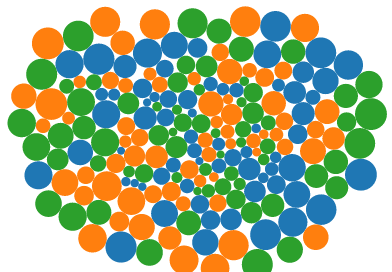
\includegraphics[width=\linewidth]{external/preview/collision-preview.png}
\end{sbspanel}%
\begin{sbspanel}{0.21}%
\noindent
\includegraphics[width=\linewidth]{generated/qrcode/interactive-d3-collision.png}
\href{https://pretextbook.org/examples/sample-article/html/interactive-d3-collision.html}{Standalone}%
\par
\href{https://pretextbook.org/examples/sample-article/html/interactive-d3-collision-if.html}{Embed}%
\end{sbspanel}%
\end{sidebyside}%
\tcblower
\end{figureptx}%
Similar, but different, this demonstration of a graph layout uses Version 4 of the library.  Technical notes:%
\begin{itemize}[label=\textbullet]
\item{}We have changed the size of the nodes, and their number, to fit in a smaller space.%
\item{}The Javascript script uses introspection to size itself, which would be a good general practice.%
\end{itemize}
%
\par
This is adapted from a \href{https://bl.ocks.org/shimizu/e6209de87cdddde38dadbb746feaf3a3}{block}\footnote{\nolinkurl{bl.ocks.org/shimizu/e6209de87cdddde38dadbb746feaf3a3}\label{section-interactive-authored-8-8-2}} by \href{https://bl.ocks.org/shimizu}{shimizu}\footnote{\nolinkurl{bl.ocks.org/shimizu}\label{section-interactive-authored-8-8-4}} with a \initialism{GPL} license.%
\begin{figureptx}{Figure}{Graph Layout}{section-interactive-authored-8-9}{}%
\begin{sidebyside}{2}{0.075}{0.075}{0.17}%
\begin{sbspanel}{0.47}%
\noindent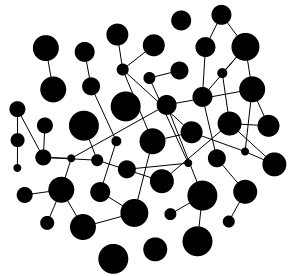
\includegraphics[width=\linewidth]{external/preview/graph-layout-preview.png}
\end{sbspanel}%
\begin{sbspanel}{0.21}%
\noindent
\includegraphics[width=\linewidth]{generated/qrcode/interactive-d3-graph-layout.png}
\href{https://pretextbook.org/examples/sample-article/html/interactive-d3-graph-layout.html}{Standalone}%
\par
\href{https://pretextbook.org/examples/sample-article/html/interactive-d3-graph-layout-if.html}{Embed}%
\end{sbspanel}%
\end{sidebyside}%
\tcblower
\end{figureptx}%
\begin{inlineexercise}[Graph Planarity]\label{section-interactive-authored-8-10}%
%
Can you move the vertices to new locations such that the resulting graph is planar?  (In other words, no edges cross?)%
\end{inlineexercise}%
Finally an example that actually uses some data.  Here is the description from the \href{https://bl.ocks.org/martinjc/7aa53c7bf3e411238ac8aef280bd6581}{original block}\footnote{\nolinkurl{bl.ocks.org/martinjc/7aa53c7bf3e411238ac8aef280bd6581}\label{section-interactive-authored-8-11-2}} by \href{https://bl.ocks.org/martinjc}{Martin Chorley}\footnote{\nolinkurl{bl.ocks.org/martinjc}\label{section-interactive-authored-8-11-4}} with an MIT License.%
\begin{quote}%
This visualisation uses a D3 force simulation to show the Twitter relationships between the Assembly Members in the Welsh Assembly in terms of the number of times each assembly member has mentioned another assembly member in a tweet.%
\par
Twitter relationships were mined on 22\slash{}03\slash{}2017, and are representative of the conversational relationships on that date. Links between AMs represent a conversational relationship: one AM has mentioned the other. Party colour indicates the direction of the mention.%
\par
Hover over the nodes to fade out non-connected nodes.%
\par
Rather than using intermediate nodes to create curved links (as in Mike Bostock's block), this adds curves by adding a calculated control point for each edge.%
\end{quote}
Technical notes:%
\begin{itemize}[label=\textbullet]
\item{}Once the nodes organize themselves (automatically in the beginning), they cannot be moved.%
\item{}We have adjusted the margins in an attempt to keep names visible on the right side, but without giving up too much space.%
\item{}We have adjust the repelling force, and the collision buffer, to better fit the available space.%
\item{}This example required its own \initialism{CSS}, which we have included as part of the \mono{<interactive>}.%
\item{}The data collected from the Twitter analysis is contained in a \initialism{JSON} file, \mono{mention\_network.json}, and where the script loads that file, it has a hardcoded path.  So this example is a bit brittle, should that file move.%
\end{itemize}
%
\begin{figureptx}{Figure}{Tweet mentions within the Welsh Assembly}{section-interactive-authored-8-14}{}%
\begin{sidebyside}{2}{0.075}{0.075}{0.17}%
\begin{sbspanel}{0.47}%
\noindent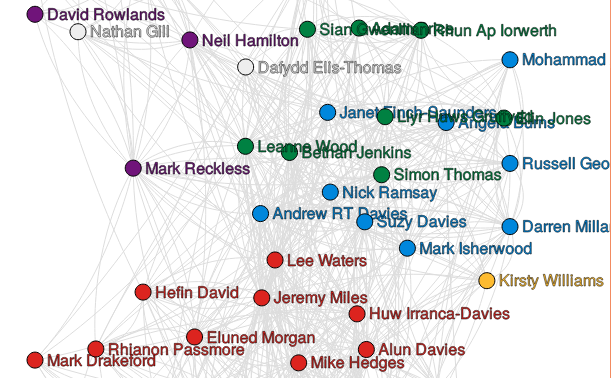
\includegraphics[width=\linewidth]{external/preview/welsh-assembly-preview.png}
\end{sbspanel}%
\begin{sbspanel}{0.21}%
\noindent
\includegraphics[width=\linewidth]{generated/qrcode/interactive-d3-welsh.png}
\href{https://pretextbook.org/examples/sample-article/html/interactive-d3-welsh.html}{Standalone}%
\par
\href{https://pretextbook.org/examples/sample-article/html/interactive-d3-welsh-if.html}{Embed}%
\end{sbspanel}%
\end{sidebyside}%
\tcblower
\end{figureptx}%
% end of subsection: D3.js
%
%
\typeout{************************************************}
\typeout{Subsection 14.3 SVG}
\typeout{************************************************}
%
\subsection{SVG}\label{svg-interactives}%
Entirely similar to using an HTML5 \mono{canvas} element (\hyperref[interactive-html5-canvas]{{\xreffont\ref{interactive-html5-canvas}}}), it is possible to control an \initialism{SVG} element with Javascript.  This example is from Mark McClure.%
\par
Look carefully at the source and rendering of this example as \initialism{HTML}.  The functions to choose from via radio buttons, and the change in \(x\), denoted later as \(h\), are being rendered as mathematics by the Javascript MathJax library.  However, this cannot be accomplished with simply \mono{\$...\$} nor by simply \mono{\textbackslash{}(...\textbackslash{})}, but instead by using the \mono{\textbackslash{}(...\textbackslash{})} and then also wrapping that in a \mono{<span>} element with a \mono{@class} attribute set to \mono{process-math}. (The latter is how we instruct MathJax as to which parts of a page to process, or not).  So to have MathJax render a nice \(x^2\) in this context (math inside \initialism{HTML} inside a \mono{<slate>} inside an \mono{<interactive>}) would be accomplished with%
\begin{codedisplay}
<span class="process-math">x^2</span>
\end{codedisplay}
%
\begin{figureptx}{Figure}{Tangent and secant slopes}{figure-interactive-slopes}{}%
\begin{sidebyside}{2}{0.075}{0.075}{0.17}%
\begin{sbspanel}{0.47}%
\noindent
\includegraphics[width=\linewidth]{generated/preview/interactive-slopes-preview.png}
\end{sbspanel}%
\begin{sbspanel}{0.21}%
\noindent
\includegraphics[width=\linewidth]{generated/qrcode/interactive-slopes.png}
\href{https://pretextbook.org/examples/sample-article/html/interactive-slopes.html}{Standalone}%
\par
\href{https://pretextbook.org/examples/sample-article/html/interactive-slopes-if.html}{Embed}%
\end{sbspanel}%
\end{sidebyside}%
\tcblower
\end{figureptx}%
\begin{inlineexercise}[Changing Secant Lines]\label{svg-interactives-5}%
%
When discussing the derivative as a limit, we think of the point of tangency as being fixed (the green point in \hyperref[figure-interactive-slopes]{{\xreffont\ref{figure-interactive-slopes}}}) and the ``other'' point defining the secant line as changing (the red point in \hyperref[figure-interactive-slopes]{{\xreffont\ref{figure-interactive-slopes}}}).  Switch it up!  Fix a large value of \(h\) (positive or negative) and then change the point of tangency (the green point).  Discuss what you observe.%
\end{inlineexercise}%
% end of subsection: SVG
%
%
\typeout{************************************************}
\typeout{Subsection 14.4 JSXGraph}
\typeout{************************************************}
%
\subsection{JSXGraph}\label{section-interactive-authored-10}%
\index{JSXGraph}%
\href{http://jsxgraph.uni-bayreuth.de/wp/index.html}{JSXGraph}\footnote{\nolinkurl{jsxgraph.uni-bayreuth.de}\label{section-interactive-authored-10-3-2}} is a ``cross-browser JavaScript library for interactive geometry, function plotting, charting, and data visualization in the web browser.''  Now a \mono{<slate>} will be what JSXGraph calls a \terminology{board}.  Again, you use Javascript to write onto a \mono{<slate>}, but have some powerful shortcuts available from the JSXGraph library.  For this reason, PreTeXt calls JSXGraph a ``language'', similar in may respects to how Sage is a language, but is really a Python library.  So realize that the syntax for using JSXGraph is that of Javascript.%
\par
Place Javascript inside a file that is specified with the \mono{@source} attribute of the \mono{<interactive>} element.  Then just be certain that \mono{@xml:id} of the \mono{<interactive>} element is passed as the \initialism{HTML} \mono{id} in an (early) call to JSXGraph's \mono{initBoard()} method.%
\par
The following example was contributed by Rick Roesler. The \mono{<figure>} is comprised of four \mono{<stack>} elements within a \mono{<sidebyside>}. By varying the time in the top box, the reader can observe the displacement, velocity, and acceleration of a ball thrown upward with an initial velocity of 30 m\slash{}s.%
\begin{figureptx}{Figure}{1-Dimensional Kinematics}{section-interactive-authored-10-6}{}%
\centering
\begin{image}{0.2}{0.6}{0.2}{}%

\includegraphics[width=\linewidth]{external/images/kinematics.png}
\end{image}%
\tcblower
\end{figureptx}%
The plot below is the curve \(r=a+b\theta\) in polar coordinates, for \(0\leq\theta\leq 8\pi\).  It may be manipulated with the sliders to control the shape of the curve.  Point \(A\) is contrained to the curve, but may be dragged to a new location. At \(A\) the tangent line and normal line are plotted as dashed red lines.  Use the controls in the lower left to adjust the viewing window.  This \href{http://jsxgraph.uni-bayreuth.de/wiki/index.php/Archimedean_spiral}{Archimedean Spiral}\footnote{\nolinkurl{jsxgraph.uni-bayreuth.de/wiki/index.php/Archimedean_spiral}\label{section-interactive-authored-10-7-6}} is taken from the \href{http://jsxgraph.uni-bayreuth.de/wiki/index.php/Category:Examples}{JSXGraph example wiki}\footnote{\nolinkurl{jsxgraph.uni-bayreuth.de/wiki/index.php/Category:Examples}\label{section-interactive-authored-10-7-8}}.  The code could be written in 7 lines.  Width is 80\% and aspect ratio is 4:3.%
\begin{figureptx}{Figure}{The Archimedian Spiral \(r = a + b\theta\), \(0\leq\theta\leq 8\pi\)}{section-interactive-authored-10-8}{}%
\index{Archimedian Spiral}%
\begin{sidebyside}{2}{0.075}{0.075}{0.17}%
\begin{sbspanel}{0.47}%
\noindent
\includegraphics[width=\linewidth]{generated/preview/interactive-archimedian-spiral-preview.png}
\end{sbspanel}%
\begin{sbspanel}{0.21}%
\noindent
\includegraphics[width=\linewidth]{generated/qrcode/interactive-archimedian-spiral.png}
\href{https://pretextbook.org/examples/sample-article/html/interactive-archimedian-spiral.html}{Standalone}%
\par
\href{https://pretextbook.org/examples/sample-article/html/interactive-archimedian-spiral-if.html}{Embed}%
\end{sbspanel}%
\end{sidebyside}%
\tcblower
\end{figureptx}%
Here is a more elaborate example, from the \href{http://jsxgraph.uni-bayreuth.de/showcase/}{JSXGraph Showcase}\footnote{\nolinkurl{jsxgraph.uni-bayreuth.de/showcase/}\label{section-interactive-authored-10-9-2}}, titled \href{http://jsxgraph.uni-bayreuth.de/showcase/infinity.html}{Infinity}\footnote{\nolinkurl{jsxgraph.uni-bayreuth.de/showcase/infinity.html}\label{section-interactive-authored-10-9-4}}.%
\par
There are two active sliders to control the shape and shading of the graphic, and hovering the mouse near one of the edges will highlight the entirety of one of the 30 quadrangles.  Finally, each of the four red corners may be dragged to a new location.  Code is 47 lines.  Width is 60\% and aspect ratio is the default, 1:1, i.e.\@ a square.%
\begin{figureptx}{Figure}{Infinity, from the JSXGraph Showcase}{section-interactive-authored-10-11}{}%
\begin{sidebyside}{2}{0.075}{0.075}{0.17}%
\begin{sbspanel}{0.47}%
\noindent
\includegraphics[width=\linewidth]{generated/preview/interactive-infinity-preview.png}
\end{sbspanel}%
\begin{sbspanel}{0.21}%
\noindent
\includegraphics[width=\linewidth]{generated/qrcode/interactive-infinity.png}
\href{https://pretextbook.org/examples/sample-article/html/interactive-infinity.html}{Standalone}%
\par
\href{https://pretextbook.org/examples/sample-article/html/interactive-infinity-if.html}{Embed}%
\end{sbspanel}%
\end{sidebyside}%
\tcblower
\end{figureptx}%
Here are the two new examples.  They have been included in a \mono{sidebyside} layout element with equal widths (see \hyperref[section-side-by-side]{Section~{\xreffont\ref{section-side-by-side}}}) so they can be placed horizontally across the page.  They are not wrapped as figures, so cannot be cross-referenced.  These are again from the \href{http://jsxgraph.uni-bayreuth.de/wiki/index.php/Category:Examples}{JSXGraph example wiki}\footnote{\nolinkurl{jsxgraph.uni-bayreuth.de/wiki/index.php/Category:Examples}\label{section-interactive-authored-10-12-4}}, the left being Fermat's Spiral and the right being a demonstration of B-splines.%
\begin{sidebyside}{2}{0.05}{0.05}{0.1}%
\end{sidebyside}%
\par
Finally, a piecewise function you can control, with traces of the domain values and range values in two other JSXGraph boards.  Boards and \initialism{HTML} buttons have been laid out using the \mono{sidebyside} layout element.%
\begin{figureptx}{Figure}{Piecewise Function}{figure-piecewise}{}%
\begin{sidebyside}{2}{0.075}{0.075}{0.17}%
\begin{sbspanel}{0.47}%
\noindent
\includegraphics[width=\linewidth]{generated/preview/interactive-piecewise-preview.png}
\end{sbspanel}%
\begin{sbspanel}{0.21}%
\noindent
\includegraphics[width=\linewidth]{generated/qrcode/interactive-piecewise.png}
\href{https://pretextbook.org/examples/sample-article/html/interactive-piecewise.html}{Standalone}%
\par
\href{https://pretextbook.org/examples/sample-article/html/interactive-piecewise-if.html}{Embed}%
\end{sbspanel}%
\end{sidebyside}%
\tcblower
\end{figureptx}%
Generally, we load an interactive into an HTML \mono{iframe} to sandbox (isolate) it from other interactives.  We does this for your own protection.  So, for example, one interactive cannot talk to another.  If two \mono{<slate>} need to communicate, then they are related, and should be placed into a single \mono{<interactive>}, allowed to layout themselves, or grouped within a \mono{<sidebyside>} allowing finer control.  Even if we have this under control, you might still enjoy reading \href{http://mikecavaliere.com/your-js-is-a-mess-javascript-namespacing/}{Your JS is a Mess}\footnote{\nolinkurl{mikecavaliere.com/your-js-is-a-mess-javascript-namespacing/}\label{section-interactive-authored-10-16-6}} at \mono{mikecavaliere.com/your-js-is-a-mess-javascript-namespacing/}.%
% end of subsection: JSXGraph
%
%
\typeout{************************************************}
\typeout{Subsection 14.5 JessieCode}
\typeout{************************************************}
%
\subsection{JessieCode}\label{section-interactive-authored-11}%
\index{JessieCode}%
\href{https://jsxgraph.uni-bayreuth.de/wp/docs_jessiecode/}{JessieCode}\footnote{\nolinkurl{jsxgraph.uni-bayreuth.de/wp/docs_jessiecode/}\label{section-interactive-authored-11-3-2}} is a scripting language for JSXGraph. It provides the core geometric and graphing features of JSXGraph without accessing the underlying JavaScript. In order to use JessieCode, you simply create the HTML \mono{<div>} element as you would for any other JSXGraph interactive plot and then provide the JessieCode script, which focuses on the geometric elements.%
\par
Because JessieCode is provided by JSXGraph, the interactive platform is \mono{jsxgraph}. The \mono{<slate>}, however, uses \mono{@surface} with value \mono{jessiecode}. The script can be embedded directly in your code. As usual, you would need to remember to escape the special characters. JessieCode uses \mono{<} and \mono{>} for inequalities as well as for declaring objects used to style geometric elements, and \mono{\&\&} is the boolean AND operator. Alternatively, you can provide the file as a separate resource, providing the URL with a \mono{@source} attribute. Attributes defining the JSXBoard at the time it is created should be included as attributes of the \mono{<slate>}, including \mono{@boundingbox}, \mono{@axis}, and \mono{@grid}.%
\par
For this first example, the JessieCode was included directly in the XML source as the contents of the associated slate.%
\begin{figureptx}{Figure}{Finding the Tangent Line of a Quadratic Function}{figure-quadratic-slope}{}%
\begin{sidebyside}{2}{0.075}{0.075}{0.17}%
\begin{sbspanel}{0.47}%
\noindent
\includegraphics[width=\linewidth]{generated/preview/interactive-quadratic-tangent-preview.png}
\end{sbspanel}%
\begin{sbspanel}{0.21}%
\noindent
\includegraphics[width=\linewidth]{generated/qrcode/interactive-quadratic-tangent.png}
\href{https://pretextbook.org/examples/sample-article/html/interactive-quadratic-tangent.html}{Standalone}%
\par
\href{https://pretextbook.org/examples/sample-article/html/interactive-quadratic-tangent-if.html}{Embed}%
\end{sbspanel}%
\end{sidebyside}%
\tcblower
\end{figureptx}%
For this second example, the JessieCode was included through an associated script file, loaded by the browser.%
\begin{figureptx}{Figure}{Graph of a function that is continuous but not differentiable at \(x=0\) because the slope of the secant line has no limit.}{figure-nondifferentiable-oscillation}{}%
\begin{sidebyside}{2}{0.075}{0.075}{0.17}%
\begin{sbspanel}{0.47}%
\noindent
\includegraphics[width=\linewidth]{generated/preview/interactive-oscillating-secant-preview.png}
\end{sbspanel}%
\begin{sbspanel}{0.21}%
\noindent
\includegraphics[width=\linewidth]{generated/qrcode/interactive-oscillating-secant.png}
\href{https://pretextbook.org/examples/sample-article/html/interactive-oscillating-secant.html}{Standalone}%
\par
\href{https://pretextbook.org/examples/sample-article/html/interactive-oscillating-secant-if.html}{Embed}%
\end{sbspanel}%
\end{sidebyside}%
\tcblower
\end{figureptx}%
% end of subsection: JessieCode
%
%
\typeout{************************************************}
\typeout{Subsection 14.6 Sage Interacts}
\typeout{************************************************}
%
\subsection{Sage Interacts}\label{section-interactive-authored-12}%
\index{Sage!interacts}%
Sage, and the Sage Cell Server, support interactive demonstrations, called \terminology{interacts}.%
\begin{itemize}[label=\textbullet]
\item{}The interactive elements are nearly trivial to construct.%
\item{}An interact is simply a single Python function (acted on by a decorator).%
\item{}You have the full mathematical power of Sage at your disposal, so can do some very powerful computations with high precision (or exactly).%
\item{}The interface is not as polished as what you can achieve with Javascript libraries.%
\item{}Graphics refresh with a round-trip to the server, so are not nearly as fluid as with other tools.%
\end{itemize}
Note that each interact is insulated from the others, unlike our other employment of the Sage Cell Server.%
\par
This example is by Marshall Hampton, taken from the \href{https://wiki.sagemath.org/interact/calculus}{Sage interact wiki}\footnote{\nolinkurl{wiki.sagemath.org/interact/calculus}\label{section-interactive-authored-12-4-2}}, specifically \href{https://wiki.sagemath.org/interact/calculus\#Numerical_integrals_with_the_midpoint_rule}{Numerical integrals with the midpoint rule}\footnote{\nolinkurl{wiki.sagemath.org/interact/calculus\#Numerical_integrals_with_the_midpoint_rule}\label{section-interactive-authored-12-4-4}}.%
\par
Also notice that when viewed in dark mode, this sample respects the rendering intent. That is due to \mono{@dark-mode-enabled} applied to it.%
\begin{figureptx}{Figure}{Numerical integrals using the midpoint rule}{figure-interactive-numerical-integral}{}%
\begin{sidebyside}{2}{0.075}{0.075}{0.17}%
\begin{sbspanel}{0.47}%
\noindent
\includegraphics[width=\linewidth]{generated/preview/interactive-numerical-integral-preview.png}
\end{sbspanel}%
\begin{sbspanel}{0.21}%
\noindent
\includegraphics[width=\linewidth]{generated/qrcode/interactive-numerical-integral.png}
\href{https://pretextbook.org/examples/sample-article/html/interactive-numerical-integral.html}{Standalone}%
\par
\href{https://pretextbook.org/examples/sample-article/html/interactive-numerical-integral-if.html}{Embed}%
\end{sbspanel}%
\end{sidebyside}%
\tcblower
\end{figureptx}%
% end of subsection: Sage Interacts
%
%
\typeout{************************************************}
\typeout{Subsection 14.7 Geogebra}
\typeout{************************************************}
%
\subsection{Geogebra}\label{section-interactive-authored-13}%
To embed a GeoGebra applet as-is from GeoGebra's Classroom Resources site (by material ID), see \hyperref[subsection-geogebra-server]{Subsection~{\xreffont\ref{subsection-geogebra-server}}}. To design your own applet (either from scratch, or modifying something that already exists in one of those three forms) you may use one of Geogebra's ``Apps'' to embed the material in your document. (But note, use of the App comes with licensing restrictions.) PreTeXt will handle most of the technical details for you.%
\par
Do one of the following:%
\begin{enumerate}
\item{}Identify a material ID from GeoGebra's Classroom Resources site. You might even make the material yourself on that site.%
\item{}Obtain a \mono{.ggb} file from GeoGebra. You might construct something on a desktop installation of GeoGebra and save it. If you have a base64-encoded string for a GeoGebra applet, but you don't have a \mono{.ggb} file, you can decode the string and save the result. For example, at \href{https://www.opinionatedgeek.com/codecs/base64decoder}{\nolinkurl{https://www.opinionatedgeek.com/codecs/base64decoder}}.%
\item{}Obtain a base64 encoded string for a GeoGebra applet. You might first open a \mono{.ggb} file in a desktop installation of GeoGebra, and push ctrl-shift-B (command-shift-B on a Mac) and then the string will be in your clipboard.%
\item{}None of the above, with the intention to make an applet from scratch.%
\end{enumerate}
%
\par
Then mimic the examples that follow, using GeoGebra API commands documented at \href{https://wiki.geogebra.org/en/Reference:GeoGebra_Apps_API}{Geogebra API Manual}\footnote{\nolinkurl{wiki.geogebra.org/en/Reference:GeoGebra_Apps_API}\label{section-interactive-authored-13-4-2}}, but do not include the \mono{ggbApplet.} or \mono{applet.} used in examples to prefix the functions\textemdash{}that part of the code will be provided automatically by PreTeXt.%
\par
Jack Green created an applet on the Classroom Resources site with ID \mono{D4s2v4ft}, which you may view at \href{https://www.geogebra.org/m/D4s2v4ft}{\nolinkurl{www.geogebra.org/m/D4s2v4ft}}. Suppose you would like to use this in your project, but change something about it. We will change something trivial, making the \(y\)-axis ticks be separated \(5\) apart instead of \(10\) apart. We also decide we want a different aspect ratio and overall width. One gotcha: the original applet is loaded and then PreTeXt uses \mono{@width} and \mono{@aspect} attributes to resize the viewing window using the top left corner as an anchor. This does not rescale axes and that may leave you with important elements missing from the viewing window. So here we reset the viewing window to return to values that are in the original. Lastly, we disable zooming, which is not helpful for this applet. To do each of these things, we rely on the GeoGebra API manual at \href{https://wiki.geogebra.org/en/Reference:GeoGebra_Apps_API}{Geogebra API Manual}\footnote{\nolinkurl{wiki.geogebra.org/en/Reference:GeoGebra_Apps_API}\label{section-interactive-authored-13-5-10}}. It is important to use one command per line.%
\begin{figureptx}{Figure}{GeoGebra: modified material ID}{section-interactive-authored-13-6}{}%
\begin{sidebyside}{2}{0.075}{0.075}{0.17}%
\begin{sbspanel}{0.47}%
\noindent
\includegraphics[width=\linewidth]{generated/preview/geogebra-train-distance-preview.png}
\end{sbspanel}%
\begin{sbspanel}{0.21}%
\noindent
\includegraphics[width=\linewidth]{generated/qrcode/geogebra-train-distance.png}
\href{https://pretextbook.org/examples/sample-article/html/geogebra-train-distance.html}{Standalone}%
\par
\href{https://pretextbook.org/examples/sample-article/html/geogebra-train-distance-if.html}{Embed}%
\end{sbspanel}%
\end{sidebyside}%
\tcblower
\end{figureptx}%
The same can be done with a \mono{.ggb} file. Here we use two provided by David Rosoff, and one provided by Tevian Dray. The path to the file needs to be relative. First, David's original.%
\begin{figureptx}{Figure}{GeoGebra: \mono{.ggb} file}{section-interactive-authored-13-8}{}%
\begin{sidebyside}{2}{0.075}{0.075}{0.17}%
\begin{sbspanel}{0.47}%
\noindent
\includegraphics[width=\linewidth]{generated/preview/geogebra-astroid-original-preview.png}
\end{sbspanel}%
\begin{sbspanel}{0.21}%
\noindent
\includegraphics[width=\linewidth]{generated/qrcode/geogebra-astroid-original.png}
\href{https://pretextbook.org/examples/sample-article/html/geogebra-astroid-original.html}{Standalone}%
\par
\href{https://pretextbook.org/examples/sample-article/html/geogebra-astroid-original-if.html}{Embed}%
\end{sbspanel}%
\end{sidebyside}%
\tcblower
\end{figureptx}%
Now we modify David's applet in a few ways.%
\begin{figureptx}{Figure}{GeoGebra: modified from \mono{.ggb} file}{section-interactive-authored-13-10}{}%
\begin{sidebyside}{2}{0.075}{0.075}{0.17}%
\begin{sbspanel}{0.47}%
\noindent
\includegraphics[width=\linewidth]{generated/preview/geogebra-astroid-preview.png}
\end{sbspanel}%
\begin{sbspanel}{0.21}%
\noindent
\includegraphics[width=\linewidth]{generated/qrcode/geogebra-astroid.png}
\href{https://pretextbook.org/examples/sample-article/html/geogebra-astroid.html}{Standalone}%
\par
\href{https://pretextbook.org/examples/sample-article/html/geogebra-astroid-if.html}{Embed}%
\end{sbspanel}%
\end{sidebyside}%
\tcblower
\end{figureptx}%
\begin{figureptx}{Figure}{GeoGebra: modified from \mono{.ggb} file}{section-interactive-authored-13-11}{}%
\begin{sidebyside}{2}{0.075}{0.075}{0.17}%
\begin{sbspanel}{0.47}%
\noindent
\includegraphics[width=\linewidth]{generated/preview/geogebra-cycloid-preview.png}
\end{sbspanel}%
\begin{sbspanel}{0.21}%
\noindent
\includegraphics[width=\linewidth]{generated/qrcode/geogebra-cycloid.png}
\href{https://pretextbook.org/examples/sample-article/html/geogebra-cycloid.html}{Standalone}%
\par
\href{https://pretextbook.org/examples/sample-article/html/geogebra-cycloid-if.html}{Embed}%
\end{sbspanel}%
\end{sidebyside}%
\tcblower
\end{figureptx}%
In this one provided by Tevian Dray, we make no modifications (except for those imposed by the scaling). You will need to zoom out a bit, and then pan over some, to see all the pieces.%
\begin{figureptx}{Figure}{GeoGebra: a constructive ``proof'' that SAS congruence holds in Euclidean geometry (from Tevian Dray)}{section-interactive-authored-13-13}{}%
\begin{sidebyside}{2}{0.075}{0.075}{0.17}%
\begin{sbspanel}{0.47}%
\noindent
\includegraphics[width=\linewidth]{generated/preview/geogebra-SAS-preview.png}
\end{sbspanel}%
\begin{sbspanel}{0.21}%
\noindent
\includegraphics[width=\linewidth]{generated/qrcode/geogebra-SAS.png}
\href{https://pretextbook.org/examples/sample-article/html/geogebra-SAS.html}{Standalone}%
\par
\href{https://pretextbook.org/examples/sample-article/html/geogebra-SAS-if.html}{Embed}%
\end{sbspanel}%
\end{sidebyside}%
\tcblower
\end{figureptx}%
You could also use a base64-encoded string of the \mono{.ggb} file. You might come across such a string somewhere, or you might generate one by opening a \mono{.ggb} file in a desktop installation of GeoGebra, and pushing ctrl-shift-B (command-shift-B on a Mac) to get the string in your clipboard. If you do this, you could use a \mono{@base64} attribute in place of the \mono{@source} attribute in the previous example. We don't do that here because such a string is generally over 5000 characters long and we are keeping the sample article source a bit cleaner.%
\par
The next example shows how you can communicate between a GeoGebra applet and a \mono{<slate>} contained in the interactive.  The process is mediated by javascript code specified in the \mono{@source} attribute of the interactive.  Event listeners in the code update the HTML when the diagram changes or vice-versa.  MathJax is also notified when it needs to update math.%
\par
Note that this example has a \mono{<slate>} whose \mono{@surface} is \mono{pretext} \emph{and} a \mono{<slate>} whose \mono{@surface} is \mono{html}, the latter requiring a namespace declaration.  The former produces HTML according to the PreTeXt templates, which is fairly predictable, but never guaranteed to always be identical over time.  A PreTeXt slate uses familiar syntax, produces results styled consistently, but might break in the future.  While an HTML slate is similar, the results will not be styled, but it does allow for a wider range of HTML elements (a \mono{button} element here) and will not change over time.%
\par
The indefinite integral in the last row of the table is a gratuitious test that aurhors' macros from \mono{<docinfo>} are available to MathJax.  Finally, a PreTeXt slate will only recognize \mono{<p>}, \mono{<tabular>}, \mono{<sidebyside>}, and \mono{<sbsgroup>} as children.  Make a feature request if you have a good case for more.%
\begin{figureptx}{Figure}{Geogebra\slash{}PreTeXt Communications}{figure_Interactive-3d-direction-vector}{}%
\begin{sidebyside}{2}{0.075}{0.075}{0.17}%
\begin{sbspanel}{0.47}%
\noindent
\includegraphics[width=\linewidth]{generated/preview/ggb_3d-direction-vector_interactive-preview.png}
\end{sbspanel}%
\begin{sbspanel}{0.21}%
\noindent
\includegraphics[width=\linewidth]{generated/qrcode/ggb_3d-direction-vector_interactive.png}
\href{https://pretextbook.org/examples/sample-article/html/ggb_3d-direction-vector_interactive.html}{Standalone}%
\par
\href{https://pretextbook.org/examples/sample-article/html/ggb_3d-direction-vector_interactive-if.html}{Embed}%
\end{sbspanel}%
\end{sidebyside}%
\tcblower
\end{figureptx}%
Lastly, you may just wish to build something from scratch using GeoGebra API. Note that for accessibilty reasons, some objects are rendered unselectable with the \mono{setFixed} command. Perhaps this should have been done with the previous examples, but that is more difficult when you do not know all of their names. Note that the GeoGebra scripting command \mono{setAttribute} also changes the webpage's focus, so it is better to set the perspective using an attribute of the slate.%
\begin{figureptx}{Figure}{GeoGebra: from scratch}{section-interactive-authored-13-20}{}%
\begin{sidebyside}{2}{0.075}{0.075}{0.17}%
\begin{sbspanel}{0.47}%
\noindent
\includegraphics[width=\linewidth]{generated/preview/geogebra-seed-head-preview.png}
\end{sbspanel}%
\begin{sbspanel}{0.21}%
\noindent
\includegraphics[width=\linewidth]{generated/qrcode/geogebra-seed-head.png}
\href{https://pretextbook.org/examples/sample-article/html/geogebra-seed-head.html}{Standalone}%
\par
\href{https://pretextbook.org/examples/sample-article/html/geogebra-seed-head-if.html}{Embed}%
\end{sbspanel}%
\end{sidebyside}%
\tcblower
\end{figureptx}%
% end of subsection: Geogebra
%
%
\typeout{************************************************}
\typeout{Subsection 14.8 CircuitJS}
\typeout{************************************************}
%
\subsection{CircuitJS}\label{section-interactive-authored-14}%
\href{https://www.falstad.com/circuit/}{CircuitJS}\footnote{\nolinkurl{www.falstad.com/circuit}\label{section-interactive-authored-14-2-2}} is an electronic circuit simulator.  A circuit can be described by a language, which PreTeXt will interpret and submit for rendering.  The next two examples are identical, but provided in slightly different ways, see the PreTeXt source for more.  Preview images for PDF will be added later.%
\begin{figureptx}{Figure}{CircuitJS Example (source via an encoded attribute)}{figure-circuitjs-attribute}{}%
\begin{sidebyside}{2}{0.075}{0.075}{0.17}%
\begin{sbspanel}{0.47}%
\noindent
\includegraphics[width=\linewidth]{generated/preview/interactive-circuitjs-attribute-preview.png}
\end{sbspanel}%
\begin{sbspanel}{0.21}%
\noindent
\includegraphics[width=\linewidth]{generated/qrcode/interactive-circuitjs-attribute.png}
\href{https://pretextbook.org/examples/sample-article/html/interactive-circuitjs-attribute.html}{Standalone}%
\end{sbspanel}%
\end{sidebyside}%
\tcblower
\end{figureptx}%
\begin{figureptx}{Figure}{CircuitJS Example (source authored directly)}{figure-circuitjs}{}%
\begin{sidebyside}{2}{0.075}{0.075}{0.17}%
\begin{sbspanel}{0.47}%
\noindent
\includegraphics[width=\linewidth]{generated/preview/interactive-circuitjs-preview.png}
\end{sbspanel}%
\begin{sbspanel}{0.21}%
\noindent
\includegraphics[width=\linewidth]{generated/qrcode/interactive-circuitjs.png}
\href{https://pretextbook.org/examples/sample-article/html/interactive-circuitjs.html}{Standalone}%
\end{sbspanel}%
\end{sidebyside}%
\tcblower
\end{figureptx}%
% end of subsection: CircuitJS
%
%
\typeout{************************************************}
\typeout{Subsection 14.9 IFrames from Files}
\typeout{************************************************}
%
\subsection{IFrames from Files}\label{interactive-iframes-local}%
An \mono{iframe} is an \initialism{HTML} element that allows embedding of a complete web page within another one.  Here we use this device to provide interactive 3D diagrams built with other tools.%
\par
We begin with a Jupyter notebook hosted on \href{https://cocalc.com}{\nolinkurl{CoCalc.com}}.  News of success on other hosts for Jupyter notebook servers will allow us to expand this description.  We use a Sage kernel and create a 3D surface suggested by Juan Carlos Bustamante:%
\begin{codedisplay}
var('x,y')
plot3d(x^2 - y^2, (x,-1,1), (y,-1,1), color="orange", mesh=true)
\end{codedisplay}
News of other computational engines that produce similar graphics will also allow us to further expand this description.  Note that for the case of Sage 3D plots, support for the \mono{<sageplot>} element makes this even easier.  For example, see \hyperref[figure-sage-implicit-surface]{{\xreffont\ref{figure-sage-implicit-surface}}}.%
\par
A button in the lower right allows for several options, one is \mono{Save as HTML}, which will produce a complete self-contained web page we can recycle.  We save this file with our other externally-created images, in a directory that we choose to name \mono{iframe}\textemdash{}you can use another name.  Then we make an \mono{<interactive>} with an \mono{@iframe} attribute that has the filename, starting from \mono{iframe/} (in other words, do not include the name of your managed directory of external images).%
\begin{figureptx}{Figure}{Sage+Jupyter \mono{iframe}}{figure-sage-jupyter-iframe}{}%
\begin{sidebyside}{2}{0.075}{0.075}{0.17}%
\begin{sbspanel}{0.47}%
\noindent
\includegraphics[width=\linewidth]{generated/preview/interactive-sage-jupyter-iframe-preview.png}
\end{sbspanel}%
\begin{sbspanel}{0.21}%
\noindent
\includegraphics[width=\linewidth]{generated/qrcode/interactive-sage-jupyter-iframe.png}
\href{https://pretextbook.org/examples/sample-article/html/interactive-sage-jupyter-iframe.html}{Standalone}%
\end{sbspanel}%
\end{sidebyside}%
\tcblower
\end{figureptx}%
Note that the downloaded file has links to specific versions of the \mono{three.js} library, which are beyond our control, and beyond your control.  So there is a future where these images may need updating.  You could put your source code into a (large) comment with your project's source for safe-keeping in the future.  See \hyperref[interactive-iframes-server]{Subsection~{\xreffont\ref{interactive-iframes-server}}} for the server version.%
% end of subsection: IFrames from Files
%
%
\typeout{************************************************}
\typeout{Subsection 14.10 threejs}
\typeout{************************************************}
%
\subsection{threejs}\label{interactive-threejs}%
Once upon a time there was an example here using the \mono{threejs} 3D Javascript library.  It was \href{https://threejs.org/examples/\#webgl_geometry_extrude_splines}{one of the project's examples}\footnote{\nolinkurl{threejs.org/examples/\#webgl_geometry_extrude_splines}\label{interactive-threejs-2-3}}, licensed with an MIT License, with minimal modifications.%
\par
But it would seem to have become a bit more complicated to embed and our example was not rendering.  As of 2022-08-08, we have removed it.  Of course, you can find it in the git repository, perhaps searching on the date string just mentioned.  It woulld be interesting to see if our \mono{<interactive>} framework could still support the changes.%
\par
The following two examples are meant to be instructive (\emph{only}).  The end result is accomplished in a much more straightforward way be the method in \hyperref[interactive-iframes-local]{Subsection~{\xreffont\ref{interactive-iframes-local}}}.  We illustrate a way to get a \mono{three.js} image out of an \initialism{HTML} page as a Javascript file and render it on a PreTeXt \mono{<slate>}.  We follow the second method in a \href{https://golem.ph.utexas.edu/category/2017/12/sagemath_and_3d_models_in_webp.html}{blog post from the \(n\)-Category Cafe}\footnote{\nolinkurl{golem.ph.utexas.edu/category/2017/12/sagemath_and_3d_models_in_webp.html}\label{interactive-threejs-4-8}}.%
\begin{enumerate}
\item{}Open a Jupyter Notebook that utilizes a Sage kernel.  This can be done easily at \href{https://cocalc.com}{CoCalc}\footnote{\nolinkurl{cocalc.com}\label{interactive-threejs-4-9-1-2}} (and for free initially).%
\item{}Sketch a surface using Sage code.  We recycle the suggestion from Juan Carlos Bustamante in \hyperref[interactive-iframes-local]{Subsection~{\xreffont\ref{interactive-iframes-local}}}:%
\begin{codedisplayleft}
var('x,y')
plot3d(x^2 - y^2, (x,-1,1), (y,-1,1), color="orange", mesh=true)
\end{codedisplayleft}
%
\item{}Look for a button (in the lower-right) which will provide a menu option \mono{Save as HTML}.  Save the resulting \initialism{HTML} file, and open a \emph{copy} in a text editor.%
\item{}You are now looking for two \initialism{HTML} \mono{script} elements.  One will tell you just which version of \mono{three.js} is being used, vis a \mono{@src} attribute.  For the second example below we located%
\begin{codedisplay}
https://cdn.jsdelivr.net/gh/sagemath/threejs-sage@r122/build/three.min.js
\end{codedisplay}
The \mono{@r122} will likely be a version number, which is a good thing for the longevity of your work.  This will get used in the \mono{@source} attribute of your \mono{<interactive>}, which will have \mono{@platform} set to \mono{javascript}.%
\par
The second \mono{script} element is likely huge and has many generic functions defined it.  There may be a huge variable full of data points computed by Sage.  Copy the \emph{contents} of this \mono{script} element into a new Javascript file (so use a \mono{.js} extension).  Do not edit in any way until you read further.  Once adjusted, this file too gets specified in the \mono{@source} attribute of your \mono{<interactive>}.%
\item{}Your \mono{<interactive>} needs a \mono{<slate>} element for the graphic to draw on, and you will need to give it a proper \mono{@xml:id} attribute, plus teh \mono{@surface} will be set to \mono{div}.  Then you need to edit the Javascript file to connect the graphic with the slate, via IDs in your PreTeXt source and on teh \initialism{HTML} \mono{div} created by the slate.  Look at the provided examples to see how.  Do not make any other edits to this file, even if tempted.%
\item{}Study the two examples below, and mimic how they were constructed.%
\end{enumerate}
%
\par
First, the example given in the blog post referenced above.%
\begin{figureptx}{Figure}{\mono{threejs} catenoid surface, from \(n\)-Category Cafe}{figure-threejs-catenoid-surface}{}%
\begin{sidebyside}{2}{0.075}{0.075}{0.17}%
\begin{sbspanel}{0.47}%
\noindent
\includegraphics[width=\linewidth]{generated/preview/interactive-threejs-catenoid-surface-preview.png}
\end{sbspanel}%
\begin{sbspanel}{0.21}%
\noindent
\includegraphics[width=\linewidth]{generated/qrcode/interactive-threejs-catenoid-surface.png}
\href{https://pretextbook.org/examples/sample-article/html/interactive-threejs-catenoid-surface.html}{Standalone}%
\par
\href{https://pretextbook.org/examples/sample-article/html/interactive-threejs-catenoid-surface-if.html}{Embed}%
\end{sbspanel}%
\end{sidebyside}%
\tcblower
\end{figureptx}%
Second, the example from JC Bustamante.%
\begin{figureptx}{Figure}{\mono{threejs} saddle by Sage}{figure-threejs-saddle}{}%
\begin{sidebyside}{2}{0.075}{0.075}{0.17}%
\begin{sbspanel}{0.47}%
\noindent
\includegraphics[width=\linewidth]{generated/preview/interactive-threejs-saddle-preview.png}
\end{sbspanel}%
\begin{sbspanel}{0.21}%
\noindent
\includegraphics[width=\linewidth]{generated/qrcode/interactive-threejs-saddle.png}
\href{https://pretextbook.org/examples/sample-article/html/interactive-threejs-saddle.html}{Standalone}%
\par
\href{https://pretextbook.org/examples/sample-article/html/interactive-threejs-saddle-if.html}{Embed}%
\end{sbspanel}%
\end{sidebyside}%
\tcblower
\end{figureptx}%
% end of subsection: threejs
%
%
\typeout{************************************************}
\typeout{Subsection 14.11 DoenetML}
\typeout{************************************************}
%
\subsection{DoenetML}\label{interactive-doenetml}%
\href{https://doenet.org}{DoenetML}\footnote{\nolinkurl{doenet.org}\label{interactive-doenetml-2-2}} is a markup language inspired by PreTeXt for semantically describing interactive mathematics applets for the web. Use \mono{interactive[@platform=\textquotedbl{}doenetml\textquotedbl{}]} with a \mono{slate[@surface=\textquotedbl{}doenetml\textquotedbl{}]} to include DoenetML content within your document.%
\par
Since DoenetML is similar to, but not completely compatible with, XML, it cannot be authored directly within a PreTeXt document without painstakingly escaping every \mono{<} as \mono{\&lt;} and every \mono{\&} as \mono{\&amp;}. However, a convenient workflow to avoid this is to author your DoenetML in a separate file like \mono{example.doenetml}, then include this file within your PreTeXt document using \mono{<xi:include parse=\textquotedbl{}text\textquotedbl{} href=\textquotedbl{}path/to/example.doenetml\textquotedbl{}/>}.%
\begin{figureptx}{Figure}{DoenetML example}{figure-doenetml}{}%
\begin{sidebyside}{2}{0.075}{0.075}{0.17}%
\begin{sbspanel}{0.47}%
\noindent
\includegraphics[width=\linewidth]{generated/preview/interactive-doenetml-example-preview.png}
\end{sbspanel}%
\begin{sbspanel}{0.21}%
\noindent
\includegraphics[width=\linewidth]{generated/qrcode/interactive-doenetml-example.png}
\href{https://pretextbook.org/examples/sample-article/html/interactive-doenetml-example.html}{Standalone}%
\par
\href{https://pretextbook.org/examples/sample-article/html/interactive-doenetml-example-if.html}{Embed}%
\end{sbspanel}%
\end{sidebyside}%
\tcblower
\end{figureptx}%
% end of subsection: DoenetML
% end of section: Interactive Elements, Authored in Javascript
%
%
\typeout{************************************************}
\typeout{Section 15 Interactive Elements, Server}
\typeout{************************************************}
%
\section{Interactive Elements, Server}\label{section-interactive-server}%
\index{interactive elements!server}%
\index{embedded interactive elements!server}%
% Introduction
When outputting Web page versions, it is possible to embed a variety of dynamic interactive elements.  In a \LaTeX{}\slash{}PDF version, these will necessarily need to be replaced by some static substitute, such as a screenshot.  See \hyperref[section-sage-cells]{Section~{\xreffont\ref{section-sage-cells}}} for the specifics of embedding instances of the Sage Cell Server, which is more elaborate, and not entirely similar.%
\par
Interactives in this section have code that lives on a server somewhere (in the ``cloud'').  So maybe you uploaded an interactive demonstration, or maybe somebody else did.  In this sense, these are easier to create or use.  But pay attention, the code may come with restrictive licenses, even if you are the author originally.  See \hyperref[section-interactive-authored]{Section~{\xreffont\ref{section-interactive-authored}}} for more interactives that can be free as in ``freedom'' or \textit{liberté}.  CalcPlot3D is the notable exception here.%
\par
(2018-06-22) Almost everything in this section is under active development and not stable yet.  Feel free to experiment and make suggestions and requests.  This page takes a while to completely load, so be patient.%
% end of introduction
%
%
\typeout{************************************************}
\typeout{Subsection 15.1 GeoGebra}
\typeout{************************************************}
%
\subsection{GeoGebra}\label{subsection-geogebra-server}%
\index{Geogebra!server}%
\index{Geogebra!material}%
A Geogebra \terminology{material} is something you might use in a class.  It could also be called an interactive demonstration.  Go browsing at \href{https://www.geogebra.org/materials/}{\nolinkurl{www.geogebra.org/materials/}} and find something appropriate for your project.  Or make an account and create your own.%
\par
Once you find a material that looks instructive, it will be at a \initialism{URL} such as%
\begin{codedisplay}
https://www.geogebra.org/m/KGn2d4Qd
\end{codedisplay}
and you want to pick off the identifier on the end, in this case \mono{KGn2d4Qd}.  Then author%
\begin{codedisplay}
<interactive geogebra="KGn2d4Qd" />
\end{codedisplay}
At this writing (2018-02-04) you will want to place this inside a \mono{figure}, with a caption, as we do right now with material \mono{KGn2d4Qd}.%
\par
The shape of the material will be fixed, so guess (or measure with an on-screen ruler), the aspect ratio and use that in the \mono{<interactive>} element. If the width of the original material is anything other than 800 pixels, you should add \mono{@material-width} with the actual material width (units are pixels).%
\begin{figureptx}{Figure}{Right Triangle Paradox}{subsection-geogebra-server-7}{}%
\begin{sidebyside}{2}{0.075}{0.075}{0.17}%
\begin{sbspanel}{0.47}%
\noindent
\includegraphics[width=\linewidth]{generated/preview/geogebra-right-triangle-preview.png}
\end{sbspanel}%
\begin{sbspanel}{0.21}%
\noindent
\includegraphics[width=\linewidth]{generated/qrcode/geogebra-right-triangle.png}
\href{https://pretextbook.org/examples/sample-article/html/geogebra-right-triangle.html}{Standalone}%
\end{sbspanel}%
\end{sidebyside}%
\tcblower
\end{figureptx}%
There are some optional control elements that Geogebra provides, such as the presence of the toolbar and the reset button. These can be controlled by adding the following additional attributes to the \mono{interactive}.%
\begin{itemize}[label=\textbullet]
\item{}\mono{toolbar=\textquotedbl{}yes\textquotedbl{}}: add the Geogebra toolbar above the material%
\item{}\mono{algebra-input=\textquotedbl{}yes\textquotedbl{}}: add an entry box below the material to add graphical objects using algebra formulas or Geogebra graphical commands%
\item{}\mono{reset-icon=\textquotedbl{}yes\textquotedbl{}}: enable the reset icon%
\item{}\mono{shift-drag-zoom=\textquotedbl{}yes\textquotedbl{}}: enable ability to drag and zoom the viewing context%
\end{itemize}
%
\par
Note that materials hosted at \mono{geogebra.org} have a non-standard, non-commercial license you must agree to before you can download them as source code.  Perhaps you must forfeit your copyright when you upload a material?  We have not investigated this thoroughly.%
% end of subsection: GeoGebra
%
%
\typeout{************************************************}
\typeout{Subsection 15.2 Desmos Graphs}
\typeout{************************************************}
%
\subsection{Desmos Graphs}\label{section-interactive-server-6}%
\index{Desmos graphs}%
\terminology{Desmos} provides interactive graphing applications.  The following example was created by Ann Cary and made available via the ``Share'' function of Desmos.  You can make your own Desmos graph, choose the ``Share'' icon, and the ``Embed'' option, to get a \initialism{URL} such as%
\begin{codedisplay}
https://www.desmos.com/calculator/ttox1bvxku
\end{codedisplay}
You want to pick off the identifier on the end, in this case \mono{ttox1bvxku}, then author%
\begin{codedisplay}
<interactive desmos="ttox1bvxku" width="60%" aspect="2:3" />
\end{codedisplay}
as we have done here.%
\par
The static image employed in the \LaTeX{} version of this article was obtained by viewing the graph at the Desmos site (i.e.\@, not the embedded version in the PreTeXt HTML version), and using the Share button to export a \initialism{PNG} image.  In this case, we used a ``Medium Rectangle'' and ``Thick'' lines.%
\begin{figureptx}{Figure}{Graph of \(ln(x^2+5)-3\)}{section-interactive-server-6-5}{}%
\begin{sidebyside}{2}{0.075}{0.075}{0.17}%
\begin{sbspanel}{0.47}%
\noindent
\includegraphics[width=\linewidth]{generated/preview/desmos-natural-log-preview.png}
\end{sbspanel}%
\begin{sbspanel}{0.21}%
\noindent
\includegraphics[width=\linewidth]{generated/qrcode/desmos-natural-log.png}
\href{https://pretextbook.org/examples/sample-article/html/desmos-natural-log.html}{Standalone}%
\end{sbspanel}%
\end{sidebyside}%
\tcblower
\end{figureptx}%
Note that Desmos has extensive \pubtitle{Terms of Service} which include restrictions on commercial uses.%
% end of subsection: Desmos Graphs
%
%
\typeout{************************************************}
\typeout{Subsection 15.3 CalcPlot3D}
\typeout{************************************************}
%
\subsection{CalcPlot3D}\label{section-interactive-server-7}%
\index{CalcPlot3D}%
CalcPlot3D is a Javascript application for creating, visualizing, and understanding plots of 3D surfaces.  So it would be an ideal companion to a book on multivariate calculus, but should be useful in other courses of study.%
\par
To use it, start at the \href{https://c3d.libretexts.org/CalcPlot3D/index.html}{online app version}\footnote{\nolinkurl{c3d.libretexts.org/CalcPlot3D/index.html}\label{section-interactive-server-7-4-2}}.  Create a plot and adjust the image to a viewpoint and scale if you like.  Then, click the menu\slash{}hamburger icon in the upper-left and choose \mono{File}.  From here you can save a \initialism{PNG} image for the static version, but you also want to select \mono{Encode View in URL}.  Now your browser address bar is filled with a query string (\emph{all} the stuff \emph{after} the question-mark) that has all the information necessary to reproduce your plot (and view).  Copy everything after the first question-mark to the \mono{interactive/code} element.  Be sure to replace any ampersands by \mono{\&amp;} (see the Author's Guide for more about certain characters in \initialism{URL}s).  Examine the source for the examples below to see how they are authored.  The \pubtitle{Help Manual} for CalcPlot3D is also available off the menu\slash{}hamburger icon in the upper-left.%
\par
In \hyperref[figure-intersecting-planes]{Figure~{\xreffont\ref{figure-intersecting-planes}}} grab the image with your mouse and rotate it in various directions.  Then while the image has focus, press the \mono{3} key (short for ``3-D''), to get a 3D view, which will require some red-blue 3D glasses to fully appreciate.  Press the key again to return to a regular view.%
\par
When using a version with controls (e.g. \hyperref[figure-wavefunction]{Figure~{\xreffont\ref{figure-wavefunction}}}), or the full application (e.g. \hyperref[figure-calcplot3d]{Figure~{\xreffont\ref{figure-calcplot3d}}}), specify an aspect ratio that is wider than it is tall.  Start with \mono{aspect=\textquotedbl{}3:2\textquotedbl{}}, and perhaps fine-tune from there.%
\begin{figureptx}{Figure}{Intersection of two planes (minimal embedding)}{figure-intersecting-planes}{}%
\begin{sidebyside}{2}{0.075}{0.075}{0.17}%
\begin{sbspanel}{0.47}%
\noindent
\includegraphics[width=\linewidth]{generated/preview/calcplot3d-intersection-planes-preview.png}
\end{sbspanel}%
\begin{sbspanel}{0.21}%
\noindent
\includegraphics[width=\linewidth]{generated/qrcode/calcplot3d-intersection-planes.png}
\href{https://pretextbook.org/examples/sample-article/html/calcplot3d-intersection-planes.html}{Standalone}%
\end{sbspanel}%
\end{sidebyside}%
\tcblower
\end{figureptx}%
\begin{figureptx}{Figure}{Probability wavefunction with contours (includes controls)}{figure-wavefunction}{}%
\begin{sidebyside}{2}{0.075}{0.075}{0.17}%
\begin{sbspanel}{0.47}%
\noindent
\includegraphics[width=\linewidth]{generated/preview/calcplot3d-probability-wavefunction-preview.png}
\end{sbspanel}%
\begin{sbspanel}{0.21}%
\noindent
\includegraphics[width=\linewidth]{generated/qrcode/calcplot3d-probability-wavefunction.png}
\href{https://pretextbook.org/examples/sample-article/html/calcplot3d-probability-wavefunction.html}{Standalone}%
\end{sbspanel}%
\end{sidebyside}%
\tcblower
\end{figureptx}%
\begin{figureptx}{Figure}{Plot of \(f(x,y)=\dfrac{1}{y-x^2}\) on \([-2,2]\times[-2,2]\) (full application)}{figure-calcplot3d}{}%
\begin{sidebyside}{2}{0.075}{0.075}{0.17}%
\begin{sbspanel}{0.47}%
\noindent
\includegraphics[width=\linewidth]{generated/preview/calcplot3d-full-application-preview.png}
\end{sbspanel}%
\begin{sbspanel}{0.21}%
\noindent
\includegraphics[width=\linewidth]{generated/qrcode/calcplot3d-full-application.png}
\href{https://pretextbook.org/examples/sample-article/html/calcplot3d-full-application.html}{Standalone}%
\end{sbspanel}%
\end{sidebyside}%
\tcblower
\end{figureptx}%
% end of subsection: CalcPlot3D
%
%
\typeout{************************************************}
\typeout{Subsection 15.4 IFrames from Servers}
\typeout{************************************************}
%
\subsection{IFrames from Servers}\label{interactive-iframes-server}%
The \mono{iFrame} versions of interactives can point to a network location, presuming the endpoint is reasonably well-behaved.  If you are using this sytematically, let us know and perhpas it should become a more dedicated PreTeXt construction.  See \hyperref[interactive-iframes-local]{Subsection~{\xreffont\ref{interactive-iframes-local}}} for the local file version.%
\par
This example is from \href{https://phet.colorado.edu/}{PhET Interactive Simulations}\footnote{\nolinkurl{phet.colorado.edu}\label{interactive-iframes-server-3-2}}.%
\begin{figureptx}{Figure}{Fourier: Making Waves \mono{iframe}}{figure-phet-fourier}{}%
\begin{sidebyside}{2}{0.075}{0.075}{0.17}%
\begin{sbspanel}{0.47}%
\noindent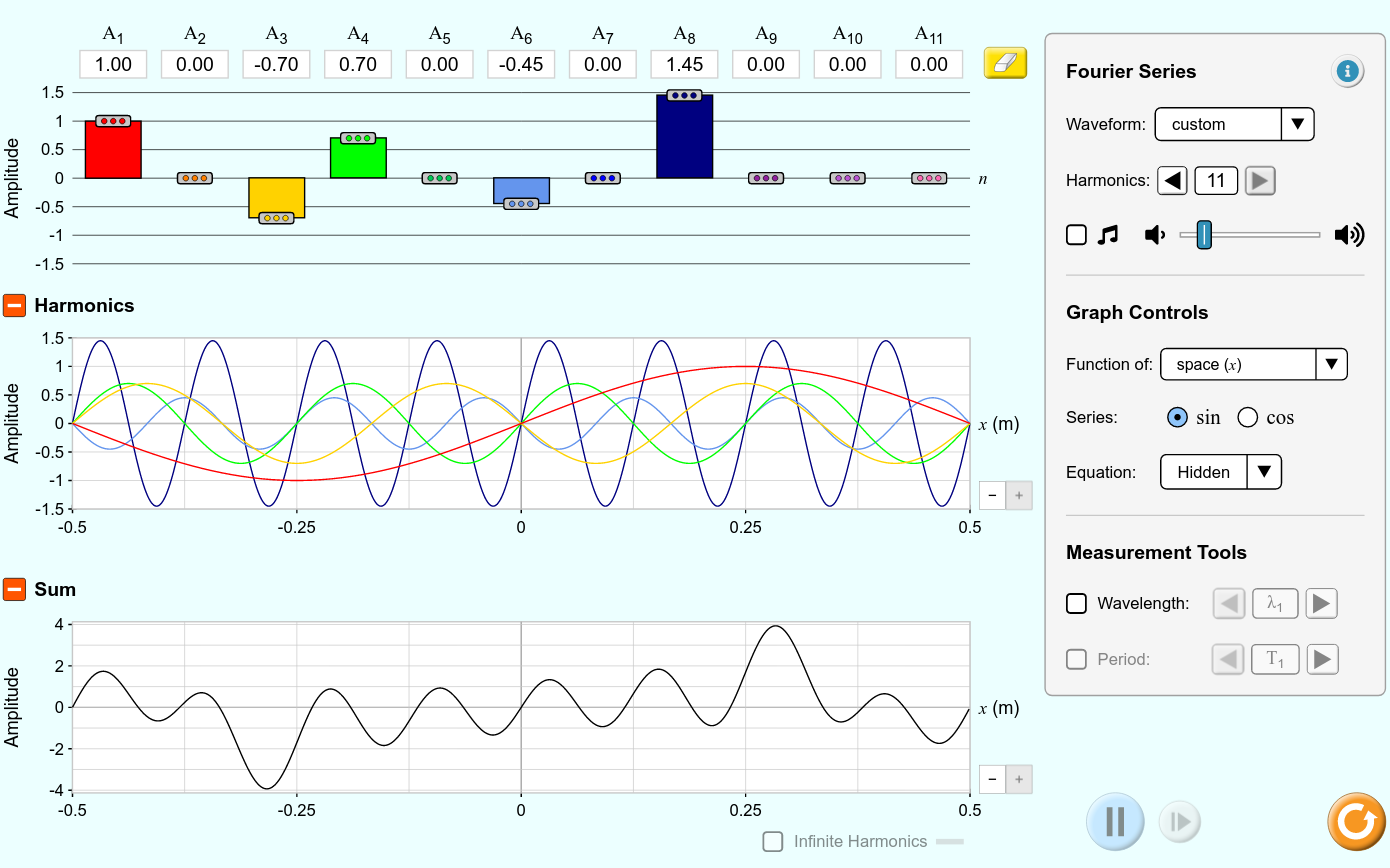
\includegraphics[width=\linewidth]{external/preview/phet-fourier-preview.png}
\end{sbspanel}%
\begin{sbspanel}{0.21}%
\noindent
\includegraphics[width=\linewidth]{generated/qrcode/interactive-phet-fourier.png}
\href{https://pretextbook.org/examples/sample-article/html/interactive-phet-fourier.html}{Standalone}%
\end{sbspanel}%
\end{sidebyside}%
\tcblower
\end{figureptx}%
Anything that suggests you can \terminology{embed} an interactive widget via an iFrame is fair game for this feature.  This is a Google Map of the state of California, for use in a French language document, from Julien Giol.  The necessary \initialism{URL} is obtained by using the ``Share'' feature, and then the ``Embed a map'' option has \initialism{HTML} with the \initialism{URL} in a \mono{@src} attribute.%
\begin{figureptx}{Figure}{California.}{map-california}{}%
\begin{sidebyside}{2}{0.075}{0.075}{0.17}%
\begin{sbspanel}{0.47}%
\noindent
\includegraphics[width=\linewidth]{generated/preview/interactive-map-california-preview.png}
\end{sbspanel}%
\begin{sbspanel}{0.21}%
\noindent
\includegraphics[width=\linewidth]{generated/qrcode/interactive-map-california.png}
\href{https://pretextbook.org/examples/sample-article/html/interactive-map-california.html}{Standalone}%
\end{sbspanel}%
\end{sidebyside}%
\tcblower
\end{figureptx}%
% end of subsection: IFrames from Servers
% end of section: Interactive Elements, Server
%
%
\typeout{************************************************}
\typeout{Section 16 Interactive Exercises}
\typeout{************************************************}
%
\section{Interactive Exercises}\label{section-interactive-exercises}%
% Introduction
Interactive components, \emph{just} for testing, no commentary.%
% end of introduction
%
%
\typeout{************************************************}
\typeout{Subsection 16.9 Faux Subsection}
\typeout{************************************************}
%
\subsection{Faux Subsection}\label{section-interactive-exercises-11}%
We used \mono{<exercises>} divisions above, and need a \mono{<subsection>} to feed the schema.%
% end of subsection: Faux Subsection
% end of section: Interactive Exercises
%
%
\typeout{************************************************}
\typeout{Section 17 Dynamic Exercises}
\typeout{************************************************}
%
\section{Dynamic Exercises}\label{section-dynamic-exercises}%
% Introduction
This section demonstrates the use of dynamic randomized exercises built upon the framework of Runestone components. These demonstration problems incorporate a library supporting mathematical expressions both for varying the content of the statement of the exercises as well as the checking of submitted answers.%
% end of introduction
% end of section: Dynamic Exercises
%
%
\typeout{************************************************}
\typeout{Section 18 Interactive Coding}
\typeout{************************************************}
%
\section{Interactive Coding}\label{section-interactive-code}%
% Introduction
More interactive components, just for testing, no commentary.%
% end of introduction
%
%
\typeout{************************************************}
\typeout{Subsection 18.4 YouTube}
\typeout{************************************************}
%
\subsection{YouTube}\label{section-interactive-code-6}%
Video, observable on a Runestone server.%
\begin{sidebyside}{2}{0.075}{0.075}{0.17}%
\begin{sbspanel}{0.47}%
\noindent
\includegraphics[width=\linewidth]{external/yt-list-variables.png}
\end{sbspanel}%
\begin{sbspanel}{0.21}%
\noindent
\includegraphics[width=\linewidth]{generated/qrcode/yt-list-vars.png}
\href{https://pretextbook.org/examples/sample-article/html/yt-list-vars.html}{Standalone}%
\end{sbspanel}%
\end{sidebyside}%
% end of subsection: YouTube
% end of section: Interactive Coding
%
%
\typeout{************************************************}
\typeout{Section 19 Audio}
\typeout{************************************************}
%
\section{Audio}\label{section-audio}%
2019-05-24: this is preliminary, and mostly based on the code for \mono{<video>} so read the next section and mimic the style from there.  But use an \mono{<audio>} element and have the \mono{@source} attribute point to an OGG, MP3, or WAV file.  Plus, an \mono{@aspect} attribute will be ignored.%
\par
We have not entirely decided how to handle the static version present in a PDF.%
\par
First in a \mono{<figure>}, so it can be cross-referenced.%
\begin{figureptx}{Figure}{MP3 Piano Trill (\mono{www.kozco.com/tech/soundtests.html})}{section-audio-5}{}%
\begin{sidebyside}{2}{0.075}{0.075}{0.17}%
\begin{sbspanel}{0.47}%
No static image provided via \mono{@preview} attribute%
\end{sbspanel}%
\begin{sbspanel}{0.21}%
\noindent
\includegraphics[width=\linewidth]{generated/qrcode/audio-piano-trill.png}
\href{https://pretextbook.org/examples/sample-article/html/audio-piano-trill.html}{Standalone}%
\end{sbspanel}%
\end{sidebyside}%
\tcblower
\end{figureptx}%
Now, naked, between a couple of paragraphs, with specified asymmetric margins, and a computed width.%
\begin{sidebyside}{2}{0.075}{0.075}{0.17}%
\begin{sbspanel}{0.47}%
No static image provided via \mono{@preview} attribute%
\end{sbspanel}%
\begin{sbspanel}{0.21}%
\noindent
\includegraphics[width=\linewidth]{generated/qrcode/audio-piano-trill-two.png}
\href{https://pretextbook.org/examples/sample-article/html/audio-piano-trill-two.html}{Standalone}%
\end{sbspanel}%
\end{sidebyside}%
\par
Now in a \mono{<sidebyside>} with an ``Organ Finale'' WAV file on the left, and on the right, Bach in OGG format at a very low bit rate (32 kps).  From \href{http://www.music.helsinki.fi/tmt/opetus/uusmedia/esim/index-e.html}{\nolinkurl{www.music.helsinki.fi/tmt/opetus/uusmedia/esim/index-e.html}}.%
\begin{sidebyside}{2}{0}{0}{0}%
\end{sidebyside}%
% end of section: Audio
%
%
\typeout{************************************************}
\typeout{Section 20 Video}
\typeout{************************************************}
%
\section{Video}\label{section-video}%
% Introduction
First, a gratuitous reference to Exercise~\hyperlink{exercises-cosine-derivative}{{\xreffont 11.2.3}} about the derivative of a cosine.%
\par
You can specify a video by a filename if you host it as part of your document, or a \initialism{URL} giving a location on the Internet.  There are a few extra features for YouTube and Vimeo videos, which are near the bottom of this page, so look there first if that meets your needs.%
% end of introduction
%
%
\typeout{************************************************}
\typeout{Subsection 20.1 Video Files}
\typeout{************************************************}
%
\subsection{Video Files}\label{section-video-3}%
Embedded videos can make sense for a web version of your document. This is a video promoting the University of Puget Sound to potential new students, in WebM format.  Support is limited to HTML5-capable browsers.  The file format can be MP4, Ogg, or WebM, though this may vary depending upon the browser.  Use a \mono{<video>} element, within either a \mono{<figure>} (numbered, captioned) or a \mono{<sidebyside>} for more precise control.   The \mono{@source} attribute in this first example \emph{does not} include an extension, and so three possibilities above will be searched for preferentially (you need only provide the video in one format, but providing additional versions will increase the chances every browser will find a compatible format).%
\begin{figureptx}{Figure}{University of Puget Sound Promotional Video}{section-video-3-3}{}%
\begin{sidebyside}{2}{0.075}{0.075}{0.17}%
\begin{sbspanel}{0.47}%
\noindent
\includegraphics[width=\linewidth]{external/preview/ups-promo-frame-one.jpg}
\end{sbspanel}%
\begin{sbspanel}{0.21}%
\noindent
\includegraphics[width=\linewidth]{generated/qrcode/ups-promo-frame-one.png}
\href{https://pretextbook.org/examples/sample-article/html/ups-promo-frame-one.html}{Standalone}%
\end{sbspanel}%
\end{sidebyside}%
\tcblower
\end{figureptx}%
You can replace the ``preview'' image of a video with one of your own making.  \initialism{HTML} refers to this as the \terminology{poster}, presumably because it advertises the video.  The image you make should be of the same quality as the video, and with the same aspect-ratio, and is presumably one of the frames of the video.  So a screenshot is the likely avenue.  (Maybe we will have advice on how to do this easily, or see \href{https://github.com/PreTeXtBook/pretext/issues/853}{Issue \#853}\footnote{\nolinkurl{github.com/PreTeXtBook/pretext/issues/853}\label{section-video-3-4-5}}.) \index{link!external, url}\index{reference!external, url} On the \mono{<video>} tag, include a \mono{@preview} attribute which is the name of an image file, including a relative path.  (JPEG or PNG formats are best.  JPEG may be smaller for video screenshots, while PNG is lossless and so may work better for diagrams.)  The next video has a preview\slash{}poster that is a fram part way into the introduction.%
\begin{figureptx}{Figure}{University of Puget Sound Promotional Video}{section-video-3-5}{}%
\begin{sidebyside}{2}{0.075}{0.075}{0.17}%
\begin{sbspanel}{0.47}%
\noindent
\includegraphics[width=\linewidth]{external/preview/ups-promo-preview.jpg}
\end{sbspanel}%
\begin{sbspanel}{0.21}%
\noindent
\includegraphics[width=\linewidth]{generated/qrcode/ups-promo-preview.png}
\href{https://pretextbook.org/examples/sample-article/html/ups-promo-preview.html}{Standalone}%
\end{sbspanel}%
\end{sidebyside}%
\tcblower
\end{figureptx}%
If you find the posters provided automatically for a video to be distracting or objectionable, you can cover them up by requesting a generic poster with the attribute-value pair: \mono{preview = \textquotedbl{}generic\textquotedbl{}}.%
\begin{figureptx}{Figure}{University of Puget Sound Promotional Video}{section-video-3-7}{}%
\begin{sidebyside}{2}{0.075}{0.075}{0.17}%
\begin{sbspanel}{0.47}%
\noindent
\includegraphics[width=\linewidth]{generated/play-button/play-button.png}
\end{sbspanel}%
\begin{sbspanel}{0.21}%
\noindent
\includegraphics[width=\linewidth]{generated/qrcode/ups-promo-generic.png}
\href{https://pretextbook.org/examples/sample-article/html/ups-promo-generic.html}{Standalone}%
\end{sbspanel}%
\end{sidebyside}%
\tcblower
\end{figureptx}%
You can use a very similar construction to point to a video hosted somewhere on the Internet, just use a complete \initialism{URL} for the \mono{<source>} attribute.  Note that if the URL has a query string (parameters following a question-mark), then any ampersands (\&) will need to be escaped, so as to not confuse the \initialism{XML} processor (i.e.\@ use \mono{\&amp}).  Also, the question-mark character needs to \emph{not} be \initialism{URL}-encoded (\mono{\%3F}), so presumably edit the \initialism{URL} to be the character.  Here are several examples, the second one uses the \mono{@start} and \mono{@stop} attributes to limit the video to just the time between the 16-second and 30-second locations, and has asymmetric margins.%
\begin{figureptx}{Figure}{Big Buck Bunny from  \href{http://camendesign.com/code/video_for_everybody/test.htm}{``Video for Everybody'' Test Page}\protect\footnotemark{}}{section-video-3-9}{}%
\begin{sidebyside}{2}{0.075}{0.075}{0.17}%
\begin{sbspanel}{0.47}%
\noindent
\includegraphics[width=\linewidth]{external/preview/big-buck-bunny-frame-one.jpg}
\end{sbspanel}%
\begin{sbspanel}{0.21}%
\noindent
\includegraphics[width=\linewidth]{generated/qrcode/big-buck-bunny-frame-one.png}
\href{https://pretextbook.org/examples/sample-article/html/big-buck-bunny-frame-one.html}{Standalone}%
\end{sbspanel}%
\end{sidebyside}%
\tcblower
\end{figureptx}%
\footnotetext[2]{\nolinkurl{camendesign.com/code/video_for_everybody/test.htm}\label{section-video-3-9-1-2}}%
\begin{figureptx}{Figure}{Big Buck Bunny, Controlled Start\slash{}End, Asymmetric Margins}{section-video-3-10}{}%
\begin{sidebyside}{2}{0.075}{0.075}{0.17}%
\begin{sbspanel}{0.47}%
\noindent
\includegraphics[width=\linewidth]{external/preview/big-buck-bunny-frame-one.jpg}
\end{sbspanel}%
\begin{sbspanel}{0.21}%
\noindent
\includegraphics[width=\linewidth]{generated/qrcode/big-buck-bunny-margins.png}
\href{https://pretextbook.org/examples/sample-article/html/big-buck-bunny-margins.html}{Standalone}%
\end{sbspanel}%
\end{sidebyside}%
\tcblower
\end{figureptx}%
\begin{figureptx}{Figure}{Big Buck Bunny, Ogg container, \mono{*.ogv} extension}{section-video-3-11}{}%
\begin{sidebyside}{2}{0.075}{0.075}{0.17}%
\begin{sbspanel}{0.47}%
\noindent
\includegraphics[width=\linewidth]{external/preview/big-buck-bunny-frame-one.jpg}
\end{sbspanel}%
\begin{sbspanel}{0.21}%
\noindent
\includegraphics[width=\linewidth]{generated/qrcode/big-buck-bunny-ogg.png}
\href{https://pretextbook.org/examples/sample-article/html/big-buck-bunny-ogg.html}{Standalone}%
\end{sbspanel}%
\end{sidebyside}%
\tcblower
\end{figureptx}%
\begin{figureptx}{Figure}{Big Buck Bunny, MP4 format}{section-video-3-12}{}%
\begin{sidebyside}{2}{0.075}{0.075}{0.17}%
\begin{sbspanel}{0.47}%
\noindent
\includegraphics[width=\linewidth]{external/preview/big-buck-bunny-frame-one.jpg}
\end{sbspanel}%
\begin{sbspanel}{0.21}%
\noindent
\includegraphics[width=\linewidth]{generated/qrcode/big-buck-bunny-mp4.png}
\href{https://pretextbook.org/examples/sample-article/html/big-buck-bunny-mp4.html}{Standalone}%
\end{sbspanel}%
\end{sidebyside}%
\tcblower
\end{figureptx}%
\begin{figureptx}{Figure}{Big Buck Bunny, WebM format}{section-video-3-13}{}%
\begin{sidebyside}{2}{0.075}{0.075}{0.17}%
\begin{sbspanel}{0.47}%
\noindent
\includegraphics[width=\linewidth]{external/preview/big-buck-bunny-frame-one.jpg}
\end{sbspanel}%
\begin{sbspanel}{0.21}%
\noindent
\includegraphics[width=\linewidth]{generated/qrcode/big-buck-bunny-webm.png}
\href{https://pretextbook.org/examples/sample-article/html/big-buck-bunny-webm.html}{Standalone}%
\end{sbspanel}%
\end{sidebyside}%
\tcblower
\end{figureptx}%
\begin{figureptx}{Figure}{Big Buck Bunny, Automatic best format (temporarily broken)}{section-video-3-14}{}%
\begin{sidebyside}{2}{0.075}{0.075}{0.17}%
\begin{sbspanel}{0.47}%
\noindent
\includegraphics[width=\linewidth]{external/preview/big-buck-bunny-frame-one.jpg}
\end{sbspanel}%
\begin{sbspanel}{0.21}%
\noindent
\includegraphics[width=\linewidth]{generated/qrcode/big-buck-bunny-best-format.png}
\href{https://pretextbook.org/examples/sample-article/html/big-buck-bunny-best-format.html}{Standalone}%
\end{sbspanel}%
\end{sidebyside}%
\tcblower
\end{figureptx}%
Videos are assumed to have a 16:9 aspect ratio (width:height).  If this is not the case, then you must specify the aspect ratio with either a ratio (e.g. 4:3) or as a number expressing the fraction width\slash{}height (e.g. 1.3333).  Four decimal places should suffice for the latter.  Note that you cannot \emph{change} the aspect ratio, and you \emph{must} supply the aspect ratio for any video that does not have the default ratio.  This is a technical requirement that allows us to smoothly scale the videos on small devices (try this page on your mobile phone!).%
% end of subsection: Video Files
%
%
\typeout{************************************************}
\typeout{Subsection 20.2 YouTube}
\typeout{************************************************}
%
\subsection{YouTube}\label{section-video-4}%
YouTube\index{YouTube videos}\index{videos!YouTube} videos may be embedded with only knowledge of a video's ``ID'' or a ``playlist ID''.  A single video's YouTube ID is a string of eleven seemingly random characters that show up in the URL when you watch a video.  For the Led Zeppelin performance below, the ID is \mono{hAzdgU\_kpGo}, which you might normally watch directly from the URL \href{https://www.youtube.com/watch?v=hAzdgU_kpGo}{\nolinkurl{www.youtube.com/watch?v=hAzdgU_kpGo}}.  As described just above, you need to specify a different aspect ratio if the video does not have a 16:9 aspect ratio.%
\par
Note: some of these videos may not play if viewed locally, and maybe not even if you start up a local web server (such as can be easily done with Python).  So if you are testing new features, be careful about assuming videos from cloud services are not working properly.%
\par
If you have ever owned a drone, you sympathize with this guy.  Way funnier than a cat video.%
\begin{figureptx}{Figure}{First Drone Flight (1:28)}{section-video-4-5}{}%
\begin{sidebyside}{2}{0.075}{0.075}{0.17}%
\begin{sbspanel}{0.47}%
\noindent
\includegraphics[width=\linewidth]{generated/youtube/drone-flight-full.jpg}
\end{sbspanel}%
\begin{sbspanel}{0.21}%
\noindent
\includegraphics[width=\linewidth]{generated/qrcode/drone-flight-full.png}
\href{https://pretextbook.org/examples/sample-article/html/drone-flight-full.html}{Standalone}%
\end{sbspanel}%
\end{sidebyside}%
\tcblower
\end{figureptx}%
If you are only interested in a piece of the action, you can limit the video with \mono{start} and \mono{end} attributes in seconds.  You might make those times clear in the caption for readers getting the link out of a PDF.  Some videos may not respect these parameters.%
\begin{figureptx}{Figure}{First Drone Flight (Splashdown, 0:54 to 1:12)}{section-video-4-7}{}%
\begin{sidebyside}{2}{0.075}{0.075}{0.17}%
\begin{sbspanel}{0.47}%
\noindent
\includegraphics[width=\linewidth]{generated/youtube/drone-flight-clip.jpg}
\end{sbspanel}%
\begin{sbspanel}{0.21}%
\noindent
\includegraphics[width=\linewidth]{generated/qrcode/drone-flight-clip.png}
\href{https://pretextbook.org/examples/sample-article/html/drone-flight-clip.html}{Standalone}%
\end{sbspanel}%
\end{sidebyside}%
\tcblower
\end{figureptx}%
This next video comes with a default poster from YouTube featuring Robert Plant.  We've replaced it with a poster featuring Jimmy Page.%
\begin{figureptx}{Figure}{Kashmir (Live), Led Zeppelin. O2 Arena, London. December 10, 2007. (8:55)}{section-video-4-9}{}%
\index{Led Zeppelin video}%
\begin{sidebyside}{2}{0.075}{0.075}{0.17}%
\begin{sbspanel}{0.47}%
\noindent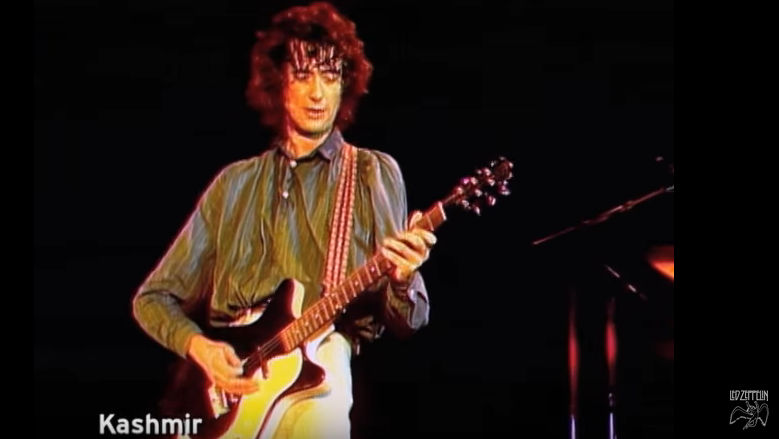
\includegraphics[width=\linewidth]{external/preview/jimmy-page.jpg}
\end{sbspanel}%
\begin{sbspanel}{0.21}%
\noindent
\includegraphics[width=\linewidth]{generated/qrcode/led-zeppelin-kashmir.png}
\href{https://pretextbook.org/examples/sample-article/html/led-zeppelin-kashmir.html}{Standalone}%
\end{sbspanel}%
\end{sidebyside}%
\tcblower
\end{figureptx}%
And if you don't want to be reminded of Plant, Page, Bonham, or Jones, you can cover them up entirely.%
\begin{figureptx}{Figure}{Kashmir (Live), Led Zeppelin. O2 Arena, London. December 10, 2007. (8:55)}{section-video-4-11}{}%
\index{Led Zeppelin video}%
\begin{sidebyside}{2}{0.075}{0.075}{0.17}%
\begin{sbspanel}{0.47}%
\noindent
\includegraphics[width=\linewidth]{generated/play-button/play-button.png}
\end{sbspanel}%
\begin{sbspanel}{0.21}%
\noindent
\includegraphics[width=\linewidth]{generated/qrcode/led-zeppelin-kashmir-generic.png}
\href{https://pretextbook.org/examples/sample-article/html/led-zeppelin-kashmir-generic.html}{Standalone}%
\end{sbspanel}%
\end{sidebyside}%
\tcblower
\end{figureptx}%
Videos were first designed mostly on the assumption that they are wrapped in a \mono{figure} with a \mono{title} (which is distinct from a \mono{caption}).  But you can just place a video ``naked'' inbetween a couple of paragraphs.  This is nice if you don't want the clutter of numbers, and\slash{}or if you plan to exclude videos from some edition of your document.%
\begin{sidebyside}{2}{0.075}{0.075}{0.17}%
\begin{sbspanel}{0.47}%
\noindent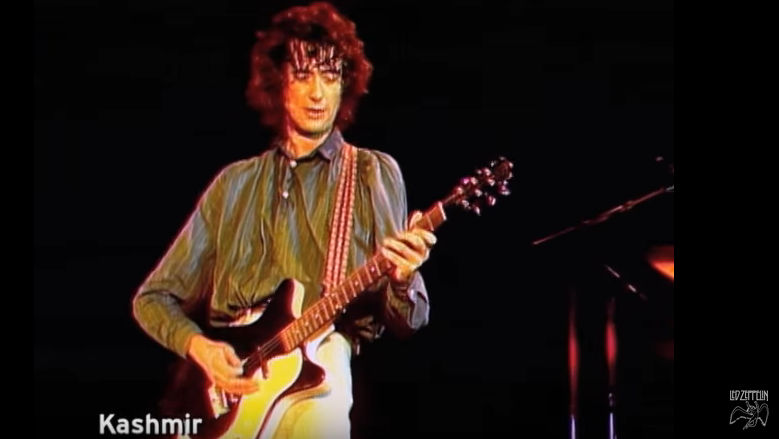
\includegraphics[width=\linewidth]{external/preview/jimmy-page.jpg}
\end{sbspanel}%
\begin{sbspanel}{0.21}%
\noindent
\includegraphics[width=\linewidth]{generated/qrcode/led-zeppelin-kashmir-solo.png}
\href{https://pretextbook.org/examples/sample-article/html/led-zeppelin-kashmir-solo.html}{Standalone}%
\end{sbspanel}%
\end{sidebyside}%
\par
We can pack two videos side-by-side, with a lot of horizontal control, using two panels in the \mono{sidebyside} element.  We have simply chosen here to not provide a caption (overall, or separately) as an illustration.  The sizes are purposely a bit odd.  See \hyperref[section-side-by-side]{Section~{\xreffont\ref{section-side-by-side}}} for much more on side-by-side panels.  These videos come from the ``Topic'' and ``VEVO'' areas of YouTube (respectively) and both have start\slash{}end times.%
\begin{sidebyside}{2}{0.1}{0.1}{0.2}%
\end{sidebyside}%
\par
These next two videos are evenly spaced, one from YouTube, one from a source file hosted by the author.  Now with separate captions, but identical margins (through very different choices of layout parameters than in the preceding pair of videos).%
\begin{sidebyside}{2}{0.1}{0.1}{0.1}%
\begin{sbspanel}{0.35}%
\begin{panelfigureptx}{Figure}{Drone Flight}{section-video-4-17-1}{}%
\begin{sidebyside}{2}{0.075}{0.075}{0.17}%
\begin{sbspanel}{0.47}%
\noindent
\includegraphics[width=\linewidth]{generated/youtube/drone-flight-sbs.jpg}
\end{sbspanel}%
\begin{sbspanel}{0.21}%
\noindent
\includegraphics[width=\linewidth]{generated/qrcode/drone-flight-sbs.png}
\href{https://pretextbook.org/examples/sample-article/html/drone-flight-sbs.html}{Standalone}%
\end{sbspanel}%
\end{sidebyside}%
\tcblower
\end{panelfigureptx}%
\end{sbspanel}%
\begin{sbspanel}{0.35}%
\begin{panelfigureptx}{Figure}{UPS Promo}{section-video-4-17-2}{}%
\begin{sidebyside}{2}{0.075}{0.075}{0.17}%
\begin{sbspanel}{0.47}%
\noindent
\includegraphics[width=\linewidth]{external/preview/ups-promo-frame-one.jpg}
\end{sbspanel}%
\begin{sbspanel}{0.21}%
\noindent
\includegraphics[width=\linewidth]{generated/qrcode/ups-promo-sbs.png}
\href{https://pretextbook.org/examples/sample-article/html/ups-promo-sbs.html}{Standalone}%
\end{sbspanel}%
\end{sidebyside}%
\tcblower
\end{panelfigureptx}%
\end{sbspanel}%
\end{sidebyside}%
\par
A YouTube ``playlist'' can be built in one of two ways. You may specify the \mono{youtube} attribute to be a space-separated list of several video IDs. Alternatively, you may set the \mono{youtubeplaylist} attribute to a YouTube playlist ID.%
\begin{sidebyside}{2}{0}{0}{0.06}%
\begin{sbspanel}{0.47}%
\begin{panelfigureptx}{Figure}{Individual IDs specified in an ``itemized'' playlist}{section-video-4-19-1}{}%
\begin{sidebyside}{2}{0.075}{0.075}{0.17}%
\begin{sbspanel}{0.47}%
\noindent
\includegraphics[width=\linewidth]{generated/youtube/zeppelin-playlist.jpg}
\end{sbspanel}%
\begin{sbspanel}{0.21}%
\noindent
\includegraphics[width=\linewidth]{generated/qrcode/zeppelin-playlist.png}
\href{https://pretextbook.org/examples/sample-article/html/zeppelin-playlist.html}{Standalone}%
\end{sbspanel}%
\end{sidebyside}%
\tcblower
\end{panelfigureptx}%
\end{sbspanel}%
\begin{sbspanel}{0.47}%
\begin{panelfigureptx}{Figure}{YouTube playlist ID specified in a ``named'' playlist}{section-video-4-19-2}{}%
\begin{sidebyside}{2}{0.075}{0.075}{0.17}%
\begin{sbspanel}{0.47}%
\noindent
\includegraphics[width=\linewidth]{generated/play-button/play-button.png}
\end{sbspanel}%
\begin{sbspanel}{0.21}%
\noindent
\includegraphics[width=\linewidth]{generated/qrcode/zeppelin-playlist-named.png}
\href{https://pretextbook.org/examples/sample-article/html/zeppelin-playlist-named.html}{Standalone}%
\end{sbspanel}%
\end{sidebyside}%
\tcblower
\end{panelfigureptx}%
\end{sbspanel}%
\end{sidebyside}%
\par
We test three equally-wide YouTube videos in a \mono{<sidebyside>} with a few variations.%
\begin{sidebyside}{3}{0}{0}{0.05}%
\begin{sbspanel}{0.3}%
\begin{panelfigureptx}{Figure}{Medium Length}{section-video-4-21-1}{}%
\begin{sidebyside}{2}{0.075}{0.075}{0.17}%
\begin{sbspanel}{0.47}%
\noindent
\includegraphics[width=\linewidth]{generated/youtube/pre-roll-countdown-1.jpg}
\end{sbspanel}%
\begin{sbspanel}{0.21}%
\noindent
\includegraphics[width=\linewidth]{generated/qrcode/pre-roll-countdown-1.png}
\href{https://pretextbook.org/examples/sample-article/html/pre-roll-countdown-1.html}{Standalone}%
\end{sbspanel}%
\end{sidebyside}%
\tcblower
\end{panelfigureptx}%
\end{sbspanel}%
\begin{sbspanel}{0.3}%
\begin{panelfigureptx}{Figure}{Short}{section-video-4-21-2}{}%
\begin{sidebyside}{2}{0.075}{0.075}{0.17}%
\begin{sbspanel}{0.47}%
\noindent
\includegraphics[width=\linewidth]{generated/youtube/pre-roll-countdown-2.jpg}
\end{sbspanel}%
\begin{sbspanel}{0.21}%
\noindent
\includegraphics[width=\linewidth]{generated/qrcode/pre-roll-countdown-2.png}
\href{https://pretextbook.org/examples/sample-article/html/pre-roll-countdown-2.html}{Standalone}%
\end{sbspanel}%
\end{sidebyside}%
\tcblower
\end{panelfigureptx}%
\end{sbspanel}%
\begin{sbspanel}{0.3}%
\begin{panelfigureptx}{Figure}{A Really Long Caption That Will Wrap onto a New Line}{section-video-4-21-3}{}%
\begin{sidebyside}{2}{0.075}{0.075}{0.17}%
\begin{sbspanel}{0.47}%
\noindent
\includegraphics[width=\linewidth]{generated/youtube/pre-roll-countdown-3.jpg}
\end{sbspanel}%
\begin{sbspanel}{0.21}%
\noindent
\includegraphics[width=\linewidth]{generated/qrcode/pre-roll-countdown-3.png}
\href{https://pretextbook.org/examples/sample-article/html/pre-roll-countdown-3.html}{Standalone}%
\end{sbspanel}%
\end{sidebyside}%
\tcblower
\end{panelfigureptx}%
\end{sbspanel}%
\end{sidebyside}%
\par
We test three equally-wide YouTube videos in a \mono{<sidebyside>} with a few variations, and now contained in a \mono{<figure>}.%
\begin{figureptx}{Figure}{Author-Hosted videos as Sub-Figures}{section-video-4-23}{}%
\begin{sidebyside}{3}{0}{0}{0.05}%
\begin{sbspanel}{0.3}%
\begin{subfigureptx}{Figure}{Medium Length}{section-video-4-23-2-1}{}%
\begin{sidebyside}{2}{0.075}{0.075}{0.17}%
\begin{sbspanel}{0.47}%
\noindent
\includegraphics[width=\linewidth]{generated/youtube/pre-roll-countdown-4.jpg}
\end{sbspanel}%
\begin{sbspanel}{0.21}%
\noindent
\includegraphics[width=\linewidth]{generated/qrcode/pre-roll-countdown-4.png}
\href{https://pretextbook.org/examples/sample-article/html/pre-roll-countdown-4.html}{Standalone}%
\end{sbspanel}%
\end{sidebyside}%
\tcblower
\end{subfigureptx}%
\end{sbspanel}%
\begin{sbspanel}{0.3}%
\begin{subfigureptx}{Figure}{Short}{section-video-4-23-2-2}{}%
\begin{sidebyside}{2}{0.075}{0.075}{0.17}%
\begin{sbspanel}{0.47}%
\noindent
\includegraphics[width=\linewidth]{generated/youtube/pre-roll-countdown-5.jpg}
\end{sbspanel}%
\begin{sbspanel}{0.21}%
\noindent
\includegraphics[width=\linewidth]{generated/qrcode/pre-roll-countdown-5.png}
\href{https://pretextbook.org/examples/sample-article/html/pre-roll-countdown-5.html}{Standalone}%
\end{sbspanel}%
\end{sidebyside}%
\tcblower
\end{subfigureptx}%
\end{sbspanel}%
\begin{sbspanel}{0.3}%
\begin{subfigureptx}{Figure}{A Really Long Caption That Will Wrap onto a New Line}{section-video-4-23-2-3}{}%
\begin{sidebyside}{2}{0.075}{0.075}{0.17}%
\begin{sbspanel}{0.47}%
\noindent
\includegraphics[width=\linewidth]{generated/youtube/pre-roll-countdown-6.jpg}
\end{sbspanel}%
\begin{sbspanel}{0.21}%
\noindent
\includegraphics[width=\linewidth]{generated/qrcode/pre-roll-countdown-6.png}
\href{https://pretextbook.org/examples/sample-article/html/pre-roll-countdown-6.html}{Standalone}%
\end{sbspanel}%
\end{sidebyside}%
\tcblower
\end{subfigureptx}%
\end{sbspanel}%
\end{sidebyside}%
\tcblower
\end{figureptx}%
We test three equally-wide author-hosted videos in a \mono{<sidebyside>} with a few variations.%
\begin{sidebyside}{3}{0}{0}{0.05}%
\begin{sbspanel}{0.3}%
\begin{panelfigureptx}{Figure}{Medium Length}{section-video-4-25-1}{}%
\begin{sidebyside}{2}{0.075}{0.075}{0.17}%
\begin{sbspanel}{0.47}%
\noindent
\includegraphics[width=\linewidth]{external/preview/ups-promo-preview.jpg}
\end{sbspanel}%
\begin{sbspanel}{0.21}%
\noindent
\includegraphics[width=\linewidth]{generated/qrcode/ups-promo-1.png}
\href{https://pretextbook.org/examples/sample-article/html/ups-promo-1.html}{Standalone}%
\end{sbspanel}%
\end{sidebyside}%
\tcblower
\end{panelfigureptx}%
\end{sbspanel}%
\begin{sbspanel}{0.3}%
\begin{panelfigureptx}{Figure}{Short}{section-video-4-25-2}{}%
\begin{sidebyside}{2}{0.075}{0.075}{0.17}%
\begin{sbspanel}{0.47}%
\noindent
\includegraphics[width=\linewidth]{external/preview/ups-promo-preview.jpg}
\end{sbspanel}%
\begin{sbspanel}{0.21}%
\noindent
\includegraphics[width=\linewidth]{generated/qrcode/ups-promo-2.png}
\href{https://pretextbook.org/examples/sample-article/html/ups-promo-2.html}{Standalone}%
\end{sbspanel}%
\end{sidebyside}%
\tcblower
\end{panelfigureptx}%
\end{sbspanel}%
\begin{sbspanel}{0.3}%
\begin{panelfigureptx}{Figure}{A Really Long Caption That Will Wrap onto a New Line}{section-video-4-25-3}{}%
\begin{sidebyside}{2}{0.075}{0.075}{0.17}%
\begin{sbspanel}{0.47}%
\noindent
\includegraphics[width=\linewidth]{external/preview/ups-promo-preview.jpg}
\end{sbspanel}%
\begin{sbspanel}{0.21}%
\noindent
\includegraphics[width=\linewidth]{generated/qrcode/ups-promo-3.png}
\href{https://pretextbook.org/examples/sample-article/html/ups-promo-3.html}{Standalone}%
\end{sbspanel}%
\end{sidebyside}%
\tcblower
\end{panelfigureptx}%
\end{sbspanel}%
\end{sidebyside}%
\par
We test three equally-wide author-hosted videos in a \mono{<sidebyside>} with a few variations, and now contained in a \mono{<figure>}.%
\begin{figureptx}{Figure}{YouTube videos as Sub-Figures}{section-video-4-27}{}%
\begin{sidebyside}{3}{0}{0}{0.05}%
\begin{sbspanel}{0.3}%
\begin{subfigureptx}{Figure}{Medium Length}{section-video-4-27-2-1}{}%
\begin{sidebyside}{2}{0.075}{0.075}{0.17}%
\begin{sbspanel}{0.47}%
\noindent
\includegraphics[width=\linewidth]{external/preview/ups-promo-preview.jpg}
\end{sbspanel}%
\begin{sbspanel}{0.21}%
\noindent
\includegraphics[width=\linewidth]{generated/qrcode/ups-promo-4.png}
\href{https://pretextbook.org/examples/sample-article/html/ups-promo-4.html}{Standalone}%
\end{sbspanel}%
\end{sidebyside}%
\tcblower
\end{subfigureptx}%
\end{sbspanel}%
\begin{sbspanel}{0.3}%
\begin{subfigureptx}{Figure}{Short}{section-video-4-27-2-2}{}%
\begin{sidebyside}{2}{0.075}{0.075}{0.17}%
\begin{sbspanel}{0.47}%
\noindent
\includegraphics[width=\linewidth]{external/preview/ups-promo-preview.jpg}
\end{sbspanel}%
\begin{sbspanel}{0.21}%
\noindent
\includegraphics[width=\linewidth]{generated/qrcode/ups-promo-5.png}
\href{https://pretextbook.org/examples/sample-article/html/ups-promo-5.html}{Standalone}%
\end{sbspanel}%
\end{sidebyside}%
\tcblower
\end{subfigureptx}%
\end{sbspanel}%
\begin{sbspanel}{0.3}%
\begin{subfigureptx}{Figure}{A Really Long Caption That Will Wrap onto a New Line}{section-video-4-27-2-3}{}%
\begin{sidebyside}{2}{0.075}{0.075}{0.17}%
\begin{sbspanel}{0.47}%
\noindent
\includegraphics[width=\linewidth]{external/preview/ups-promo-preview.jpg}
\end{sbspanel}%
\begin{sbspanel}{0.21}%
\noindent
\includegraphics[width=\linewidth]{generated/qrcode/ups-promo-6.png}
\href{https://pretextbook.org/examples/sample-article/html/ups-promo-6.html}{Standalone}%
\end{sbspanel}%
\end{sidebyside}%
\tcblower
\end{subfigureptx}%
\end{sbspanel}%
\end{sidebyside}%
\tcblower
\end{figureptx}%
% end of subsection: YouTube
%
%
\typeout{************************************************}
\typeout{Subsection 20.3 Vimeo}
\typeout{************************************************}
%
\subsection{Vimeo}\label{section-video-5}%
We support videos from \href{https://vimeo.com/}{Vimeo}\footnote{\nolinkurl{vimeo.com}\label{section-video-5-2-2}} in much the same way as YouTube videos.  Now the identifier is a long integer.  For example, the video up next would normally be found at \mono{https://vimeo.com/27246366}.  But instead, you can embed the video with as little as \mono{<video vimeo=\textquotedbl{}27246366\textquotedbl{}/>}.  As of 2019-05-18, we intend to support as many of the options described above as possible.  Widths and heights (via the aspect ratio) will perform as expected.  We have not investigated start and end times.%
\begin{figureptx}{Figure}{``MOVE'', by \href{https://vimeo.com/rickmereki}{Rick Mereki}\protect\footnotemark{}, \mono{vimeo.com/rickmereki}}{section-video-5-3}{}%
\begin{sidebyside}{2}{0.075}{0.075}{0.17}%
\begin{sbspanel}{0.47}%
\noindent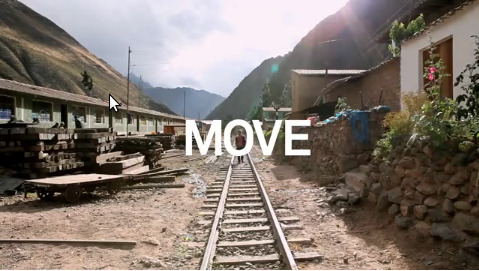
\includegraphics[width=\linewidth]{external/preview/vimeo-move.jpg}
\end{sbspanel}%
\begin{sbspanel}{0.21}%
\noindent
\includegraphics[width=\linewidth]{generated/qrcode/vimeo-move.png}
\href{https://pretextbook.org/examples/sample-article/html/vimeo-move.html}{Standalone}%
\end{sbspanel}%
\end{sidebyside}%
\tcblower
\end{figureptx}%
\footnotetext[4]{\nolinkurl{vimeo.com/rickmereki}\label{section-video-5-3-1-3}}%
Now with an author-supplied poster.%
\begin{figureptx}{Figure}{``MOVE'', by \href{https://vimeo.com/rickmereki}{Rick Mereki}\protect\footnotemark{}, \mono{vimeo.com/rickmereki}}{section-video-5-5}{}%
\begin{sidebyside}{2}{0.075}{0.075}{0.17}%
\begin{sbspanel}{0.47}%
\noindent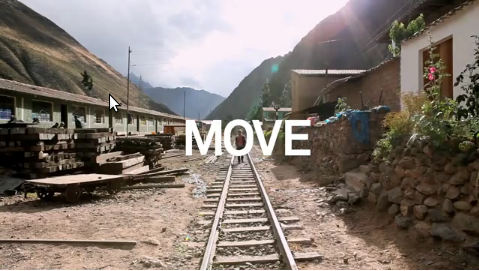
\includegraphics[width=\linewidth]{external/preview/move.png}
\end{sbspanel}%
\begin{sbspanel}{0.21}%
\noindent
\includegraphics[width=\linewidth]{generated/qrcode/section-video-5-5-2.png}
\href{https://pretextbook.org/examples/sample-article/html/section-video-5-5-2.html}{Standalone}%
\end{sbspanel}%
\end{sidebyside}%
\tcblower
\end{figureptx}%
\footnotetext[5]{\nolinkurl{vimeo.com/rickmereki}\label{section-video-5-5-1-3}}%
% end of subsection: Vimeo
%
%
\typeout{************************************************}
\typeout{Subsection 20.4 Captions and Subtitles}
\typeout{************************************************}
%
\subsection{Captions and Subtitles}\label{section-video-6}%
Experimental support for captions and subtitles first.  Look at the source, which mimics the actual HTML.  The words of the titles and\slash{}or subcaptions (there is a difference!) come from a file in \href{https://en.wikipedia.org/wiki/WebVTT}{Web Video Text Tracks}\footnote{\nolinkurl{wikipedia.org/wiki/WebVTT}\label{section-video-6-2-2}} (\initialism{WEBVVT}) format.%
\begin{figureptx}{Figure}{Big Buck Bunny with subtitles adapted from \href{https://sites.google.com/site/chrisfoo/subtitles}{\nolinkurl{https://sites.google.com/site/chrisfoo/subtitles}}}{section-video-6-3}{}%
\begin{sidebyside}{2}{0.075}{0.075}{0.17}%
\begin{sbspanel}{0.47}%
\noindent
\includegraphics[width=\linewidth]{external/preview/big-buck-bunny-frame-one.jpg}
\end{sbspanel}%
\begin{sbspanel}{0.21}%
\noindent
\includegraphics[width=\linewidth]{generated/qrcode/big-buck-bunny-subtitles.png}
\href{https://pretextbook.org/examples/sample-article/html/big-buck-bunny-subtitles.html}{Standalone}%
\end{sbspanel}%
\end{sidebyside}%
\tcblower
\end{figureptx}%
This video is identical to the previous one, except it tests the use of a default \mono{<track>}.  The \mono{@default} attribute on \mono{<track>} can be set to the value \mono{yes} to make one set of captions the default (and only one!).  Test is a bit lame, the two \mono{<track>} use the same file, but just have different labels for the player's menu.  Track named \mono{US English Two} will show as in-use at start-up.%
\begin{sidebyside}{2}{0.075}{0.075}{0.17}%
\begin{sbspanel}{0.47}%
\noindent
\includegraphics[width=\linewidth]{external/preview/big-buck-bunny-frame-one.jpg}
\end{sbspanel}%
\begin{sbspanel}{0.21}%
\noindent
\includegraphics[width=\linewidth]{generated/qrcode/big-buck-bunny-two-subtitles.png}
\href{https://pretextbook.org/examples/sample-article/html/big-buck-bunny-two-subtitles.html}{Standalone}%
\end{sbspanel}%
\end{sidebyside}%
% end of subsection: Captions and Subtitles
% end of section: Video
%
%
\typeout{************************************************}
\typeout{Section 21 Cross-Referencing}
\typeout{************************************************}
%
\section{Cross-Referencing}\label{section-cross-referencing}%
Cross-references\index{cross-reference} are easy, since that is a key reason for having a highly structured document.  Here is a useful feature if you elect to use it.  Any \mono{<xref>} will ``know'' what it points to, so you can let it provide the ``naming'' part of the cross-reference text.  You can turn this on globally with the command-line parameter \mono{autoname}\index{autoname} set to \mono{\textquotesingle{}yes\textquotesingle{}}.  If you do that, you will see most of the names in this document doubled, since the names are written into the source already in most places outside of this section.%
\par
Moreover, the names themselves will change with the use of the one language dependent file.  And another bonus is that with an autoname, you automatically get a \emph{non-breaking} space between the name and the reference.  The autoname switch makes no sense for ``provisional'' cross-references, since there is no information about what they point to.%
\par
Here is a reference that has no indication of its type in the source:  \hyperref[theorem-FTC]{{\xreffont\ref{theorem-FTC}}}.  So by default you will just see a number that you can click on.  If you use the \mono{text=\textquotedbl{}type-global\textquotedbl{}} switch then you should see ``Theorem'' prepended.  Note that if you changed the theorem to a lemma, then that change would be reflected here automatically when autonaming is in effect.%
\par
If you set the autonaming behavior globally, or accept the default behavior, there will still be instances where you want to override that choice.  Simple: just say \mono{text=\textquotedbl{}type-global\textquotedbl{}} or \mono{text=\textquotedbl{}global\textquotedbl{}} as part of the \mono{xref}.  Each example below should look the same each time this article is processed, no matter how the global \mono{autoname} is set.%
\begin{itemize}[label=\textbullet]
\item{}No name ever: \hyperref[corollary-FTC-derivative]{{\xreffont\ref{corollary-FTC-derivative}}}%
\item{}Always named: \hyperref[corollary-FTC-derivative]{Corollary~{\xreffont\ref{corollary-FTC-derivative}}}%
\end{itemize}
%
\par
You might also wish to provide a prefix to a cross-reference and have it incorporated into the text of what you would click on in an electronic version.  So if you make an \mono{xref} with some content, then that content will prefix the cross-reference within the clickable\slash{}pokeable text and be attached with a non-breaking space.  This \mono{xref} content totally overrides any prefix that might happen otherwise.  So the name of an item (e.g.\@ ``corollary'') could be replaced, and if you make a cross-reference with custom text, that will be the clickable also.  An example:%
\begin{itemize}[label=\textbullet]
\item{}A grand result: \hyperref[corollary-FTC-derivative]{Major Corollary~{\xreffont\ref{corollary-FTC-derivative}}}%
\item{}A grand result: \hyperref[corollary-FTC-derivative]{a nice corollary}%
\end{itemize}
%
\par
Suppose you want to reference two theorems, so you might want to say something like ``Theorems 4.6 and 5.2.''  With global autonaming on, you can override the first \mono{Theorem} by providing the content \mono{Theorems} on the first \mono{xref} and \mono{text=\textquotedbl{}global\textquotedbl{}} on the second \mono{xref}.  (With global autonaming off, you will also get what you want\slash{}expect.)   Here is the test, which should look correct no matter what the global switch is:  \hyperref[section-cross-referencing]{Sections~{\xreffont\ref{section-cross-referencing}}} and \hyperref[section-internationalization]{{\xreffont\ref{section-internationalization}}}.  (But notice that it is up to you to be certain the types of these targets do not change without you changing the content of the first \mono{xref}.  The ``author-tools'' mode and careful choices of \mono{xml:id} strings can help avoid this trap.)%
\par
If you set the value of \mono{@text} to \mono{title}, then the title you assigned to the theorem will be used as the link for a cross-reference.  Here is a the final example, which refers to a fundamental theorem by name \hyperref[theorem-FTC]{The Fundamental Theorem of Calculus}.%
\par
Cross-references to exercises with hard-coded numbers should respect the supplied number.  Exercise~\hyperlink{exercise-with-hardcoded-number}{{\xreffont 39.42a}} should reference problem 42a.%
\par
Here we form a list to test pointing at various structures.  Each of the following should open a knowl in the HTML version, otherwise it will be a traditional hyperlink (if possible).  Note that if a knowl opens, there will always be an ``in-context'' link which will take you to the actual location, should you have  wished instead to just go there.%
\begin{itemize}[label=\textbullet]
\item{}Footnotes: Fermat allusion at \hyperref[footnote-fermat]{{\xreffont 2.1}}.%
\item{}Citations: Judson's AATA with annotation at \hyperlink{biblio-judson-AATA}{[{\xreffont 1}]}%
\item{}Citations: Judson's AATA with autoname that should have zero effect \hyperlink{biblio-judson-AATA}{[{\xreffont 1}]}%
\item{}Citations: In a \mono{<references>} division inside an appendix \hyperlink{biblio-strang-article-uno}{[{\xreffont J.2.1}]}%
\item{}Note: just the annotation of previous citation at \hyperlink{note-judson-AATA}{{\xreffont 1.1}}%
\item{}Examples: Mystery derivative at \hyperref[example-mysterious]{{\xreffont\ref{example-mysterious}}}, or a question at \hyperref[sample-question]{{\xreffont\ref{sample-question}}}.%
\item{}Definition-like: A mathematical statement with no proof \hyperref[principle-principle]{{\xreffont\ref{principle-principle}}}.%
\item{}A numbered Note: \hyperref[note-remark]{{\xreffont\ref{note-remark}}}%
\item{}A link to a \mono{proposition} element, while this document has globally renamed \mono{proposition}s as ``Conundrum''s, so this link should use the new name: \hyperref[proposition-as-conundrum]{Conundrum~{\xreffont\ref{proposition-as-conundrum}}}%
\item{}Theorems: Fundamental Theorem of Calculus, with proof at \hyperref[theorem-FTC]{{\xreffont\ref{theorem-FTC}}}%
\item{}Proof: of second version of FTC at \hyperlink{proof-FTC-corollary}{{\xreffont 4.1.1}}%
\item{}Figures: A plot with a derivative at \hyperref[figure-function-derivative]{{\xreffont\ref{figure-function-derivative}}}.%
\item{}A Figure within a side-by-side panel, with its own number: \hyperref[another-regular-figure]{{\xreffont\ref{another-regular-figure}}}%
\item{}A Table within a side-by-side panel, with a subnumber: \hyperref[table-sidebyside-subtable]{{\xreffont\ref{table-sidebyside-subtable}}}%
\item{}A Figure, containing a side-by-side with two sub-captioned images: \hyperref[fig-sidebyside-global]{{\xreffont\ref{fig-sidebyside-global}}}%
\item{}Display Mathematics: single, first with no name: \hyperref[equation-alternate-FTC]{({\xreffont\ref{equation-alternate-FTC}})}.  Then with an autoname: \hyperref[equation-alternate-FTC]{({\xreffont\ref{equation-alternate-FTC}})}.%
\item{}Display Mathematics: multi-row, first with no name: \hyperref[equation-use-FTC]{({\xreffont\ref{equation-use-FTC}})}.  Then with an autoname: \hyperref[equation-use-FTC]{({\xreffont\ref{equation-use-FTC}})}.  And two, with a plural form: \hyperref[equation-alternate-FTC]{Equations~({\xreffont\ref{equation-alternate-FTC}})} and \hyperref[equation-use-FTC]{({\xreffont\ref{equation-use-FTC}})}.%
\item{}You can cross-reference \hyperref[equation-use-FTC]{The Fundamental Theorem of Calculus} via custom text of your choice.%
\item{}Display mathematics: an equation with  ``local'' tag, which should not be used so very far away: \hyperref[equation-local-star]{({\xreffont\ref{equation-local-star}})}.%
\item{}You can author a cross-reference to a displayed equation with no number, but it will not be very satisfying.  You should get a warning if you try.%
\item{}Exercises (divisional), a range, with plural form provided to override autonaming: \hyperlink{exercises-null-problem}{Exercises~{\xreffont 11.2.1}\textendash{}{\xreffont 11.2.3}}.%
\item{}Exercise (inline): with enclosed hint at \hyperref[exercise-essay]{{\xreffont\ref{exercise-essay}}}%
\item{}A group of two exercises, with introduction, conclusion: \hyperlink{exercisegroup-two-problems}{Exercise Group~{\xreffont 11.2.2\textendash{}3}}%
\item{}Solution: An autonamed portion of an exercise: \hyperlink{solution-antiderivative}{Solution~{\xreffont 39.42a.1}}%
\item{}Parts of a complicated exercise: \hyperlink{exercise-complicated-second-hint}{Hint~{\xreffont 39.12.2}} \hyperlink{exercise-complicated-first-answer}{Answer~{\xreffont 39.12.1}}%
\item{}A subsidary part of an exercise: \hyperlink{exercise-one-two-one}{{\xreffont 12.10.1.b.i}}%
\item{}\index{knowl!nested} Three cross-references to individual exercises, but due to their location, they should have different ``type names'' in the cross-reference: in an \mono{<exercises>} division, \hyperlink{duplicate-divisional}{Exercise~{\xreffont 36.2}}; in the narrative, \hyperref[exercise-essay]{Checkpoint~{\xreffont\ref{exercise-essay}}}; and in a \mono{<worksheet>}, \hyperlink{exercise-vector-addition}{Worksheet Exercise~{\xreffont 35.1.2}}.%
\item{}An item buried in nested ordered lists: \hyperlink{list-two-two-two-three}{Item~{\xreffont 2.b.ii.C}}%
\item{}List item as knowls in HTML, including nested lists: \hyperlink{list-two}{{\xreffont 2}}, \hyperlink{list-two-two-two}{Item~{\xreffont 2.b.ii}}%
\item{}A titled list: \hyperref[list-colors-rainbow]{{\xreffont\ref{list-colors-rainbow}}}%
\item{}List item inside a named list, second color in rainbow list: \hyperlink{rainbow-orange}{Item~{\xreffont 12.3:2}}%
\item{}Second color in rainbow list, but now as a local reference: \hyperlink{rainbow-orange}{Item~2}%
\item{}An item in ordered list, but contained in an unordered list, hence without a number, so a cross-reference by number would be ambiguous.  So we use a cross-reference which relies on custom text: \hyperlink{target-no-number}{No Number List Item}%
\item{}Several examples of hybrid cross-references to list items within a named list can be found in, and adjacent to, \hyperref[list-to-reference]{List~{\xreffont\ref{list-to-reference}}}.%
\item{}An assemblage, which never has a number.  A cross-reference now requires content in the \mono{xref} element, with \mono{text=\textquotesingle{}custom\textquotesingle{}}: \hyperref[assemblage-basics]{text to xref an assemblage}%
\item{}A cross-reference to a list item in a description list, which has a title, but never a number: \hyperlink{cpu-definition}{Central Processing Unit (CPU)}.  Note that you need to include the attribute \mono{text=\textquotedbl{}title\textquotedbl{}} even if that is obvious from the situation.  This requirement may be relaxed in a future refactoring of the cross-reference system.%
\item{}A very similar cross-reference to the previous one, but testing how final punctuation of titles is handled: \hyperlink{bus-definition}{Bus!}.%
\item{}A cross-reference to a ``paragraphs'' subdivision, which never has a number (so comments above about description list items and titles applies here too): \hyperlink{hierarchy-structure}{Structure}%
\item{}A case within the proof of \hyperref[claim-with-cases]{Claim~{\xreffont\ref{claim-with-cases}}}: \hyperlink{inductive-step}{Case 3b: The inductive step}%
\item{}A cross-reference to a description list item with a title containing math: \hyperlink{description-list-math-title}{Math \(x^2\)}%
\item{}A cross-reference to an aside, by title necessarily, and with some formatting in the title: \hyperref[an-aside]{An Aside with a \emph{Formatted} Title}%
\item{}A cross-reference to an \mono{objectives} block, with an autoname.  This demonstrates the number of the Objectives here, which is not shown in the original version since it is implicit: \hyperref[objectives-structures]{Objectives~{\xreffont\ref{objectives-structures}}}%
\item{}A cross-reference to an individual objective.  This is authored as a list item, but displayed as an objective (singular) via an autoname: \hyperlink{objective-structure}{Objective~{\xreffont 4.1}}%
\item{}A cross-reference to the top-level element (e.g.\@\mono{book}) will point to a summary page similar to a Table of Contents in HTML.  For LaTeX output it will behave similarly, unless there is no Table of Contents, then it will go to the main title page:  \hyperlink{derivatives}{ToC or Title}%
\item{}``Cross-references inside quotations previously lost track of their target, so this tests correcting that, not so much the cross-reference itself: \hyperref[theorem-FTC]{Theorem~{\xreffont\ref{theorem-FTC}}}''%
\item{}An activity with full details following: \hyperref[activity-with-hint-answer-solution]{{\xreffont\ref{activity-with-hint-answer-solution}}}%
\item{}A \mono{type-global} cross-reference to a second-level \mono{task} within a project: \hyperref[project-task-level-two]{Task~{\xreffont\ref{project-structured}}.{\xreffont\ref{project-task-level-two}}}, the encompassing \mono{project}: \hyperref[project-structured]{{\xreffont\ref{project-structured}}}, and a \mono{local} reference \hyperref[project-task-level-two]{c.iii}.%
\item{}A subcaptioned named list: \hyperref[color-list-as-panel]{{\xreffont\ref{color-list-as-panel}}}%
\item{}This opens a knowl for an \mono{example}.  It has a solution, which is orginally presented as a hidden knowl.  But since this version is a duplicate, the knowl for the solution is a file version, not an embedded version, and hence free from duplicating any unique identifaction like an \initialism{HTML} id.  So we test its styling and function here: \hyperref[example-structured]{Example~{\xreffont\ref{example-structured}}}%
\item{}A cross-reference to a poem, where we need to use a title for the link text, since a \mono{poem} is not numbered: \hyperref[poem-light-brigade]{The Charge of the Light Brigade}%
\item{}A cross-reference to a \mono{<references>} division in a subsection, which should not be numbered where born, but which has the number of its parent division in a cross-reference: \hyperref[references-section]{References~{\xreffont\ref{references-section}}}.  And a cross-reference to a \mono{<references>} division, which is the ``main'' bibliography in the back matter, and so is not numbered where born, nor in a cross-reference (which we must accomplish via it's title): \hyperlink{references-backmatter}{References}.%
\item{}A cross-reference to a \mono{<solutions>} division in a subsection, which should not be numbered where born, but which has the number of its parent division in a cross-reference: \hyperref[solutions-subsection]{Solutions~{\xreffont\ref{solutions-subsection}}}.  And a cross-reference to a \mono{<solutions>} division, which should appear as an appendix both where born and as a cross-reference: \hyperref[solutions-backmatter]{Appendix~{\xreffont\ref{solutions-backmatter}}}.%
\item{}A cross-reference to an \mono{<exercises>} division in a subsection, which is the only such division in that subsection and therefore should not be numbered where born, but which has the number of its parent division in a cross-reference: \hyperref[exercises-subsection-solo]{Exercises~{\xreffont\ref{exercises-subsection-solo}}}.  In contrast we cross-reference an \mono{<exercises>} division which is one of two inside a section, and therefore is numbered, when born and when cross-referenced, in continuity with the preceding subsections: \hyperref[exercises-section-multiple]{Exercises~{\xreffont\ref{exercises-section-multiple}}}.  Also an \mono{<exercise>} within an \mono{<exercises>} which should have a cross-reference employing the number of the containing (unstructured) \mono{<section>}: \hyperlink{duplicate-divisional}{Exercise~{\xreffont 36.2}} which is in \hyperlink{exercise-collection}{Exercises~{\xreffont 36}} which is in the (unstructured) \hyperref[section-exercises-single]{Section~{\xreffont\ref{section-exercises-single}}}.%
\item{}A custom cross-reference: \hyperref[corollary-FTC-derivative]{Custom}%
\item{}Cross-reference to \mono{<instructions>} of an \mono{<interactive>}: \hyperlink{}{}%
\item{}A hyperlink to a \mono{<subexercises>} via its required title (no number is assigned): \hyperlink{hard-subexercises}{Hard Problems}%
\item{}You can request the text to be a type, then a number, then a title: \hyperref[theorem-FTC]{Theorem~{\xreffont\ref{theorem-FTC}}~The Fundamental Theorem of Calculus}%
\item{}Asking for the text to be a type, then a number, then a title, when there is no title, is not a problem: \hyperref[corollary-FTC-derivative]{Corollary~1}%
\end{itemize}
%
\par
Cross-references to structural elements of the document will always take you there directly, since even in the HTML version these parts never get realized as knowls.  You will find such links sprinkled through this document, but here is an autonamed link to a subsubsection:  \hyperref[subsubsection-different-integrals]{Subsubsection~{\xreffont\ref{subsubsection-different-integrals}}}.%
\par
Cross-references can be built into display mathematics, but they can only point to one item (i.e.\@ a comma-delimited list of targets is not supported).  Examples below should test the distinction in HTML output between a link that opens a knowl and a link that jumps to a larger chunk of content.  Notice that display mathematics is entirely \LaTeX{} syntax, no matter which output format you create.  So if you do not use the \mono{autoname} facility, you need to wrap non-math text in \mono{\textbackslash{}text\{\}} and perhaps use a tilde (\mono{\textasciitilde{}}) as a non-breaking space (examine the source of this article).%
\par
%
\begin{align*}
x^2 + y^2 &= z^2&&\hyperref[theorem-FTC]{\text{Theorem {\xreffont\ref{theorem-FTC}}}}\\
a^2 + b^2 &= c^2&&\text{Section}~\hyperref[section-fundamental-theorem]{\text{{\xreffont\ref{section-fundamental-theorem}}}}
\end{align*}
\index{bug!in-context broken}%
\par
Variations on the above include multiple \mono{xml:id} as the value of a single \mono{ref} attribute on an \mono{xref}, in the form of a comma-separated list.  In this case, only the numbers are links\slash{}knowls and the autonaming attribute is based on the type of the first \mono{ref}.  Wrapping with brackets (citations) or parentheses (equations) is also controlled by the type of the first \mono{ref}.  And the \mono{detail} attribute for a bibliographic reference is silently ignored.  So you can do silly things like have a reference to a theorem within a list of equation numbers and there will be no error message.  Handle with care.  Spaces after commas in the list will migrate to the output as spaces, so if you don't have any, you won't get any.%
\begin{itemize}[label=\textbullet]
\item{}Four theorems, with spaces, autonamed: \hyperref[theorem-FTC]{Theorem~{\xreffont\ref{theorem-FTC}}}, \hyperref[theorem-number-01]{Theorem~{\xreffont\ref{theorem-number-01}}}, \hyperref[theorem-number-02]{Theorem~{\xreffont\ref{theorem-number-02}}}, \hyperref[theorem-number-03]{Theorem~{\xreffont\ref{theorem-number-03}}}%
\item{}Two equations, no spaces, autonamed: \hyperref[equation-alternate-FTC]{({\xreffont\ref{equation-alternate-FTC}})}, \hyperref[equation-use-FTC]{({\xreffont\ref{equation-use-FTC}})}%
\item{}Two bibliographic items, no autoname: [\hyperlink{biblio-judson-AATA}{{\xreffont 1}}, \hyperlink{biblio-lay-article}{{\xreffont 2}}]%
\end{itemize}
%
\par
If you have a long list of items (such as homework exercises, not in an \mono{exercisegroup}, or perhaps several chapters), you can get a cross-reference that prints as a range by using \mono{xref} with two attributes \mono{first} and \mono{last}, which may contain a single \mono{xml:id} each.  As with multiple references, \mono{first} will control autonaming and other features.%
\begin{itemize}[label=\textbullet]
\item{}A range of exercises, autonamed (this range appears ``out-of-order'' since the two \mono{exercise} are numbered under two different schemes): \hyperref[exercise-essay]{Checkpoint~{\xreffont\ref{exercise-essay}}\textendash{}{\xreffont 4.2.3.1}}%
\item{}A range of equations: \hyperref[equation-use-FTC]{({\xreffont\ref{equation-use-FTC}})\textendash{}({\xreffont\ref{equation-conclude}})}%
\item{}A system of equations, given as range from first to last: \hyperref[equation-system-begin]{({\xreffont\ref{equation-system-begin}})\textendash{}({\xreffont\ref{equation-system-end}})}%
\item{}A range of sections, hand-named to be plural: Sections~\hyperref[section-sage-cells]{{\xreffont\ref{section-sage-cells}}\textendash{}{\xreffont\ref{section-cross-referencing}}}%
\item{}A range of bibliographic items: \hyperlink{biblio-judson-AATA}{[{\xreffont 1}\textendash{}{\xreffont 2}]}%
\end{itemize}
%
\par
The \mono{url}\index{url} element may be used to link to a data file, either externally, or internally, if you want to make such an object available to a reader.\index{reference!external}  A good example use case is a spreadsheet that might be part of an exercise, or contain data relevant to some discussion.  First let us suppose the data resides somewhere on the Internet, then just use the complete address.  Here is one from Microsoft: \href{http://go.microsoft.com/fwlink/?LinkID=521962}{Sample Excel Spreadsheet}\footnote{\nolinkurl{go.microsoft.com/fwlink/?LinkID=521962}\label{section-cross-referencing-16-5}}.%
\par
For a link like the previous one, you might want to provide advice appropriate for your audience about using a context menu to download a file, or how to configure helper\slash{}viewer applications.%
\par
You can also provide a file yourself, but now it is your obligation to distribute the file with your document (\initialism{HTML}, \initialism{PDF}, etc.\@) and provide a relative link.  This creates some complications, such as making sure an electronic PDF has the associated file in the same place relative to the PDF file.  Of course, if you make a print PDF, this becomes impossible.  Here is a test example anyway, which is highly likely to be broken in a PDF (including at the PreTeXt project site) unless you build this example on your own computer, locally.  Here is a template from the Apache OpenOffice project, provided via the Public Documentation License (PDL):  \href{external/data/runningstatisticstemplate.ots}{Running Statistics Template}\footnote{\nolinkurl{external/data/runningstatisticstemplate.ots}\label{section-cross-referencing-18-6}}.%
\par
The next four paragraphs are each a single \mono{<dataurl>} element.  Explore the source and the output from different conversions.  Strictly for testing as of 2022-11-04.%
\par
Foo \href{http://go.microsoft.com/fwlink/?LinkID=521962}{Sample Excel Spreadsheet}\footnote{\nolinkurl{go.microsoft.com/fwlink/?LinkID=521962}\label{section-cross-referencing-20-2}} Bar%
\par
Foo \href{https://pretextbook.org/examples/sample-article/html/external/data/runningstatisticstemplate.ots}{Runners Template}\footnote{\nolinkurl{http://example.com}\label{section-cross-referencing-21-2}} Bar%
\par
Foo \href{http://go.microsoft.com/fwlink/?LinkID=521962}{Sample Excel Spreadsheet}\footnote{\nolinkurl{go.microsoft.com/fwlink/?LinkID=521962}\label{section-cross-referencing-22-2}} Bar%
\par
Foo \href{https://pretextbook.org/examples/sample-article/html/external/data/runningstatisticstemplate.ots}{Runners Template}\footnote{\nolinkurl{https://pretextbook.org/examples/sample-article/html/external/data/runningstatisticstemplate.ots}\label{section-cross-referencing-23-2}} Bar%
\par
Testing of output positioning for xref's that are inside containers:%
\begin{tableptx}{Table}{\textbf{Self-referential Xref In a table}}{self-referential-tabular-xref}{}%
\centering%
{\tabularfont%
\begin{tabular}{llll}
A&B&C&D\tabularnewline\hrulemedium
\hyperref[self-referential-tabular-xref]{Table~{\xreffont\ref{self-referential-tabular-xref}}}&B&C&D
\end{tabular}
}%
\end{tableptx}%
\begin{figureptx}{Figure}{Xref Inside MathJAX}{section-cross-referencing-26}{}%
\centering
%
\begin{gather*}
{\mathbb Z}_2 \times {\mathbb Z}_2\\
\hyperref[theorem-FTC]{\text{Theorem {\xreffont\ref{theorem-FTC}}}}\\
{\mathbb Z}_2 \times {\mathbb Z}_2
\end{gather*}
%
\tcblower
\end{figureptx}%
Now we have two xref's to that same target that has a runestone component. Only the first one clicked should try to render the runestone.\hyperref[program-activecode-python]{{\xreffont\ref{program-activecode-python}}}\hyperref[program-activecode-python]{{\xreffont\ref{program-activecode-python}}}%
% end of section: Cross-Referencing
%
%
\typeout{************************************************}
\typeout{Section 22 Internationalization}
\typeout{************************************************}
%
\section{Internationalization}\label{section-internationalization}%
\index{internationalization}%
Supporting a multitude of possible characters, across many languages and across many output formats can be a challenge.  One of our goals is to make this much easier for authors.  Fortunately, the Unicode standard has led to improvements from the 7-bit ASCII standard of old.%
\subsection*{Unicode Characters for HTML Output.}\label{section-internationalization-4}%
First, we discuss HTML output.  If you include Unicode\index{Unicode} characters in your PreTeXt source, they should survive just fine \textit{en route} to a web browser or e-reader.  Here are the caveats for HTML output:%
\begin{itemize}[label=\textbullet]
\item{}So that you can continue to get the best results with print and PDF output, use available empty elements for obscure characters, even if targeting HTML output, before resorting to a Unicode character.  For example, use \mono{<copyright/>} for the copyright symbol in text before resorting to the Unicode character \mono{U+00A9}.  It is a bit more work, but you will get better results with other conversions, even if you initially are only fascinated by \initialism{HTML}.%
\item{}How you actually enter Unicode characters into your source file is dependent on your editor and operating system, and is therefore outside the scope of our documentation.  You can cut-and-paste characters and text from the source of our examples for initial testing and experimentation.%
\item{}Always, always identify your source as having Unicode characters by including the incantation%
\begin{codedisplay}
<?xml version="1.0" encoding="UTF-8" ?>
\end{codedisplay}
as the first line of your source file. (You \emph{may} be able to accurately cut-and-paste this version here.  But if the copy has non-standard characters in it, go back to the top of this source file for a copy.)%
\item{}Alan Wood’s \href{http://www.alanwood.net/unicode/unicode_samples.html}{Unicode Resources}\footnote{\nolinkurl{www.alanwood.net/unicode/unicode_samples.html}\label{section-internationalization-4-2-4-4-1-2}} has a plethora of samples of various groups of Unicode characters.  If you, or your readers, are ``missing'' characters in a web browser, this is a good place to start testing the local setup.%
\end{itemize}
%
% end of paragraphs
\subsection*{Characters in \LaTeX{}, PDF, print.}\label{section-internationalization-5}%
The situation for \LaTeX{} is a bit more complicated, since \TeX{} pre-dates Unicode's widespread adoption.%
\par
This sample article is intended to work well, out-of-the-box, for authors just starting with PreTeXt.  So we only include here examples that we know are likely to convert to \initialism{PDF} without any errors.  For more extensive examples and experiments, we provide the sample document \mono{examples/fonts/fonts-and-characters.xml}, so be aware of that example as you look to see what is possible.%
\par
Similarly, you should be able to process this sample article successfully with various \LaTeX{} engines.  We test regularly with \mono{pdflatex} and \mono{xelatex} and provide online sample PDF output of this document processed by \mono{pdflatex}.  In principle, you should be able to use \mono{latex} (to produce a DVI), and possibly other (unsupported) engines, such as \mono{lualatex}.%
\par
Once you get beyond the Latin alphabet, with accents common in Western Europe and the Western Hemisphere, you will almost assuredly need to restrict your attention to producing \initialism{PDF} output with the \mono{xelatex} engine.  This is discussed and tested in \mono{examples/fonts/fonts-and-characters.xml}.%
% end of paragraphs
\subsection*{Basic Latin, \mono{U+0000}\textendash{}\mono{U+007F}.}\label{section-internationalization-6}%
Unicode uses multiple 8-bit bytes to represent characters, and these are typically expressed in hexadecimal (base 16) notation.  Using just a single byte, we can get 256 values, and the first 128 (hex \mono{00} to \mono{7F}) are the ``usual'' Latin characters with some values used as control codes.  These 95 characters are the most basic, and will all render using \mono{pdflatex} or \mono{xelatex} with no special setup (and will render easily in HTML).  \mono{U+0000} to \mono{U+001F} are control codes and not used here.  \mono{U+007F} is also a control code and so is excluded, while \mono{U+0020} is a space, so appears invisible in the table.  In the source we have authored each character by its escaped version using its Unicode number (in hexadecimal).  So, for example, capital-B is authored as \mono{\&\#x0042;}.%
\begin{tableptx}{Table}{\textbf{Basic Latin, Regular}}{section-internationalization-6-3}{}%
\centering%
{\tabularfont%
\begin{tabular}{lllllllllllllllll}
&\mono{0}&\mono{1}&\mono{2}&\mono{3}&\mono{4}&\mono{5}&\mono{6}&\mono{7}&\mono{8}&\mono{9}&\mono{A}&\mono{B}&\mono{C}&\mono{D}&\mono{E}&\mono{F}\tabularnewline[0pt]
\mono{002\_}&&!&"&\#&\textdollar{}&\%&\&&'&(&)&\textasteriskcentered{}&+&,&-&.&\slash{}\tabularnewline[0pt]
\mono{003\_}&0&1&2&3&4&5&6&7&8&9&:&;&\textless{}&=&\textgreater{}&?\tabularnewline[0pt]
\mono{004\_}&@&A&B&C&D&E&F&G&H&I&J&K&L&M&N&O\tabularnewline[0pt]
\mono{005\_}&P&Q&R&S&T&U&V&W&X&Y&Z&[&\textbackslash{}&]&\textasciicircum{}&\textunderscore{}\tabularnewline[0pt]
\mono{006\_}&\textasciigrave{}&a&b&c&d&e&f&g&h&i&j&k&l&m&n&o\tabularnewline[0pt]
\mono{007\_}&p&q&r&s&t&u&v&w&x&y&z&\textbraceleft{}&\textbar{}&\textbraceright{}&\textasciitilde{}&
\end{tabular}
}%
\end{tableptx}%
% end of paragraphs
\subsection*{Latin-1 Supplement, \mono{U+0080}\textendash{}\mono{U+00FF}.}\label{section-internationalization-7}%
Now we are interested in the next 128 possible bytes,  (hex \mono{80} to \mono{FF}).  The first 32 are again control codes and \mono{U+00A0} is a non-breaking space, so is invisible, while \mono{U+00AD} is a soft hyphen (which we have not implemented and so is excluded).  We have taken care to see that the remainder will render using \mono{pdflatex} or \mono{xelatex} with no special setup (and HTML).  In the source we have authored each character by its escaped version using its Unicode number (in hexadecimal).  So, for example, a copyright symbol is authored as \mono{\&\#x00A9;}.%
\begin{tableptx}{Table}{\textbf{Latin-1 Supplement, Regular}}{section-internationalization-7-3}{}%
\centering%
{\tabularfont%
\begin{tabular}{lllllllllllllllll}
&\mono{0}&\mono{1}&\mono{2}&\mono{3}&\mono{4}&\mono{5}&\mono{6}&\mono{7}&\mono{8}&\mono{9}&\mono{A}&\mono{B}&\mono{C}&\mono{D}&\mono{E}&\mono{F}\tabularnewline[0pt]
\mono{00A\_}& &¡&¢&£&¤&¥&¦&§&¨&©&ª&«&¬&&®&¯\tabularnewline[0pt]
\mono{00B\_}&°&±&²&³&´&µ&¶&·&¸&¹&º&»&¼&½&¾&¿\tabularnewline[0pt]
\mono{00C\_}&À&Á&Â&Ã&Ä&Å&Æ&Ç&È&É&Ê&Ë&Ì&Í&Î&Ï\tabularnewline[0pt]
\mono{00D\_}&Ð&Ñ&Ò&Ó&Ô&Õ&Ö&×&Ø&Ù&Ú&Û&Ü&Ý&Þ&ß\tabularnewline[0pt]
\mono{00E\_}&à&á&â&ã&ä&å&æ&ç&è&é&ê&ë&ì&í&î&ï\tabularnewline[0pt]
\mono{00F\_}&ð&ñ&ò&ó&ô&õ&ö&÷&ø&ù&ú&û&ü&ý&þ&ÿ
\end{tabular}
}%
\end{tableptx}%
% end of paragraphs
\subsection*{Monospace, Basic Latin and Latin-1 Supplement, \mono{U+0000}\textendash{}\mono{U+00FF}.}\label{section-internationalization-8}%
A monospace font is critical for samples of keyboard input and to distinguish exact technical input from running commentary.  We list here all of the reasonable characters from the first 256 Unicode code points.  (We skip the same 65 control characters from above, and the soft hyphen.)  These should all render fine in HTML and when processed with \mono{xelatex}, however our focus with this sample article for PDF output is the capabilities when processed with \mono{pdflatex}.  First, characters from \mono{U+0000}\textendash{}\mono{U+007F}.%
\begin{tableptx}{Table}{\textbf{Basic Latin, Monospace}}{section-internationalization-8-3}{}%
\centering%
{\tabularfont%
\begin{tabular}{lllllllllllllllll}
&\mono{0}&\mono{1}&\mono{2}&\mono{3}&\mono{4}&\mono{5}&\mono{6}&\mono{7}&\mono{8}&\mono{9}&\mono{A}&\mono{B}&\mono{C}&\mono{D}&\mono{E}&\mono{F}\tabularnewline[0pt]
\mono{002\_}&\mono{ }&\mono{!}&\mono{\textquotedbl{}}&\mono{\#}&\mono{\$}&\mono{\%}&\mono{\&}&\mono{\textquotesingle{}}&\mono{(}&\mono{)}&\mono{*}&\mono{+}&\mono{,}&\mono{-}&\mono{.}&\mono{/}\tabularnewline[0pt]
\mono{003\_}&\mono{0}&\mono{1}&\mono{2}&\mono{3}&\mono{4}&\mono{5}&\mono{6}&\mono{7}&\mono{8}&\mono{9}&\mono{:}&\mono{;}&\mono{<}&\mono{=}&\mono{>}&\mono{?}\tabularnewline[0pt]
\mono{004\_}&\mono{@}&\mono{A}&\mono{B}&\mono{C}&\mono{D}&\mono{E}&\mono{F}&\mono{G}&\mono{H}&\mono{I}&\mono{J}&\mono{K}&\mono{L}&\mono{M}&\mono{N}&\mono{O}\tabularnewline[0pt]
\mono{005\_}&\mono{P}&\mono{Q}&\mono{R}&\mono{S}&\mono{T}&\mono{U}&\mono{V}&\mono{W}&\mono{X}&\mono{Y}&\mono{Z}&\mono{[}&\mono{\textbackslash{}}&\mono{]}&\mono{\textasciicircum{}}&\mono{\_}\tabularnewline[0pt]
\mono{006\_}&\mono{\textasciigrave{}}&\mono{a}&\mono{b}&\mono{c}&\mono{d}&\mono{e}&\mono{f}&\mono{g}&\mono{h}&\mono{i}&\mono{j}&\mono{k}&\mono{l}&\mono{m}&\mono{n}&\mono{o}\tabularnewline[0pt]
\mono{007\_}&\mono{p}&\mono{q}&\mono{r}&\mono{s}&\mono{t}&\mono{u}&\mono{v}&\mono{w}&\mono{x}&\mono{y}&\mono{z}&\mono{\{}&\mono{|}&\mono{\}}&\mono{\textasciitilde{}}&
\end{tabular}
}%
\end{tableptx}%
Note that the single and double quotes are upright and dumb, not curly and smart: \mono{\textquotesingle{} \textquotedbl{} \textquotesingle{} \textquotedbl{} \textquotesingle{} \textquotedbl{}}.  And a backtick is a backtick: \mono{\textasciigrave{} \textasciigrave{} \textasciigrave{}}.  The zero is distinguished from the capital ``oh'': \mono{0 O 0 O 0 O}.  And the numeral one is slightly different from the lower-case ``ell'': \mono{1 l 1 l 1 l}.  The hyphen should be short and not expanded into some other kind of dash: \mono{- - -}.  These characters should all cut\slash{}paste out of a PDF into a text editor with no conversion to other characters.%
\par
Now the remaining characters from \mono{U+0080}\textendash{}\mono{U+00FF}.  The \mono{program} tag is implemented in \LaTeX{} via the \mono{listing} package and these characters require ad-hoc replacements for processing by \mono{pdflatex}.  (You can see the replacements in the preamble of the \LaTeX{} source for this document.)  The replacement mechanism provided by the \mono{listing} package will cause the characters below to produce a \LaTeX{} compilation error if processed by \mono{pdflatex} and in a table cell in certain situations (which we have avoided in the table below).  The only workaround in this case is to switch to \mono{xelatex}.%
\begin{tableptx}{Table}{\textbf{Latin-1 Supplement, Monospace}}{section-internationalization-8-6}{}%
\centering%
{\tabularfont%
\begin{tabular}{lllllllllllllllll}
&\mono{0}&\mono{1}&\mono{2}&\mono{3}&\mono{4}&\mono{5}&\mono{6}&\mono{7}&\mono{8}&\mono{9}&\mono{A}&\mono{B}&\mono{C}&\mono{D}&\mono{E}&\mono{F}\tabularnewline[0pt]
\mono{00A\_}&&\mono{¡}&\mono{¢}&\mono{£}&\mono{¤}&\mono{¥}&\mono{¦}&\mono{§}&\mono{¨}&\mono{©}&\mono{ª}&\mono{«}&\mono{¬}&&\mono{®}&\mono{¯}\tabularnewline[0pt]
\mono{00B\_}&\mono{°}&\mono{±}&\mono{²}&\mono{³}&\mono{´}&\mono{µ}&\mono{¶}&\mono{·}&\mono{¸}&\mono{¹}&\mono{º}&\mono{»}&\mono{¼}&\mono{½}&\mono{¾}&\mono{¿}\tabularnewline[0pt]
\mono{00C\_}&\mono{À}&\mono{Á}&\mono{Â}&\mono{Ã}&\mono{Ä}&\mono{Å}&\mono{Æ}&\mono{Ç}&\mono{È}&\mono{É}&\mono{Ê}&\mono{Ë}&\mono{Ì}&\mono{Í}&\mono{Î}&\mono{Ï}\tabularnewline[0pt]
\mono{00D\_}&\mono{Ð}&\mono{Ñ}&\mono{Ò}&\mono{Ó}&\mono{Ô}&\mono{Õ}&\mono{Ö}&\mono{×}&\mono{Ø}&\mono{Ù}&\mono{Ú}&\mono{Û}&\mono{Ü}&\mono{Ý}&\mono{Þ}&\mono{ß}\tabularnewline[0pt]
\mono{00E\_}&\mono{à}&\mono{á}&\mono{â}&\mono{ã}&\mono{ä}&\mono{å}&\mono{æ}&\mono{ç}&\mono{è}&\mono{é}&\mono{ê}&\mono{ë}&\mono{ì}&\mono{í}&\mono{î}&\mono{ï}\tabularnewline[0pt]
\mono{00F\_}&\mono{ð}&\mono{ñ}&\mono{ò}&\mono{ó}&\mono{ô}&\mono{õ}&\mono{ö}&\mono{÷}&\mono{ø}&\mono{ù}&\mono{ú}&\mono{û}&\mono{ü}&\mono{ý}&\mono{þ}&\mono{ÿ}
\end{tabular}
}%
\end{tableptx}%
The \mono{pre} tag is implemented in \LaTeX{} with the \mono{fancyvrb} package.  You can compare results here with the table above, lines here are rows above.%
\begin{preformatted}
  ¡ ¢ £ ¤ ¥ ¦ § ¨ © ª « ¬   ® ¯
° ± ² ³ ´ µ ¶ · ¸ ¹ º » ¼ ½ ¾ ¿
À Á Â Ã Ä Å Æ Ç È É Ê Ë Ì Í Î Ï
Ð Ñ Ò Ó Ô Õ Ö × Ø Ù Ú Û Ü Ý Þ ß
à á â ã ä å æ ç è é ê ë ì í î ï
ð ñ ò ó ô õ ö ÷ ø ù ú û ü ý þ ÿ
\end{preformatted}
The \mono{console} tag is also implemented with \mono{fancyvrb}, with adjustments for the input lines.  It will not look like it, but these are 8 such inputs, with similar results to above, but now bolded.%
\begin{console}{0}{1}{0}
(*\consoleinput{¡ ¢ £ ¤ ¥ ¦ § ¨ © ª « ¬   ® ¯}*)
(*\consoleinput{° ± ² ³ ´ µ ¶ · ¸ ¹ º » ¼ ½ ¾ ¿}*)
(*\consoleinput{À Á Â Ã Ä Å Æ Ç È É Ê Ë Ì Í Î Ï}*)
(*\consoleinput{Ð Ñ Ò Ó Ô Õ Ö × Ø Ù Ú Û Ü Ý Þ ß}*)
(*\consoleinput{à á â ã ä å æ ç è é ê ë ì í î ï}*)
(*\consoleinput{ð ñ ò ó ô õ ö ÷ ø ù ú û ü ý þ ÿ}*)
\end{console}
We take care to render the \mono{U+0080}\textendash{}\mono{U+00FF} characters in Sage cells.  This would allow some flexibility in comments and strings employed.  The following is just a test of these characters in the \mono{input} and \mono{output} of a \mono{sage} element.  This is not functional code.%
\begin{sageinput}
  ¡ ¢ £ ¤ ¥ ¦ § ¨ © ª « ¬   ® ¯
° ± ² ³ ´ µ ¶ · ¸ ¹ º » ¼ ½ ¾ ¿
À Á Â Ã Ä Å Æ Ç È É Ê Ë Ì Í Î Ï
Ð Ñ Ò Ó Ô Õ Ö × Ø Ù Ú Û Ü Ý Þ ß
à á â ã ä å æ ç è é ê ë ì í î ï
ð ñ ò ó ô õ ö ÷ ø ù ú û ü ý þ ÿ
\end{sageinput}
\begin{sageoutput}
  ¡ ¢ £ ¤ ¥ ¦ § ¨ © ª « ¬   ® ¯
° ± ² ³ ´ µ ¶ · ¸ ¹ º » ¼ ½ ¾ ¿
À Á Â Ã Ä Å Æ Ç È É Ê Ë Ì Í Î Ï
Ð Ñ Ò Ó Ô Õ Ö × Ø Ù Ú Û Ü Ý Þ ß
à á â ã ä å æ ç è é ê ë ì í î ï
ð ñ ò ó ô õ ö ÷ ø ù ú û ü ý þ ÿ
\end{sageoutput}
% end of paragraphs
\par\medskip
The table below has a single column, and each cell of the table has a string of 10 characters inside a \mono{c} element.  It is meant to test if the font is monospace in this situation.%
\begin{tableptx}{Table}{\textbf{Alignment Test}}{section-internationalization-10}{}%
\centering%
{\tabularfont%
\begin{tabular}{l}
\mono{0123456789}\tabularnewline[0pt]
\mono{9876543210}\tabularnewline[0pt]
\mono{iiiiiiiiii}\tabularnewline[0pt]
\mono{mmmmmmmmmm}
\end{tabular}
}%
\end{tableptx}%
Again, more examples and more thorough explanations can be found in the sample: \mono{examples/fonts/fonts-and-characters.xml}.  Be aware that the nature of the more advanced sample is that it will likely produce many errors when processed with \mono{pdflatex}.  Adding \mono{-interaction batchmode} or \mono{-interaction nonstopmode} to the \mono{pdflatex} command-line will sometimes be less painless than acknowledging each error.  The more advanced sample will perform well when processed with \mono{xelatex}.%
% end of section: Internationalization
%
%
\typeout{************************************************}
\typeout{Section 23 Pre-Formatted Text}
\typeout{************************************************}
%
\section{Pre-Formatted Text}\label{section-pre-formatted}%
In Sage, if you wanted to build a matrix\index{matrix}, then you would use the \mono{matrix()} constructor.  Here is the matrix of second partials of \(f(x,y)=x^3+8x^2y^3 + y^4\), as you would enter it in Sage.  Notice that \mono{SR} is the ring of symbolic expressions, \mono{Symbolic Ring}.%
\begin{preformatted}
var('x', 'y')
J = matrix(SR, [
    [6*x + 16*y^3, 48*x*y^2],
    [48*x*y^2, 48*x^2*y + 12*y^2]
    ])
\end{preformatted}
That accomplished, Sage will easily and naturally provide a \LaTeX{} representation of the matrix with the command \mono{latex(J)}.%
\begin{preformatted}
\left(\begin{array}{rr}
16 \, y^{3} + 6 \, x & -48 \, x y^{2} \\
48 \, x y^{2} & 48 \, x^{2} y + 12 \, y^{2}
\end{array}\right)
\end{preformatted}
The \mono{pre} element surrounds text that should be preserved verbatim.  It is like a special kind of paragraph, and can be used almost everywhere that a paragraph can be used.   The realization of preformatted text should be robust enough that it can be cut from documents and pasted without any substitutions of ``fancier'' Unicode characters for generic ASCII characters.  Try the ``minus'' sign on the \(48\) above to see if it does not become a dash, or the single quotes on the Sage variables.%
\par
For Sage input code, the first non-whitespace character sets the left margin, since legitimate Python code has no subsequent lines outdented.  For pre-formatted code, the line with the \emph{least} whitespace leading the line will determine the left margin.  If preserving indentation is important, do not mix spaces and tabs.  For syntax highlighting of text representing computer programs, or parts of them, see Section~\hyperref[section-programs]{{\xreffont\ref{section-programs}}}.  Examine the source of the following example to help understand this paragraph.%
\begin{preformatted}
        A normal line
                An indented line
An outdented line
\end{preformatted}
Snippets should also be robust for cut\slash{}paste operations.  For example, you should not get ``curly'' ``smart'' quote marks in verbatim text: \mono{this should have \textquotedbl{}dumb\textquotedbl{} quote marks}. Here are a few characters that should migrate through \LaTeX{} to a PDF unmolested:  \mono{\textquotesingle{}\textquotedbl{}----\textquotedbl{}\textquotesingle{}}%
\par
\mono{If you write a very long snippet of inline code (i.e. within a <c> element) it can impinge on the right margin, since very long words will not hypenate, unless you have a dash/hypen.  Such as when you use words like pneumonoultramicroscopicsilicovolcanoconiosis, parastratiosphecomyia stratiosphecomyioides, floccinaucinihilipilification, or subdermatoglyphic.  For output in LaTeX we get line-breaking, and perhaps word-spacing, but we do not get hyphenation and the font is fixed-width.  So not always perfect.  Consider other options like <cd> or <pre> below.}%
\par
An intermediate type of verbatim text can be accomplished with the \mono{<cd>} tag, short for ``code display.''  It allows for larger chunks of verbatim text to show up in the middle of a paragraph, but with some vertical space above and below, and centered between the margins.  It can be%
\begin{codedisplay}
authored as a single line
\end{codedisplay}
or if you wish to have multiple lines%
\begin{codedisplay}
there is the <cline> tag
meant to model the line tag
and short for "code line"
\end{codedisplay}
and you may even%
\begin{codedisplay}
use a single cline
\end{codedisplay}
if you like to have your source closely model the visual look of the output.%
\par
With the \mono{@showspaces} attribute of \mono{<cd>} set to \mono{all} there will be a visual indication of every space character, which is nice if indentation is critical.  For example,%
\begin{codedisplay}[showspaces=true]
there is the <cline> tag
    meant to model the line tag
        and short for "code line"
\end{codedisplay}
and as single line%
\begin{codedisplay}[showspaces=true]
authored as a single line
\end{codedisplay}
that is not structured with \mono{<cline>} elements.%
\par
The \mono{<pre>} tag is meant for use outside of paragraphs, but is otherwise very similar.  The source may also be structured as a sequence of \mono{<cline>} as in the next example, recycling content from above.%
\begin{preformatted}
If you write a very long snippet of inline code (i.e. within
a <c> element) it can impinge on the right margin, since
very long words will not hypenate, unless you have a dash/hypen.
Such as when you use words like
pneumonoultramicroscopicsilicovolcanoconiosis,
parastratiosphecomyia stratiosphecomyioides,
floccinaucinihilipilification, or subdermatoglyphic. For output
in LaTeX we get line-breaking, and perhaps word-spacing, but we
do not get hyphenation and the font is fixed-width. So not always
perfect. Consider other options like <cd> or <pre> below.
\end{preformatted}
We use a Unicode right arrow (Unicode Character 'RIGHTWARDS ARROW', U+2192) to sometimes indicate the truncation of long lines in a text file.  It is available in our usual monospace font for \LaTeX{}\slash{}PDF, but we include a use here in order to make certain that is always the case.  Here: \mono{→}.%
% end of section: Pre-Formatted Text
%
%
\typeout{************************************************}
\typeout{Section 24 Program Listings (with \mono{code} in the title)}
\typeout{************************************************}
%
\section{Program Listings (with \mono{code} in the title)}\label{section-programs}%
Sage cells can be used for Python examples, but Sage uses a mild amount of pre-parsing, so that might not be a wise decision, especially in instructional settings.  We might implement Skulpt or Brython (in-browser Python) or the Python language argument to the Sage Cell Server.  To see examples of authoring Sage cells, have a look at Section~\hyperref[section-sage-cells]{{\xreffont\ref{section-sage-cells}}}.%
\par
In the meantime, program listings,\index{listing}\index{program listing} especially with syntax highlighting, is useful all by itself.  The ``R'' language might not be a bad stand-in for pseudo-code, as it supports assignment with a left arrow and has fairly generic procedural syntax for control structures and data structures.  Or maybe Pascal would be a good choice?  Here is an example of R.  Note in the source that the entire block of code is wrapped in a CDATA section due to the four left angle brackets.  We do not recommend this technique for isolated problem characters, but it is a life-saver for situations like the \initialism{XSLT} code just following.%
\begin{program}{R}{0}{1}{0}
n_loops <- 10
x.means <- numeric(n_loops)  # create a vector of zeros for results
for (i in 1:n_loops){
    x <- as.integer(runif(100, 1, 7))  # 1 to 6, uniformly
    x.means[i] <- mean(x)
}
x.means
\end{program}
And some self-referential XSL:%
\begin{program}{XSLT}{0.15}{0.7}{0.15}
<xsl:template match="biblio" mode="number">
    <xsl:apply-templates select="." mode="structural-number"/>
    <xsl:text>.</xsl:text>
    <xsl:number from="references" level="any" count="biblio"/>
</xsl:template>
\end{program}
Matlab is a commercial language for mathematics, while Octave in an open source version.  The \mono{@language} values of \mono{matlab} and \mono{octave} are somewhat interchangeable.  Following is a very slighlty edited version of an example from \href{http://www.public.asu.edu/\~hhuang38/hph_matlab_basic2013_1.pdf}{``50 Basic Examples for Matlab''}\footnote{\nolinkurl{www.public.asu.edu/\~hhuang38/hph_matlab_basic2013_1.pdf}\label{section-programs-7-5}}.%
\begin{program}{Matlab}{0}{1}{0}
a = [0:0.5:5]; % A Matlab comment here
b = 2*a.^2 + 3*a -5;
c = 1.2*a.^2+4*a-3;
subplot(1,2,1)
plot(a,b,'-or','MarkerFaceColor','g','LineWidth',2)
xlabel('X'); ylabel('Y'); legend('Curve ','Location','NorthWest')
subplot(1,2,2)
plot(a,c,'--ok','MarkerFaceColor','c','LineWidth',2)
xlabel('X'); ylabel('Y'); legend('Curve 2','Location','NorthWest')
\end{program}
You can write made-up pseudo-code, but you might explain to a reader what your symbols all mean.  This routine takes the \(m\times n\) marix \(A\) to reduced row-echelon form.  Note that with no language specified, there is no special formatting or use of color.  Note in the source the use of escaped characters for the three less-than symbols.%
\begin{program}{none}{0.05}{0.9}{0.05}
input m, n and A
r := 0
for j := 1 to n
   i := r+1
   while i <= m and A[i,j] == 0
       i := i+1
   if i < m+1
       r := r+1
       swap rows i and r of A (row op 1)
       scale A[r,j] to a leading 1 (row op 2)
       for k := 1 to m, k <> r
           make A[k,j] zero (row op 3, employing row r)
output r and A
\end{program}
Look in the \mono{pretext-common.xsl} file to see the strings to use to identify languages.  Always all-lowercase, no symbols, no punctuation.%
\par
Note that the above examples all have slightly different widths (theser are very evident in print with the frames).  As 2-D atomic objects, to place them in the narrative requires the layout features of a \mono{sidebyside} element.  Then \mono{width} and\slash{}or \mono{margin} attributes will influence the width of the panel.%
\par
A \mono{program} may also be nested inside a \mono{listing}, which behaves similar to a \mono{figure}.  You can provide a \mono{caption}, and the listing will be numbered along with tables and figures.  This then makes it possible to cross-reference the listing, such as \hyperref[listing-c-hello]{Listing~{\xreffont\ref{listing-c-hello}}}.  It also removes the requirement of wrapping the \mono{program} in a \mono{sidebyside}.  For technical reasons, the three examples above will not split across a page break in PDF output, but the placement inside a \mono{listing} will allow splits, as you should see in at least one example following.%
\begin{listingptx}{Listing}{C Version of ``Hello, World!''}{listing-c-hello}{}%
\begin{program}{C}{0}{1}{0}
/* Hello World program */

#include<stdio.h>

main()
{
    printf("Hello, World!");
}
\end{program}
\tcblower
\end{listingptx}%
A \mono{<program>} may include line numbers.%
\begin{listingptx}{Listing}{A static Java program with line numbers}{program-line-numbers}{}%
\begin{programnumbered}{Java}{0}{1}{0}
import javax.swing.JFrame;  //Importing class JFrame
import javax.swing.JLabel;  //Importing class JLabel
public class HelloWorld {
    public static void main(String[] args) {
        JFrame frame = new JFrame();           //Creating frame
        frame.setTitle("Hi!");                 //Setting title frame
        frame.add(new JLabel("Hello, world!"));//Adding text to frame
        frame.pack();                          //Setting size to smallest
        frame.setLocationRelativeTo(null);     //Centering frame
        frame.setVisible(true);                //Showing frame
    }
}
\end{programnumbered}
\tcblower
\end{listingptx}%
A \mono{<program>} may also include highlighted lines.%
\begin{listingptx}{Listing}{A static Java program with line numbers}{program-highlight-lines}{}%
\begin{programnumbered}{Java}{0}{1}{0}
import javax.swing.JFrame;  //Importing class JFrame
import javax.swing.JLabel;  //Importing class JLabel
public class HelloWorld {
    public static void main(String[] args) {
        JFrame frame = new JFrame();           //Creating frame
        frame.setTitle("Hi!");                 //Setting title frame
        frame.add(new JLabel("Hello, world!"));//Adding text to frame
        frame.pack();                          //Setting size to smallest
        frame.setLocationRelativeTo(null);     //Centering frame
        frame.setVisible(true);                //Showing frame
    }
}
\end{programnumbered}
\tcblower
\end{listingptx}%
Although a program should have a \mono{<code>} element surrounding its code, we attempt to provide one when it is missing. This next sample tests that and intentionally has no leading or trailing newline inside the program.%
\begin{program}{none}{0}{1}{0}

\end{program}
If you are discussing algorithms in the abstract (or even concretely), you can set them off like a theorem, with a number, a title and a target for cross-references.  Sometimes you claim an algorithm produces something in particular, or has certain properties, such as a theoretical run time, so a proof may be included.  See the discussion just preceding about (limited) options for pseudo-code.%
\begin{algorithm}[Sieve of Eratosthenes]\label{algorithm-sieve-eratosthenes}%
%
On input of a positive integer \mono{n} this algorithm will compute all the prime numbers up to, and including, \mono{n}.  It was named for Eratosthenes of Cyrene (ca.\@ 276 BC\textendash{}ca.\@ 195\slash{}194 BC) by Nicomachus (ca.\@ 60\textendash{}ca.\@ 120 CE) in \pubtitle{Introduction to Arithmetic}. (\href{http://en.wikipedia.org/wiki/Sieve_of_Eratosthenes}{Wikipedia}\footnotemark{}, 2015)%
\begin{enumerate}
\item{}Input: \mono{n}%
\item{}Form the list of all integers from \mono{2} to \mono{n}%
\item{}Set \mono{p = 2}%
\item{}While \mono{p < sqrt(n)}%
\begin{enumerate}[label={\arabic*.}]
\item{}If present, remove from the list multiples \mono{2p, 3p, ...}%
\item{}If \mono{p} is now the last element of the list, stop%
\item{}Otherwise, set \mono{p} to the element of the list immediately after current \mono{p}%
\end{enumerate}
%
\item{}Output: the remaining elements of the list%
\end{enumerate}
%
\end{algorithm}
\begin{proof}\label{algorithm-sieve-eratosthenes-3}%
Any element removed is a non-trivial product of two integers and hence composite.  So no prime is is ever removed from the list.%
\par
Each composite number is a multiple of some prime, and since no prime is ever removed, each composite will be removed.  Hence the removed elements are precisely the set of composite numbers in the list and thus the remainder are precisely the primes on the list.%
\end{proof}
\footnotetext[2]{\nolinkurl{en.wikipedia.org/wiki/Sieve_of_Eratosthenes}\label{algorithm-sieve-eratosthenes-2-1-11}}%
If you are writing about system-level software, you may need to write numbers in hexadecimal or binary.  Here we use a numbered, displayed equation (mathematics) and \LaTeX{} macros such as \mono{\textbackslash{}texttt} for a monospace text font, and \mono{\textbackslash{};} for spacing\slash{}grouping the bits of the binary number.%
\begin{equation}
\texttt{6C2A}_{16} = \texttt{0110}\;\texttt{1100}\;\texttt{0010}\;\texttt{1010}_{2}\label{section-programs-23-4}
\end{equation}
If you use these constructions repeatedly, then some \LaTeX{} macros might be useful.  It might also be beneficial for us to add some PreTeXt markup for such numbers used in a paragraph\textemdash{}send us a feature request.%
\begin{theorem}\label{theorem-detached}%
%
This is a spurious theorem to break up the run of consecutive \mono{listing} so we might test the effect.%
\end{theorem}
And this is a spurious paragraph to prove that the theorem beforehand, and the proof following, are distinct from one another.%
\begin{proof}\label{section-programs-26}%
This is a proof that is authored ``detached.''  It is not associated with the theorem above in a way other than simply following it.%
\end{proof}
A specialized version of a program listing is an interactive command\slash{}response session at a command-line, where differing fonts are used to differentiate the system prompt, the user's commands, and the system's reaction.  A   \mono{console} session may be used by itself inside a \mono{sidebyside}, or it can be wrapped in a listing to get a number and a caption.  As elsewhere, you will need to escape ampersands and angle brackets (such as if you have a command using redirection), using \mono{\&amp;}, \mono{\&lt;}, and \mono{\&gt;} in your source.%
\begin{listingptx}{Listing}{Console Session: \mono{int} and \mono{float}}{console-raspberry-pi}{}%
\begin{console}{0}{1}{0}
pi@raspberrypi ~/progs/chap02 $ (*\consoleinput{gcc -Wall -o intAndFloat intAndFloat.c}*)
pi@raspberrypi ~/progs/chap02 $ (*\consoleinput{./intAndFloat}*)
The integer is 19088743 and the float is 19088.742188
pi@raspberrypi ~/progs/chap02 $ (*\consoleinput{}*)
\end{console}
\tcblower
\end{listingptx}%
Here is the plain version, some layout control.  We simply place a small margin on the left (at 4\% width).%
\begin{console}{0.04}{0.92}{0.04}
pi@raspberrypi ~/progs/chap02 $ (*\consoleinput{gcc -Wall -o intAndFloat intAndFloat.c}*)
pi@raspberrypi ~/progs/chap02 $ (*\consoleinput{./intAndFloat}*)
The integer is 19088743 and the float is 19088.742188
pi@raspberrypi ~/progs/chap02 $ (*\consoleinput{}*)
\end{console}
If your console input exceeds more than one line, you can author it across several lines and your choice of line breaks will be reflected in the rendering.  You can decide to indent lines after the first one for clarity, if desired.  You can also decide if your audience needs line-continuation characters or not.%
\begin{listingptx}{Listing}{Console Session: \mono{int} and \mono{float} (multi-line input)}{console-raspberry-pi-multi}{}%
\begin{console}{0}{1}{0}
pi@raspberrypi ~/progs/chap02 $ (*\consoleinput{gcc -Wall}*)
(*\consoleinput{    -o intAndFloat intAndFloat.c}*)
pi@raspberrypi ~/progs/chap02 $ (*\consoleinput{./intAndFloat}*)
The integer is 19088743 and the float is 19088.742188
pi@raspberrypi ~/progs/chap02 $ (*\consoleinput{}*)
\end{console}
\tcblower
\end{listingptx}%
A \mono{<console>} may specify a continuation symbol, as a prefix on every line but the first.%
\begin{console}{0}{1}{0}
>>> (*\consoleinput{for x in range(0:20):}*)
(*\consoleinput{   print(x)}*)
(*\consoleinput{   print(\textquotedbl{}Excellent!\textquotedbl{})}*)
>>> (*\consoleinput{for x in range(0:20):}*)
... (*\consoleinput{   print(x)}*)
... (*\consoleinput{   print(\textquotedbl{}Excellent!\textquotedbl{})}*)
$ (*\consoleinput{}*)
$ (*\consoleinput{}*)
$ (*\consoleinput{}*)
\end{console}
Notice in the HTML version of the above example that when you highlight all, or a portion, of the listing for a cut-and-paste that the prompts are not included.%
\par
The next listing is just absurdity, to check various characters from \LaTeX{} that are otherwise employed by the code supporting consoles, and some Latin-1 characters.  We test each in a prompt, input, and output.  We use \mono{(*} and \mono{*)} as sequences used to escape embedded \LaTeX{} commands, so we test those also.%
\begin{listingptx}{Listing}{Console Session: problematic \LaTeX{} characters}{section-programs-37}{}%
\begin{console}{0}{1}{0}
A backslash \ here  (*\consoleinput{A backslash \textbackslash{} here}*)
A backslash \ here
A begin group { here  (*\consoleinput{A begin group \{ here}*)
A begin group { here
An end group { here  (*\consoleinput{An end group \} here}*)
An end group } here
An open escape sequence (*({}**) here  (*\consoleinput{An open escape sequence ({}*{} here}*)
An open escape sequence (*({}**) here
An end escape sequence (**{})*) here  (*\consoleinput{An end escape sequence *{}){} here}*)
An end escape sequence (**{})*) here
Some quotation marks ` ' " here  (*\consoleinput{Some quotation marks \textasciigrave{} \textquotesingle{} \textquotedbl{} here}*)
Some quotation marks ` ' " here
The rest & % $ # _ ~ ^ of LaTeX  (*\consoleinput{The rest \& \% \$ \# \_ \textasciitilde{} \textasciicircum{} of LaTeX}*)
The rest & % $ # _ ~ ^ of LaTeX
Latin-1: ÆÇÈÉÊËÌÍÎÏÐÑÒÓÔÕÖ×ØÙÚÛÜÝÞß  (*\consoleinput{Latin-1: ÆÇÈÉÊËÌÍÎÏÐÑÒÓÔÕÖ×ØÙÚÛÜÝÞß}*)
Latin-1: ÆÇÈÉÊËÌÍÎÏÐÑÒÓÔÕÖ×ØÙÚÛÜÝÞß
\end{console}
\tcblower
\end{listingptx}%
We conclude this section with a longer example of a program listing, an assembly language program from Bob Plantz, included to test a \mono{listing} breaking across pages in PDF output.%
\begin{listingptx}{Listing}{A longer program listing}{section-programs-39}{}%
\begin{program}{none}{0}{1}{0}
@ structPass2.s
@ Allocates two structs and assigns a value to each field
@ in each struct, then displays the values.
@ Bob Plantz - 6 July 2016

@ Constants for assembler
        .include "theTag_struct.s"  @ theTag struct defs.
        .equ    y,-28           @ y struct
        .equ    x,-16           @ x struct
        .equ    locals,28       @ space for the structs

@ Constant program data
        .section .rodata
        .align  2
displayX:
        .asciz        "x fields:\n"
displayY:
        .asciz        "y fields:\n"
dispAChar:
        .asciz        "         aChar = "
dispAnInt:
        .asciz        "         anInt = "
dispOtherChar:
        .asciz        "   anotherChar = "

@ The program
        .text
        .align  2
        .global main
        .type   main, %function
main:
        stmfd   sp!, {r4, fp, lr}   @ save caller's info
        add     fp, sp, #8      @ our frame pointer
        sub     sp, sp, #locals @ for the structs

@ fill the x struct
        add     r0, fp, #x      @ address of x struct
        mov     r1, #'1
        mov     r2, #456
        mov     r3, #'2
        bl      loadStruct

@ fill the y struct
        add     r0, fp, #y      @ address of y struct
        mov     r1, #'a
        mov     r2, #123
        mov     r3, #'b
        bl      loadStruct

@ display x struct
        add     r4, fp, #x        @ address of x struct
        ldr     r0, displayXaddr
        bl      writeStr
        ldr     r0, dispACharAddr @ display aChar
        bl      writeStr
        ldrb    r0, [r4, #aChar]
        bl      putChar
        bl      newLine
        ldr     r0, dispAnIntAddr @ display anInt
        bl      writeStr
        ldr     r0, [r4, #anInt]
        bl      putDecInt
        bl      newLine
        ldr     r0, dispOtherCharAddr @ display anotherChar
        bl      writeStr
        ldrb    r0, [r4, #anotherChar]
        bl      putChar
        bl      newLine

@ display y struct
        add     r4, fp, #y        @ address of y struct
        ldr     r0, displayXaddr
        bl      writeStr
        ldr     r0, dispACharAddr @ display aChar
        bl      writeStr
        ldrb    r0, [r4, #aChar]
        bl      putChar
        bl      newLine
        ldr     r0, dispAnIntAddr @ display anInt
        bl      writeStr
        ldr     r0, [r4, #anInt]
        bl      putDecInt
        bl      newLine
        ldr     r0, dispOtherCharAddr @ display anotherChar
        bl      writeStr
        ldrb    r0, [r4, #anotherChar]
        bl      putChar
        bl      newLine

        mov     r0, #0          @ return 0;
        sub     sp, fp, #8      @ restore sp
        ldmfd   sp!, {r4, fp, pc}   @ restore and return

        .align  2
@ addresses of messages
displayXaddr:
        .word   displayX
displayYaddr:
        .word   displayY
dispACharAddr:
        .word   dispAChar
dispAnIntAddr:
        .word   dispAnInt
dispOtherCharAddr:
        .word   dispOtherChar
\end{program}
\tcblower
\end{listingptx}%
% end of section: Program Listings (with \mono{code} in the title)
%
%
\typeout{************************************************}
\typeout{Section 25 Units of Measure}
\typeout{************************************************}
%
\section{Units of Measure}\label{section-units-measure}%
Units of measure can be given xml treatment too with the \mono{quantity} element. In \LaTeX{}, the \mono{siunitx}\index{siunitx package}\index{package!siunitx}\index{units} package is loaded to achive unit handling. Since that package only offers SI units, some other common units will be added by PreTeXt in the preamble. In HTML, the capabilities of \mono{siunitx} are simulated, weakly. Note that at present, you should not attempt to use the \mono{quantity} element within a math environment.%
\par
The value of gravitational constant \(g\) is \SI{9.8}{\meter\per\second\tothe{2}}. Force is measured in \si{\kilo\gram\meter\per\second\tothe{2}}, also known as one \si{\newton}. A quantity with rather ridiculous units is \SI{23}{\micro\hectare\tothe{23}\per\degreeCelsius\per\second\tothe{2}}. One \si{\hertz} is the same as \si{\per\second}. You can have a unitless quantity, like \num{42}, which may help with consistency between such numbers and units in the \LaTeX{} output. Some non-SI units are available, such as the absurd \si{\degreeFahrenheit\foot\pound\per\gallon}.  The \LaTeX{} command \mono{\textbackslash{}pi} is recognized within \mono{mag} in conversions to HTML, which is consistent with the behavior with a conversion to \LaTeX{}, for example there are \SI{2\pi}{\radian} in a full circle.  This is a similar quantity with multiple occurences of \mono{\textbackslash{}pi} to test a particular template used for HTML output.  It is not meant to make any sense: \SI{21\pi45\pi234\pi890}{\radian}.%
\par
For a full list of the allowed units and prefixes, see \mono{pretext-units.xsl}. If you have a need for more units, they need to be added to \mono{pretext-units.xsl} in the section that deals with units which are not part of \mono{siunitx} by default.  Note that the \mono{mag} element should come first, followed by the \mono{unit} element, followed by the \mono{per} element.%
% end of section: Units of Measure
%
%
\typeout{************************************************}
\typeout{Section 26 Side-By-Side Panels}
\typeout{************************************************}
%
\section{Side-By-Side Panels}\label{section-side-by-side}%
% Introduction
The flow of a page is almost universally top-to-bottom.  But at times you would like to go \emph{across} a page, perhaps to compare items (identical content in two different languages), or to make good use of a page real estate by grouping several small items together (e.g.\@ images).  So the \mono{<sidebyside>} tag is strictly a layout device, though it does convey some meaning by grouping certain objects together. A variety of different objects can be put side-by-side using the \mono{sidebyside} element.  Specifically, \mono{figure}, \mono{image}, \mono{tabular}, \mono{p}, \mono{ol}, \mono{ul}, \mono{dl}, \mono{pre}, \mono{poem}, and more.  The individual components of a \mono{<sidebyside>} are generically called \terminology{panels}\index{panels}.%
\par
As a layout device, the \mono{<sidebyside>} does not allow a \mono{<caption>}, is never numbered, and therefore cannot be cross-referenced.  You may cross-reference whatever element holds the \mono{<sidebyside>}, and many of the panels may be cross-referenced individually.%
\par
As a first example, we have two single paragraphs, laid out with different widths, and slight margins on each side.  The widths have been chosen experimentally to get roughly identical heights for the two paragraphs of varying length.%
\begin{sidebyside}{2}{0.03}{0.03}{0.03}%
\begin{sbspanel}{0.6}%
Lorem ipsum dolor sit amet, consectetur adipiscing elit. Proin lorem diam, convallis in nulla sed, accumsan fermentum urna. Pellentesque aliquet leo elit, ut consequat nunc dapibus ac. Sed lobortis leo tincidunt, vulputate nunc at, ultricies leo. Vivamus purus diam, tristique laoreet purus eget, mollis gravida sapien. Nunc vulputate nisl ac mauris hendrerit cursus. Sed vel molestie velit. Suspendisse sem sem, elementum at vehicula id, volutpat ac mi. Nullam ullamcorper fringilla purus in accumsan. Mauris at nunc accumsan orci dictum vulputate id id augue. Suspendisse at dignissim elit, non euismod nunc. Aliquam faucibus magna ac molestie semper. Aliquam hendrerit sem sit amet metus congue tempor. Donec laoreet laoreet metus, id interdum purus mattis vulputate. Proin condimentum vitae erat varius mollis. Donec venenatis libero sed turpis pretium tempor.%
\end{sbspanel}%
\begin{sbspanel}{0.31}%
\par
Praesent rutrum scelerisque felis sit amet adipiscing. Phasellus in mollis velit. Nunc malesuada felis sit amet massa cursus, eget elementum neque viverra. Integer sagittis dictum turpis vel aliquet. Fusce ut suscipit dolor, nec tristique nisl. Aenean luctus, leo et ornare fermentum, nibh dui vulputate leo, nec tincidunt augue ipsum sed odio. Nunc non erat sollicitudin, iaculis eros consequat, dapibus eros.%
\end{sbspanel}%
\end{sidebyside}%
% end of introduction
%
%
\typeout{************************************************}
\typeout{Subsection 26.1 Figures with Numbers Side-By-Side}
\typeout{************************************************}
%
\subsection{Figures with Numbers Side-By-Side}\label{section-side-by-side-3}%
Figures, or other captioned items such as tables or listings, can be placed side-by-side using the \mono{sidebyside} element.  The figures will be captioned and numbered as if they were part of the vertical flow of the document.  For example, see \hyperref[regular-figure]{Figure~{\xreffont\ref{regular-figure}}} and \hyperref[another-regular-figure]{Figure~{\xreffont\ref{another-regular-figure}}}%
\par
However, if the \mono{<sidebyside>} is placed inside another \mono{<figure>}, then the outer figure gets an overall caption and a ``regular'' number, while the captions of the interior items will be labelled as (a), (b), (c), etc; for example, see the subfigures in \hyperref[fig-sidebyside-global]{Figure~{\xreffont\ref{fig-sidebyside-global}}}. You can also cross-reference the subfigures individually, for example: \hyperref[fig-sidebyside-subfigure]{Figure~{\xreffont\ref{fig-sidebyside-subfigure}}}.%
\par
The \mono{sidebyside} tag can have an attribute \mono{widths} that specifies a percentage width of the page for each panel of the layout.  There are automatic margins by default, and any remaining width is divided evenly to space out the panels.  When the \mono{margins} attribute is given as \mono{auto}, or in the default case, the margins provided each equal half of the inter-panel space.%
\par
With no attributes on the \mono{sidebyside}, each panel is the same width and there is no inter-panel space and no margin.  For a \mono{sidebyside} with a single panel, with its width specified, the panel will be centered.%
\begin{figureptx}{Figure}{Side-by-Side, with figures as children, automatic margin}{fig-sidebyside-global}{}%
\begin{sidebyside}{2}{0.123325}{0.123325}{0.24665}%
\begin{sbspanel}{0.2567}%
\begin{subfigureptx}{Figure}{}{fig-sidebyside-subfigure}{}%
\noindent
\includegraphics[width=\linewidth]{external/images/cross-square.png}
\tcblower
\end{subfigureptx}%
\end{sbspanel}%
\begin{sbspanel}{0.25}%
\begin{subfigureptx}{Figure}{}{fig-sidebyside-global-2-2}{}%
\noindent
\includegraphics[width=\linewidth]{external/images/cross-square.png}
\tcblower
\end{subfigureptx}%
\end{sbspanel}%
\end{sidebyside}%
\tcblower
\end{figureptx}%
\begin{figureptx}{Figure}{Side-by-Side, with figures as children, margin set to zero}{section-side-by-side-3-7}{}%
\begin{sidebyside}{2}{0}{0}{0.25}%
\begin{sbspanel}{0.5}%
\begin{subfigureptx}{Figure}{width=50\%}{section-side-by-side-3-7-2-1}{}%
\noindent
\includegraphics[width=\linewidth]{external/images/cross-square.png}
\tcblower
\end{subfigureptx}%
\end{sbspanel}%
\begin{sbspanel}{0.25}%
\begin{subfigureptx}{Figure}{width=25\%}{section-side-by-side-3-7-2-2}{}%
\noindent
\includegraphics[width=\linewidth]{external/images/cross-square.png}
\tcblower
\end{subfigureptx}%
\end{sbspanel}%
\end{sidebyside}%
\tcblower
\end{figureptx}%
\begin{figureptx}{Figure}{Widths calculated automatically, all defaults}{section-side-by-side-3-8}{}%
\begin{sidebyside}{3}{0}{0}{0}%
\begin{sbspanel}{0.333333333333333}%
\begin{subfigureptx}{Figure}{}{section-side-by-side-3-8-2-1}{}%
\noindent
\includegraphics[width=\linewidth]{external/images/cross-square.png}
\tcblower
\end{subfigureptx}%
\end{sbspanel}%
\begin{sbspanel}{0.333333333333333}%
\begin{subfigureptx}{Figure}{}{section-side-by-side-3-8-2-2}{}%
\noindent
\includegraphics[width=\linewidth]{external/images/cross-square.png}
\tcblower
\end{subfigureptx}%
\end{sbspanel}%
\begin{sbspanel}{0.333333333333333}%
\begin{subfigureptx}{Figure}{}{section-side-by-side-3-8-2-3}{}%
\noindent
\includegraphics[width=\linewidth]{external/images/cross-square.png}
\tcblower
\end{subfigureptx}%
\end{sbspanel}%
\end{sidebyside}%
\tcblower
\end{figureptx}%
\begin{sidebyside}{3}{0}{0}{0}%
\begin{sbspanel}{0.25}%
\begin{panelfigureptx}{Figure}{Interior figure}{regular-figure}{}%
\noindent
\includegraphics[width=\linewidth]{external/images/cross-square.png}
\tcblower
\end{panelfigureptx}%
\end{sbspanel}%
\begin{sbspanel}{0.25}%
\begin{panelfigureptx}{Figure}{Regular numbering}{another-regular-figure}{}%
\noindent\includegraphics[width=\linewidth]{external/images/cross-square.png}
\tcblower
\end{panelfigureptx}%
\end{sbspanel}%
\begin{sbspanel}{0.5}%
\begin{panelfigureptx}{Figure}{Regular numbering}{yet-another-regular-figure}{}%
\noindent\includegraphics[width=\linewidth]{external/images/cross-square.png}
\tcblower
\end{panelfigureptx}%
\end{sbspanel}%
\end{sidebyside}%
% end of subsection: Figures with Numbers Side-By-Side
%
%
\typeout{************************************************}
\typeout{Subsection 26.2 Images}
\typeout{************************************************}
%
\subsection{Images}\label{section-side-by-side-4}%
We can use the \mono{sidebyside} element to put \mono{images}\index{image} next to each other.  These will illustrate a text, but with no captions or numbers, cannot be cross-referenced.  This next example has \mono{10\%} margins, and the panels have widths \mono{25\%} and \mono{40\%}, leaving \mono{15\%} computed as the one inter-panel space.%
\begin{sidebyside}{2}{0.1}{0.1}{0.15}%
\begin{sbspanel}{0.25}%
\noindent\includegraphics[width=\linewidth]{external/images/cross-square.png}
\end{sbspanel}%
\begin{sbspanel}{0.4}%
\noindent\includegraphics[width=\linewidth]{external/images/cross-square.png}
\end{sbspanel}%
\end{sidebyside}%
\par
Now we fine-tune with different widths (which add up to 100\%).  The five images have been given different vertical alignments, \mono{top middle bottom top middle} via the \mono{valigns} attribute.%
\begin{sidebyside}{5}{0}{0}{0}%
\begin{sbspanel}{0.1}%
\noindent\includegraphics[width=\linewidth]{external/images/cross-square.png}
\end{sbspanel}%
\begin{sbspanel}{0.3}[center]%
\noindent\includegraphics[width=\linewidth]{external/images/cross-square.png}
\end{sbspanel}%
\begin{sbspanel}{0.2}[bottom]%
\noindent\includegraphics[width=\linewidth]{external/images/cross-square.png}
\end{sbspanel}%
\begin{sbspanel}{0.2}%
\noindent\includegraphics[width=\linewidth]{external/images/cross-square.png}
\end{sbspanel}%
\begin{sbspanel}{0.2}[center]%
\noindent\includegraphics[width=\linewidth]{external/images/cross-square.png}
\end{sbspanel}%
\end{sidebyside}%
\par
If you want an overall caption to a group of images, but no sub-captions on your images, that is also straightforward.  This example has no attributes specified.  The overall \mono{<figure>} may be cross-referenced, as \hyperref[figure-double-image]{Figure~{\xreffont\ref{figure-double-image}}}%
\begin{figureptx}{Figure}{Two equally-spaced (identical) images}{figure-double-image}{}%
\begin{sidebyside}{2}{0}{0}{0}%
\begin{sbspanel}{0.5}%
\noindent\includegraphics[width=\linewidth]{external/images/cross-square.png}
\end{sbspanel}%
\begin{sbspanel}{0.5}%
\noindent\includegraphics[width=\linewidth]{external/images/cross-square.png}
\end{sbspanel}%
\end{sidebyside}%
\tcblower
\end{figureptx}%
% end of subsection: Images
%
%
\typeout{************************************************}
\typeout{Subsection 26.3 Common Side-By-Side Constructions}
\typeout{************************************************}
%
\subsection{Common Side-By-Side Constructions}\label{section-side-by-side-5}%
We have now seen at least one example of each of the four most common constructions involving \mono{sidebyside}.  Working from the exterior inward, we can go \mono{figure}, \mono{sidebyside}, \mono{figure}, \mono{X}, where \mono{X} is some atomic (unnumbered) item we might use elsewhere in a PreTeXt document, the inner \mono{figure} may be repeated with different objects \mono{X}, and the \mono{figure}s have captions.  Each \mono{figure} is independently optional, leading to the four combinations in this table.  Note this applies to any captioned item used inside the \mono{sidebyside}, but a \mono{figure} is the most flexible.%
\begin{tableptx}{Table}{\textbf{\mono{sidebyside} and \mono{figure} interactions}}{section-side-by-side-5-3}{}%
\centering%
{\tabularfont%
\begin{tabular}{lll}
Outer Figure&Inner Figure&Effect\tabularnewline\hrulethick
Absent&Absent&Layout only, no numbers nor captions\tabularnewline[0pt]
Absent&Present&Numbers and captions on figure(s)\tabularnewline[0pt]
Present&Absent&Number and overall caption\tabularnewline[0pt]
Present&Present&\tablecelllines{l}{t}
{Number and overall caption,\\
sub-numbers and captions on figure(s)}

\end{tabular}
}%
\end{tableptx}%
% end of subsection: Common Side-By-Side Constructions
%
%
\typeout{************************************************}
\typeout{Subsection 26.4 Vertical Alignment}
\typeout{************************************************}
%
\subsection{Vertical Alignment}\label{section-side-by-side-6}%
Vertical alignment can be specified using the \mono{valign} attribute which admits a space-separated list of \mono{top}, \mono{middle}, and \mono{bottom}; the default is \mono{top}.%
\begin{sidebyside}{3}{0}{0}{0}%
\begin{sbspanel}{0.33}[center]%
\begin{panelfigureptx}{Figure}{Middle}{section-side-by-side-6-3-1}{}%
\noindent\includegraphics[width=\linewidth]{external/images/cross-square.png}
\tcblower
\end{panelfigureptx}%
\end{sbspanel}%
\begin{sbspanel}{0.17}%
\begin{panelfigureptx}{Figure}{Top}{section-side-by-side-6-3-2}{}%
\noindent\includegraphics[width=\linewidth]{external/images/cross-square.png}
\tcblower
\end{panelfigureptx}%
\end{sbspanel}%
\begin{sbspanel}{0.5}[center]%
\begin{panelfigureptx}{Figure}{Middle}{section-side-by-side-6-3-3}{}%
\noindent\includegraphics[width=\linewidth]{external/images/cross-square.png}
\tcblower
\end{panelfigureptx}%
\end{sbspanel}%
\end{sidebyside}%
\par
The singular version of the attribute, \mono{valign}, can provide the same alignment to each panel, here we use five different widths, but all with vertical alignment of \mono{middle}.%
\begin{sidebyside}{5}{0.03}{0.03}{0.06}%
\begin{sbspanel}{0.02}[center]%
\noindent\includegraphics[width=\linewidth]{external/images/cross-square.png}
\end{sbspanel}%
\begin{sbspanel}{0.15}[center]%
\noindent\includegraphics[width=\linewidth]{external/images/cross-square.png}
\end{sbspanel}%
\begin{sbspanel}{0.2}[center]%
\noindent\includegraphics[width=\linewidth]{external/images/cross-square.png}
\end{sbspanel}%
\begin{sbspanel}{0.08}[center]%
\noindent\includegraphics[width=\linewidth]{external/images/cross-square.png}
\end{sbspanel}%
\begin{sbspanel}{0.25}[center]%
\noindent\includegraphics[width=\linewidth]{external/images/cross-square.png}
\end{sbspanel}%
\end{sidebyside}%
% end of subsection: Vertical Alignment
%
%
\typeout{************************************************}
\typeout{Subsection 26.5 Text Next to Text and Images}
\typeout{************************************************}
%
\subsection{Text Next to Text and Images}\label{section-side-by-side-7}%
Text can be put next to other blocks of text using the \mono{stack} element, which can contain multiple paragraphs using the \mono{p} element (see \hyperref[stacking-side-by-side]{Subsection~{\xreffont\ref{stacking-side-by-side}}}).  If only one paragraph is required, simply use the \mono{p} element on its own.%
\begin{sidebyside}{4}{0.025}{0.025}{0.05}%
\begin{sbspanel}{0.2}[center]%
here is some text here is some text here is some text here is some text here is some text here is some text here is some text here is some text here is some text here is some text here is some text here is some text here is some text here is some text here is some text here is some text here is some text here is some text here is some text here is some text here is some text%
\end{sbspanel}%
\begin{sbspanel}{0.2}%
here is some text here is some text here is some text here is some text here%
\par
here is some text here is some text here is some text here is some text here%
\par
here is some text here is some text here is some text here is some text here%
\end{sbspanel}%
\begin{sbspanel}{0.2}[center]%
here is some text here is some text here is some text here is some text here%
\end{sbspanel}%
\begin{sbspanel}{0.2}%
\par
here is some text here is some text here is some text here is some text here%
\end{sbspanel}%
\end{sidebyside}%
\par
Similarly, text can be put next to images.%
\begin{sidebyside}{2}{0.075}{0.075}{0.15}%
\begin{sbspanel}{0.5}[center]%
here is some text here is some text here is some text here is some text here is some text here is some text here is some text here is some text here is some text here is some text here is some text here is some text here is some text here is some text here is some text here is some text here is some text here is some text here is some text here is some text here is some text cross reference: \hyperref[text-next-to-figure]{Figure~{\xreffont\ref{text-next-to-figure}}} and math: \(x^2\)%
\end{sbspanel}%
\begin{sbspanel}{0.2}%
\noindent\includegraphics[width=\linewidth]{external/images/cross-square.png}
\end{sbspanel}%
\end{sidebyside}%
\par
You can place text next to numbered figures, as shown below in \hyperref[text-next-to-figure]{Figure~{\xreffont\ref{text-next-to-figure}}}.%
\begin{sidebyside}{2}{0.075}{0.075}{0.15}%
\begin{sbspanel}{0.5}[center]%
here is some text here is some text here is some text here is some text here is some text here is some text here is some text here is some text here is some text here is some text here is some text here is some text here is some text here is some text here is some text here is some text here is some text here is some text here is some text here is some text here is some text; cross reference: \hyperref[text-next-to-figure]{Figure~{\xreffont\ref{text-next-to-figure}}} and math: \(x^2\)%
\end{sbspanel}%
\begin{sbspanel}{0.2}%
\begin{panelfigureptx}{Figure}{Text next to a figure}{text-next-to-figure}{}%
\noindent\includegraphics[width=\linewidth]{external/images/cross-square.png}
\tcblower
\end{panelfigureptx}%
\end{sbspanel}%
\end{sidebyside}%
% end of subsection: Text Next to Text and Images
%
%
\typeout{************************************************}
\typeout{Subsection 26.6 Image Formats, Side-by-Sides}
\typeout{************************************************}
%
\subsection{Image Formats, Side-by-Sides}\label{section-side-by-side-8}%
Most of our demonstrations here use our square ``blue cross'' test image, which is provided as a \initialism{PNG} image.  You may specify images by any of the methods described in the section on graphics, \hyperref[section-graphics]{Section~{\xreffont\ref{section-graphics}}}.  The complete graph below is specified with no file extension, on the assumption that an \initialism{SVG} version exists for \initialism{HTML} output, and a \initialism{PDF} version exists for \LaTeX{} output.  The second is a \initialism{JPEG} image that we use elsewhere for a YouTube video, but recycle here as an image provided in that format.  By default, they are aligned at their tops.%
\begin{sidebyside}{2}{0.1}{0.1}{0.2}%
\begin{sbspanel}{0.3}%
\noindent\includegraphics[width=\linewidth]{external/images/complete-graph.pdf}
\end{sbspanel}%
\begin{sbspanel}{0.3}%
\noindent\includegraphics[width=\linewidth]{external/images/led-zeppelin-kashmir.jpg}
\end{sbspanel}%
\end{sidebyside}%
\par
Here are two TikZ images, authored side-by-side.  The first has had its geometric portions of the original scaled down to 75\%, with the effect of increasing the text, relatively, so the application in a side-by-side panel with 25\% width has legible text.  We caption only the second panel, which has no text adjustments.  From \href{http://www.texample.net/tikz/examples/}{TeXample.net}\footnote{\nolinkurl{www.texample.net/tikz/examples/}\label{section-side-by-side-8-4-2}}.%
\begin{sidebyside}{3}{0.025}{0.025}{0.05}%
\begin{sbspanel}{0.25}%
\noindent\resizebox{\linewidth}{!}{%
\begin{tikzpicture}[scale=0.75]
  \begin{scope}[blend group = soft light]
    \fill[red!30!white]   ( 90:1.2) circle (2);
    \fill[green!30!white] (210:1.2) circle (2);
    \fill[blue!30!white]  (330:1.2) circle (2);
  \end{scope}
  \node at ( 90:2)    {Typography};
  \node at ( 210:2)   {Design};
  \node at ( 330:2)   {Coding};
  \node [font=\Large] {\LaTeX};
\end{tikzpicture}%
}%
\end{sbspanel}%
\begin{sbspanel}{0.25}%
\begin{panelfigureptx}{Figure}{\TeX{} Work Flow}{section-side-by-side-8-5-2}{}%
\noindent\resizebox{\linewidth}{!}{%
\smartdiagram[circular diagram:clockwise]{Edit,
pdf\LaTeX, Bib\TeX/ biber, make\-index, pdf\LaTeX}%
}%
\tcblower
\end{panelfigureptx}%
\end{sbspanel}%
\begin{sbspanel}{0.35}%
Images by Stefan Kottwitz%
\begin{itemize}[label=\textbullet]
\item{}\href{http://www.texample.net/tikz/examples/venn/}{Venn Diagram}\footnotemark{}%
\item{}\href{http://www.texample.net/tikz/examples/smart-circle/}{Work Flow}\footnotemark{}%
\end{itemize}
%
\end{sbspanel}%
\end{sidebyside}%
\footnotetext[2]{\nolinkurl{www.texample.net/tikz/examples/venn/}\label{section-side-by-side-8-5-3-1-1-2}}%
\footnotetext[3]{\nolinkurl{www.texample.net/tikz/examples/smart-circle/}\label{section-side-by-side-8-5-3-1-2-2}}%
% end of subsection: Image Formats, Side-by-Sides
%
%
\typeout{************************************************}
\typeout{Subsection 26.7 Tables Side-By-Side}
\typeout{************************************************}
%
\subsection{Tables Side-By-Side}\label{section-side-by-side-9}%
Tables\index{table} can also be put side-by-side, as demonstrated below in \hyperref[table-sidebyside-global]{Figure~{\xreffont\ref{table-sidebyside-global}}}; naturally, subtables can be referenced as in \hyperref[table-sidebyside-subtable]{Table~{\xreffont\ref{table-sidebyside-subtable}}}.%
\begin{figureptx}{Figure}{Side-by-Side, with tables as children}{table-sidebyside-global}{}%
\begin{sidebyside}{2}{0.0625}{0.0625}{0.125}%
\begin{sbspanel}{0.5}%
\begin{subtableptx}{Table}{\textbf{width=50\%}}{table-sidebyside-subtable}{}%
\noindent\resizebox{\ifdim\width > \linewidth\linewidth\else\width\fi}{!}{%
{\centering%
{\tabularfont%
\begin{tabular}{AcBcCc}\hrulethin
1111&\multicolumn{1}{cA}{2222}\tabularnewline\hrulemedium
aaaa&\multicolumn{1}{cB}{bbbb}\tabularnewline\hrulethick
AAAA&BBBB\tabularnewline\crulethin{1-1}\crulethick{2-2}
\end{tabular}
}%
\par}
}%
\tcblower
\end{subtableptx}%
\end{sbspanel}%
\begin{sbspanel}{0.25}%
\begin{subtableptx}{Table}{\textbf{width=25\%}}{table-sidebyside-global-2-2}{}%
\noindent\resizebox{\ifdim\width > \linewidth\linewidth\else\width\fi}{!}{%
{\centering%
{\tabularfont%
\begin{tabular}{AcBcCc}\hrulethin
1111&\multicolumn{1}{cA}{2222}\tabularnewline\hrulemedium
aaaa&\multicolumn{1}{cB}{bbbb}\tabularnewline\hrulethick
AAAA&BBBB\tabularnewline\crulethin{1-1}\crulethick{2-2}
\end{tabular}
}%
\par}
}%
\tcblower
\end{subtableptx}%
\end{sbspanel}%
\end{sidebyside}%
\tcblower
\end{figureptx}%
\begin{figureptx}{Figure}{Widths can be calculated automatically}{section-side-by-side-9-4}{}%
\begin{sidebyside}{2}{0}{0}{0}%
\begin{sbspanel}{0.5}%
\begin{subtableptx}{Table}{\textbf{Table with automatic widths}}{section-side-by-side-9-4-2-1}{}%
\noindent\resizebox{\ifdim\width > \linewidth\linewidth\else\width\fi}{!}{%
{\centering%
{\tabularfont%
\begin{tabular}{AcBcCc}\hrulethin
1111&\multicolumn{1}{cA}{2222}\tabularnewline\hrulemedium
aaaa&\multicolumn{1}{cB}{bbbb}\tabularnewline\hrulethick
AAAA&BBBB\tabularnewline\crulethin{1-1}\crulethick{2-2}
\end{tabular}
}%
\par}
}%
\tcblower
\end{subtableptx}%
\end{sbspanel}%
\begin{sbspanel}{0.5}%
\begin{subtableptx}{Table}{\textbf{Table with automatic widths}}{section-side-by-side-9-4-2-2}{}%
\noindent\resizebox{\ifdim\width > \linewidth\linewidth\else\width\fi}{!}{%
{\centering%
{\tabularfont%
\begin{tabular}{AcBcCc}\hrulethin
1111&\multicolumn{1}{cA}{2222}\tabularnewline\hrulemedium
aaaa&\multicolumn{1}{cB}{bbbb}\tabularnewline\hrulethick
AAAA&BBBB\tabularnewline\crulethin{1-1}\crulethick{2-2}
\end{tabular}
}%
\par}
}%
\tcblower
\end{subtableptx}%
\end{sbspanel}%
\end{sidebyside}%
\tcblower
\end{figureptx}%
If you put two \mono{table} elements side-by-side without an enclosing \mono{<figure>}, then they will use regular numbering; see \hyperref[table-regular-fig1]{Tables~{\xreffont\ref{table-regular-fig1}}\textendash{}{\xreffont\ref{table-regular-fig3}}}.%
\begin{sidebyside}{3}{0}{0}{0}%
\begin{sbspanel}{0.333333333333333}%
\begin{paneltableptx}{Table}{\textbf{}}{table-regular-fig1}{}%
\noindent\resizebox{\ifdim\width > \linewidth\linewidth\else\width\fi}{!}{%
{\centering%
{\tabularfont%
\begin{tabular}{AcBcCc}\hrulethin
1111&\multicolumn{1}{cA}{2222}\tabularnewline\hrulemedium
aaaa&\multicolumn{1}{cB}{bbbb}\tabularnewline\hrulethick
AAAA&BBBB\tabularnewline\crulethin{1-1}\crulethick{2-2}
\end{tabular}
}%
\par}
}%
\tcblower
\end{paneltableptx}%
\end{sbspanel}%
\begin{sbspanel}{0.333333333333333}%
\begin{paneltableptx}{Table}{\textbf{}}{table-regular-fig2}{}%
\noindent\resizebox{\ifdim\width > \linewidth\linewidth\else\width\fi}{!}{%
{\centering%
{\tabularfont%
\begin{tabular}{AcBcCc}\hrulethin
1111&\multicolumn{1}{cA}{2222}\tabularnewline\hrulemedium
aaaa&\multicolumn{1}{cB}{bbbb}\tabularnewline\hrulethick
AAAA&BBBB\tabularnewline\crulethin{1-1}\crulethick{2-2}
\end{tabular}
}%
\par}
}%
\tcblower
\end{paneltableptx}%
\end{sbspanel}%
\begin{sbspanel}{0.333333333333333}%
\begin{paneltableptx}{Table}{\textbf{}}{table-regular-fig3}{}%
\noindent\resizebox{\ifdim\width > \linewidth\linewidth\else\width\fi}{!}{%
{\centering%
{\tabularfont%
\begin{tabular}{AcBcCc}\hrulethin
1111&\multicolumn{1}{cA}{2222}\tabularnewline\hrulemedium
aaaa&\multicolumn{1}{cB}{bbbb}\tabularnewline\hrulethick
AAAA&BBBB\tabularnewline\crulethin{1-1}\crulethick{2-2}
\end{tabular}
}%
\par}
}%
\tcblower
\end{paneltableptx}%
\end{sbspanel}%
\end{sidebyside}%
% end of subsection: Tables Side-By-Side
%
%
\typeout{************************************************}
\typeout{Subsection 26.8 Tables Next to Figures}
\typeout{************************************************}
%
\subsection{Tables Next to Figures}\label{section-side-by-side-10}%
Tables and figures can go next to each other, as demonstrated in \hyperref[table-next-figure]{Table~{\xreffont\ref{table-next-figure}}} and \hyperref[figure-next-table]{Figure~{\xreffont\ref{figure-next-table}}}, plus within an overall captioned figure, \hyperref[figure-table-captioned]{Figure~{\xreffont\ref{figure-table-captioned}}}.%
\begin{sidebyside}{2}{0}{0}{0}%
\begin{sbspanel}{0.5}%
\begin{paneltableptx}{Table}{\textbf{Table next to a Figure}}{table-next-figure}{}%
\noindent\resizebox{\ifdim\width > \linewidth\linewidth\else\width\fi}{!}{%
{\centering%
{\tabularfont%
\begin{tabular}{AcBcCc}\hrulethin
1111&\multicolumn{1}{cA}{2222}\tabularnewline\hrulemedium
aaaa&\multicolumn{1}{cB}{bbbb}\tabularnewline\hrulethick
AAAA&BBBB\tabularnewline\crulethin{1-1}\crulethick{2-2}
\end{tabular}
}%
\par}
}%
\tcblower
\end{paneltableptx}%
\end{sbspanel}%
\begin{sbspanel}{0.5}%
\begin{panelfigureptx}{Figure}{Figure next to a Table}{figure-next-table}{}%
\noindent\includegraphics[width=\linewidth]{external/images/cross-square.png}
\tcblower
\end{panelfigureptx}%
\end{sbspanel}%
\end{sidebyside}%
\begin{figureptx}{Figure}{Figure and Table, with overall caption, hence sub-captioned}{figure-table-captioned}{}%
\begin{sidebyside}{2}{0}{0}{0}%
\begin{sbspanel}{0.5}%
\begin{subtableptx}{Table}{\textbf{Table next to a Figure}}{table-next-figure-sublabeled}{}%
\noindent\resizebox{\ifdim\width > \linewidth\linewidth\else\width\fi}{!}{%
{\centering%
{\tabularfont%
\begin{tabular}{AcBcCc}\hrulethin
1111&\multicolumn{1}{cA}{2222}\tabularnewline\hrulemedium
aaaa&\multicolumn{1}{cB}{bbbb}\tabularnewline\hrulethick
AAAA&BBBB\tabularnewline\crulethin{1-1}\crulethick{2-2}
\end{tabular}
}%
\par}
}%
\tcblower
\end{subtableptx}%
\end{sbspanel}%
\begin{sbspanel}{0.5}%
\begin{subfigureptx}{Figure}{Figure next to a Table}{figure-next-table-sublabeled}{}%
\noindent\includegraphics[width=\linewidth]{external/images/cross-square.png}
\tcblower
\end{subfigureptx}%
\end{sbspanel}%
\end{sidebyside}%
\tcblower
\end{figureptx}%
% end of subsection: Tables Next to Figures
%
%
\typeout{************************************************}
\typeout{Subsection 26.9 Tables Next to Text}
\typeout{************************************************}
%
\subsection{Tables Next to Text}\label{section-side-by-side-11}%
Tables can go next to blocks of text using the \mono{<stack>} element (see \hyperref[stacking-side-by-side]{Subsection~{\xreffont\ref{stacking-side-by-side}}}).%
\begin{sidebyside}{3}{0.0166666666666667}{0.0166666666666667}{0.0333333333333333}%
\begin{sbspanel}{0.5}%
\begin{paneltableptx}{Table}{\textbf{Table next to text}}{section-side-by-side-11-3-1}{}%
\noindent\resizebox{\ifdim\width > \linewidth\linewidth\else\width\fi}{!}{%
{\centering%
{\tabularfont%
\begin{tabular}{AcBcCc}\hrulethin
1111&\multicolumn{1}{cA}{2222}\tabularnewline\hrulemedium
aaaa&\multicolumn{1}{cB}{bbbb}\tabularnewline\hrulethick
AAAA&BBBB\tabularnewline\crulethin{1-1}\crulethick{2-2}
\end{tabular}
}%
\par}
}%
\tcblower
\end{paneltableptx}%
\end{sbspanel}%
\begin{sbspanel}{0.2}%
here is some text here is some text here is some text here is some text here%
\par
here is some text here is some text here is some text here is some text here%
\par
here is some text here is some text here is some text here is some text here%
\end{sbspanel}%
\begin{sbspanel}{0.2}[center]%
here is some text here is some text here is some text here is some text here%
\par
here is some text here is some text here is some text here is some text here%
\end{sbspanel}%
\end{sidebyside}%
% end of subsection: Tables Next to Text
%
%
\typeout{************************************************}
\typeout{Subsection 26.10 Tabular Next to Each Other}
\typeout{************************************************}
%
\subsection{Tabular Next to Each Other}\label{section-side-by-side-12}%
Four \mono{tabular} elements inside a single \mono{<sidebyside>} will result in no captions at all.%
\begin{sidebyside}{4}{0}{0}{0}%
\begin{sbspanel}{0.25}%
\noindent\resizebox{\ifdim\width > \linewidth\linewidth\else\width\fi}{!}{%
{\centering%
{\tabularfont%
\begin{tabular}{AcBcCc}\hrulethin
1111&\multicolumn{1}{cA}{2222}\tabularnewline\hrulemedium
aaaa&\multicolumn{1}{cB}{bbbb}\tabularnewline\hrulethick
AAAA&BBBB\tabularnewline\crulethin{1-1}\crulethick{2-2}
CCCC&DDDD
\end{tabular}
}%
\par}
}%
\end{sbspanel}%
\begin{sbspanel}{0.25}%
\noindent\resizebox{\ifdim\width > \linewidth\linewidth\else\width\fi}{!}{%
{\centering%
{\tabularfont%
\begin{tabular}{AcBcCc}\hrulethin
1111&\multicolumn{1}{cA}{2222}\tabularnewline\hrulemedium
aaaa&\multicolumn{1}{cB}{bbbb}\tabularnewline\hrulethick
AAAA&BBBB\tabularnewline\crulethin{1-1}\crulethick{2-2}
\end{tabular}
}%
\par}
}%
\end{sbspanel}%
\begin{sbspanel}{0.25}%
\noindent\resizebox{\ifdim\width > \linewidth\linewidth\else\width\fi}{!}{%
{\centering%
{\tabularfont%
\begin{tabular}{AcBcCc}\hrulethin
1111&\multicolumn{1}{cA}{2222}\tabularnewline\hrulemedium
aaaa&\multicolumn{1}{cB}{bbbb}\tabularnewline\hrulethick
AAAA&BBBB\tabularnewline\crulethin{1-1}\crulethick{2-2}
\end{tabular}
}%
\par}
}%
\end{sbspanel}%
\begin{sbspanel}{0.25}%
\noindent\resizebox{\ifdim\width > \linewidth\linewidth\else\width\fi}{!}{%
{\centering%
{\tabularfont%
\begin{tabular}{AcBcCc}\hrulethin
1111&\multicolumn{1}{cA}{2222}\tabularnewline\hrulemedium
aaaa&\multicolumn{1}{cB}{bbbb}\tabularnewline\hrulethick
AAAA&BBBB\tabularnewline\crulethin{1-1}\crulethick{2-2}
\end{tabular}
}%
\par}
}%
\end{sbspanel}%
\end{sidebyside}%
% end of subsection: Tabular Next to Each Other
%
%
\typeout{************************************************}
\typeout{Subsection 26.11 Lists in Side-by-Sides}
\typeout{************************************************}
%
\subsection{Lists in Side-by-Sides}\label{section-side-by-side-13}%
A ``regular'' list normally belongs in a \mono{p} but it can be placed unadorned into a panel of a side-by-side, as demonstrated below in \hyperref[subsection-sbs-other-panels]{Subsection~{\xreffont\ref{subsection-sbs-other-panels}}}.  You can also put ``named'' lists into a panel, and then the title, introduction, conclusion, and caption will behave as expected, along with a number that might be used in a cross-reference (\hyperref[color-list-as-panel]{{\xreffont\ref{color-list-as-panel}}}), or perhaps we might cross-reference by title, \hyperref[color-list-as-panel]{Color Shades}.%
\begin{figureptx}{Figure}{Two named lists}{section-side-by-side-13-3}{}%
\begin{sidebyside}{2}{0.025}{0.025}{0.05}%
\begin{sbspanel}{0.3}%
\begin{sublistptx}{List}{\textbf{Sea Life}}{section-side-by-side-13-3-2-1}{}%
Dr. Seuss again.%
%
\begin{itemize}[label=\textbullet]
\item{}One fish%
\item{}Two fish\protect\footnotemark{}%
\item{}Red fish%
\item{}Blue fish%
\end{itemize}
\tcblower
\end{sublistptx}%
\end{sbspanel}%
\begin{sbspanel}{0.6}%
\begin{sublistptx}{List}{\textbf{Color Shades}}{color-list-as-panel}{}%
\index{colors!shades}%
%
\begin{enumerate}
\item{}Blue\protect\footnotemark{}%
\begin{enumerate}
\item{}Light%
\item{}Navy%
\item{}Royal%
\end{enumerate}
%
\item{}Red%
\begin{enumerate}
\item{}Maroon%
\item{}Pink%
\item{}Shocking%
\end{enumerate}
%
\end{enumerate}
This ends our example.%
\tcblower
\end{sublistptx}%
\end{sbspanel}%
\end{sidebyside}%
\tcblower
\end{figureptx}%
\footnotetext[4]{Not fishes\label{section-side-by-side-13-3-2-1-3-2-1}}%
\footnotetext[5]{in many shades\label{color-list-as-panel-3-1-1-1}}%
These same two lists can individually be the panels of a \mono{<sidebyside>}, where here vertical alignment on the \mono{bottom} attempts to align the titles, which are placed below for panels of a \mono{<sidebyside>}.%
\begin{sidebyside}{2}{0.025}{0.025}{0.05}%
\begin{sbspanel}{0.3}[bottom]%
\begin{panellistptx}{List}{\textbf{Sea Life}}{section-side-by-side-13-5-1}{}%
Dr. Seuss again.%
%
\begin{itemize}[label=\textbullet]
\item{}One fish\protect\footnotemark{}%
\item{}Two fish%
\item{}Red fish%
\item{}Blue fish%
\end{itemize}
\tcblower
\end{panellistptx}%
\end{sbspanel}%
\begin{sbspanel}{0.6}[bottom]%
\begin{panellistptx}{List}{\textbf{Color Shades}}{color-list-as-panel-in-sbs}{}%
\index{colors!shades}%
%
\begin{enumerate}
\item{}Blue%
\begin{enumerate}
\item{}Light%
\item{}Navy%
\item{}Royal%
\end{enumerate}
%
\item{}Red\protect\footnotemark{}%
\begin{enumerate}
\item{}Maroon%
\item{}Pink%
\item{}Shocking%
\end{enumerate}
%
\end{enumerate}
This ends our example.%
\tcblower
\end{panellistptx}%
\end{sbspanel}%
\end{sidebyside}%
\footnotetext[6]{No more fishes\label{section-side-by-side-13-5-1-3-1-1}}%
\footnotetext[7]{a really nice color\label{color-list-as-panel-in-sbs-3-2-1-1}}%
\par
We also need to test a \mono{sidebyside} in a list.  The widths are now relative to the space given over to an indented item.  Here we nest and nest and nest and nest to get a big, obvious indentation, and then include an image at 100\% width and no margin.  In your mind's eye, or with a ruler, check that the image spans all the way over to the right margin.%
\begin{enumerate}
\item{}This is%
\begin{enumerate}
\item{}a very%
\begin{enumerate}
\item{}wide%
\begin{enumerate}
\item{}rectangle%
\begin{image}{0}{1}{0}{}%
\includegraphics[width=\linewidth]{external/images/cross-rectangle.png}
\end{image}%
\end{enumerate}
%
\end{enumerate}
%
\end{enumerate}
%
\end{enumerate}
%
% end of subsection: Lists in Side-by-Sides
%
%
\typeout{************************************************}
\typeout{Subsection 26.12 Stacking: Back to Vertical Flow}
\typeout{************************************************}
%
\subsection{Stacking: Back to Vertical Flow}\label{stacking-side-by-side}%
You might wish to mix disparate items within a panel, returning to a vertical flow within a panel.  For example, you might want a diagram to the left and some paragraphs of commentary to the right.  Or perhaps a photograph on one side and a list of bullet points to the other side.  A \mono{<stack>} is a container that can only be used to collect several items into a single panel of a \mono{<sidebyside>}.  You cannot point to it, but you can point to its contents as usual.  Contents may be anything you could otherwise put into a \mono{sidebyside} panel that does not have a \mono{<caption>} or a \mono{<title>}.  In particular, these panels cannot be sub-numbered since the panel cannot be made into a \mono{<figure>}.%
\par
Similar items can also be stacked, of course.  Most importantly, a normal panel will accept a single paragraph.  If you want several paragraphs, simply collect them in a \mono{stack}.%
\begin{sidebyside}{2}{0.025}{0.025}{0.05}%
\begin{sbspanel}{0.55}[center]%
A simple sentence inside a single \mono{<p>} as the first item in a stack.%
\par
\noindent\includegraphics[width=\linewidth]{external/images/cross-rectangle.png}
\end{sbspanel}%
\begin{sbspanel}{0.35}%
\noindent\includegraphics[width=\linewidth]{external/images/cross-rectangle.png}
A less simple sentence that will wrap inside the panel to make the right panel taller and allow us to experiment with sliding the left panel contents up and down, here it is placed in the \mono{middle}.%
\end{sbspanel}%
\end{sidebyside}%
\par
We have an image to the left, as a regular panel (not a stack).  In the right panel we stack a list of properties, followed by a descriptive paragraph.  We middle-align the stack at the \mono{bottom}, just as a demonstration (it would likely look better with \mono{top} alignment).%
\begin{sidebyside}{2}{0.025}{0.025}{0.05}%
\begin{sbspanel}{0.6}%
\noindent\includegraphics[width=\linewidth]{external/images/cross-square.png}
\end{sbspanel}%
\begin{sbspanel}{0.3}[bottom]%
%
\begin{itemize}[label=\textbullet]
\item{}Blue%
\item{}Square%
\item{}Geometric%
\end{itemize}
The blue-ness of the border contrasts with the stark emptieness of the white interior, evoking images of blue skies and vast sandy deserts.  The harsh black cross draws the viewer's attention to the exact center.%
\end{sbspanel}%
\end{sidebyside}%
\par
In \LaTeX{} an image or a tabular can be used \emph{within} a paragraph.  Here we test a mixture of the three items to make sure they are properly separated in a conversion to \LaTeX{}.%
\begin{sidebyside}{2}{0.1125}{0.1125}{0.225}%
\begin{sbspanel}{0.3}%
Paragraph one.%
\par
\noindent\includegraphics[width=\linewidth]{external/images/cross-square.png}
Paragraph two.%
\noindent\resizebox{\ifdim\width > \linewidth\linewidth\else\width\fi}{!}{%
\par
{\centering%
{\tabularfont%
\begin{tabular}{AcBcCc}\hrulethin
1111&\multicolumn{1}{cA}{2222}\tabularnewline\hrulemedium
aaaa&\multicolumn{1}{cB}{bbbb}\tabularnewline\hrulethick
AAAA&BBBB\tabularnewline\crulethin{1-1}\crulethick{2-2}
\end{tabular}
}%
\par}
}%
\end{sbspanel}%
\begin{sbspanel}{0.25}%
\noindent\includegraphics[width=\linewidth]{external/images/cross-square.png}
\end{sbspanel}%
\end{sidebyside}%
\par
We imagine a \mono{<sidebyside>} using a \mono{<stack>} to enable constructions like a table of data in one panel, and maybe a plot with some text next to it.%
\par
In the toy example next, the list of data is rigid, so we have set the first panel width to \mono{40\%}, a value obtained experimentally to just contain the list.  This allow us to set the second panel to a width of \mono{58\%}, and we use no margins.  If you try to balance the heights of the two panels, this can become a bit of a zero-sum game.  A wider second column means the text occupies fewer lines, but the wider image also creates a taller image, consuming more vertical space.%
\begin{figureptx}{Figure}{Experimental results collected in a figure}{stacking-side-by-side-11}{}%
\begin{sidebyside}{2}{0.005}{0.005}{0.01}%
\begin{sbspanel}{0.4}%
\noindent\resizebox{\ifdim\width > \linewidth\linewidth\else\width\fi}{!}{%
{\centering%
{\tabularfont%
\begin{tabular}{cccc}\hrulethick
\(i\)&\(t_i\)&\(x_i\)&\(y_i\)\tabularnewline\hrulethin
0&0.00&0.0000&0.5000\tabularnewline[0pt]
1&0.20&0.1000&0.4800\tabularnewline[0pt]
2&0.40&0.1960&0.4560\tabularnewline[0pt]
3&0.60&0.2872&0.4295\tabularnewline[0pt]
4&0.80&0.3731&0.4027\tabularnewline[0pt]
5&1.00&0.4536&0.3783\tabularnewline[0pt]
6&1.20&0.5293&0.3591\tabularnewline[0pt]
7&1.40&0.6011&0.3480\tabularnewline[0pt]
8&1.60&0.6707&0.3474\tabularnewline[0pt]
9&1.80&0.7402&0.3603\tabularnewline[0pt]
10&2.00&0.8123&0.3900\tabularnewline\hrulemedium
\end{tabular}
}%
\par}
}%
\end{sbspanel}%
\begin{sbspanel}{0.58}%
\noindent\includegraphics[width=\linewidth]{external/images/cubic-function.png}
This set of values and this plot have nothing to do with each other.  You'll recognize that they've been liberated from earlier in this work.%
\par
Step back and simply examine how the pieces all fit together within a \mono{<figure>}.%
\end{sbspanel}%
\end{sidebyside}%
\tcblower
\end{figureptx}%
\subsubsection*{Bully Pulpit.}\label{stacking-side-by-side-12}%
Remember that \mono{<sidebyside>} has attributes that strongly influence layout.  That is intentional.  But to support a variety of output formats, it does not allow overly-precise control, and they be viewed as providing \emph{hints} to an implementer of a conversion.  So for example, do not expect \mono{<sidebyside>} to function like a \LaTeX{} \mono{tabular} or an \initialism{HTML} \mono{table}.%
\par
In particular, elements of two consecutive \mono{<stack>} will not line up, unless perhaps you construct them identically.  Consider a \mono{<sbsgroup>} for something closer to putting items into rows.%
% end of paragraphs
% end of subsection: Stacking: Back to Vertical Flow
%
%
\typeout{************************************************}
\typeout{Subsection 26.13 Other Panels}
\typeout{************************************************}
%
\subsection{Other Panels}\label{subsection-sbs-other-panels}%
Other elements may be placed within a \mono{sidebyside} element.  Pure lists first.%
\begin{sidebyside}{2}{0}{0}{0}%
\begin{sbspanel}{0.5}%
%
\begin{enumerate}
\item{}Footnotes: Fermat allusion at \hyperref[footnote-fermat]{{\xreffont 2.1}}.%
\item{}Examples: Mystery derivative at \hyperref[example-mysterious]{{\xreffont\ref{example-mysterious}}}.%
\item{}Definition-like: A mathematical statement with no proof \hyperref[principle-principle]{{\xreffont\ref{principle-principle}}}.%
\item{}Figures: An early plot, Figure~\hyperref[figure-function-derivative]{{\xreffont\ref{figure-function-derivative}}}.%
\end{enumerate}
\end{sbspanel}%
\begin{sbspanel}{0.5}%
%
\begin{itemize}[label=\textbullet]
\item{}Footnotes: Fermat allusion at \hyperref[footnote-fermat]{{\xreffont 2.1}}.%
\item{}Examples: Mystery derivative at \hyperref[example-mysterious]{{\xreffont\ref{example-mysterious}}}.%
\item{}Definition-like: A mathematical statement with no proof \hyperref[principle-principle]{{\xreffont\ref{principle-principle}}}.%
\item{}Figures: An early plot, Figure~\hyperref[figure-function-derivative]{{\xreffont\ref{figure-function-derivative}}}.%
\end{itemize}
\end{sbspanel}%
\end{sidebyside}%
\par
You can place \emph{aligned} equations in paragraphs within a \mono{sidebyside} element.%
\begin{sidebyside}{2}{0}{0}{0}%
\begin{sbspanel}{0.5}[center]%
here is some text, and here is an equation that contains alignment.%
\begin{align*}
f(x)&= x^2+3x+2\\
&=(x+2)(x+1)
\end{align*}
%
\end{sbspanel}%
\begin{sbspanel}{0.5}%
here is some text, and here is an equation that contains alignment.%
\begin{align*}
f(x)&= x^2+3x+2\\
&=(x+2)(x+1)
\end{align*}
%
\par
here is some text, and here is an equation that contains alignment.%
\begin{align*}
f(x)&= x^2+3x+2\\
&=(x+2)(x+1)
\end{align*}
%
\end{sbspanel}%
\end{sidebyside}%
\par
Pre-formatted text may be included by using the \mono{pre} element.  This content is horizontally-rigid, so as the author, you need to be sure to provide enough width for the panel to contain the content.  It is easy to see the boundary of the panels when rendered in HTML since there is a background that fills the panel.%
\begin{figureptx}{Figure}{``Hello, World!'' in Pascal and C++}{subsection-sbs-other-panels-7}{}%
\begin{sidebyside}{2}{0.025}{0.025}{0.05}%
\begin{sbspanel}{0.4}%
\begin{preformatted}
program HelloWorld;
begin
  WriteLn('Hello, world!');
end.
\end{preformatted}
\end{sbspanel}%
\begin{sbspanel}{0.5}%
\begin{preformatted}
#include

int main()
{
    std::cout << "Hello, world!";
    return 0;
}
\end{preformatted}
\end{sbspanel}%
\end{sidebyside}%
\tcblower
\end{figureptx}%
\begin{figureptx}{Figure}{A graph defined by data (from Keller and Trotter's \pubtitle{Applied Combinatorics})}{subsection-sbs-other-panels-8}{}%
\begin{sidebyside}{2}{0.15}{0.15}{0.1}%
\begin{sbspanel}{0.2}[center]%
\begin{preformatted}
graph1.txt
9
6 2
1 5
1 7
6 8
9 1
4 3
5 7
1 3
5 9
7 9
\end{preformatted}
\end{sbspanel}%
\begin{sbspanel}{0.4}[center]%
\noindent\includegraphics[width=\linewidth]{external/images/keller-trotter-graph.pdf}
\end{sbspanel}%
\end{sidebyside}%
\tcblower
\end{figureptx}%
% end of subsection: Other Panels
%
%
\typeout{************************************************}
\typeout{Subsection 26.14 Poems as Side-By-Side Panels}
\typeout{************************************************}
%
\subsection{Poems as Side-By-Side Panels}\label{section-side-by-side-16}%
Poems\index{poem} may be panels of a side-by-side layout.  Here we place some commentary alongside.  See \hyperref[section-poetry]{Section~{\xreffont\ref{section-poetry}}} for general information about poetry.%
\begin{sidebyside}{2}{0}{0}{0}%
\begin{sbspanel}{0.5}%
\begin{poem}%
\poemTitle{Fire and Ice}
\index{Fire and Ice, Frost}%
\begin{stanza}
Some say the world will end in fire,\\
Some say in ice.\\
From what I've tasted of desire\\
I hold with those who favor fire.\\
But if it had to perish twice,\\
I think I know enough of hate\\
To say that for destruction ice\\
Is also great\\
And would suffice.\end{stanza}
\poemauthorleft{Robert Frost}
\end{poem}
\end{sbspanel}%
\begin{sbspanel}{0.5}%
You might have several things to say about a poem and you could use a sequence of paragraphs immediately adjacent.%
\par
This is a second paragraph of commentary.%
\end{sbspanel}%
\end{sidebyside}%
\par
Poems are not horizontally-rigid, but they are not perfectly horizontally-flexible either.  The left copy of this next poem is in a panel roughly 2\slash{}3 the width of the page and fits there.  The right copy has the first five lines and is in space about half the previous width, and you can see the lines being wrapped with obvious indentation.  So you \emph{can} constrain the width of a poem if you do not mind the additional indentation.  (Recognize that this example is a bit extreme.)%
\begin{sidebyside}{2}{0.005}{0.005}{0.01}%
\begin{sbspanel}{0.68}%
\begin{poem}%
\poemTitle{Sonnet to Liberty}
\index{Sonnet to Liberty, Wilde}%
\begin{stanza}
Not that I love thy children, whose dull eyes\\
See nothing save their own unlovely woe,\\
Whose minds know nothing, nothing care to know,\\
But that the roar of thy Democracies,\\
Thy reigns of Terror, thy great Anarchies,\\
Mirror my wildest passions like the sea,\\
And give my rage a brother! Liberty!\\
For this sake only do thy dissonant cries\\
Delight my discreet soul, else might all kings\\
By bloody knout or treacherous cannonades\\
Rob nations of their rights inviolate\\
And I remain unmoved-and yet, and yet,\\
These Christs that die upon the barricades,\\
God knows it I am with them, in some things.\end{stanza}
\poemauthorleft{Oscar Wilde}
\end{poem}
\end{sbspanel}%
\begin{sbspanel}{0.3}%
\begin{poem}%
\poemTitle{Sonnet to Liberty}
\begin{stanza}
Not that I love thy children, whose dull eyes\\
See nothing save their own unlovely woe,\\
Whose minds know nothing, nothing care to know,\\
But that the roar of thy Democracies,\\
Thy reigns of Terror, thy great Anarchies,\\
\textellipsis{}\end{stanza}
\poemauthorleft{Oscar Wilde}
\end{poem}
\end{sbspanel}%
\end{sidebyside}%
% end of subsection: Poems as Side-By-Side Panels
%
%
\typeout{************************************************}
\typeout{Subsection 26.15 Side-By-Side Groups}
\typeout{************************************************}
%
\subsection{Side-By-Side Groups}\label{subsection-sbsgroup}%
A ``side-by-side group,'' \mono{<sbsgroup>}, is still in development.  (Notably, subcaptions do not behave as expected.)  It is a sequence of \mono{sidebyside}, which may conceivably use the same margins, widths and vertical alignments for each horizontal run of panels.  Attributes on the \mono{sbsgroup} are global to the group's enclosed \mono{sidebyside}, and will be used by each contained \mono{sidebyside}.  If attributes are present on an individual \mono{sidebyside}, they override the global values.  The next two examples demonstrate some of this behavior, in a limited way.%
\begin{figureptx}{Figure}{Overall SBS Group}{subsection-sbsgroup-3}{}%
\centering
\begin{sidebyside}{3}{0.3}{0.3}{0.125}%
\begin{sbspanel}{0.05}%
One.%
\end{sbspanel}%
\begin{sbspanel}{0.05}%
\par
Two.%
\end{sbspanel}%
\begin{sbspanel}{0.05}%
\par
Three.%
\end{sbspanel}%
\end{sidebyside}%
\begin{sidebyside}{3}{0.05}{0.05}{0.15}%
\begin{sbspanel}{0.25}%
Four.%
\end{sbspanel}%
\begin{sbspanel}{0.2}%
\par
Five.%
\end{sbspanel}%
\begin{sbspanel}{0.15}%
\par
Six.%
\end{sbspanel}%
\end{sidebyside}%
\tcblower
\end{figureptx}%
A long poem, when placed into a \mono{sidebyside} will not fit onto a physical page and will not break across pages.  With a \mono{sbsgroup} you can put each stanza (say) into its own \mono{sidebyside} and place something (commentary) next to it.  We include the \mono{title} with the first stanza and the \mono{author} with the last stanza.  This device can also be useful to attach commentary to specific stanzas.%
\begin{sidebyside}{2}{0}{0}{0}%
\begin{sbspanel}{0.6}%
\begin{poem}%
\poemTitle{The Stolen Child}
\index{Stolen Child, The, Yeats}%
\begin{stanza}
Where dips the rocky highland\\
Of Sleuth Wood in the lake,\\
There lies a leafy island\\
Where flapping herons wake\\
The drowsy water-rats;\\
There we've hid our faery vats,\\
Full of berries\\
And of reddest stolen cherries.\\
Come away, O human child!\\
To the waters and the wild\\
With a faery, hand in hand,\\
For the world's more full of weeping than you\\
can understand.\end{stanza}
\end{poem}
\end{sbspanel}%
\begin{sbspanel}{0.4}%
Some commentary on Stanza One.%
\end{sbspanel}%
\end{sidebyside}%
\begin{sidebyside}{2}{0}{0}{0}%
\begin{sbspanel}{0.6}%
\begin{poem}%
\poemTitle{}
\begin{stanza}
Where the wave of moonlight glosses\\
The dim grey sands with light,\\
Far off by furthest Rosses\\
We foot it all the night,\\
Weaving olden dances,\\
Mingling hands and mingling glances\\
Till the moon has taken flight;\\
To and fro we leap\\
And chase the frothy bubbles,\\
While the world is full of troubles\\
And is anxious in its sleep.\\
Come away, O human child!\\
To the waters and the wild\\
With a faery, hand in hand,\\
For the world's more full of weeping than you\\
can understand.\end{stanza}
\end{poem}
\end{sbspanel}%
\begin{sbspanel}{0.4}%
Some commentary on Stanza Two.%
\end{sbspanel}%
\end{sidebyside}%
\begin{sidebyside}{2}{0}{0}{0}%
\begin{sbspanel}{0.6}%
\begin{poem}%
\poemTitle{}
\begin{stanza}
Where the wandering water gushes\\
From the hills above Glen-Car,\\
In pools among the rushes\\
That scarce could bathe a star,\\
We seek for slumbering trout\\
And whispering in their ears\\
Give them unquiet dreams;\\
Leaning softly out\\
From ferns that drop their tears\\
Over the young streams.\\
Come away, O human child!\\
To the waters and the wild\\
With a faery, hand in hand,\\
For the world's more full of weeping than you\\
can understand.\end{stanza}
\end{poem}
\end{sbspanel}%
\begin{sbspanel}{0.4}%
Some commentary on Stanza Three.%
\end{sbspanel}%
\end{sidebyside}%
\begin{sidebyside}{2}{0}{0}{0}%
\begin{sbspanel}{0.6}%
\begin{poem}%
\poemTitle{}
\begin{stanza}
Away with us he's going,\\
The solemn-eyed:\\
He'll hear no more the lowing\\
Of the calves on the warm hillside\\
Or the kettle on the hob\\
Sing peace into his breast,\\
Or see the brown mice bob\\
Round and round the oatmeal-chest.\\
For he comes, the human child,\\
To the waters and the wild\\
With a faery, hand in hand,\\
From a world more full of weeping than he\\
can understand.\end{stanza}
\poemauthorleft{William Butler Yeats}
\end{poem}
\end{sbspanel}%
\begin{sbspanel}{0.4}%
Some commentary on Stanza Four.%
\end{sbspanel}%
\end{sidebyside}%
The main rationale for \mono{sbsgroup} is to layout a grid of items, and by placing the layout parameters on the \mono{sbsgroup} element, the items can line up across \mono{sidebyside} and subcaptioning can run across the whole group.  So, for example, if you have images to compare by placing in a grid, then making them all the same size, or of the same aspect ratio, can help with the overall consistency.%
\par
This example has three \mono{sidebyside}, each with four \mono{figure} containing an identical \mono{image}.  Since the images are identical and the \mono{width} is set to 20\% they should all line up nicely with little effort.  Since the default for margins is automatic, the remaining 20\% of the overall width will be used for three inter-panel spaces of 5\% and two margins of 2.5\% each.  Note the numbering of these as independent figures.  We have left the captions empty for reasons of space, but you could add more information.  Note that in print, a page break is allowed between any two of the \mono{sidebyside} and cannot be suppressed.%
\begin{sidebyside}{4}{0.025}{0.025}{0.05}%
\begin{sbspanel}{0.2}%
\begin{panelfigureptx}{Figure}{}{subsection-sbsgroup-8-1-1}{}%
\noindent\includegraphics[width=\linewidth]{external/images/cross-rectangle.png}
\tcblower
\end{panelfigureptx}%
\end{sbspanel}%
\begin{sbspanel}{0.2}%
\begin{panelfigureptx}{Figure}{}{subsection-sbsgroup-8-1-2}{}%
\noindent\includegraphics[width=\linewidth]{external/images/cross-rectangle.png}
\tcblower
\end{panelfigureptx}%
\end{sbspanel}%
\begin{sbspanel}{0.2}%
\begin{panelfigureptx}{Figure}{}{subsection-sbsgroup-8-1-3}{}%
\noindent\includegraphics[width=\linewidth]{external/images/cross-rectangle.png}
\tcblower
\end{panelfigureptx}%
\end{sbspanel}%
\begin{sbspanel}{0.2}%
\begin{panelfigureptx}{Figure}{}{subsection-sbsgroup-8-1-4}{}%
\noindent\includegraphics[width=\linewidth]{external/images/cross-rectangle.png}
\tcblower
\end{panelfigureptx}%
\end{sbspanel}%
\end{sidebyside}%
\begin{sidebyside}{4}{0.025}{0.025}{0.05}%
\begin{sbspanel}{0.2}%
\begin{panelfigureptx}{Figure}{}{subsection-sbsgroup-8-2-1}{}%
\noindent\includegraphics[width=\linewidth]{external/images/cross-rectangle.png}
\tcblower
\end{panelfigureptx}%
\end{sbspanel}%
\begin{sbspanel}{0.2}%
\begin{panelfigureptx}{Figure}{}{subsection-sbsgroup-8-2-2}{}%
\noindent\includegraphics[width=\linewidth]{external/images/cross-rectangle.png}
\tcblower
\end{panelfigureptx}%
\end{sbspanel}%
\begin{sbspanel}{0.2}%
\begin{panelfigureptx}{Figure}{}{subsection-sbsgroup-8-2-3}{}%
\noindent\includegraphics[width=\linewidth]{external/images/cross-rectangle.png}
\tcblower
\end{panelfigureptx}%
\end{sbspanel}%
\begin{sbspanel}{0.2}%
\begin{panelfigureptx}{Figure}{}{subsection-sbsgroup-8-2-4}{}%
\noindent\includegraphics[width=\linewidth]{external/images/cross-rectangle.png}
\tcblower
\end{panelfigureptx}%
\end{sbspanel}%
\end{sidebyside}%
\begin{sidebyside}{4}{0.025}{0.025}{0.05}%
\begin{sbspanel}{0.2}%
\begin{panelfigureptx}{Figure}{}{subsection-sbsgroup-8-3-1}{}%
\noindent\includegraphics[width=\linewidth]{external/images/cross-rectangle.png}
\tcblower
\end{panelfigureptx}%
\end{sbspanel}%
\begin{sbspanel}{0.2}%
\begin{panelfigureptx}{Figure}{}{subsection-sbsgroup-8-3-2}{}%
\noindent\includegraphics[width=\linewidth]{external/images/cross-rectangle.png}
\tcblower
\end{panelfigureptx}%
\end{sbspanel}%
\begin{sbspanel}{0.2}%
\begin{panelfigureptx}{Figure}{}{subsection-sbsgroup-8-3-3}{}%
\noindent\includegraphics[width=\linewidth]{external/images/cross-rectangle.png}
\tcblower
\end{panelfigureptx}%
\end{sbspanel}%
\begin{sbspanel}{0.2}%
\begin{panelfigureptx}{Figure}{}{subsection-sbsgroup-8-3-4}{}%
\noindent\includegraphics[width=\linewidth]{external/images/cross-rectangle.png}
\tcblower
\end{panelfigureptx}%
\end{sbspanel}%
\end{sidebyside}%
We recycle the prior \mono{sbsgroup} but now put it in its own overall figure.  That will allow a caption for the whole group, and will cause the twelve figures to be subcaptioned.  Except the subcaptioning is not implemented.  Soon.%
\begin{figureptx}{Figure}{Twelve images, arranged in a grid}{subsection-sbsgroup-10}{}%
\centering
\begin{sidebyside}{4}{0.025}{0.025}{0.05}%
\begin{sbspanel}{0.2}%
\begin{subfigureptx}{Figure}{}{subsection-sbsgroup-10-2-1-1}{}%
\noindent\includegraphics[width=\linewidth]{external/images/cross-rectangle.png}
\tcblower
\end{subfigureptx}%
\end{sbspanel}%
\begin{sbspanel}{0.2}%
\begin{subfigureptx}{Figure}{}{subsection-sbsgroup-10-2-1-2}{}%
\noindent\includegraphics[width=\linewidth]{external/images/cross-rectangle.png}
\tcblower
\end{subfigureptx}%
\end{sbspanel}%
\begin{sbspanel}{0.2}%
\begin{subfigureptx}{Figure}{}{subsection-sbsgroup-10-2-1-3}{}%
\noindent\includegraphics[width=\linewidth]{external/images/cross-rectangle.png}
\tcblower
\end{subfigureptx}%
\end{sbspanel}%
\begin{sbspanel}{0.2}%
\begin{subfigureptx}{Figure}{}{subsection-sbsgroup-10-2-1-4}{}%
\noindent\includegraphics[width=\linewidth]{external/images/cross-rectangle.png}
\tcblower
\end{subfigureptx}%
\end{sbspanel}%
\end{sidebyside}%
\begin{sidebyside}{4}{0.025}{0.025}{0.05}%
\begin{sbspanel}{0.2}%
\begin{subfigureptx}{Figure}{}{subsection-sbsgroup-10-2-2-1}{}%
\noindent\includegraphics[width=\linewidth]{external/images/cross-rectangle.png}
\tcblower
\end{subfigureptx}%
\end{sbspanel}%
\begin{sbspanel}{0.2}%
\begin{subfigureptx}{Figure}{}{subsection-sbsgroup-10-2-2-2}{}%
\noindent\includegraphics[width=\linewidth]{external/images/cross-rectangle.png}
\tcblower
\end{subfigureptx}%
\end{sbspanel}%
\begin{sbspanel}{0.2}%
\begin{subfigureptx}{Figure}{}{subsection-sbsgroup-10-2-2-3}{}%
\noindent\includegraphics[width=\linewidth]{external/images/cross-rectangle.png}
\tcblower
\end{subfigureptx}%
\end{sbspanel}%
\begin{sbspanel}{0.2}%
\begin{subfigureptx}{Figure}{}{subsection-sbsgroup-10-2-2-4}{}%
\noindent\includegraphics[width=\linewidth]{external/images/cross-rectangle.png}
\tcblower
\end{subfigureptx}%
\end{sbspanel}%
\end{sidebyside}%
\begin{sidebyside}{4}{0.025}{0.025}{0.05}%
\begin{sbspanel}{0.2}%
\begin{subfigureptx}{Figure}{}{subsection-sbsgroup-10-2-3-1}{}%
\noindent\includegraphics[width=\linewidth]{external/images/cross-rectangle.png}
\tcblower
\end{subfigureptx}%
\end{sbspanel}%
\begin{sbspanel}{0.2}%
\begin{subfigureptx}{Figure}{}{subsection-sbsgroup-10-2-3-2}{}%
\noindent\includegraphics[width=\linewidth]{external/images/cross-rectangle.png}
\tcblower
\end{subfigureptx}%
\end{sbspanel}%
\begin{sbspanel}{0.2}%
\begin{subfigureptx}{Figure}{}{subsection-sbsgroup-10-2-3-3}{}%
\noindent\includegraphics[width=\linewidth]{external/images/cross-rectangle.png}
\tcblower
\end{subfigureptx}%
\end{sbspanel}%
\begin{sbspanel}{0.2}%
\begin{subfigureptx}{Figure}{}{subsection-sbsgroup-10-2-3-4}{}%
\noindent\includegraphics[width=\linewidth]{external/images/cross-rectangle.png}
\tcblower
\end{subfigureptx}%
\end{sbspanel}%
\end{sidebyside}%
\tcblower
\end{figureptx}%
One more test.  We override the spacing and vertical alignments of the middle \mono{sidebyside}.  Note that it is easy to make a panel so skinny that even the smallest possible caption does not fit in the width.%
\begin{sidebyside}{4}{0.025}{0.025}{0.05}%
\begin{sbspanel}{0.2}%
\begin{panelfigureptx}{Figure}{}{subsection-sbsgroup-12-1-1}{}%
\noindent\includegraphics[width=\linewidth]{external/images/cross-rectangle.png}
\tcblower
\end{panelfigureptx}%
\end{sbspanel}%
\begin{sbspanel}{0.2}%
\begin{panelfigureptx}{Figure}{}{subsection-sbsgroup-12-1-2}{}%
\noindent\includegraphics[width=\linewidth]{external/images/cross-rectangle.png}
\tcblower
\end{panelfigureptx}%
\end{sbspanel}%
\begin{sbspanel}{0.2}%
\begin{panelfigureptx}{Figure}{}{subsection-sbsgroup-12-1-3}{}%
\noindent\includegraphics[width=\linewidth]{external/images/cross-rectangle.png}
\tcblower
\end{panelfigureptx}%
\end{sbspanel}%
\begin{sbspanel}{0.2}%
\begin{panelfigureptx}{Figure}{}{subsection-sbsgroup-12-1-4}{}%
\noindent\includegraphics[width=\linewidth]{external/images/cross-rectangle.png}
\tcblower
\end{panelfigureptx}%
\end{sbspanel}%
\end{sidebyside}%
\begin{sidebyside}{4}{0}{0}{0.116666666666667}%
\begin{sbspanel}{0.05}[center]%
\begin{panelfigureptx}{Figure}{}{subsection-sbsgroup-12-2-1}{}%
\noindent\includegraphics[width=\linewidth]{external/images/cross-rectangle.png}
\tcblower
\end{panelfigureptx}%
\end{sbspanel}%
\begin{sbspanel}{0.1}%
\begin{panelfigureptx}{Figure}{}{subsection-sbsgroup-12-2-2}{}%
\noindent\includegraphics[width=\linewidth]{external/images/cross-rectangle.png}
\tcblower
\end{panelfigureptx}%
\end{sbspanel}%
\begin{sbspanel}{0.2}[bottom]%
\begin{panelfigureptx}{Figure}{}{subsection-sbsgroup-12-2-3}{}%
\noindent\includegraphics[width=\linewidth]{external/images/cross-rectangle.png}
\tcblower
\end{panelfigureptx}%
\end{sbspanel}%
\begin{sbspanel}{0.3}[center]%
\begin{panelfigureptx}{Figure}{}{subsection-sbsgroup-12-2-4}{}%
\noindent\includegraphics[width=\linewidth]{external/images/cross-rectangle.png}
\tcblower
\end{panelfigureptx}%
\end{sbspanel}%
\end{sidebyside}%
\begin{sidebyside}{4}{0.025}{0.025}{0.05}%
\begin{sbspanel}{0.2}%
\begin{panelfigureptx}{Figure}{}{subsection-sbsgroup-12-3-1}{}%
\noindent\includegraphics[width=\linewidth]{external/images/cross-rectangle.png}
\tcblower
\end{panelfigureptx}%
\end{sbspanel}%
\begin{sbspanel}{0.2}%
\begin{panelfigureptx}{Figure}{}{subsection-sbsgroup-12-3-2}{}%
\noindent\includegraphics[width=\linewidth]{external/images/cross-rectangle.png}
\tcblower
\end{panelfigureptx}%
\end{sbspanel}%
\begin{sbspanel}{0.2}%
\begin{panelfigureptx}{Figure}{}{subsection-sbsgroup-12-3-3}{}%
\noindent\includegraphics[width=\linewidth]{external/images/cross-rectangle.png}
\tcblower
\end{panelfigureptx}%
\end{sbspanel}%
\begin{sbspanel}{0.2}%
\begin{panelfigureptx}{Figure}{}{subsection-sbsgroup-12-3-4}{}%
\noindent\includegraphics[width=\linewidth]{external/images/cross-rectangle.png}
\tcblower
\end{panelfigureptx}%
\end{sbspanel}%
\end{sidebyside}%
The following is a \mono{<sbsgroup>} full of ``operation'' tables.  Once upon a time it was rather cramped vertically in HTML output, but Andrew Scholer improved the spacing at \href{https://github.com/PreTeXtBook/pretext/pull/2387}{GitHub \#2387}\footnote{\nolinkurl{github.com/PreTeXtBook/pretext/pull/2387}\label{subsection-sbsgroup-13-4}}.  The example is from Valerio Monti.%
\begin{figureptx}{Figure}{Tabelle delle operazioni per \(1\le n\le 4\)}{tabelle_classi_di_resto}{}%
\centering
\begin{sidebyside}{2}{0}{0}{0}%
\begin{sbspanel}{0.5}%
%
\begin{equation*}
\begin{array}{c|c}
+ \amp \class[1]{0} \\
\hline
\class[1]{0} \amp \class[1]{0}
\end{array}
\end{equation*}
%
\end{sbspanel}%
\begin{sbspanel}{0.5}%
\par
%
\begin{equation*}
\begin{array}{c|c}
\cdot \amp \class[1]{0} \\
\hline
\class[1]{0} \amp \class[1]{0}
\end{array}
\end{equation*}
%
\end{sbspanel}%
\end{sidebyside}%
\begin{sidebyside}{2}{0}{0}{0}%
\begin{sbspanel}{0.5}%
%
\begin{equation*}
\begin{array}{c|cc}
+ \amp \class[2]{0} \amp \class[2]{1} \\
\hline
\class[2]{0} \amp \class[2]{0} \amp \class[2]{1}\\
\class[2]{1} \amp \class[2]{1} \amp \class[2]{0}
\end{array}
\end{equation*}
%
\end{sbspanel}%
\begin{sbspanel}{0.5}%
\par
%
\begin{equation*}
\begin{array}{c|cc}
\cdot \amp \class[2]{0} \amp \class[2]{1} \\
\hline
\class[2]{0} \amp \class[2]{0} \amp \class[2]{0}\\
\class[2]{1} \amp \class[2]{0} \amp \class[2]{1}
\end{array}
\end{equation*}
%
\end{sbspanel}%
\end{sidebyside}%
\begin{sidebyside}{2}{0}{0}{0}%
\begin{sbspanel}{0.5}%
%
\begin{equation*}
\begin{array}{c|ccc}
+ \amp \class[3]{0} \amp \class[3]{1} \amp \class[3]{2} \\
\hline
\class[3]{0} \amp \class[3]{0} \amp \class[3]{1} \amp \class[3]{2} \\
\class[3]{1} \amp \class[3]{1} \amp \class[3]{2} \amp \class[3]{0} \\
\class[3]{2} \amp \class[3]{2} \amp \class[3]{0} \amp \class[3]{1} \\
\end{array}
\end{equation*}
%
\end{sbspanel}%
\begin{sbspanel}{0.5}%
\par
%
\begin{equation*}
\begin{array}{c|ccc}
\cdot \amp \class[3]{0} \amp \class[3]{1} \amp \class[3]{2} \\
\hline
\class[3]{0} \amp \class[3]{0} \amp \class[3]{0} \amp \class[3]{0} \\
\class[3]{1} \amp \class[3]{0} \amp \class[3]{1} \amp \class[3]{2} \\
\class[3]{2} \amp \class[3]{0} \amp \class[3]{2} \amp \class[3]{1} \\
\end{array}
\end{equation*}
%
\end{sbspanel}%
\end{sidebyside}%
\begin{sidebyside}{2}{0}{0}{0}%
\begin{sbspanel}{0.5}%
%
\begin{equation*}
\begin{array}{c|cccc}
+ \amp \class[4]{0} \amp \class[4]{1} \amp \class[4]{2} \amp \class[4]{3} \\
\hline
\class[4]{0} \amp \class[4]{0} \amp \class[4]{1} \amp \class[4]{2} \amp \class[4]{3} \\
\class[4]{1} \amp \class[4]{1} \amp \class[4]{2} \amp \class[4]{3} \amp \class[4]{0} \\
\class[4]{2} \amp \class[4]{2} \amp \class[4]{3} \amp \class[4]{0} \amp \class[4]{1} \\
\class[4]{3} \amp \class[4]{3} \amp \class[4]{0} \amp \class[4]{1} \amp \class[4]{2} \\
\end{array}
\end{equation*}
%
\end{sbspanel}%
\begin{sbspanel}{0.5}%
\par
%
\begin{equation*}
\begin{array}{c|cccc}
\cdot \amp \class[4]{0} \amp \class[4]{1} \amp \class[4]{2} \amp \class[4]{3} \\
\hline
\class[4]{0} \amp \class[4]{0} \amp \class[4]{0} \amp \class[4]{0} \amp \class[4]{0} \\
\class[4]{1} \amp \class[4]{0} \amp \class[4]{1} \amp \class[4]{2} \amp \class[4]{3} \\
\class[4]{2} \amp \class[4]{0} \amp \class[4]{2} \amp \class[4]{0} \amp \class[4]{2} \\
\class[4]{3} \amp \class[4]{0} \amp \class[4]{3} \amp \class[4]{2} \amp \class[4]{1} \\
\end{array}
\end{equation*}
%
\end{sbspanel}%
\end{sidebyside}%
\tcblower
\end{figureptx}%
% end of subsection: Side-By-Side Groups
%
%
\typeout{************************************************}
\typeout{Subsection 26.16 Testing a Side-By-Side First}
\typeout{************************************************}
%
\subsection{Testing a Side-By-Side First}\label{section-side-by-side-18}%
A \mono{<sidebyside>} that appears first within some other container can wreak havoc in \LaTeX{} output.  Below we have this situation twice, once in an \mono{<activity>}, then in an \mono{<example>}, then in a \mono{<paragraphs>}.%
\begin{activity}\label{section-side-by-side-18-3}%
%
\begin{sidebyside}{2}{0}{0}{0.06}%
\begin{sbspanel}{0.47}[bottom]%
Here is text block 1%
\end{sbspanel}%
\begin{sbspanel}{0.47}[bottom]%
\par
Here is text block 2%
\end{sbspanel}%
\end{sidebyside}%
\end{activity}%
\begin{example}\label{section-side-by-side-18-4}%
%
\begin{sidebyside}{2}{0}{0}{0}%
\begin{sbspanel}{0.5}%
Here is text block 1%
\end{sbspanel}%
\begin{sbspanel}{0.5}%
\par
Here is text block 2%
\end{sbspanel}%
\end{sidebyside}%
\end{example}
And a \mono{<sbsgroup>} in similar circumstances.%
\begin{example}\label{section-side-by-side-18-6}%
%
\begin{sidebyside}{2}{0}{0}{0}%
\begin{sbspanel}{0.5}%
Here is text block 1%
\end{sbspanel}%
\begin{sbspanel}{0.5}%
\par
Here is text block 2%
\end{sbspanel}%
\end{sidebyside}%
\begin{sidebyside}{2}{0}{0}{0}%
\begin{sbspanel}{0.5}%
Here is text block 3%
\end{sbspanel}%
\begin{sbspanel}{0.5}%
\par
Here is text block 4%
\end{sbspanel}%
\end{sidebyside}%
\end{example}
\subsubsection*{First Child of a Paragraphs.}\label{section-side-by-side-18-7}%
\leavevmode\par\noindent%
\begin{sidebyside}{2}{0}{0}{0}%
\begin{sbspanel}{0.5}%
\noindent\resizebox{\ifdim\width > \linewidth\linewidth\else\width\fi}{!}{%
{\centering%
{\tabularfont%
\begin{tabular}{ll}
A&B\tabularnewline[0pt]
C&D
\end{tabular}
}%
\par}
}%
\end{sbspanel}%
\begin{sbspanel}{0.5}%
\noindent\resizebox{\ifdim\width > \linewidth\linewidth\else\width\fi}{!}{%
{\centering%
{\tabularfont%
\begin{tabular}{ll}
\(\alpha\)&\(\beta\)\tabularnewline[0pt]
\(\gamma\)&\(\delta\)
\end{tabular}
}%
\par}
}%
\end{sbspanel}%
\end{sidebyside}%
% end of paragraphs
% end of subsection: Testing a Side-By-Side First
%
%
\typeout{************************************************}
\typeout{Subsection 26.17 Testing Styling of Related Elements}
\typeout{************************************************}
%
\subsection{Testing Styling of Related Elements}\label{section-side-by-side-19}%
This subsection has non-side-by-side structures, to aid with the effects of styling decisions across the range of possibilities.  First a \mono{figure} with a \mono{caption} holding a scaled image and a cross-reference for knowl testing: \hyperref[figure-traditional]{Figure~{\xreffont\ref{figure-traditional}}}.%
\begin{figureptx}{Figure}{A traditional figure}{figure-traditional}{}%
\begin{image}{0.4}{0.2}{0.4}{}%
\includegraphics[width=\linewidth]{external/images/cross-square.png}
\end{image}%
\tcblower
\end{figureptx}%
% end of subsection: Testing Styling of Related Elements
% end of section: Side-By-Side Panels
%
%
\typeout{************************************************}
\typeout{Section 27 Side-by-Side Gallery}
\typeout{************************************************}
%
\section{Side-by-Side Gallery}\label{section-side-by-side-gallery}%
This subsection attempts to survey all the possible items that can be placed into a \mono{sidebyside} element, in various combinations.  While intended to be exhaustive across contents, it does not test all possibilities, and is not meant to be instructive (see \hyperref[section-side-by-side]{Section~{\xreffont\ref{section-side-by-side}}} for that). The layout is identical for each \mono{sidebyside}, 5\% margins, panel widths of 40\% and 45\%, leaving 5\% for the space between the panels.  The vertical alignment is left at the default, \mono{top}.%
\par
We begin with ``simpler'' atomic items.  If necessary, comments follow each.%
\begin{figureptx}{Figure}{Single \mono{<p>} (left), \mono{<stack>} (right)}{section-side-by-side-gallery-4}{}%
\begin{sidebyside}{2}{0.05}{0.05}{0.05}%
\begin{sbspanel}{0.4}%
Vestibulum sit amet est non lacus accumsan iaculis aliquam nec leo. Maecenas placerat consequat quam, a lobortis odio convallis vitae. Curabitur sagittis, risus non suscipit pulvinar, enim tortor posuere purus, id dignissim sapien sapien non dui. Vestibulum ultrices, enim a ornare consectetur, nisl est iaculis arcu, eget scelerisque nunc magna a nisl. Vestibulum vestibulum ante sit amet ex vulputate, eu facilisis sapien tempor.%
\end{sbspanel}%
\begin{sbspanel}{0.45}%
Aliquam dui nisi, pharetra id enim vel, imperdiet laoreet risus. Nunc convallis elit eu erat imperdiet tincidunt. Sed eget augue et nunc mollis tempor. Suspendisse luctus elit non lorem scelerisque, nec lacinia lectus dictum.%
\par
Vivamus ut orci nisl. Donec eleifend ultricies tortor, a pellentesque neque dignissim in. Praesent maximus, augue eu pretium auctor, dolor quam feugiat augue, ut vulputate nunc eros vitae massa. Phasellus quis ante quis est venenatis dapibus eget luctus ipsum.%
\end{sbspanel}%
\end{sidebyside}%
\tcblower
\end{figureptx}%
\begin{figureptx}{Figure}{An \mono{<ol>} with simple items, a \mono{<ul>} with items with paragraphs}{section-side-by-side-gallery-5}{}%
\begin{sidebyside}{2}{0.05}{0.05}{0.05}%
\begin{sbspanel}{0.4}%
%
\begin{enumerate}
\item{}Blue%
\item{}Red%
\item{}Green%
\item{}Purple%
\item{}Violet%
\item{}Brown%
\end{enumerate}
\end{sbspanel}%
\begin{sbspanel}{0.45}%
%
\begin{itemize}[label=\textbullet]
\item{}Vestibulum sit amet est non lacus accumsan iaculis aliquam nec leo. Maecenas placerat consequat quam, a lobortis odio convallis vitae.%
\par
Curabitur sagittis, risus non suscipit pulvinar, enim tortor posuere purus, id dignissim sapien sapien non dui.%
\item{}Vestibulum ultrices, enim a ornare consectetur, nisl est iaculis arcu, eget scelerisque nunc magna a nisl.%
\par
Vestibulum vestibulum ante sit amet ex vulputate, eu facilisis sapien tempor.%
\end{itemize}
\end{sbspanel}%
\end{sidebyside}%
\tcblower
\end{figureptx}%
\begin{figureptx}{Figure}{A \mono{<program>} and a \mono{<console>}}{section-side-by-side-gallery-6}{}%
\begin{sidebyside}{2}{0.05}{0.05}{0.05}%
\begin{sbspanel}{0.4}%
\begin{program}{R}{0}{1}{0}
n_loops <- 10
x.means <- numeric(n_loops)
for (i in 1:n_loops){
    x <- as.integer(runif(100, 1, 7))
    x.means[i] <- mean(x)
}
x.means
\end{program}
\end{sbspanel}%
\begin{sbspanel}{0.45}%
\begin{console}{0}{1}{0}
pi@rpi ~$ (*\consoleinput{gcc -o intAndFloat intAndFloat.c}*)
pi@rpi ~$ (*\consoleinput{./intAndFloat}*)
19088743 (integer) and 19088.742188 (float)
pi@rpi ~$ (*\consoleinput{}*)
\end{console}
\end{sbspanel}%
\end{sidebyside}%
\tcblower
\end{figureptx}%
Note that these two chunks of verbatim text will very likely exceed the right side of a too-skinny panel.  We have severly edited these two examples from previous appearances just to fit here.%
\begin{figureptx}{Figure}{An \mono{<poem>} and a \mono{<tabular>}}{section-side-by-side-gallery-8}{}%
\begin{sidebyside}{2}{0.05}{0.05}{0.05}%
\begin{sbspanel}{0.4}%
\begin{poem}%
\poemTitle{To A Friend Whose Work Has Come To Nothing}
\begin{stanza}
Now all the truth is out,\\
Be secret and take defeat\\
From any brazen throat,\\
For how can you compete,\\
Being honour bred, with one\\
Who, were it proved he lies,\\
Were neither shamed in his own\\
Nor in his neighbours' eyes?\\
Bred to a harder thing\\
Than Triumph, turn away\\
And like a laughing string\\
Whereon mad fingers play\\
Amid a place of stone,\\
Be secret and exult,\\
Because of all things known\\
That is most difficult.\end{stanza}
\poemauthorleft{William Butler Yeats}
\end{poem}
\end{sbspanel}%
\begin{sbspanel}{0.45}%
\noindent\resizebox{\ifdim\width > \linewidth\linewidth\else\width\fi}{!}{%
{\centering%
{\tabularfont%
\begin{tabular}{ll}
Organism&Classification\tabularnewline\hrulethick
Trout&Fish\tabularnewline[0pt]
Monkey&Mammal\tabularnewline[0pt]
Crow&Bird\tabularnewline[0pt]
Crimini&Fungus\tabularnewline[0pt]
Bee&Insect
\end{tabular}
}%
\par}
}%
\end{sbspanel}%
\end{sidebyside}%
\tcblower
\end{figureptx}%
A \mono{tabular} can exceed the width of its panel in print, while in \mono{HTML} it may reflow individual cells to stay within a panel, depending on their contents.%
\begin{figureptx}{Figure}{A \mono{<pre>}, and a \mono{<pre>} employing \mono{<cline>}}{section-side-by-side-gallery-10}{}%
\begin{sidebyside}{2}{0.05}{0.05}{0.05}%
\begin{sbspanel}{0.4}%
\begin{preformatted}
Vestibulum sit amet est non
    lacus accumsan iaculis
aliquam nec leo. Maecenas
placerat consequat quam, a
lobortis odio convallis
vitae.
\end{preformatted}
\end{sbspanel}%
\begin{sbspanel}{0.45}%
\begin{preformatted}
Vestibulum sit amet est non
    lacus accumsan iaculis
aliquam nec leo. Maecenas
    placerat consequat quam,
a lobortis odio convallis
        vitae.
\end{preformatted}
\end{sbspanel}%
\end{sidebyside}%
\tcblower
\end{figureptx}%
Be aware that the lines of \mono{pre} can spill outside of its panel without any word-wrapping.  So you may need to vary panel widths or rearrange line breaks manually.  Page width is a scarce resource.%
\begin{figureptx}{Figure}{An identical \mono{<image>}, twice}{section-side-by-side-gallery-12}{}%
\begin{sidebyside}{2}{0.05}{0.05}{0.05}%
\begin{sbspanel}{0.4}%
\noindent\includegraphics[width=\linewidth]{external/images/cross-rectangle.png}
\end{sbspanel}%
\begin{sbspanel}{0.45}%
\noindent\includegraphics[width=\linewidth]{external/images/cross-rectangle.png}
\end{sbspanel}%
\end{sidebyside}%
\tcblower
\end{figureptx}%
Images will scale to fill their panel's width.  We provide no services to change the aspect ratio of your images, that is your responsibility to accomplish elsewhere.  This rectangular image will have slightly different widths, and so will be slightly deeper in the right panel (at a 45:40 ratio).  Remember, vertical alignment is at the top.%
\par
Now we turn to ``captioned'' items: \mono{figure}, \mono{table}, \mono{listing}, and the anomalous ``named list'', \mono{list}, whose future is uncertain.  We test subcaptions here.  Note that many different atomic items can go in a figure, and largely they will behave in a \mono{sidebyside} much as they do when placed in a panel all by themselves (i.e.\@ captionless).%
\begin{figureptx}{Figure}{A \mono{<figure>} and a \mono{<table>}}{section-side-by-side-gallery-15}{}%
\begin{sidebyside}{2}{0.05}{0.05}{0.05}%
\begin{sbspanel}{0.4}%
\begin{subfigureptx}{Figure}{A Rectangular Test Image}{section-side-by-side-gallery-15-2-1}{}%
\noindent\includegraphics[width=\linewidth]{external/images/cross-rectangle.png}
\tcblower
\end{subfigureptx}%
\end{sbspanel}%
\begin{sbspanel}{0.45}%
\begin{subtableptx}{Table}{\textbf{Classifying Organisms}}{section-side-by-side-gallery-15-2-2}{}%
\noindent\resizebox{\ifdim\width > \linewidth\linewidth\else\width\fi}{!}{%
{\centering%
{\tabularfont%
\begin{tabular}{ll}
Organism&Classification\tabularnewline\hrulethick
Trout&Fish\tabularnewline[0pt]
Monkey&Mammal\tabularnewline[0pt]
Crow&Bird\tabularnewline[0pt]
Crimini&Fungus\tabularnewline[0pt]
Bee&Insect
\end{tabular}
}%
\par}
}%
\tcblower
\end{subtableptx}%
\end{sbspanel}%
\end{sidebyside}%
\tcblower
\end{figureptx}%
\begin{figureptx}{Figure}{A \mono{<listing>} and a \mono{<list>}}{section-side-by-side-gallery-16}{}%
\begin{sidebyside}{2}{0.05}{0.05}{0.05}%
\begin{sbspanel}{0.4}%
\begin{sublistingptx}{Listing}{A statistical computation}{section-side-by-side-gallery-16-2-1}{}%
\begin{program}{R}{0}{1}{0}
n_loops <- 10
x.means <- numeric(n_loops)
for (i in 1:n_loops){
    x <- as.integer(runif(100, 1, 7))
    x.means[i] <- mean(x)
}
x.means
\end{program}
\tcblower
\end{sublistingptx}%
\end{sbspanel}%
\begin{sbspanel}{0.45}%
\begin{sublistptx}{List}{\textbf{Colors Again}}{section-side-by-side-gallery-16-2-2}{}%
We have named list of colors.%
%
\begin{enumerate}
\item{}Blue%
\item{}Red%
\item{}Green%
\item{}Purple%
\item{}Violet%
\item{}Brown%
\end{enumerate}
That was nice.%
\tcblower
\end{sublistptx}%
\end{sbspanel}%
\end{sidebyside}%
\tcblower
\end{figureptx}%
Now we have some more interactive elements.%
\begin{sidebyside}{2}{0.05}{0.05}{0.05}%
\end{sidebyside}%
\par
Videos can be placed quite compactly for HTML output, but we display a fair amount of information for a YouTube video in print, and therefore two videos side-by-side gets pretty crowded.  The examples above have the bare minimum amount of information attached (not in an overarching \mono{figure}), and the bare amount which which is displayed in print.  We could relax our common spacing to make it a bit better.  Read about ``side-by-side'' groups (\mono{sbsgroup}) and experiment with stacking several sub-captioned videos into an overall captioned figure (\hyperref[subsection-sbsgroup]{Subsection~{\xreffont\ref{subsection-sbsgroup}}}).  For other examples see \hyperref[section-video]{Section~{\xreffont\ref{section-video}}} and \hyperref[atomic-video]{Subsection~{\xreffont\ref{atomic-video}}}.%
% end of section: Side-by-Side Gallery
%
%
\typeout{************************************************}
\typeout{Section 28 Open Problems}
\typeout{************************************************}
%
\section{Open Problems}\label{section-open-problems}%
Like for mathematical research.  Experimental as of 2023-07-06.%
\begin{openproblem}\label{section-open-problems-3}%
%
Solve the Riemann Hypothesis\footnotemark{} \emph{and} provide a short proof of Fermat's Last Theorem.%
\end{openproblem}
\footnotetext[1]{Footnotes were once incomplete on open problems.\label{section-open-problems-3-1-1-1}}%
% end of section: Open Problems
%
%
\typeout{************************************************}
\typeout{Section 29 Poetry}
\typeout{************************************************}
%
\section{Poetry}\label{section-poetry}%
There is support for poems via the \mono{poem}\index{poem} tag, which can contain a \mono{title}, \mono{author} and multiple \mono{stanza}, each containing multiple \mono{line}.  See the source of the following poem for an example of the exact arrangement.  Note how the first quote crosses two \mono{line} elements and how this is handled in the source.  There are many very flexible options for horizontal alignment and indentation.  Further extensive examples, constructed by Jahrme Risner, are available in the example Humanities document.%
\begin{poem}\label{poem-light-brigade}%
\poemTitle{The Charge of the Light Brigade}
\index{Charge of the Light Brigade, The, Tennyson}%
\begin{stanza}
Half a league, half a league,\\
Half a league onward,\\
All in the valley of Death\\
Rode the six hundred.\\
``Forward, the Light Brigade!\\
Charge for the guns!'' he said:\\
Into the valley of Death\\
Rode the six hundred.\end{stanza}
\begin{stanza}
\index{Charge of the Light Brigade!second stanza}%
``Forward, the Light Brigade!''\\
Was there a man dismay'd?\\
Not tho' the soldier knew\\
Someone had blunder'd:\\
Theirs not to make reply,\\
Theirs not to reason why,\\
Theirs but to do and die:\\
Into the valley of Death\\
Rode the six hundred.\end{stanza}
\poemauthorleft{Alfred Lord Tennyson}
\end{poem}
Ken Levasseur, who teaches at UMass-Lowell, has limericks in his Applied Discrete Structures textbook.  When he reported that they were unable to be the target of a cross-reference, Karl-Dieter Crisman penned the following limerick.%
\begin{poem}%
\poemTitle{}
\begin{stanza}
CS students studying in Lowell\\
Required their books to have soul.\\
Along came their teacher\\
Who asked for this feature:\\
A poem that lives in a knowl.\end{stanza}
\poemauthorleft{Karl-Dieter Crisman}
\end{poem}
And when yours truly tried to joke about poetry on \href{https://github.com/PreTeXtBook/pretext-cli/issues/182}{GitHub CLI \#182}\footnote{\nolinkurl{https://github.com/PreTeXtBook/pretext-cli/issues/182}\label{section-poetry-6-2}}, back came:%
\begin{poem}\label{limerick-clontz}%
\poemTitle{}
\begin{stanza}
There once was a maintainer named Rob\\
Who told bad jokes while on the job\\
While they were lame\\
You could say the same\\
Of Steven's limericks that cause you to sob\end{stanza}
\poemauthorleft{Steven Clontz}
\end{poem}
% end of section: Poetry
%
%
\typeout{************************************************}
\typeout{Section 30 Atomic Objects}
\typeout{************************************************}
%
\section{Atomic Objects}\label{section-atomic-items}%
% Introduction
Some PreTeXt objects are relatively indivisable and are used as components of other structures.  We call them \terminology{atomic}, even if the term is not perfect.  A good example is \mono{<image>} (next, \hyperref[atomic-image]{{\xreffont\ref{atomic-image}}}).  This section is arranged according to these objects and tests the various ways they can be employed.%
\par
We frequently include some nonsense text inside short intervening paragraphs to test spacing and establish margins.%
% end of introduction
%
%
\typeout{************************************************}
\typeout{Subsection 30.1 \mono{<image>}}
\typeout{************************************************}
%
\subsection{\mono{<image>}}\label{atomic-image}%
An \mono{<image>} can be placed in five different ways:%
\begin{enumerate}
\item{}all by itself, as a peer of \mono{<p>} typically, with layout control,%
\item{}inside a \mono{<figure>}, earning a number and caption,%
\item{}inside a \mono{<sidebyside>}, with size and layout configured,%
\item{}inside a \mono{<figure>} inside a \mono{<sidebyside>}, with size and layout configured, with a number and caption, and%
\item{}inside a \mono{<figure>} inside a \mono{<sidebyside>} inside a \mono{<figure>}, with size and layout configured, with a number and caption, but now sub-numbered ((a), (b), (c),\textellipsis{}).%
\end{enumerate}
Examples of each, and more.%
\par
All by itsef, with no layout specified, so showing the default size and placement.  Vivamus in congue massa. Morbi condimentum ac magna at accumsan. Vestibulum ac augue eu lorem semper gravida.%
\begin{image}{0}{1}{0}{}%
\includegraphics[width=\linewidth]{external/images/nz-landscape.jpg}
\end{image}%
Width set at 40\%, so equal margins and thus centered.  Aenean faucibus augue tellus, et sollicitudin tortor finibus non. Maecenas semper dolor quis diam placerat, iaculis sollicitudin augue finibus. Vestibulum facilisis ligula lectus, ac tristique nisl aliquet non.%
\begin{image}{0.3}{0.4}{0.3}{}%
\includegraphics[width=\linewidth]{external/images/nz-landscape.jpg}
\end{image}%
Asymmetric margins of 20\% and 40\% given, implying 40\% width, equal to previous instance.  Vivamus suscipit diam eget mi cursus viverra.%
\begin{image}{0.2}{0.4}{0.4}{}%
\includegraphics[width=\linewidth]{external/images/nz-landscape.jpg}
\end{image}%
As a plain component of a \mono{<sidebyside>}.  Widths here are 20\% and 30\%, margins and gaps are automatic, default alignment on top edges.  Nulla pharetra imperdiet elit, in sodales nibh blandit ultricies. Maecenas efficitur ac felis ut pharetra.%
\begin{sidebyside}{2}{0.125}{0.125}{0.25}%
\begin{sbspanel}{0.2}%
\noindent\includegraphics[width=\linewidth]{external/images/nz-landscape.jpg}
\end{sbspanel}%
\begin{sbspanel}{0.3}%
\noindent\includegraphics[width=\linewidth]{external/images/nz-landscape.jpg}
\end{sbspanel}%
\end{sidebyside}%
\par
Inside a \mono{<figure>} with no adjustments, so default behavior.  Note how a \mono{<figure>} occupies the entire width of the page, so then does the caption.%
\begin{figureptx}{Figure}{New Zealand Landscape}{atomic-image-12}{}%
\begin{image}{0}{1}{0}{}%
\includegraphics[width=\linewidth]{external/images/nz-landscape.jpg}
\end{image}%
\tcblower
\end{figureptx}%
Inside a \mono{<figure>} with asymmetric (large) margins of 30\% and 60\%.  Quisque finibus augue sit amet facilisis fringilla. Aenean faucibus augue tellus, et sollicitudin tortor finibus non.%
\begin{figureptx}{Figure}{New Zealand Landscape}{atomic-image-14}{}%
\begin{image}{0.3}{0.1}{0.6}{}%
\includegraphics[width=\linewidth]{external/images/nz-landscape.jpg}
\end{image}%
\tcblower
\end{figureptx}%
Inside figures inside a \mono{<sidebyside>}.  Same widths as previous \mono{<sidebyside>} but alignment on bottoms of the panels, to partially align captions.  Note how the captions are constrained in width by the width of the panels of the side-by-side.%
\begin{sidebyside}{2}{0.125}{0.125}{0.25}%
\begin{sbspanel}{0.2}[bottom]%
\begin{panelfigureptx}{Figure}{NZ Landscape}{atomic-image-16-1}{}%
\noindent\includegraphics[width=\linewidth]{external/images/nz-landscape.jpg}
\tcblower
\end{panelfigureptx}%
\end{sbspanel}%
\begin{sbspanel}{0.3}[bottom]%
\begin{panelfigureptx}{Figure}{New Zealand Terrascape}{atomic-image-16-2}{}%
\noindent\includegraphics[width=\linewidth]{external/images/nz-landscape.jpg}
\tcblower
\end{panelfigureptx}%
\end{sbspanel}%
\end{sidebyside}%
\par
Identical code to previous example, but now wrapped in an overall \mono{<figure>}, which has its own caption and number, leaving the interior figures to be sub-numbered.  Cross-references use the full number: \hyperref[nz-land]{Figure~{\xreffont\ref{nz-land}}}.%
\begin{figureptx}{Figure}{Amalgamation of Scapes}{atomic-image-18}{}%
\begin{sidebyside}{2}{0.125}{0.125}{0.25}%
\begin{sbspanel}{0.2}[bottom]%
\begin{subfigureptx}{Figure}{NZ Landscape}{atomic-image-18-2-1}{}%
\noindent\includegraphics[width=\linewidth]{external/images/nz-landscape.jpg}
\tcblower
\end{subfigureptx}%
\end{sbspanel}%
\begin{sbspanel}{0.3}[bottom]%
\begin{subfigureptx}{Figure}{New Zealand Terrascape}{nz-land}{}%
\noindent\includegraphics[width=\linewidth]{external/images/nz-landscape.jpg}
\tcblower
\end{subfigureptx}%
\end{sbspanel}%
\end{sidebyside}%
\tcblower
\end{figureptx}%
For \LaTeX{}, in some circumstances it is desirable to print the image on the next line, but backed up by some amount. This ``top-aligns'' the image with a number of some sort off to the left. The following are tests for this behavior. Here is a list.%
\begin{enumerate}
\item{}\begin{image}{0}{0.3}{0.7}{-1.5\baselineskip}%
\includegraphics[width=\linewidth]{external/images/nz-landscape.jpg}
\end{image}%
%
\item{}\begin{image}{0}{1}{0}{-1.5\baselineskip}%
\includegraphics[width=\linewidth]{external/images/nz-landscape.jpg}
\end{image}%
%
\end{enumerate}
%
\par
A \mono{rotation=\textquotedbl{}n\textquotedbl{}} attribute applied to a bare image will rotate the image by n\textdegree{}. The vertical space adjusts to accomodate the rotated image in the latex version but not in the html version.%
\begin{figureptx}{Figure}{Rotated Images}{atomic-image-21}{}%
\begin{sidebyside}{2}{0.085}{0.085}{0.17}%
\begin{sbspanel}{0.33}[bottom]%
\begin{subfigureptx}{Figure}{\mono{rotate=\textquotedbl{}180\textquotedbl{}}}{atomic-image-21-2-1}{}%
\noindent\includegraphics[width=\linewidth,angle=180,origin=c]{external/images/Yellow_Duck.png}
\tcblower
\end{subfigureptx}%
\end{sbspanel}%
\begin{sbspanel}{0.33}[bottom]%
\begin{subfigureptx}{Figure}{\mono{rotate=\textquotedbl{}15\textquotedbl{}}}{atomic-image-21-2-2}{}%
\noindent\includegraphics[width=\linewidth,angle=15,origin=c]{external/images/Yellow_Duck.png}
\tcblower
\end{subfigureptx}%
\end{sbspanel}%
\end{sidebyside}%
\tcblower
\end{figureptx}%
For pdf output destined for print, i.e.\@ when the publication file entry \mono{latex/@print=\textquotedbl{}yes\textquotedbl{}}, a \mono{@landscape=\textquotedbl{}yes\textquotedbl{}} attribute applied to a \mono{<figure>}, \mono{<table>}, \mono{<list>} or \mono{<listing>} will cause the object to be rotated 90\textdegree{} and presented on its own page.  Placement of the float is determined by \LaTeX{} and multipage objects are not supported.%
\begin{figureptx}{Figure}{This landscape figure will be rotated so the long edge is vertical, and will appear on its own page in \emph{print PDF} output.}{propulsion_system2}{}%
\begin{image}{0}{1}{0}{}%
\includegraphics[width=\linewidth]{external/images/propulsion_system.pdf}
\end{image}%
\tcblower
\end{figureptx}%
\begin{figureptx}{Figure}{Wide figure containing a sidebyside containing a rotated image.  This will be rotated and appear on its own page in \terminology{print PDF} output.}{rotated-fig-with-sbs}{}%
\begin{sidebyside}{2}{0}{0}{0.05}%
\begin{sbspanel}{0.25}[bottom]%
\begin{subfigureptx}{Figure}{Quack}{rotated-fig-with-sbs-2-1}{}%
\noindent\includegraphics[width=\linewidth,angle=10,origin=c]{external/images/Yellow_Duck.png}
\tcblower
\end{subfigureptx}%
\end{sbspanel}%
\begin{sbspanel}{0.7}[bottom]%
\begin{subfigureptx}{Figure}{Propulsion System}{rotated-fig-with-sbs-2-2}{}%
\noindent\includegraphics[width=\linewidth]{external/images/propulsion_system.pdf}
\tcblower
\end{subfigureptx}%
\end{sbspanel}%
\end{sidebyside}%
\tcblower
\end{figureptx}%
\begin{inlineexercise}\label{atomic-image-25}%
%
\begin{enumerate}[font=\bfseries,label=(\alph*),ref=\alph*]%
\item{}\begin{image}{0}{0.3}{0.7}{-1.5\baselineskip}%
\includegraphics[width=\linewidth]{external/images/nz-landscape.jpg}
\end{image}%
\item{}\begin{image}{0}{1}{0}{-1.5\baselineskip}%
\includegraphics[width=\linewidth]{external/images/nz-landscape.jpg}
\end{image}%
\end{enumerate}%
\end{inlineexercise}%
% end of subsection: \mono{<image>}
%
%
\typeout{************************************************}
\typeout{Subsection 30.2 \mono{<video>}}
\typeout{************************************************}
%
\subsection{\mono{<video>}}\label{atomic-video}%
An \mono{<video>} can be placed in five different ways:%
\begin{enumerate}
\item{}all by itself, as a peer of \mono{<p>} typically, with layout control,%
\item{}inside a \mono{<figure>}, earning a number and caption,%
\item{}inside a \mono{<sidebyside>}, with size and layout configured,%
\item{}inside a \mono{<figure>} inside a \mono{<sidebyside>}, with size and layout configured, with a number and caption, and%
\item{}inside a \mono{<figure>} inside a \mono{<sidebyside>} inside a \mono{<figure>}, with size and layout configured, with a number and caption, but now sub-numbered ((a), (b), (c),\textellipsis{}).%
\end{enumerate}
Examples of each, and more.%
\par
Videos can be realized in many forms, and can come from a variety of sources.  See \hyperref[section-video]{Section~{\xreffont\ref{section-video}}} for tests of some of that variety.  Here we are testing placement within surroundings and testing the schema for location.  But we do have two videos in each test, one provided as a local file and one embedded from a service.%
\par
All by itsef, with no layout specified, so showing the default size and placement.  Vivamus in congue massa. Morbi condimentum ac magna at accumsan. Vestibulum ac augue eu lorem semper gravida.%
\begin{sidebyside}{2}{0.075}{0.075}{0.17}%
\begin{sbspanel}{0.47}%
\noindent\includegraphics[width=\linewidth]{external/preview/ups-promo-preview.jpg}
\end{sbspanel}%
\begin{sbspanel}{0.21}%
\noindent\includegraphics[width=\linewidth]{generated/qrcode/ups-promo-7.png}
\href{https://pretextbook.org/examples/sample-article/html/ups-promo-7.html}{Standalone}%
\end{sbspanel}%
\end{sidebyside}%
\par
Vestibulum facilisis ligula lectus, ac tristique nisl aliquet non. Quisque ornare felis arcu. Vivamus suscipit diam eget mi cursus viverra.%
\begin{sidebyside}{2}{0.075}{0.075}{0.17}%
\begin{sbspanel}{0.47}%
\noindent\includegraphics[width=\linewidth]{generated/youtube/pre-roll-countdown-7.jpg}
\end{sbspanel}%
\begin{sbspanel}{0.21}%
\noindent\includegraphics[width=\linewidth]{generated/qrcode/pre-roll-countdown-7.png}
\href{https://pretextbook.org/examples/sample-article/html/pre-roll-countdown-7.html}{Standalone}%
\end{sbspanel}%
\end{sidebyside}%
\par
Width set at 40\%, so equal margins and thus centered.  Aenean faucibus augue tellus, et sollicitudin tortor finibus non. Maecenas semper dolor quis diam placerat, iaculis sollicitudin augue finibus. Vestibulum facilisis ligula lectus, ac tristique nisl aliquet non.%
\begin{sidebyside}{2}{0.075}{0.075}{0.17}%
\begin{sbspanel}{0.47}%
\noindent\includegraphics[width=\linewidth]{external/preview/ups-promo-preview.jpg}
\end{sbspanel}%
\begin{sbspanel}{0.21}%
\noindent\includegraphics[width=\linewidth]{generated/qrcode/ups-promo-8.png}
\href{https://pretextbook.org/examples/sample-article/html/ups-promo-8.html}{Standalone}%
\end{sbspanel}%
\end{sidebyside}%
\par
Vestibulum facilisis ligula lectus, ac tristique nisl aliquet non. Quisque ornare felis arcu. Vivamus suscipit diam eget mi cursus viverra.%
\begin{sidebyside}{2}{0.075}{0.075}{0.17}%
\begin{sbspanel}{0.47}%
\noindent\includegraphics[width=\linewidth]{generated/youtube/pre-roll-countdown-8.jpg}
\end{sbspanel}%
\begin{sbspanel}{0.21}%
\noindent\includegraphics[width=\linewidth]{generated/qrcode/pre-roll-countdown-8.png}
\href{https://pretextbook.org/examples/sample-article/html/pre-roll-countdown-8.html}{Standalone}%
\end{sbspanel}%
\end{sidebyside}%
\par
Asymmetric margins of 20\% and 40\% given, implying 40\% width, equal to previous instance.  Vivamus suscipit diam eget mi cursus viverra.%
\begin{sidebyside}{2}{0.075}{0.075}{0.17}%
\begin{sbspanel}{0.47}%
\noindent\includegraphics[width=\linewidth]{external/preview/ups-promo-preview.jpg}
\end{sbspanel}%
\begin{sbspanel}{0.21}%
\noindent\includegraphics[width=\linewidth]{generated/qrcode/ups-promo-9.png}
\href{https://pretextbook.org/examples/sample-article/html/ups-promo-9.html}{Standalone}%
\end{sbspanel}%
\end{sidebyside}%
\par
Vestibulum facilisis ligula lectus, ac tristique nisl aliquet non. Quisque ornare felis arcu. Vivamus suscipit diam eget mi cursus viverra.%
\begin{sidebyside}{2}{0.075}{0.075}{0.17}%
\begin{sbspanel}{0.47}%
\noindent\includegraphics[width=\linewidth]{generated/youtube/pre-roll-countdown-9.jpg}
\end{sbspanel}%
\begin{sbspanel}{0.21}%
\noindent\includegraphics[width=\linewidth]{generated/qrcode/pre-roll-countdown-9.png}
\href{https://pretextbook.org/examples/sample-article/html/pre-roll-countdown-9.html}{Standalone}%
\end{sbspanel}%
\end{sidebyside}%
\par
As a plain component of a \mono{<sidebyside>}.  Widths here are 20\% and 30\%, margins and gaps are automatic, default alignment on top edges.  Nulla pharetra imperdiet elit, in sodales nibh blandit ultricies. Maecenas efficitur ac felis ut pharetra.%
\begin{sidebyside}{2}{0.125}{0.125}{0.25}%
\end{sidebyside}%
\par
Inside a \mono{<figure>} with no adjustments, so default behavior.  Note how a \mono{<figure>} occupies the entire width of the page, so then does the caption.%
\begin{figureptx}{Figure}{University of Puget Sound Promotional Video}{atomic-video-19}{}%
\begin{sidebyside}{2}{0.075}{0.075}{0.17}%
\begin{sbspanel}{0.47}%
\noindent\includegraphics[width=\linewidth]{external/preview/ups-promo-preview.jpg}
\end{sbspanel}%
\begin{sbspanel}{0.21}%
\noindent\includegraphics[width=\linewidth]{generated/qrcode/ups-promo-11.png}
\href{https://pretextbook.org/examples/sample-article/html/ups-promo-11.html}{Standalone}%
\end{sbspanel}%
\end{sidebyside}%
\tcblower
\end{figureptx}%
Vestibulum facilisis ligula lectus, ac tristique nisl aliquet non. Quisque ornare felis arcu. Vivamus suscipit diam eget mi cursus viverra.%
\begin{figureptx}{Figure}{Pre-Roll Countdown}{atomic-video-21}{}%
\begin{sidebyside}{2}{0.075}{0.075}{0.17}%
\begin{sbspanel}{0.47}%
\noindent\includegraphics[width=\linewidth]{generated/youtube/pre-roll-countdown-11.jpg}
\end{sbspanel}%
\begin{sbspanel}{0.21}%
\noindent\includegraphics[width=\linewidth]{generated/qrcode/pre-roll-countdown-11.png}
\href{https://pretextbook.org/examples/sample-article/html/pre-roll-countdown-11.html}{Standalone}%
\end{sbspanel}%
\end{sidebyside}%
\tcblower
\end{figureptx}%
Inside a \mono{<figure>} with asymmetric (large) margins of 30\% and 60\%.  Quisque finibus augue sit amet facilisis fringilla. Aenean faucibus augue tellus, et sollicitudin tortor finibus non.%
\begin{figureptx}{Figure}{University of Puget Sound Promotional Video}{atomic-video-23}{}%
\begin{sidebyside}{2}{0.075}{0.075}{0.17}%
\begin{sbspanel}{0.47}%
\noindent\includegraphics[width=\linewidth]{external/preview/ups-promo-preview.jpg}
\end{sbspanel}%
\begin{sbspanel}{0.21}%
\noindent\includegraphics[width=\linewidth]{generated/qrcode/ups-promo-12.png}
\href{https://pretextbook.org/examples/sample-article/html/ups-promo-12.html}{Standalone}%
\end{sbspanel}%
\end{sidebyside}%
\tcblower
\end{figureptx}%
Vestibulum facilisis ligula lectus, ac tristique nisl aliquet non. Quisque ornare felis arcu. Vivamus suscipit diam eget mi cursus viverra.%
\begin{figureptx}{Figure}{Pre-Roll Countdown}{atomic-video-25}{}%
\begin{sidebyside}{2}{0.075}{0.075}{0.17}%
\begin{sbspanel}{0.47}%
\noindent\includegraphics[width=\linewidth]{generated/youtube/pre-roll-countdown-12.jpg}
\end{sbspanel}%
\begin{sbspanel}{0.21}%
\noindent\includegraphics[width=\linewidth]{generated/qrcode/pre-roll-countdown-12.png}
\href{https://pretextbook.org/examples/sample-article/html/pre-roll-countdown-12.html}{Standalone}%
\end{sbspanel}%
\end{sidebyside}%
\tcblower
\end{figureptx}%
Inside figures inside a \mono{<sidebyside>}.  Same widths as previous \mono{<sidebyside>} but alignment on bottoms of the panels, to partially align captions.  Note how the captions are constrained in width by the width of the panels of the side-by-side.%
\begin{sidebyside}{2}{0.125}{0.125}{0.25}%
\begin{sbspanel}{0.2}[bottom]%
\begin{panelfigureptx}{Figure}{Pre-Roll Countdown}{atomic-video-27-1}{}%
\begin{sidebyside}{2}{0.075}{0.075}{0.17}%
\begin{sbspanel}{0.47}%
\noindent\includegraphics[width=\linewidth]{generated/youtube/pre-roll-countdown-13.jpg}
\end{sbspanel}%
\begin{sbspanel}{0.21}%
\noindent\includegraphics[width=\linewidth]{generated/qrcode/pre-roll-countdown-13.png}
\href{https://pretextbook.org/examples/sample-article/html/pre-roll-countdown-13.html}{Standalone}%
\end{sbspanel}%
\end{sidebyside}%
\tcblower
\end{panelfigureptx}%
\end{sbspanel}%
\begin{sbspanel}{0.3}[bottom]%
\begin{panelfigureptx}{Figure}{University of Puget Sound Promotional Video}{atomic-video-27-2}{}%
\begin{sidebyside}{2}{0.075}{0.075}{0.17}%
\begin{sbspanel}{0.47}%
\noindent\includegraphics[width=\linewidth]{external/preview/ups-promo-preview.jpg}
\end{sbspanel}%
\begin{sbspanel}{0.21}%
\noindent\includegraphics[width=\linewidth]{generated/qrcode/ups-promo-13.png}
\href{https://pretextbook.org/examples/sample-article/html/ups-promo-13.html}{Standalone}%
\end{sbspanel}%
\end{sidebyside}%
\tcblower
\end{panelfigureptx}%
\end{sbspanel}%
\end{sidebyside}%
\par
Identical code to previous example, but now wrapped in an overall \mono{<figure>}, which has its own caption and number, leaving the interior figures to be sub-numbered.  Cross-references use the full number: \hyperref[ups-video]{Figure~{\xreffont\ref{ups-video}}}.%
\begin{figureptx}{Figure}{Amalgamation of Videos}{atomic-video-29}{}%
\begin{sidebyside}{2}{0.125}{0.125}{0.25}%
\begin{sbspanel}{0.2}[bottom]%
\begin{subfigureptx}{Figure}{Pre-Roll Countdown}{atomic-video-29-2-1}{}%
\begin{sidebyside}{2}{0.075}{0.075}{0.17}%
\begin{sbspanel}{0.47}%
\noindent\includegraphics[width=\linewidth]{generated/youtube/pre-roll-countdown-14.jpg}
\end{sbspanel}%
\begin{sbspanel}{0.21}%
\noindent\includegraphics[width=\linewidth]{generated/qrcode/pre-roll-countdown-14.png}
\href{https://pretextbook.org/examples/sample-article/html/pre-roll-countdown-14.html}{Standalone}%
\end{sbspanel}%
\end{sidebyside}%
\tcblower
\end{subfigureptx}%
\end{sbspanel}%
\begin{sbspanel}{0.3}[bottom]%
\begin{subfigureptx}{Figure}{University of Puget Sound Promotional Video}{ups-video}{}%
\begin{sidebyside}{2}{0.075}{0.075}{0.17}%
\begin{sbspanel}{0.47}%
\noindent\includegraphics[width=\linewidth]{external/preview/ups-promo-preview.jpg}
\end{sbspanel}%
\begin{sbspanel}{0.21}%
\noindent\includegraphics[width=\linewidth]{generated/qrcode/ups-promo-14.png}
\href{https://pretextbook.org/examples/sample-article/html/ups-promo-14.html}{Standalone}%
\end{sbspanel}%
\end{sidebyside}%
\tcblower
\end{subfigureptx}%
\end{sbspanel}%
\end{sidebyside}%
\tcblower
\end{figureptx}%
% end of subsection: \mono{<video>}
%
%
\typeout{************************************************}
\typeout{Subsection 30.3 \mono{<program>}, \mono{<console>}}
\typeout{************************************************}
%
\subsection{\mono{<program>}, \mono{<console>}}\label{atomic-program}%
A \mono{<program>} and\slash{}or \mono{<console>} can be placed in at least six  different ways:%
\begin{enumerate}
\item{}all by itself, as a peer of \mono{<p>} typically, with layout control%
\item{}inside a \mono{<listing>}, earning a number and caption, with layout control%
\item{}inside a \mono{<sidebyside>}, with size and layout configured%
\item{}inside a \mono{<sidebyside>}, with size and layout configured, and inside a \mono{<figure>}%
\item{}inside a \mono{<sidebyside>}, with size and layout configured, with each inside a \mono{<listing>}, earning different numbers%
\item{}inside a \mono{<figure>} inside a \mono{<sidebyside>} inside a \mono{<listing>}, with size and layout configured, with a number and caption, but now sub-numbered ((a), (b), (c),\textellipsis{}).%
\end{enumerate}
Examples of each, and more.%
\par
Programs can be realized in many forms, and can come from a variety of sources.  See \hyperref[section-video]{Section~{\xreffont\ref{section-video}}} for tests of some of that variety.  Here we are testing placement within surroundings and testing the schema for location.  But we do have two videos in each test, one provided as a local file and one embedded from a service.%
\par
All by itsef, with no layout specified, so showing the default size and placement.  Vivamus in congue massa. Morbi condimentum ac magna at accumsan. Vestibulum ac augue eu lorem semper gravida.%
\begin{program}{R}{0}{1}{0}
n_loops <- 10
x.means <- numeric(n_loops)  # create a vector of zeros for results
for (i in 1:n_loops){
    x <- as.integer(runif(100, 1, 7))  # 1 to 6, uniformly
    x.means[i] <- mean(x)
}
x.means
\end{program}
Now a program with shorter lines, with no layout control.%
\begin{program}{C}{0}{1}{0}
/* Hello World program */

#include<stdio.h>

main()
{
    printf("Hello, World!");
}
\end{program}
And a \mono{<console>} element, also with no layout control.%
\begin{console}{0}{1}{0}
pi@raspberrypi ~/progs/chap02 $ (*\consoleinput{gcc -o intAndFloat intAndFloat.c}*)
pi@raspberrypi ~/progs/chap02 $ (*\consoleinput{./intAndFloat}*)
The integer is 19088743 and the float is 19088.742188
pi@raspberrypi ~/progs/chap02 $ (*\consoleinput{}*)
\end{console}
Now similar examples, but with layout control: margins and width.%
\par
A \mono{<program>} with a \mono{@width} attribute, so centered and with equal margins.  Note how the lines word wrap due to the smaller width.%
\begin{program}{R}{0.2}{0.6}{0.2}
n_loops <- 10
x.means <- numeric(n_loops)  # create a vector of zeros for results
for (i in 1:n_loops){
    x <- as.integer(runif(100, 1, 7))  # 1 to 6, uniformly
    x.means[i] <- mean(x)
}
x.means
\end{program}
A \mono{<program>} with short lines, so significant, and asymmetric margins, which experimentally do not induce any word-wrapping.%
\begin{program}{C}{0.15}{0.65}{0.2}
/* Hello World program */

#include<stdio.h>

main()
{
    printf("Hello, World!");
}
\end{program}
A longer \mono{<console>}, with margins so significant the appearance is ill-advised.%
\begin{console}{0.5}{0.35}{0.15}
pi@raspberrypi ~/progs/chap02 $ (*\consoleinput{gcc -Wall -o intAndFloat intAndFloat.c}*)
pi@raspberrypi ~/progs/chap02 $ (*\consoleinput{./intAndFloat}*)
The integer is 19088743 and the float is 19088.742188
pi@raspberrypi ~/progs/chap02 $ (*\consoleinput{}*)
\end{console}
Two \mono{<listing>}, with \mono{<caption>}, and no layout control.%
\begin{listingptx}{Listing}{Hello, World! in C}{atomic-program-18}{}%
\begin{program}{C}{0}{1}{0}
/* Hello World program */

#include<stdio.h>

main()
{
    printf("Hello, World!");
}
\end{program}
\tcblower
\end{listingptx}%
\begin{listingptx}{Listing}{A console session on a Raspberry Pi}{atomic-program-19}{}%
\begin{console}{0}{1}{0}
pi@raspberrypi ~/progs/chap02 $ (*\consoleinput{gcc -Wall -o intAndFloat intAndFloat.c}*)
pi@raspberrypi ~/progs/chap02 $ (*\consoleinput{./intAndFloat}*)
The integer is 19088743 and the float is 19088.742188
pi@raspberrypi ~/progs/chap02 $ (*\consoleinput{}*)
\end{console}
\tcblower
\end{listingptx}%
Same two \mono{<listing>}, but now with layout control on the \mono{<program>} and \mono{<console>}.%
\begin{listingptx}{Listing}{Hello, World! in C}{atomic-program-21}{}%
\begin{program}{C}{0.4}{0.4}{0.2}
/* Hello World program */

#include<stdio.h>

main()
{
    printf("Hello, World!");
}
\end{program}
\tcblower
\end{listingptx}%
\begin{listingptx}{Listing}{A console session on a Raspberry Pi}{atomic-program-22}{}%
\begin{console}{0.1}{0.8}{0.1}
pi@raspberrypi ~/progs/chap02 $ (*\consoleinput{gcc -Wall -o intAndFloat intAndFloat.c}*)
pi@raspberrypi ~/progs/chap02 $ (*\consoleinput{./intAndFloat}*)
The integer is 19088743 and the float is 19088.742188
pi@raspberrypi ~/progs/chap02 $ (*\consoleinput{}*)
\end{console}
\tcblower
\end{listingptx}%
This \mono{<sidebyside>} gives each panel a 30\% width.  The remaining 10\% is apportioned for margins and separation.%
\begin{sidebyside}{3}{0.0166666666666667}{0.0166666666666667}{0.0333333333333333}%
\begin{sbspanel}{0.3}%
\begin{program}{C}{0}{1}{0}
/* Hello World program */

#include<stdio.h>

main()
{
    printf("Hello, World!");
}
\end{program}
\end{sbspanel}%
\begin{sbspanel}{0.3}%
\begin{console}{0}{1}{0}
pi@raspberrypi ~/progs/chap02 $ (*\consoleinput{gcc -Wall -o intAndFloat intAndFloat.c}*)
pi@raspberrypi ~/progs/chap02 $ (*\consoleinput{./intAndFloat}*)
The integer is 19088743 and the float is 19088.742188
pi@raspberrypi ~/progs/chap02 $ (*\consoleinput{}*)
\end{console}
\end{sbspanel}%
\begin{sbspanel}{0.3}%
\begin{program}{R}{0}{1}{0}
n_loops <- 10
x.means <- numeric(n_loops)  # create a vector of zeros for results
for (i in 1:n_loops){
    x <- as.integer(runif(100, 1, 7))  # 1 to 6, uniformly
    x.means[i] <- mean(x)
}
x.means
\end{program}
\end{sbspanel}%
\end{sidebyside}%
\par
This is the same three-panel \mono{<sidebyside>}, but now inside of a \mono{<figure>}, earning a number and a \mono{<caption>}.%
\begin{figureptx}{Figure}{Some Code Samples}{atomic-program-26}{}%
\begin{sidebyside}{3}{0.0166666666666667}{0.0166666666666667}{0.0333333333333333}%
\begin{sbspanel}{0.3}%
\begin{program}{C}{0}{1}{0}
/* Hello World program */

#include<stdio.h>

main()
{
    printf("Hello, World!");
}
\end{program}
\end{sbspanel}%
\begin{sbspanel}{0.3}%
\begin{console}{0}{1}{0}
pi@raspberrypi ~/progs/chap02 $ (*\consoleinput{gcc -Wall -o intAndFloat intAndFloat.c}*)
pi@raspberrypi ~/progs/chap02 $ (*\consoleinput{./intAndFloat}*)
The integer is 19088743 and the float is 19088.742188
pi@raspberrypi ~/progs/chap02 $ (*\consoleinput{}*)
\end{console}
\end{sbspanel}%
\begin{sbspanel}{0.3}%
\begin{program}{R}{0}{1}{0}
n_loops <- 10
x.means <- numeric(n_loops)  # create a vector of zeros for results
for (i in 1:n_loops){
    x <- as.integer(runif(100, 1, 7))  # 1 to 6, uniformly
    x.means[i] <- mean(x)
}
x.means
\end{program}
\end{sbspanel}%
\end{sidebyside}%
\tcblower
\end{figureptx}%
Finally, a smaller \mono{<program>} and a smaller \mono{<console>}, each inside a \mono{<listing>}, as the two panels of a \mono{<sidebyside>} with no margins, and slightly different widths (to control word-wrapping).  The panels have been aligned vertically so their captions align.%
\begin{sidebyside}{2}{0}{0}{0.1}%
\begin{sbspanel}{0.35}[bottom]%
\begin{panellistingptx}{Listing}{Hello!}{atomic-program-28-1}{}%
\begin{program}{C}{0}{1}{0}
/* Hello World program */

#include<stdio.h>

main()
{
    printf("Hello, World!");
}
\end{program}
\tcblower
\end{panellistingptx}%
\end{sbspanel}%
\begin{sbspanel}{0.55}[bottom]%
\begin{panellistingptx}{Listing}{Raspberry Pi}{atomic-program-28-2}{}%
\begin{console}{0}{1}{0}
$ (*\consoleinput{gcc -Wall -o intAndFloat intAndFloat.c}*)
$ (*\consoleinput{./intAndFloat}*)
The integer is 19088743 and the float is 19088.742188
$ (*\consoleinput{}*)
\end{console}
\tcblower
\end{panellistingptx}%
\end{sbspanel}%
\end{sidebyside}%
\par
And again, the two-panel \mono{<sidebyside>} of \mono{<listing>}, but now inside a \mono{<figure>} that has a number and a caption.  And then the \mono{<listing>} are sub-numbered as (a) and (b).%
\begin{figureptx}{Figure}{Two Code Listings}{atomic-program-30}{}%
\begin{sidebyside}{2}{0}{0}{0.1}%
\begin{sbspanel}{0.35}[bottom]%
\begin{sublistingptx}{Listing}{Hello!}{atomic-program-30-2-1}{}%
\begin{program}{C}{0}{1}{0}
/* Hello World program */

#include<stdio.h>

main()
{
    printf("Hello, World!");
}
\end{program}
\tcblower
\end{sublistingptx}%
\end{sbspanel}%
\begin{sbspanel}{0.55}[bottom]%
\begin{sublistingptx}{Listing}{Raspberry Pi}{atomic-program-30-2-2}{}%
\begin{console}{0}{1}{0}
$ (*\consoleinput{gcc -Wall -o intAndFloat intAndFloat.c}*)
$ (*\consoleinput{./intAndFloat}*)
The integer is 19088743 and the float is 19088.742188
$ (*\consoleinput{}*)
\end{console}
\tcblower
\end{sublistingptx}%
\end{sbspanel}%
\end{sidebyside}%
\tcblower
\end{figureptx}%
% end of subsection: \mono{<program>}, \mono{<console>}
%
%
\typeout{************************************************}
\typeout{Subsection 30.4 \mono{<tabular>}}
\typeout{************************************************}
%
\subsection{\mono{<tabular>}}\label{atomic-tabular}%
A \mono{<tabular>} can be placed in six different ways:%
\begin{enumerate}
\item{}all by itself, as a peer of \mono{<p>} typically, with no layout control and hence with a ``natural width,'' and centered%
\item{}all by itself, as a peer of \mono{<p>} typically, with explicit layout control,%
\item{}inside a \mono{<table>}, earning a number and title,%
\item{}inside a \mono{<sidebyside>}, with size and layout configured,%
\item{}inside a \mono{<table>} inside a \mono{<sidebyside>}, with size and layout configured, with a number and title, and%
\item{}inside a \mono{<table>} inside a \mono{<sidebyside>} inside a \mono{<figure>}, with size and layout configured, with a number and title, but now sub-numbered ((a), (b), (c),\textellipsis{}).%
\end{enumerate}
Examples of each, and more.%
\par
A \mono{<tabular>} realized by \LaTeX{} for PDF\slash{}print will normally be as wide as necessary to hold the content, without word-wrapping the content of any cell that is not explicitly authored that way.  This is the most rigid of the content types we call ``planar.''  So for PreTeXt output as \LaTeX{}, when you explicitly constrain the width to be less than the ``natural width'' (including use as a panel of a \mono{<sidebyside>}, or even setting margins) the table will be scaled \emph{down} in width, which can result in an apparent font size very much smaller than that of the surrounding text.  Note that we do not ever scale a tabular up to be wider with a larger font size.  Note also that if there is no attempt to control the space for the table (no layout control, not in a \mono{<sidebyside>}) then no scaling is attempted at all and the table may be wider than the text and protrude into the right margin.  For more, see the three examples at: \hyperref[natural-too-wide]{Table~{\xreffont\ref{natural-too-wide}}} , \hyperref[scale-down-auto]{Table~{\xreffont\ref{scale-down-auto}}}, \hyperref[scale-down-100]{Table~{\xreffont\ref{scale-down-100}}}.  Generally, much of the commentary and testing here is about \LaTeX{}\slash{}PDF\slash{}print.  While for \initialism{HTML} output the cells will usually automatically word-wrap to fit in the available space, without adjusting the font size.  Some might like this behavior and some might not.%
\par
Data in a table form can be placed in amongst a series of paragraphs.  With no layout control, it will occupy its ``natural width'' and be centered.%
\begin{center}%
{\tabularfont%
\begin{tabular}{llll}
{\bfseries{}State}&{\bfseries{}Population}&{\bfseries{}Area (sq. mi.)}&{\bfseries{}Statehood (Year)}\tabularnewline[0pt]
Washington&7,614,893&71,362&1889\tabularnewline[0pt]
Oregon&4,217,737&98,381&1859\tabularnewline[0pt]
California&39,512,223&163,696&1850
\end{tabular}
}%
\end{center}%
The same effect can be had by specifying that the \mono{@width} attribute have the value \mono{auto}, but do not specify any \mono{@margins}.  We test multiple footnotes in a \mono{<tabular>}, not included in a \mono{<table>}.%
\begin{tabularbox}{0}{1}{0}%
\resizebox{\ifdim\width > \linewidth\linewidth\else\width\fi}{!}{%
{\tabularfont%
\begin{tabular}{llll}
{\bfseries{}State\footnotemark{}}&{\bfseries{}Population}&{\bfseries{}Area (sq. mi.)}&{\bfseries{}Statehood (Year)}\tabularnewline[0pt]
Washington&7,614,893&71,362&1889\tabularnewline[0pt]
Oregon&4,217,737&98,381&1859\tabularnewline[0pt]
California&39,512,223\footnotemark{}&163,696&1850
\end{tabular}
}%
\footnotetext[1]{Only from the West Coast.\label{atomic-tabular-7-1-1-1}}%
\footnotetext[2]{Wow! That is as big as many countries.\label{atomic-tabular-7-4-2-1}}%
}%
\end{tabularbox}%
In amongst a run of paragraphs (or similar) a \mono{<tabular>} can be placed with layout control.  For \LaTeX{} output, this will scale the table to fit within the explicit, or implicit, width.  This can result in obvious differences in the apparent font size.  We first have a \mono{@width} that is experimentally similar to the natural width, with asymetric margins.  Then a narrow width, and a wide width, as an illustration.%
\begin{tabularbox}{0.09195}{0.8161}{0.09195}%
\resizebox{\ifdim\width > \linewidth\linewidth\else\width\fi}{!}{%
{\tabularfont%
\begin{tabular}{llll}
{\bfseries{}State}&{\bfseries{}Population}&{\bfseries{}Area (sq. mi.)}&{\bfseries{}Statehood (Year)}\tabularnewline[0pt]
Washington&7,614,893&71,362&1889\tabularnewline[0pt]
Oregon&4,217,737&98,381&1859\tabularnewline[0pt]
California&39,512,223&163,696&1850
\end{tabular}
}%
}%
\end{tabularbox}%
Narrow.  45\% width.  20\% margin left, 35\% margin right.%
\begin{tabularbox}{0.2}{0.45}{0.35}%
\resizebox{\ifdim\width > \linewidth\linewidth\else\width\fi}{!}{%
{\tabularfont%
\begin{tabular}{llll}
{\bfseries{}State}&{\bfseries{}Population}&{\bfseries{}Area (sq. mi.)}&{\bfseries{}Statehood (Year)}\tabularnewline[0pt]
Washington&7,614,893&71,362&1889\tabularnewline[0pt]
Oregon&4,217,737&98,381&1859\tabularnewline[0pt]
California&39,512,223&163,696&1850
\end{tabular}
}%
}%
\end{tabularbox}%
Wide.  97\% width. 1\% margin left, 2\% right.%
\begin{tabularbox}{0.01}{0.97}{0.02}%
\resizebox{\ifdim\width > \linewidth\linewidth\else\width\fi}{!}{%
{\tabularfont%
\begin{tabular}{llll}
{\bfseries{}State}&{\bfseries{}Population}&{\bfseries{}Area (sq. mi.)}&{\bfseries{}Statehood (Year)}\tabularnewline[0pt]
Washington&7,614,893&71,362&1889\tabularnewline[0pt]
Oregon&4,217,737&98,381&1859\tabularnewline[0pt]
California&39,512,223&163,696&1850
\end{tabular}
}%
}%
\end{tabularbox}%
Naturally, a \mono{<tabular>} can be placed inside a \mono{<table>}, earning a number and a title.%
\begin{tableptx}{Table}{\textbf{Natural Width}}{atomic-tabular-15}{}%
\centering%
{\tabularfont%
\begin{tabular}{llll}
{\bfseries{}State}&{\bfseries{}Population}&{\bfseries{}Area (sq. mi.)}&{\bfseries{}Statehood (Year)}\tabularnewline[0pt]
Washington&7,614,893&71,362&1889\tabularnewline[0pt]
Oregon&4,217,737&98,381&1859\tabularnewline[0pt]
California&39,512,223&163,696&1850
\end{tabular}
}%
\end{tableptx}%
A little narrower, but still centered by default.%
\begin{tableptx}{Table}{\textbf{Width of 60\%, automatic centering}}{atomic-tabular-17}{}%
\begin{tabularbox}{0.2}{0.6}{0.2}%
\resizebox{\ifdim\width > \linewidth\linewidth\else\width\fi}{!}{%
{\tabularfont%
\begin{tabular}{llll}
{\bfseries{}State}&{\bfseries{}Population}&{\bfseries{}Area (sq. mi.)}&{\bfseries{}Statehood (Year)}\tabularnewline[0pt]
Washington&7,614,893&71,362&1889\tabularnewline[0pt]
Oregon&4,217,737&98,381&1859\tabularnewline[0pt]
California&39,512,223&163,696&1850
\end{tabular}
}%
}%
\end{tabularbox}%
\end{tableptx}%
Very narrow, asymmetric margins.%
\begin{tableptx}{Table}{\textbf{Width of 30\%, 30\% left margin, 40\% right margin}}{atomic-tabular-19}{}%
\begin{tabularbox}{0.3}{0.3}{0.4}%
\resizebox{\ifdim\width > \linewidth\linewidth\else\width\fi}{!}{%
{\tabularfont%
\begin{tabular}{llll}
{\bfseries{}State}&{\bfseries{}Population}&{\bfseries{}Area (sq. mi.)}&{\bfseries{}Statehood (Year)}\tabularnewline[0pt]
Washington&7,614,893&71,362&1889\tabularnewline[0pt]
Oregon&4,217,737&98,381&1859\tabularnewline[0pt]
California&39,512,223&163,696&1850
\end{tabular}
}%
}%
\end{tabularbox}%
\end{tableptx}%
Wider than necessary, asymmetric margins.%
\begin{tableptx}{Table}{\textbf{Width of 90\%, 8\% left margin, 2\% right margin}}{atomic-tabular-21}{}%
\begin{tabularbox}{0.08}{0.9}{0.02}%
\resizebox{\ifdim\width > \linewidth\linewidth\else\width\fi}{!}{%
{\tabularfont%
\begin{tabular}{llll}
{\bfseries{}State}&{\bfseries{}Population}&{\bfseries{}Area (sq. mi.)}&{\bfseries{}Statehood (Year)}\tabularnewline[0pt]
Washington&7,614,893&71,362&1889\tabularnewline[0pt]
Oregon&4,217,737&98,381&1859\tabularnewline[0pt]
California&39,512,223&163,696&1850
\end{tabular}
}%
}%
\end{tabularbox}%
\end{tableptx}%
The next table is purposely much too wide.  In \hyperref[natural-too-wide]{Table~{\xreffont\ref{natural-too-wide}}} we make no attempt to control the width, and so it will extend into the margins.  In \hyperref[scale-down-auto]{Table~{\xreffont\ref{scale-down-auto}}} we have simple added the attribute \mono{width=\textquotedbl{}auto\textquotedbl{}}.  This attempt to use layout control will cause an automatic reduction in width and a smaller apparent font size.  Adjusting margins providing an explicit percentage width, or placing the tabular as a panel of \mono{<sidebyside>} will have the same effect.  In \hyperref[scale-down-100]{Table~{\xreffont\ref{scale-down-100}}} we have set the width explicity to 100\% and so it should be identical to the automatic width case just prior.%
\begin{tableptx}{Table}{\textbf{Tabular too wide, no layout control}}{natural-too-wide}{}%
\centering%
{\tabularfont%
\begin{tabular}{llllll}
{\bfseries{}State}&{\bfseries{}Population}&{\bfseries{}Area (sq. mi.)}&{\bfseries{}Statehood (Year)}&{\bfseries{}Capitol City}&{\bfseries{}Largest City}\tabularnewline[0pt]
Washington&7,614,893&71,362&1889&Olympia&Seattle\tabularnewline[0pt]
Oregon&4,217,737&98,381&1859&Salem&Portland\tabularnewline[0pt]
California&39,512,223&163,696&1850&Sacremento&Los Angeles
\end{tabular}
}%
\end{tableptx}%
\begin{tableptx}{Table}{\textbf{Tabular too wide, scale to automatic width}}{scale-down-auto}{}%
\begin{tabularbox}{0}{1}{0}%
\resizebox{\ifdim\width > \linewidth\linewidth\else\width\fi}{!}{%
{\tabularfont%
\begin{tabular}{llllll}
{\bfseries{}State}&{\bfseries{}Population}&{\bfseries{}Area (sq. mi.)}&{\bfseries{}Statehood (Year)}&{\bfseries{}Capitol City}&{\bfseries{}Largest City}\tabularnewline[0pt]
Washington&7,614,893&71,362&1889&Olympia&Seattle\tabularnewline[0pt]
Oregon&4,217,737&98,381&1859&Salem&Portland\tabularnewline[0pt]
California&39,512,223&163,696&1850&Sacremento&Los Angeles
\end{tabular}
}%
}%
\end{tabularbox}%
\end{tableptx}%
\begin{tableptx}{Table}{\textbf{Tabular too wide, scale to 100\% width}}{scale-down-100}{}%
\begin{tabularbox}{0}{1}{0}%
\resizebox{\ifdim\width > \linewidth\linewidth\else\width\fi}{!}{%
{\tabularfont%
\begin{tabular}{llllll}
{\bfseries{}State}&{\bfseries{}Population}&{\bfseries{}Area (sq. mi.)}&{\bfseries{}Statehood (Year)}&{\bfseries{}Capitol City}&{\bfseries{}Largest City}\tabularnewline[0pt]
Washington&7,614,893&71,362&1889&Olympia&Seattle\tabularnewline[0pt]
Oregon&4,217,737&98,381&1859&Salem&Portland\tabularnewline[0pt]
California&39,512,223&163,696&1850&Sacremento&Los Angeles
\end{tabular}
}%
}%
\end{tabularbox}%
\end{tableptx}%
Now into \mono{<sidebyside>} in various ways and with various sizes. First, two \mono{<tabular>} as panels with widths at 60\% and 30\%.  Note that in \LaTeX{}\slash{}PDF\slash{}print the tabular of functional values does not need the full 30\% width, so it is at its natural size and centered within its panel.%
\begin{sidebyside}{2}{0.025}{0.025}{0.05}%
\begin{sbspanel}{0.6}%
\noindent\resizebox{\ifdim\width > \linewidth\linewidth\else\width\fi}{!}{%
{\centering%
{\tabularfont%
\begin{tabular}{llll}
{\bfseries{}State}&{\bfseries{}Population}&{\bfseries{}Area (sq. mi.)}&{\bfseries{}Statehood (Year)}\tabularnewline[0pt]
Washington&7,614,893&71,362&1889\tabularnewline[0pt]
Oregon&4,217,737&98,381&1859\tabularnewline[0pt]
California&39,512,223&163,696&1850
\end{tabular}
}%
\par}
}%
\end{sbspanel}%
\begin{sbspanel}{0.3}%
\noindent\resizebox{\ifdim\width > \linewidth\linewidth\else\width\fi}{!}{%
{\centering%
{\tabularfont%
\begin{tabular}{ll}
{\bfseries{}\(x\)}&{\bfseries{}\(f(x)\)}\tabularnewline[0pt]
3&9.734\tabularnewline[0pt]
5&2.175
\end{tabular}
}%
\par}
}%
\end{sbspanel}%
\end{sidebyside}%
\par
Let's do that again, but with widths experimentally set to make font sizes match (approximately).%
\begin{sidebyside}{2}{0.0141}{0.0141}{0.0282}%
\begin{sbspanel}{0.8161}%
\noindent\resizebox{\ifdim\width > \linewidth\linewidth\else\width\fi}{!}{%
{\centering%
{\tabularfont%
\begin{tabular}{llll}
{\bfseries{}State}&{\bfseries{}Population}&{\bfseries{}Area (sq. mi.)}&{\bfseries{}Statehood (Year)}\tabularnewline[0pt]
Washington&7,614,893&71,362&1889\tabularnewline[0pt]
Oregon&4,217,737&98,381&1859\tabularnewline[0pt]
California&39,512,223&163,696&1850
\end{tabular}
}%
\par}
}%
\end{sbspanel}%
\begin{sbspanel}{0.1275}%
\noindent\resizebox{\ifdim\width > \linewidth\linewidth\else\width\fi}{!}{%
{\centering%
{\tabularfont%
\begin{tabular}{ll}
{\bfseries{}\(x\)}&{\bfseries{}\(f(x)\)}\tabularnewline[0pt]
3&9.734\tabularnewline[0pt]
5&2.175
\end{tabular}
}%
\par}
}%
\end{sbspanel}%
\end{sidebyside}%
\par
Same tabular, which fills roughly 80\% by itself, packed into a single \mono{<sidebyside>} with just a 2\% gap, and no side margins.%
\begin{sidebyside}{2}{0}{0}{0.02}%
\begin{sbspanel}{0.49}%
\noindent\resizebox{\ifdim\width > \linewidth\linewidth\else\width\fi}{!}{%
{\centering%
{\tabularfont%
\begin{tabular}{BllllB}\hrulemedium
{\bfseries{}State}&{\bfseries{}Population}&{\bfseries{}Area (sq. mi.)}&{\bfseries{}Statehood (Year)}\tabularnewline[0pt]
Washington&7,614,893&71,362&1889\tabularnewline[0pt]
Oregon&4,217,737&98,381&1859\tabularnewline[0pt]
California&39,512,223&163,696&1850\tabularnewline\hrulemedium
\end{tabular}
}%
\par}
}%
\end{sbspanel}%
\begin{sbspanel}{0.49}%
\noindent\resizebox{\ifdim\width > \linewidth\linewidth\else\width\fi}{!}{%
{\centering%
{\tabularfont%
\begin{tabular}{BllllB}\hrulemedium
{\bfseries{}State}&{\bfseries{}Population}&{\bfseries{}Area (sq. mi.)}&{\bfseries{}Statehood (Year)}\tabularnewline[0pt]
Washington&7,614,893&71,362&1889\tabularnewline[0pt]
Oregon&4,217,737&98,381&1859\tabularnewline[0pt]
California&39,512,223&163,696&1850\tabularnewline\hrulemedium
\end{tabular}
}%
\par}
}%
\end{sbspanel}%
\end{sidebyside}%
\par
Natural widths, but now as a pair of tables.%
\begin{sidebyside}{2}{0.0141}{0.0141}{0.0282}%
\begin{sbspanel}{0.8161}%
\begin{paneltableptx}{Table}{\textbf{West Coast}}{atomic-tabular-33-1}{}%
\noindent\resizebox{\ifdim\width > \linewidth\linewidth\else\width\fi}{!}{%
{\centering%
{\tabularfont%
\begin{tabular}{llll}
{\bfseries{}State}&{\bfseries{}Population}&{\bfseries{}Area (sq. mi.)}&{\bfseries{}Statehood (Year)}\tabularnewline[0pt]
Washington&7,614,893&71,362&1889\tabularnewline[0pt]
Oregon&4,217,737&98,381&1859\tabularnewline[0pt]
California&39,512,223&163,696&1850
\end{tabular}
}%
\par}
}%
\tcblower
\end{paneltableptx}%
\end{sbspanel}%
\begin{sbspanel}{0.1275}%
\begin{paneltableptx}{Table}{\textbf{Function Values}}{atomic-tabular-33-2}{}%
\noindent\resizebox{\ifdim\width > \linewidth\linewidth\else\width\fi}{!}{%
{\centering%
{\tabularfont%
\begin{tabular}{ll}
{\bfseries{}\(x\)}&{\bfseries{}\(f(x)\)}\tabularnewline[0pt]
3&9.734\tabularnewline[0pt]
5&2.175
\end{tabular}
}%
\par}
}%
\tcblower
\end{paneltableptx}%
\end{sbspanel}%
\end{sidebyside}%
\par
Finally, as two individual \mono{<table>}, grouped and laid out via a \mono{<sidebyside>}, and collected as a \mono{<figure>}.  Which causes sub-numbering of the two enclosed \mono{<table>}.%
\begin{figureptx}{Figure}{Geography and Mathematics}{atomic-tabular-35}{}%
\begin{sidebyside}{2}{0.0141}{0.0141}{0.0282}%
\begin{sbspanel}{0.8161}%
\begin{subtableptx}{Table}{\textbf{West Coast}}{atomic-tabular-35-2-1}{}%
\noindent\resizebox{\ifdim\width > \linewidth\linewidth\else\width\fi}{!}{%
{\centering%
{\tabularfont%
\begin{tabular}{llll}
{\bfseries{}State}&{\bfseries{}Population}&{\bfseries{}Area (sq. mi.)}&{\bfseries{}Statehood (Year)}\tabularnewline[0pt]
Washington&7,614,893&71,362&1889\tabularnewline[0pt]
Oregon&4,217,737&98,381&1859\tabularnewline[0pt]
California&39,512,223&163,696&1850
\end{tabular}
}%
\par}
}%
\tcblower
\end{subtableptx}%
\end{sbspanel}%
\begin{sbspanel}{0.1275}%
\begin{subtableptx}{Table}{\textbf{Function Values}}{atomic-tabular-35-2-2}{}%
\noindent\resizebox{\ifdim\width > \linewidth\linewidth\else\width\fi}{!}{%
{\centering%
{\tabularfont%
\begin{tabular}{ll}
{\bfseries{}\(x\)}&{\bfseries{}\(f(x)\)}\tabularnewline[0pt]
3&9.734\tabularnewline[0pt]
5&2.175
\end{tabular}
}%
\par}
}%
\tcblower
\end{subtableptx}%
\end{sbspanel}%
\end{sidebyside}%
\tcblower
\end{figureptx}%
% end of subsection: \mono{<tabular>}
% end of section: Atomic Objects
%
%
\typeout{************************************************}
\typeout{Section 31 Advanced Numbering}
\typeout{************************************************}
%
\section{Advanced Numbering}\label{section-advanced-numbering}%
% Introduction
This section demonstrates the numbering\index{numbering} patterns used throughout PreTeXt.  There are five subsections.  Two intermediate subsections each have two subsubsections.  This creates a total of seven divisions that are leaves of the document tree.  In each leaf we have placed two numbered theorems, for a total of fourteen.  There is no real content, this is just a demonstration.%
\par
Use values of \mono{0} through \mono{3} for the \mono{numbering.theorems.level} parameter to see how these numbers change accordingly.  It is easiest to compare if you use \mono{chunk.level < 2} so the theorems all land on the same page if you are previewing in HTML.%
% end of introduction
%
%
\typeout{************************************************}
\typeout{Subsection 31.1 One}
\typeout{************************************************}
%
\subsection{One}\label{section-advanced-numbering-3}%
A document leaf.%
\begin{theorem}[First Theorem Cauchy]\label{theorem-number-01}%
%
No statement.%
\end{theorem}
\begin{theorem}[Second Theorem Bunyakovsky]\label{theorem-number-02}%
%
No statement.%
\end{theorem}
% end of subsection: One
%
%
\typeout{************************************************}
\typeout{Subsection 31.2 Two}
\typeout{************************************************}
%
\subsection{Two}\label{section-advanced-numbering-4}%
% Introduction
Further subdivided.%
% end of introduction
%
%
\typeout{************************************************}
\typeout{Subsubsection 31.2.1 Uno}
\typeout{************************************************}
%
\subsubsection{Uno}\label{section-advanced-numbering-4-3}%
A document leaf.%
\begin{theorem}[First Theorem! Schwarz]\label{theorem-number-03}%
%
No statement.%
\end{theorem}
\begin{theorem}[Second Theorem? Inequality]\label{theorem-number-04}%
%
No statement.%
\end{theorem}
% end of subsubsection: Uno
%
%
\typeout{************************************************}
\typeout{Subsubsection 31.2.2 Dos}
\typeout{************************************************}
%
\subsubsection{Dos}\label{section-advanced-numbering-4-4}%
A document leaf.%
\begin{theorem}[First Theorem?]\label{theorem-number-05}%
%
No statement.%
\end{theorem}
\begin{theorem}[Second Theorem!]\label{theorem-number-06}%
%
No statement.%
\end{theorem}
% end of subsubsection: Dos
% end of subsection: Two
%
%
\typeout{************************************************}
\typeout{Subsection 31.3 Three}
\typeout{************************************************}
%
\subsection{Three}\label{section-advanced-numbering-5}%
A document leaf.%
\begin{theorem}[First Theorem]\label{theorem-number-07}%
%
No statement.%
\end{theorem}
\begin{theorem}[Second Theorem]\label{theorem-number-08}%
%
No statement.%
\end{theorem}
% end of subsection: Three
%
%
\typeout{************************************************}
\typeout{Subsection 31.4 Four}
\typeout{************************************************}
%
\subsection{Four}\label{section-advanced-numbering-6}%
% Introduction
Further subdivided.  We include two theorems as numbered items in the introduction to test their numbers, which should always be logical.%
\begin{theorem}[Good Numbered Theorem One]\label{theorem-good-one}%
%
No statement.%
\end{theorem}
\begin{theorem}[Good Numbered Theorem Two]\label{theorem-good-two}%
%
No statement.%
\end{theorem}
% end of introduction
%
%
\typeout{************************************************}
\typeout{Subsubsection 31.4.1 Uno}
\typeout{************************************************}
%
\subsubsection{Uno}\label{section-advanced-numbering-6-3}%
A document leaf.%
\begin{theorem}[First Theorem]\label{theorem-number-09}%
%
No statement.%
\end{theorem}
\begin{theorem}[Second Theorem]\label{theorem-number-10}%
%
No statement.%
\end{theorem}
% end of subsubsection: Uno
%
%
\typeout{************************************************}
\typeout{Subsubsection 31.4.2 Dos}
\typeout{************************************************}
%
\subsubsection{Dos}\label{section-advanced-numbering-6-4}%
A document leaf.%
\begin{theorem}[First Theorem]\label{theorem-number-11}%
%
No statement.%
\end{theorem}
\begin{theorem}[Second Theorem]\label{theorem-number-12}%
%
No statement.%
\end{theorem}
% end of subsubsection: Dos
% Conclusion
Conclusion now.  We include two theorems as numbered items in the conclusion to test their numbers, which are sometimes totally illogical and are inconsistent across output formats.  To see the effect, set the level for numbering theorems to \mono{3}.  See this GitHub \href{https://github.com/PreTeXtBook/pretext/issues/139}{Issue \#139}\footnote{\nolinkurl{github.com/PreTeXtBook/pretext/issues/139}\label{section-advanced-numbering-6-5-1-3}} for details.%
\begin{theorem}[Bad Numbered Theorem One]\label{theorem-bad-one}%
%
No statement.%
\end{theorem}
\begin{theorem}[Bad Numbered Theorem Two]\label{theorem-bad-two}%
%
No statement.%
\end{theorem}
% end of conclusion
% end of subsection: Four
%
%
\typeout{************************************************}
\typeout{Subsection 31.5 Five}
\typeout{************************************************}
%
\subsection{Five}\label{section-advanced-numbering-7}%
A document leaf.%
\begin{theorem}[First Theorem]\label{theorem-number-13}%
%
No statement.%
\end{theorem}
\begin{theorem}[Second Theorem]\label{theorem-number-14}%
%
No statement.%
\end{theorem}
% end of subsection: Five
%
%
\typeout{************************************************}
\typeout{Subsection 31.6 Theorems in This Section}
\typeout{************************************************}
%
\subsection{Theorems in This Section}\label{subsection-local-theorems}%
We have a lot of theorems in this section, so we illustrate including an automatic list of these here.  We use the \mono{elements} attribute to limit the list to \mono{theorem} elements, and we use the \mono{scope} attribute to limit the list to this \mono{section}.  You can use an introductory \mono{p} like this one, or not.  The list gets no title or visual separation, so use the usual subdivision elements to make that happen.  The \mono{elements} attribute can be a space-delimited list of many different elements.  This list should not include the Fundamental Theorem of Calculus, Theorem~\hyperref[theorem-FTC]{{\xreffont\ref{theorem-FTC}}}.  See a slightly different example in \hyperref[appendix-results]{Appendix~{\xreffont\ref{appendix-results}}}.%
\noindent
\begin{longtable}[l]{ll}
\addtocounter{table}{-1}
\endfirsthead
\endhead
\multicolumn{2}{r}{(Continued on next page)}\\
\endfoot
\endlastfoot
\hyperref[theorem-number-01]{Theorem 31.1}& First Theorem\\
\hyperref[theorem-number-02]{Theorem 31.2}& Second Theorem\\
\hyperref[theorem-number-03]{Theorem 31.3}& First Theorem!\\
\hyperref[theorem-number-04]{Theorem 31.4}& Second Theorem?\\
\hyperref[theorem-number-05]{Theorem 31.5}& First Theorem?\\
\hyperref[theorem-number-06]{Theorem 31.6}& Second Theorem!\\
\hyperref[theorem-number-07]{Theorem 31.7}& First Theorem\\
\hyperref[theorem-number-08]{Theorem 31.8}& Second Theorem\\
\hyperref[theorem-good-one]{Theorem 31.9}& Good Numbered Theorem One\\
\hyperref[theorem-good-two]{Theorem 31.10}& Good Numbered Theorem Two\\
\hyperref[theorem-number-09]{Theorem 31.11}& First Theorem\\
\hyperref[theorem-number-10]{Theorem 31.12}& Second Theorem\\
\hyperref[theorem-number-11]{Theorem 31.13}& First Theorem\\
\hyperref[theorem-number-12]{Theorem 31.14}& Second Theorem\\
\hyperref[theorem-bad-one]{Theorem 31.15}& Bad Numbered Theorem One\\
\hyperref[theorem-bad-two]{Theorem 31.16}& Bad Numbered Theorem Two\\
\hyperref[theorem-number-13]{Theorem 31.17}& First Theorem\\
\hyperref[theorem-number-14]{Theorem 31.18}& Second Theorem\\
\end{longtable}
% end of subsection: Theorems in This Section
%
%
\typeout{************************************************}
\typeout{Subsection 31.7 A Title with ] a Right Bracket}
\typeout{************************************************}
%
\subsection{A Title with ] a Right Bracket}\label{subsection-with-an-exercise}%
\LaTeX{} has trouble with brackets that end up inside optional arguments, so this subsection title is only a check on the defense against that.  And now an \mono{<exercise>} with a title that could really be a problem.%
\begin{inlineexercise}[A Right Brace \textbraceright{} and a Right Bracket]]\label{exercise-difficult-title}%
%
The right brace is is used as a grouping character in \LaTeX{} so this is just a test of its behavior in titles.%
\par\smallskip%
\noindent\textbf{\blocktitlefont Hint}.\hypertarget{exercise-difficult-title-3}{}\quad{}A faux hint to get this exercise to migrate into a \mono{<solutions>}.%
\end{inlineexercise}%
% end of subsection: A Title with ] a Right Bracket
%
%
\typeout{************************************************}
\typeout{Subsection 31.8 A Title with \textbraceright{} a Right Brace}
\typeout{************************************************}
%
\subsection{A Title with \textbraceright{} a Right Brace}\label{section-advanced-numbering-10}%
And now a right brace in a division title.%
% end of subsection: A Title with \textbraceright{} a Right Brace
%
%
\typeout{************************************************}
\typeout{Subsection 31.9 A Title with \(a]b\) a Math Right Bracket}
\typeout{************************************************}
%
\subsection{A Title with \(a]b\) a Math Right Bracket}\label{section-advanced-numbering-11}%
And now a right bracket within math in a division title.%
\par
We do not test a right brace within math, since it should be escaped, as is normal \LaTeX{} practice.%
% end of subsection: A Title with \(a]b\) a Math Right Bracket
%
%
\typeout{************************************************}
\typeout{Subsection 31.10 Just an Exercise}
\typeout{************************************************}
%
\subsection{Just an Exercise}\label{section-advanced-numbering-12}%
\begin{inlineexercise}[An Extraneous Exercise]\label{section-advanced-numbering-12-2}%
%
This exercise is here just as a test of the \mono{<solutions>} division coming next.  So it is serving a purpose, even if it is not apparent.%
\par\smallskip%
\noindent\textbf{\blocktitlefont Hint}.\hypertarget{section-advanced-numbering-12-2-3}{}\quad{}A hint, so this exercise looks identical in structure to the one in the previous subsection.%
\end{inlineexercise}%
% end of subsection: Just an Exercise
% end of section: Advanced Numbering
%
%
\typeout{************************************************}
\typeout{Section 32 Customizations}
\typeout{************************************************}
%
\section{Customizations}\label{section-customizations}%
%
%
\typeout{************************************************}
\typeout{Subsection 32.1 Renaming Document Parts, Plus This Is A Really Long Title So That We Can Test How Well It Reacts To The Right Margin And Wraps Around To Form A Couple Of Lines, Plus How It Sits Relative To The Number Of The Subsection}
\typeout{************************************************}
%
\subsection{Renaming Document Parts, Plus This Is A Really Long Title So That We Can Test How Well It Reacts To The Right Margin And Wraps Around To Form A Couple Of Lines, Plus How It Sits Relative To The Number Of The Subsection}\label{rename-facility}%
``Names''\index{name} for various parts of a document are determined exactly once for each language, ensuring consistency and saving you the bother of always typing them in.%
\par
However, you may want to have ``Conundrum''s\index{conundrum!repurposed from proposition} in your document and you have no use for any ``Proposition''s. \index{conundrum!repurposed from proposition}\index{rename an environment!conundrum} So you can repurpose the \mono{proposition} tag to render a different name.  Or you might have a Lab Manual and want to rename \mono{subsection} as ``Activity''.  See the \mono{docinfo} portion of this sample article to see how this is done, in concert with the example below.  Note that you may provide versions for different languages by specifying a \mono{@xml:lang} attribute.%
\begin{proposition}[Smith]\label{proposition-as-conundrum}%
%
Aah, this \emph{is} confusing!%
\end{proposition}
\subsubsection*{Important Notes.}\label{rename-facility-5}%
If you are renaming many parts of your document, then you may not understand the design philosophy of PreTeXt.  In particular, you should not be doing a wholesale shuffle of \mono{part}, \mono{chapter}, \mono{section}, etc.\@  This feature is intended for very limited use and is \emph{not considered best practice}.%
\par
This feature could also be abused to provide a comprehensive suite of translations into a language not yet supported.  If so, please contact us about moving your translations into PreTeXt for the benefit of all.  Thanks.%
% end of paragraphs
% end of subsection: Renaming Document Parts, Plus This Is A Really Long Title So That We Can Test How Well It Reacts To The Right Margin And Wraps Around To Form A Couple Of Lines, Plus How It Sits Relative To The Number Of The Subsection
%
%
\typeout{************************************************}
\typeout{Subsection 32.2 Customizing Phrases}
\typeout{************************************************}
%
\subsection{Customizing Phrases}\label{section-customizations-3}%
There is a facility for providing alternate text for small or short phrases, or other components of a paragraph.  Here we just provide some tests.  Each is inside of a block quote to identify it clearly.%
\par
We have two auxiliary files of custom elements, so you need to adjust the publisher file to specify the second one during testing.  First, a very simple string as the variation.%
\begin{quote}%
This is an article about alligators.%
\end{quote}
Now a string which is partially text and partially simple markup.%
\begin{quote}%
We like to write with \emph{feeling}, since it is more fun.%
\end{quote}
And a mildly more complicated structure (a list) as the variable text.%
\begin{quote}%
Some of our favorite colors are%
\begin{itemize}[label=\textbullet]
\item{}Red%
\item{}Blue%
\item{}Green%
\end{itemize}
%
\end{quote}
A cross-reference to test, since context is critical.%
\begin{quote}%
See also \hyperref[theorem-FTC]{{\xreffont\ref{theorem-FTC}}}.%
\end{quote}
The URLs used as a replacement have the \mono{@visual} attribute which is also managed by the assembly pre-processor to provide a footnote.  So this is a good test of the organization of the multiple passes employed by the pre-processor.%
\begin{quote}%
A \initialism{URL} that should have a footnote: \href{http://example.com}{\nolinkurl{example.com}}.%
\end{quote}
% end of subsection: Customizing Phrases
% end of section: Customizations
%
%
\typeout{************************************************}
\typeout{Section 33 MyOpenMath Interactive Problems}
\typeout{************************************************}
%
\section{MyOpenMath Interactive Problems}\label{section-myopenmath}%
This is a \emph{test} with two inline exercises containing MyOpenMath (MOM) problems.  None of this is in the schema, and all of it is subject to change.%
\begin{inlineexercise}[Negative Numbers and Exponents]\label{section-myopenmath-3}%
%
This is an introduction, providing articulation between the MOM problem and the contents of the text.  For example, you might cross-reference a result or example given previously.%
\par
Try to evaluate \(\displaystyle-{\left(-{8}\right)}^{{-{2}{/}{3}}}\) without using a calculator. Enter your answer as an integer or reduced fraction (no decimals). Enter DNE if the number is not real.%
\par
The value is \fillintext{20}  %
\par\smallskip%
\noindent\textbf{\blocktitlefont Solution}.\hypertarget{section-myopenmath-3-3}{}\quad{}%
\begin{itemize}[label=\textbullet]
\item{}\(\displaystyle \displaystyle-\frac{{1}}{{4}}\)%
\end{itemize}
%
\end{inlineexercise}%
\begin{inlineexercise}[A Statistical Test]\label{section-myopenmath-4}%
%
This is an introduction, providing articulation between the MOM problem and the contents of the text.  For example, you might cross-reference a result or example given previously.%
\par
You wish to determine if there is a negative linear correlation between the two variables at a significance level of \(\displaystyle\alpha={0.001}\). You have the following bivariate data set.%
\begin{center}%
{\tabularfont%
\begin{tabular}{ll}
x&y\tabularnewline[0pt]
38.7&27.5\tabularnewline[0pt]
72.1&-3.1\tabularnewline[0pt]
27.1&56.9\tabularnewline[0pt]
25.1&30.8\tabularnewline[0pt]
49.7&30\tabularnewline[0pt]
26.4&54.1\tabularnewline[0pt]
59.3&14.2\tabularnewline[0pt]
58.4&14.9\tabularnewline[0pt]
42.2&19.9\tabularnewline[0pt]
43&40.7\tabularnewline[0pt]
53.3&16.6\tabularnewline[0pt]
58&14.1\tabularnewline[0pt]
45.7&24.5
\end{tabular}
}%
\end{center}%
download link provided here:  \href{denied:data:text/csv;charset=UTF-8,\%22x\%22\%2C\%22y\%22\%0A38.7\%2C27.5\%0A72.1\%2C-3.1\%0A27.1\%2C56.9\%0A25.1\%2C30.8\%0A49.7\%2C30\%0A26.4\%2C54.1\%0A59.3\%2C14.2\%0A58.4\%2C14.9\%0A42.2\%2C19.9\%0A43\%2C40.7\%0A53.3\%2C16.6\%0A58\%2C14.1\%0A45.7\%2C24.5}{Download CSV}\footnotemark{}%
\par
What is the correlation coefficient for this data set?%
\par
       \emph{r} = \fillintext{10}%
\par
(report answer accurate to at least 3 decimal places)%
\par
To find the p-value for a correlation coefficient, you need to convert to a \emph{t}-score: \(\displaystyle{t}={r}\cdot\sqrt{{\frac{{{n}-{2}}}{{{1}-{r}^{{2}}}}}}\) This \emph{t}-score is from a \emph{t}-distribution with \(\displaystyle{n}-{2}\) degrees of freedom.%
\par
What is the p-value for this correlation coefficient?%
\par
       p-value = \fillintext{12}%
\par
(report answer accurate to at least 4 decimal places)%
\par
Your final conclusion is that...%
\par
%
\begin{enumerate}
\item{}There is insufficient sample evidence to support the claim the there is a negative correlation between the two variables.%
\item{}There is sufficient sample evidence to support the claim that there is a statistically significant negative correlation between the two variables.%
\end{enumerate}
%
\par\smallskip%
\noindent\textbf{\blocktitlefont Solution}.\hypertarget{section-myopenmath-4-3}{}\quad{}%
\begin{itemize}[label=\textbullet]
\item{}-0.87%
\item{}0.0001%
\item{}B: There is sufficient sample evidence to support the claim that there is a statistically significant negative correlation between the two variables.%
\end{itemize}
%
\end{inlineexercise}%
\footnotetext[1]{\nolinkurl{denied:data:text/csv;charset=UTF-8,\%22x\%22\%2C\%22y\%22\%0A38.7\%2C27.5\%0A72.1\%2C-3.1\%0A27.1\%2C56.9\%0A25.1\%2C30.8\%0A49.7\%2C30\%0A26.4\%2C54.1\%0A59.3\%2C14.2\%0A58.4\%2C14.9\%0A42.2\%2C19.9\%0A43\%2C40.7\%0A53.3\%2C16.6\%0A58\%2C14.1\%0A45.7\%2C24.5}\label{section-myopenmath-4-2-4-2}}%
\begin{inlineexercise}[With an image]\label{section-myopenmath-5}%
%
This is an introduction, providing articulation between the MOM problem and the contents of the text.  For example, you might cross-reference a result or example given previously.%
\begin{image}{0.25}{0.5}{0.25}{}%
\includegraphics[width=\linewidth]{generated/problems/images/1f8e0896a14e2abba9ad8110fcaa6dfc.png}
\end{image}%
Find the equation of the line in the form \(\displaystyle{y}={m}{x}+{b}.\)%
\par
Answer: \(\displaystyle{y}=\) \fillintext{10}%
\par
 %
\par\smallskip%
\noindent\textbf{\blocktitlefont Solution}.\hypertarget{section-myopenmath-5-3}{}\quad{}%
\begin{itemize}[label=\textbullet]
\item{}\(\displaystyle \displaystyle{y}={2}{x}+{10}\)%
\end{itemize}
%
\end{inlineexercise}%
% end of section: MyOpenMath Interactive Problems
%
%
\typeout{************************************************}
\typeout{Section 34 Ancillaries}
\typeout{************************************************}
%
\section{Ancillaries}\label{section-ancillaries}%
Once your content is in place, you can begin thinking about various useful derivative works.  A natural example for a textbook is an ``Instructor's Version''.  Various switches for hints, answers, and solutions to exercises would allow you to include more of these for the use of just an instructor.  Here we also demonstrate the \mono{<commentary>} element.  It is similar in many ways to a \mono{<paragraphs>} in that it can be placed within any division and must be titled.  The main difference is that it is not displayed by default, so you must set the string parameter \mono{commentary} to the value \mono{yes}. Other distinctions are:%
\begin{itemize}[label=\textbullet]
\item{}Since it is elective, you need to be careful about cross-references to and from a \mono{<commentary>}.  It is highly likely that you will want to make cross-references \emph{within} a \mono{<commentary>} \emph{pointing to} other portions of your text, and this is always a good idea.  You will want to avoid making cross-references \emph{to} a \mono{<commentary>} from other parts of the text, with the exception of a cross-reference that originates \emph{within} some \mono{<commentary>}.%
\item{}Numbered items are prohibited within a \mono{<commentary>}, such as a \mono{<figure>} or a \mono{<theorem>}.  Doing so would disrupt consecutive numbering in different versions, with or without, \mono{<commentary>} included.  Numbered equations are not prohibited in the schema, but should definitely be avoided anyway.%
\end{itemize}
%
\par
After some nonsense text in a paragraph, there is a \mono{<commentary>} with two paragraphs.  For the online version of this sample article, we have enabled commentaries.  But if you are experimenting yourself, you will want to be aware if you are enabling these or not.%
\par
Lorem ipsum dolor sit amet, consectetur adipiscing elit. Etiam odio orci, ullamcorper eget quam et, viverra tristique magna. Integer auctor arcu a sapien pulvinar elementum. Mauris porta, nulla id molestie dignissim, urna dolor rutrum ligula, eu elementum odio nisl sed libero. Nulla nec libero sem.%
\par
Sed justo ex, efficitur dictum risus nec, eleifend consequat nibh. Proin rutrum mi id metus viverra blandit. In vel ligula a nibh aliquam pellentesque. Duis placerat purus et ligula sollicitudin, sodales consectetur ante viverra.%
\par
Mauris fringilla nulla arcu, sagittis ultrices quam malesuada eleifend. Proin tristique elit eu bibendum tincidunt. Donec commodo lorem in magna egestas, vitae malesuada velit ornare. Pellentesque finibus neque in venenatis tristique. In id blandit est, in euismod urna. Donec commodo sagittis ligula, in venenatis nulla porttitor in. Donec nec tortor sit amet felis posuere ultricies. Suspendisse euismod quis ex eu placerat.%
% end of section: Ancillaries
%
%
\typeout{************************************************}
\typeout{Section 35 Worksheets}
\typeout{************************************************}
%
\section{Worksheets}\label{section-worksheets}%
% Introduction
This is a section full of worksheets.  Each is a division of its own, via the \mono{<worksheet>} element.  This is an optional \mono{<introduction>} to the current \mono{<section>}.  In practice you might want to rip out all the worksheets of an entire book and bundle them up as an ``activity book.''%
\par
If you make PDF output you will notice an increased amount of control over layout.  Also, if the publication file elects \LaTeX{} draft mode, then there will be visual indicators of prescribed whitespace.%
% end of introduction
% end of section: Worksheets
%
% Appendices
\begin{appendices}%
%
%
%
\typeout{************************************************}
\typeout{Appendix A Notation}
\typeout{************************************************}
%
\appendix{Notation}\label{appendix-notation}%
This is some notation introduced in the article.  PreTeXt allows the ``notation list'' generator anywhere, so we have this paragraph to test spacing above and below the table.  We'll say that again.%
\par
This is some notation introduced in the article.  PreTeXt allows the ``notation list'' generator anywhere, so we have this paragraph to test spacing above and below the table.  We'll say that again.%
\begin{longtable}[l]{lp{0.60\textwidth}r}
\addtocounter{table}{-1}
\textbf{Symbol}&\textbf{Description}&\textbf{Page}\\[1em]
\endfirsthead
\textbf{Symbol}&\textbf{Description}&\textbf{Page}\\[1em]
\endhead
\multicolumn{3}{r}{(Continued on next page)}\\
\endfoot
\endlastfoot
\(\int_a^b\,f(x)\,dx\)&definite integral of \(f(x)\)&\pageref{section-introduction-2-5}\\
\(\int\,f(x)\,dx\)&indefinite integral of \(f(x)\)&\pageref{definition-indefinite-integral-3}\\
\(\rho\)&this symbol could be used for lots of things, but we are just trying to make a super-long description to get it to wrap within the column where it belongs, which is sometimes set to a fixed width to accomodate really complicated explanations&\pageref{derivatives-9-2-3}\\
\(\mathbb{Z}_n\)&(ring of) integers modulo \(n\)&\pageref{derivatives-9-2-11}\\
\(\nabla\)&gradient operator&\pageref{section-mathematics-3-3-3}\\
\end{longtable}
This is some notation introduced in the article.  PreTeXt allows the ``notation list'' generator anywhere, so we have this paragraph to test spacing above and below the table.  We'll say that again.%
\par
This is some notation introduced in the article.  PreTeXt allows the ``notation list'' generator anywhere, so we have this paragraph to test spacing above and below the table.  We'll say that again.%
% end of appendix: Notation
%
%
\typeout{************************************************}
\typeout{Appendix F List of Results}
\typeout{************************************************}
%
\appendix{List of Results}\label{appendix-results}%
We had an automatic list of theorems for just one section, back in \hyperref[subsection-local-theorems]{Subsection~{\xreffont\ref{subsection-local-theorems}}}.  Here we expand to include \mono{corollary} in our space-delimited list of \mono{elements} and we request \mono{divisions} (headings) at each \mono{subsection} and \mono{section}.  The default \mono{scope} is the entire document, which is appropriate here in the backmatter.  There are many subsections with no results, so we set the \mono{empty} attribute to \mono{no} to suppress them, though this is the default behavior (\mono{yes} being the other option to see divisions with no list items).  These lists are most valuable if you are in the practice of giving items titles.%
\noindent
\begin{longtable}[l]{ll}
\addtocounter{table}{-1}
\endfirsthead
\endhead
\multicolumn{2}{r}{(Continued on next page)}\\
\endfoot
\endlastfoot
\multicolumn{2}{l}{\null}\\[1.5ex] \multicolumn{2}{l}{\large Section 2 The Fundamental Theorem}\\[0.5ex]
\hyperref[theorem-FTC]{Theorem 2.1}& The Fundamental Theorem of Calculus\\
\multicolumn{2}{l}{\null}\\[1.5ex] \multicolumn{2}{l}{\large Section 4 An Interesting Corollary}\\[0.5ex]
\multicolumn{2}{l}{\null}\\[1.5ex] \multicolumn{2}{l}{\large Subsection 4.1 Second Version of \acronymintitle{FTC}}\\[0.5ex]
\hyperref[corollary-FTC-derivative]{Corollary 4.1}& \\
\multicolumn{2}{l}{\null}\\[1.5ex] \multicolumn{2}{l}{\large Section 8 Grouping Samples}\\[0.5ex]
\multicolumn{2}{l}{\null}\\[1.5ex] \multicolumn{2}{l}{\large Subsection 8.3 Theorem-like Blocks}\\[0.5ex]
\hyperref[block-samples-theorem-like-2]{Theorem 8.14}& A title\\
\hyperref[block-samples-theorem-like-3]{Theorem 8.15}& A title\\
\hyperref[block-samples-theorem-like-4]{Corollary 8.16}& A title\\
\multicolumn{2}{l}{\null}\\[1.5ex] \multicolumn{2}{l}{\large Section 24 Program Listings (with \mono{code} in the title)}\\[0.5ex]
\hyperref[theorem-detached]{Theorem 24.5}& \\
\multicolumn{2}{l}{\null}\\[1.5ex] \multicolumn{2}{l}{\large Section 31 Advanced Numbering}\\[0.5ex]
\multicolumn{2}{l}{\null}\\[1.5ex] \multicolumn{2}{l}{\large Subsection 31.1 One}\\[0.5ex]
\hyperref[theorem-number-01]{Theorem 31.1}& First Theorem\\
\hyperref[theorem-number-02]{Theorem 31.2}& Second Theorem\\
\multicolumn{2}{l}{\null}\\[1.5ex] \multicolumn{2}{l}{\large Subsection 31.2 Two}\\[0.5ex]
\hyperref[theorem-number-03]{Theorem 31.3}& First Theorem!\\
\hyperref[theorem-number-04]{Theorem 31.4}& Second Theorem?\\
\hyperref[theorem-number-05]{Theorem 31.5}& First Theorem?\\
\hyperref[theorem-number-06]{Theorem 31.6}& Second Theorem!\\
\multicolumn{2}{l}{\null}\\[1.5ex] \multicolumn{2}{l}{\large Subsection 31.3 Three}\\[0.5ex]
\hyperref[theorem-number-07]{Theorem 31.7}& First Theorem\\
\hyperref[theorem-number-08]{Theorem 31.8}& Second Theorem\\
\multicolumn{2}{l}{\null}\\[1.5ex] \multicolumn{2}{l}{\large Subsection 31.4 Four}\\[0.5ex]
\hyperref[theorem-good-one]{Theorem 31.9}& Good Numbered Theorem One\\
\hyperref[theorem-good-two]{Theorem 31.10}& Good Numbered Theorem Two\\
\hyperref[theorem-number-09]{Theorem 31.11}& First Theorem\\
\hyperref[theorem-number-10]{Theorem 31.12}& Second Theorem\\
\hyperref[theorem-number-11]{Theorem 31.13}& First Theorem\\
\hyperref[theorem-number-12]{Theorem 31.14}& Second Theorem\\
\hyperref[theorem-bad-one]{Theorem 31.15}& Bad Numbered Theorem One\\
\hyperref[theorem-bad-two]{Theorem 31.16}& Bad Numbered Theorem Two\\
\multicolumn{2}{l}{\null}\\[1.5ex] \multicolumn{2}{l}{\large Subsection 31.5 Five}\\[0.5ex]
\hyperref[theorem-number-13]{Theorem 31.17}& First Theorem\\
\hyperref[theorem-number-14]{Theorem 31.18}& Second Theorem\\
\multicolumn{2}{l}{\null}\\[1.5ex] \multicolumn{2}{l}{\large Section 35 Worksheets}\\[0.5ex]
\hyperref[worksheet-networks-2-3]{Theorem 35.5}& Ohms Law\\
\hyperref[worksheet-networks-2-4]{Theorem 35.6}& Kirchoffs Current Law\\
\hyperref[worksheet-networks-2-6]{Theorem 35.8}& Kirchoffs Voltage Law\\
\multicolumn{2}{l}{\null}\\[1.5ex] \multicolumn{2}{l}{\large Section 36 Exercises, One Subsection}\\[0.5ex]
\hyperref[section-exercises-single-8]{Theorem 36.3}& Major Result\\
\multicolumn{2}{l}{\null}\\[1.5ex] \multicolumn{2}{l}{\large Section 38 Exercises, Multiple Subsections}\\[0.5ex]
\multicolumn{2}{l}{\null}\\[1.5ex] \multicolumn{2}{l}{\large Subsection 38.1 Faux Subsection}\\[0.5ex]
\hyperref[section-exercises-multiple-3-5]{Theorem 38.3}& Major Result\\
\end{longtable}
% end of appendix: List of Results
%
%
\typeout{************************************************}
\typeout{Appendix G Lists of Exercises}
\typeout{************************************************}
%
\appendix{Lists of Exercises}\label{appendix-exercise-lists}%
Since \mono{<exercise>} come in several flavors, we use \terminology{pseudo-elements} to specify the distinct types.  There are not many reading questions\textemdash{}but here is a list of all of them, by section, using a \mono{readingquestion} pseudo-element.%
\noindent
\begin{longtable}[l]{ll}
\addtocounter{table}{-1}
\endfirsthead
\endhead
\multicolumn{2}{r}{(Continued on next page)}\\
\endfoot
\endlastfoot
\multicolumn{2}{l}{\null}\\[1.5ex] \multicolumn{2}{l}{\large Section 4 An Interesting Corollary}\\[0.5ex]
\hyperlink{first-reading}{Reading Question 4.2.4.1}& \\
\hyperlink{section-interesting-corollary-5-5-3}{Reading Question 4.2.4.2}& \\
\hyperlink{subsection-intro-conclude-4-4-2}{Reading Question 4.6.2.1}& \\
\hyperlink{subsection-intro-conclude-4-4-3}{Reading Question 4.6.2.2}& \\
\multicolumn{2}{l}{\null}\\[1.5ex] \multicolumn{2}{l}{\large Section 16 Interactive Exercises}\\[0.5ex]
\hyperlink{short-answer-question}{Reading Question 16.8.1}& Short Answer\\
\end{longtable}
And now a list of all the inline exercises, and including the title of every \mono{<section>}, even if there is no inline exercise contained inside it.  The pseudo-element is \mono{inlineexercise}.%
\noindent
\begin{longtable}[l]{ll}
\addtocounter{table}{-1}
\endfirsthead
\endhead
\multicolumn{2}{r}{(Continued on next page)}\\
\endfoot
\endlastfoot
\multicolumn{2}{l}{\null}\\[1.5ex] \multicolumn{2}{l}{\large Section 1 Introduction}\\[0.5ex]
\multicolumn{2}{l}{\null}\\[1.5ex] \multicolumn{2}{l}{\large Section 2 The Fundamental Theorem}\\[0.5ex]
\multicolumn{2}{l}{\null}\\[1.5ex] \multicolumn{2}{l}{\large Section 3 Computing Integrals with Sage (\(\int\))}\\[0.5ex]
\multicolumn{2}{l}{\null}\\[1.5ex] \multicolumn{2}{l}{\large Section 4 An Interesting Corollary}\\[0.5ex]
\hyperref[exercise-essay]{Checkpoint 4.6}& Essay Question: Compare and Contrast\\
\hyperref[inline-exercise]{Checkpoint 4.9}& An Inline Exercise\\
\hyperref[exercise-structured]{Checkpoint 4.12}& A very structured exercise\\
\hyperref[subsection-intro-conclude-4-3]{Checkpoint 4.16}& \\
\multicolumn{2}{l}{\null}\\[1.5ex] \multicolumn{2}{l}{\large Section 5 Some Facts and Figures}\\[0.5ex]
\multicolumn{2}{l}{\null}\\[1.5ex] \multicolumn{2}{l}{\large Section 6 Some Advanced Ideas}\\[0.5ex]
\multicolumn{2}{l}{\null}\\[1.5ex] \multicolumn{2}{l}{\large Section 7 Mathematics}\\[0.5ex]
\multicolumn{2}{l}{\null}\\[1.5ex] \multicolumn{2}{l}{\large Section 8 Grouping Samples}\\[0.5ex]
\multicolumn{2}{l}{\null}\\[1.5ex] \multicolumn{2}{l}{\large Section 9 Entering Text in Paragraphs, Titles, Captions}\\[0.5ex]
\hyperref[subsection-xml-escape-7]{Checkpoint 9.1}& \\
\multicolumn{2}{l}{\null}\\[1.5ex] \multicolumn{2}{l}{\large Section 10 Graphics}\\[0.5ex]
\multicolumn{2}{l}{\null}\\[1.5ex] \multicolumn{2}{l}{\large Section 11 Further Reading}\\[0.5ex]
\multicolumn{2}{l}{\null}\\[1.5ex] \multicolumn{2}{l}{\large Section 12 List Calisthenics}\\[0.5ex]
\multicolumn{2}{l}{\null}\\[1.5ex] \multicolumn{2}{l}{\large Section 13 Table Calisthenics}\\[0.5ex]
\multicolumn{2}{l}{\null}\\[1.5ex] \multicolumn{2}{l}{\large Section 14 Interactive Elements, Authored in Javascript}\\[0.5ex]
\hyperref[interactive-html5-canvas-5]{Checkpoint 14.2}& \\
\hyperref[section-interactive-authored-8-10]{Checkpoint 14.9}& Graph Planarity\\
\hyperref[svg-interactives-5]{Checkpoint 14.12}& Changing Secant Lines\\
\multicolumn{2}{l}{\null}\\[1.5ex] \multicolumn{2}{l}{\large Section 15 Interactive Elements, Server}\\[0.5ex]
\multicolumn{2}{l}{\null}\\[1.5ex] \multicolumn{2}{l}{\large Section 16 Interactive Exercises}\\[0.5ex]
\multicolumn{2}{l}{\null}\\[1.5ex] \multicolumn{2}{l}{\large Section 17 Dynamic Exercises}\\[0.5ex]
\multicolumn{2}{l}{\null}\\[1.5ex] \multicolumn{2}{l}{\large Section 18 Interactive Coding}\\[0.5ex]
\multicolumn{2}{l}{\null}\\[1.5ex] \multicolumn{2}{l}{\large Section 19 Audio}\\[0.5ex]
\multicolumn{2}{l}{\null}\\[1.5ex] \multicolumn{2}{l}{\large Section 20 Video}\\[0.5ex]
\multicolumn{2}{l}{\null}\\[1.5ex] \multicolumn{2}{l}{\large Section 21 Cross-Referencing}\\[0.5ex]
\multicolumn{2}{l}{\null}\\[1.5ex] \multicolumn{2}{l}{\large Section 22 Internationalization}\\[0.5ex]
\multicolumn{2}{l}{\null}\\[1.5ex] \multicolumn{2}{l}{\large Section 23 Pre-Formatted Text}\\[0.5ex]
\multicolumn{2}{l}{\null}\\[1.5ex] \multicolumn{2}{l}{\large Section 24 Program Listings (with \mono{code} in the title)}\\[0.5ex]
\multicolumn{2}{l}{\null}\\[1.5ex] \multicolumn{2}{l}{\large Section 25 Units of Measure}\\[0.5ex]
\multicolumn{2}{l}{\null}\\[1.5ex] \multicolumn{2}{l}{\large Section 26 Side-By-Side Panels}\\[0.5ex]
\multicolumn{2}{l}{\null}\\[1.5ex] \multicolumn{2}{l}{\large Section 27 Side-by-Side Gallery}\\[0.5ex]
\multicolumn{2}{l}{\null}\\[1.5ex] \multicolumn{2}{l}{\large Section 28 Open Problems}\\[0.5ex]
\multicolumn{2}{l}{\null}\\[1.5ex] \multicolumn{2}{l}{\large Section 29 Poetry}\\[0.5ex]
\multicolumn{2}{l}{\null}\\[1.5ex] \multicolumn{2}{l}{\large Section 30 Atomic Objects}\\[0.5ex]
\hyperref[atomic-image-25]{Checkpoint 30.9}& \\
\multicolumn{2}{l}{\null}\\[1.5ex] \multicolumn{2}{l}{\large Section 31 Advanced Numbering}\\[0.5ex]
\hyperref[exercise-difficult-title]{Checkpoint 31.19}& A Right Brace \textbraceright{} and a Right Bracket]\\
\hyperref[section-advanced-numbering-12-2]{Checkpoint 31.20}& An Extraneous Exercise\\
\multicolumn{2}{l}{\null}\\[1.5ex] \multicolumn{2}{l}{\large Section 32 Customizations}\\[0.5ex]
\multicolumn{2}{l}{\null}\\[1.5ex] \multicolumn{2}{l}{\large Section 33 MyOpenMath Interactive Problems}\\[0.5ex]
\hyperref[section-myopenmath-3]{Checkpoint 33.1}& Negative Numbers and Exponents\\
\hyperref[section-myopenmath-4]{Checkpoint 33.2}& A Statistical Test\\
\hyperref[section-myopenmath-5]{Checkpoint 33.3}& With an image\\
\multicolumn{2}{l}{\null}\\[1.5ex] \multicolumn{2}{l}{\large Section 34 Ancillaries}\\[0.5ex]
\multicolumn{2}{l}{\null}\\[1.5ex] \multicolumn{2}{l}{\large Section 35 Worksheets}\\[0.5ex]
\multicolumn{2}{l}{\null}\\[1.5ex] \multicolumn{2}{l}{\large Section 36 Exercises, One Subsection}\\[0.5ex]
\hyperref[section-exercises-single-5]{Checkpoint 36.1}& Inline One\\
\hyperref[duplicate-inline]{Checkpoint 36.2}& Inline Two\\
\hyperref[section-exercises-single-9]{Checkpoint 36.4}& Inline Three\\
\multicolumn{2}{l}{\null}\\[1.5ex] \multicolumn{2}{l}{\large Section 38 Exercises, Multiple Subsections}\\[0.5ex]
\hyperref[section-exercises-multiple-3-2]{Checkpoint 38.1}& Inline One\\
\hyperref[section-exercises-multiple-3-4]{Checkpoint 38.2}& Inline Two\\
\hyperref[exercise-duplicate-inline]{Checkpoint 38.4}& Inline Three\\
\end{longtable}
% end of appendix: Lists of Exercises
%
%
\typeout{************************************************}
\typeout{Appendix H A Structured Appendix}
\typeout{************************************************}
%
\appendix{A Structured Appendix}\label{appendix-structured}%
% Introduction
A deeply-structured appendix for testing purposes.%
% end of introduction
%
%
\typeout{************************************************}
\typeout{Subsection H.1 A Subsection in an Appendix}
\typeout{************************************************}
%
\subsection{A Subsection in an Appendix}\label{appendix-structured-3}%
% Introduction
Inside a subsection.%
% end of introduction
%
%
\typeout{************************************************}
\typeout{Subsubsection H.1.1 A Subsubsection in a Subsection in an Appendix}
\typeout{************************************************}
%
\subsubsection{A Subsubsection in a Subsection in an Appendix}\label{appendix-structured-3-3}%
Nearly terminal.%
\paragraph*{Paragraphs in a Subsubsection in a Subsection in an Appendix.}\label{appendix-structured-3-3-3}%
The \mono{paragraphs} element can go in any division, but does not get a number.%
% end of paragraphs
% end of subsubsection: A Subsubsection in a Subsection in an Appendix
% end of subsection: A Subsection in an Appendix
% end of appendix: A Structured Appendix
%
%
\typeout{************************************************}
\typeout{Appendix I Index}
\typeout{************************************************}
%
\appendix{Index}\label{appendix-index}%
There is an index manufactured at the end of the back matter.  So we are talking about it here, rather than within the index, which is an impossibility.  It contains some sample entries, and is not meant to be comprehensive.  Look at the source of this XML file, searching on \mono{<idx>}, to see how they are written.  They may be placed inside of a a variety of structures, and their location greatly influences the cross-references produced in the HTML version of the index.%
\par
The \LaTeX{} version of the index is more traditional, using page numbers to reference locations.  A newer package is used to create the index, and so there is no extra intermediate step required to process the index.  The one downside of this convenience is that index entries may not be placed in the back colophon (which is the only subdivision that may follow the index).%
\par
There is an index entry about multicolumn lists which spans more than one page.  This requires doubly-linked index entries, the first has the index content and points to the \mono{xml:id} of the second.  The second is an empty element, but points back to the \mono{xml:id} of the first entry.  So each has a marker and a reference, which allows the span of the index topic to cut across XML boundaries in the source.  This is the mechanism to produce a page range in the \LaTeX{} index.  See the source of this article for syntax details.%
\subparagraph*{Bully Pulpit: Index Headings.}\label{appendix-index-5}%
Professionals do not capitalize the headings (entries) of an index, unless it is a proper noun (name, place, etc.\@).  We do not provide any enforcement of this advice, nor any assistance.  It is your responsibility to provide quality source material in this regard.%
% end of paragraphs
\subparagraph*{Note.}\label{appendix-index-6}%
Most all of the index entries below to page 2 (PDF output) are just from a suite of non-sensical tests.  These are harder to recognize in the \initialism{HTML} output.%
% end of paragraphs
% end of appendix: Index
%
%
\typeout{************************************************}
\typeout{Appendix J Multiple References}
\typeout{************************************************}
%
\appendix{Multiple References}\label{appendix-multiple-references}%
%
%
\typeout{************************************************}
\typeout{Subsection J.1 Multiple Specialized References}
\typeout{************************************************}
%
\subsection{Multiple Specialized References}\label{appendix-multiple-references-2}%
You might want to have lists of references, in the back, but with multiple such lists.  Make an \mono{<appendix>} to hold them, give it some structure (for an \mono{<article>}, a leading \mono{<subsection>}, such as the one you are reading right now), then follow with multiple \mono{<references>} divisions.  A typical citation will then look like: \hyperlink{biblio-strang-article-tres}{[{\xreffont J.3.2}]}.%
% end of subsection: Multiple Specialized References
%
%
\typeout{************************************************}
\typeout{References J.2 General References}
\typeout{************************************************}
%
\bibliographystyle{amsplain}
\begin{thebibliography}{99}
\bibitem[1]{biblio-strang-article-uno}\hypertarget{biblio-strang-article-uno}{}Gilbert Strang, \textit{The Fundamental Theorem of Linear Algebra}, The American Mathematical Monthly November 1993, \textbf{100} no.\@\,9, 848\textendash{}855.
\end{thebibliography}
%
%
\typeout{************************************************}
\typeout{References J.3 Specialized References}
\typeout{************************************************}
%
\bibliographystyle{amsplain}
\begin{thebibliography}{99}
\bibitem[1]{biblio-strang-article-dos}\hypertarget{biblio-strang-article-dos}{}Gilbert Strang, \textit{The Fundamental Theorem of Linear Algebra}, The American Mathematical Monthly November 1993, \textbf{100} no.\@\,9, 848\textendash{}855.
\bibitem[2]{biblio-strang-article-tres}\hypertarget{biblio-strang-article-tres}{}Gilbert Strang, \textit{The Fundamental Theorem of Linear Algebra}, The American Mathematical Monthly November 1993, \textbf{100} no.\@\,9, 848\textendash{}855.
\end{thebibliography}
% end of appendix: Multiple References
\end{appendices}%
%
\end{document}
